% ===================================================================
% Figure includes for Unified Telecom Analyzer dissertation (LaTeX/Overleaf)
% Generated to match the Word document insertion points.
% Usage: % ===================================================================
% Figure includes for Unified Telecom Analyzer dissertation (LaTeX/Overleaf)
% Generated to match the Word document insertion points.
% Usage: % ===================================================================
% Figure includes for Unified Telecom Analyzer dissertation (LaTeX/Overleaf)
% Generated to match the Word document insertion points.
% Usage: % ===================================================================
% Figure includes for Unified Telecom Analyzer dissertation (LaTeX/Overleaf)
% Generated to match the Word document insertion points.
% Usage: \input{figures.tex}  (place after \usepackage{graphicx})
% All images are in the figures/ subfolder - upload that folder to your Overleaf project root.
% ===================================================================

% ---------------- Chapter 1 ----------------
\begin{figure}[htbp]
    \centering
    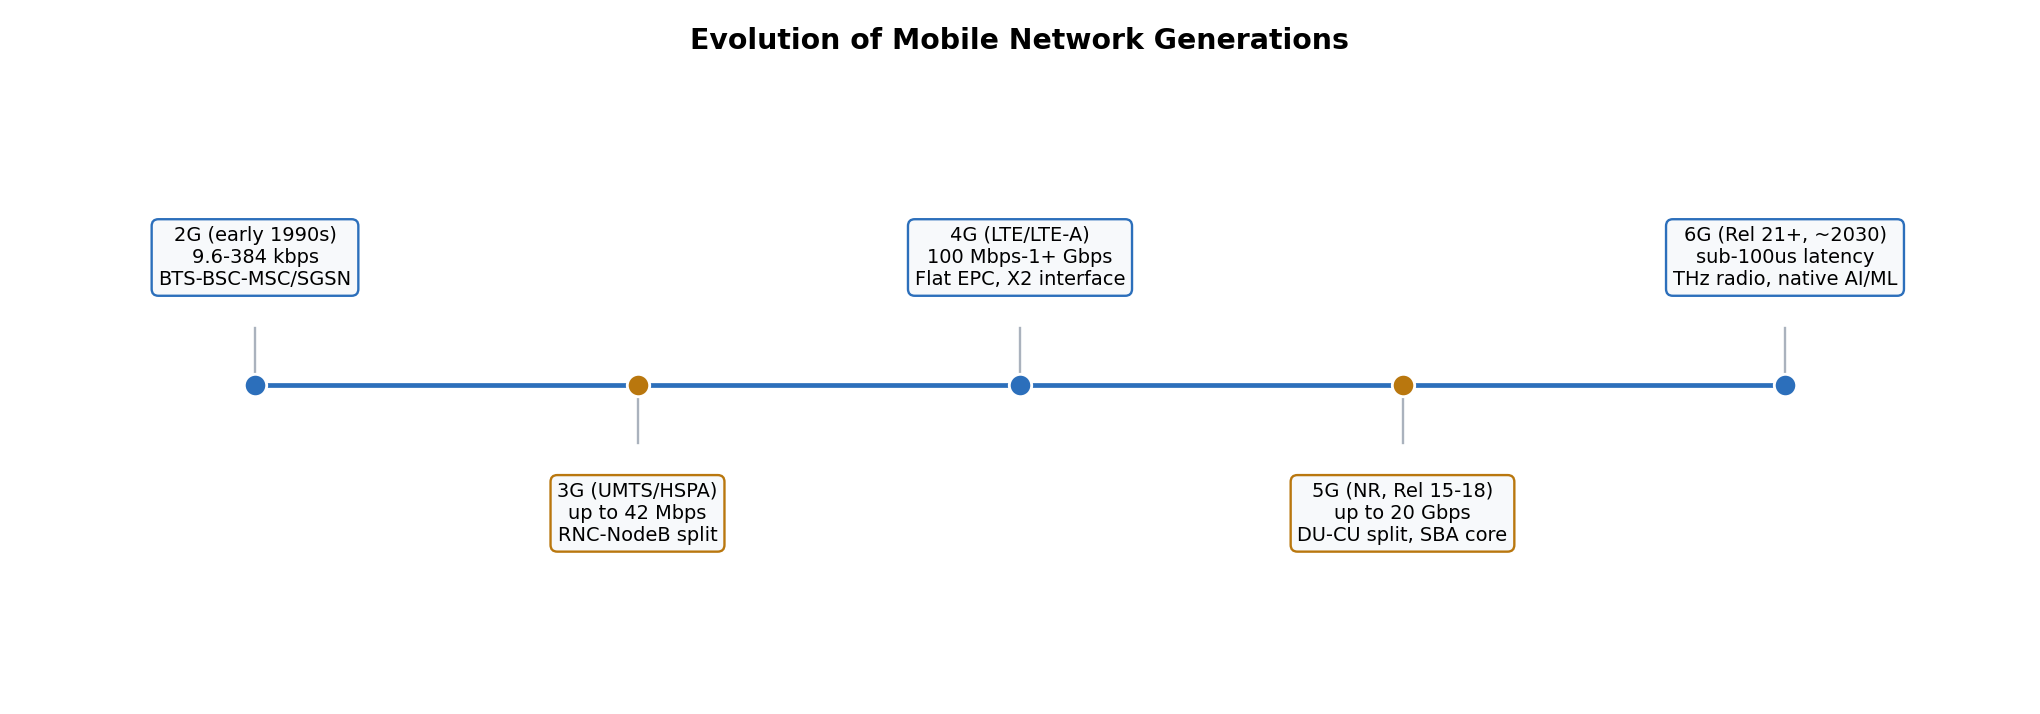
\includegraphics[width=0.85\textwidth]{figures/fig_1_1.png}
    \caption{Evolution of Mobile Network Generations --- Evolution of mobile network generations from 2G to the envisioned 6G, showing peak data rate and defining architectural change at each step.}
    \label{fig:1_1}
\end{figure}

\begin{figure}[htbp]
    \centering
    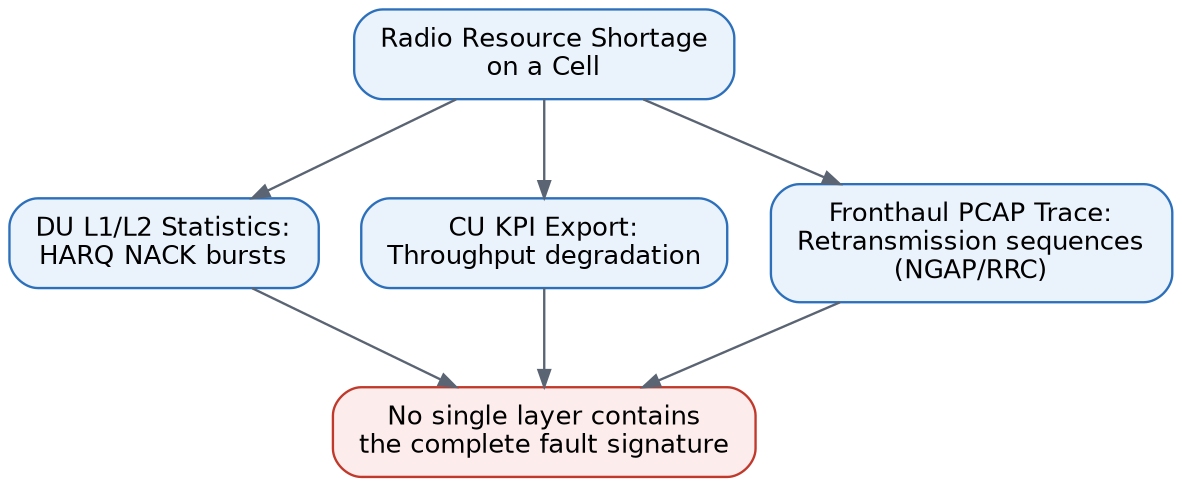
\includegraphics[width=0.85\textwidth]{figures/fig_1_2.png}
    \caption{Multi-Layer Fault Signature Propagation --- A single radio-resource fault propagates distinct, incomplete signatures into each of the three telemetry domains, motivating multi-modal detection.}
    \label{fig:1_2}
\end{figure}

\begin{figure}[htbp]
    \centering
    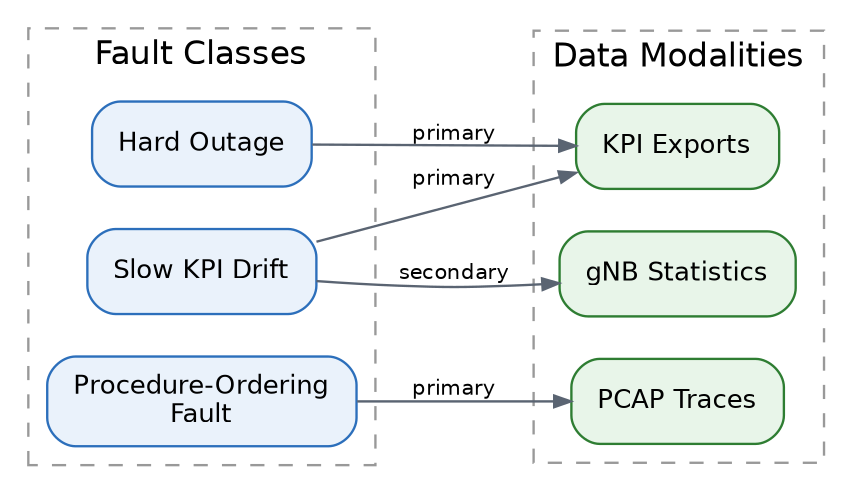
\includegraphics[width=0.85\textwidth]{figures/fig_1_3.png}
    \caption{Complementary Fault Coverage of the Three Modalities --- Mapping of the three targeted fault classes to their primary detecting modality, illustrating why no single data source covers the full fault taxonomy.}
    \label{fig:1_3}
\end{figure}

% ---------------- Chapter 2 ----------------
\begin{figure}[htbp]
    \centering
    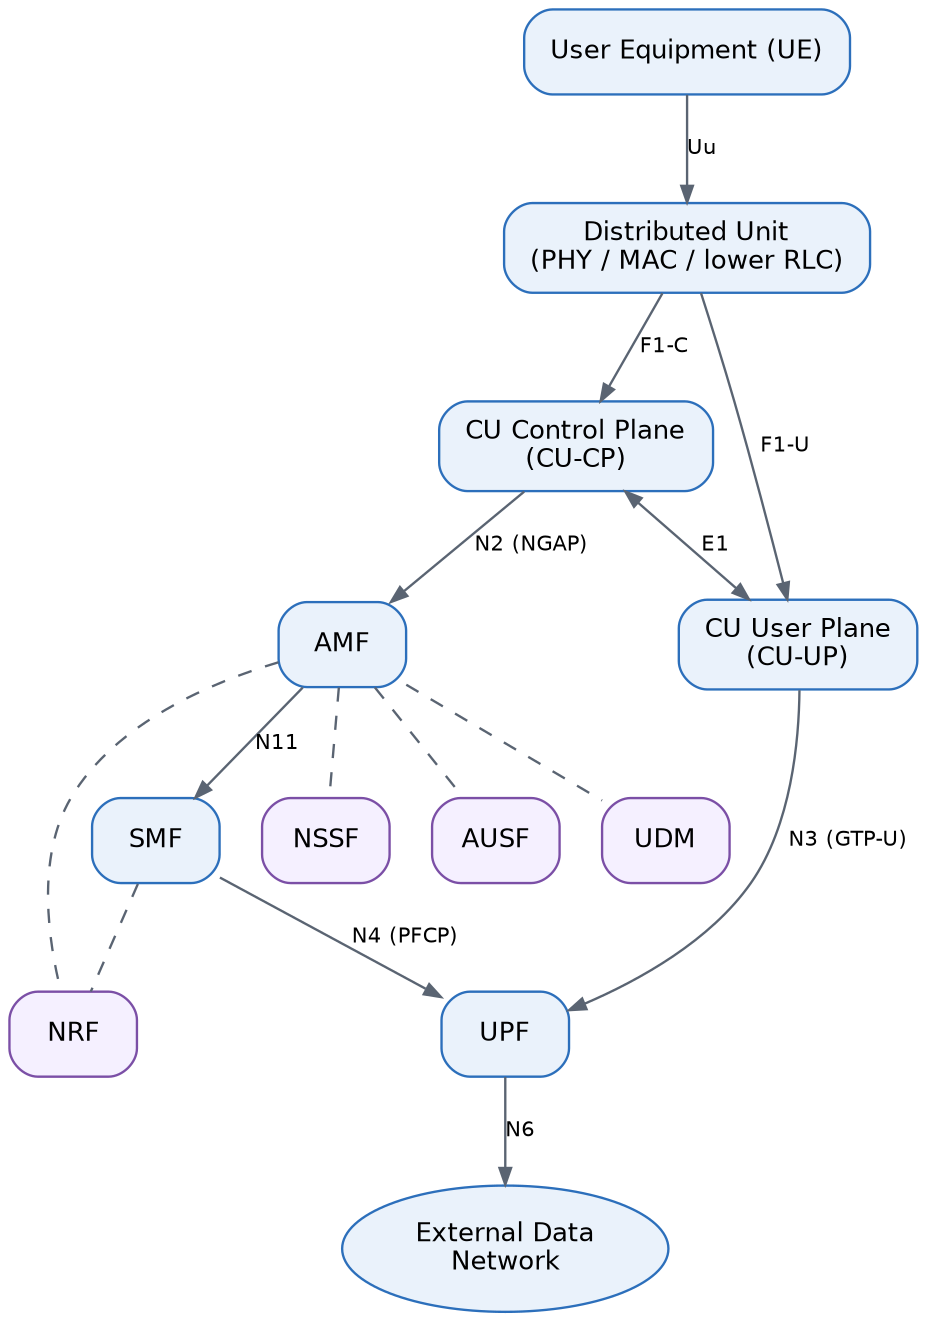
\includegraphics[width=0.85\textwidth]{figures/fig_2_1.png}
    \caption{5G Network Architecture (NG-RAN + 5GC) --- 5G system architecture showing the disaggregated NG-RAN (DU/CU-CP/CU-UP) and the Service-Based Architecture of the 5G Core.}
    \label{fig:2_1}
\end{figure}

\begin{figure}[htbp]
    \centering
    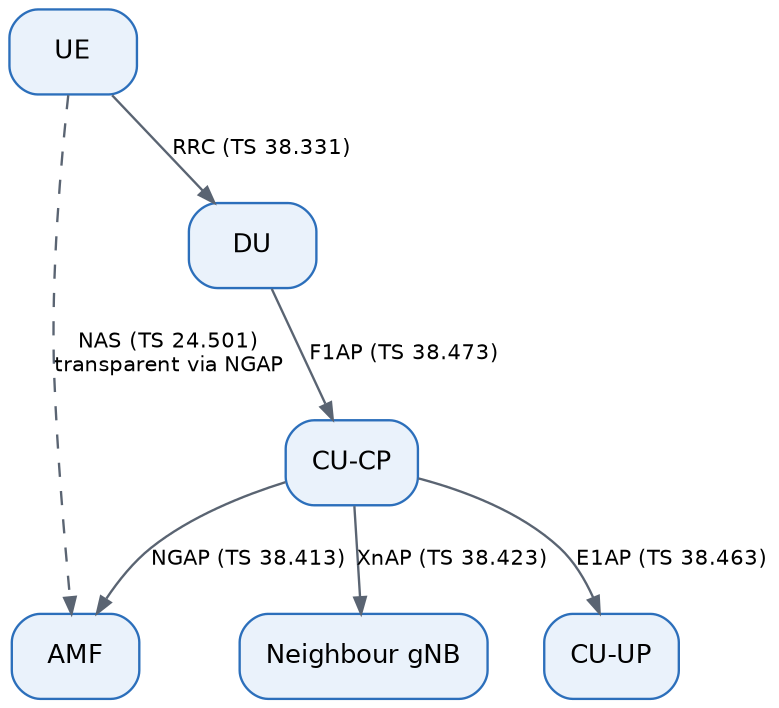
\includegraphics[width=0.85\textwidth]{figures/fig_2_2.png}
    \caption{Six Protocol Interfaces Mapped to Network Nodes --- The six 5G-NR protocol interfaces parsed by the PCAP Parser, mapped to their governing 3GPP specification and network-node endpoints.}
    \label{fig:2_2}
\end{figure}

% ---------------- Chapter 3 ----------------
\begin{figure}[htbp]
    \centering
    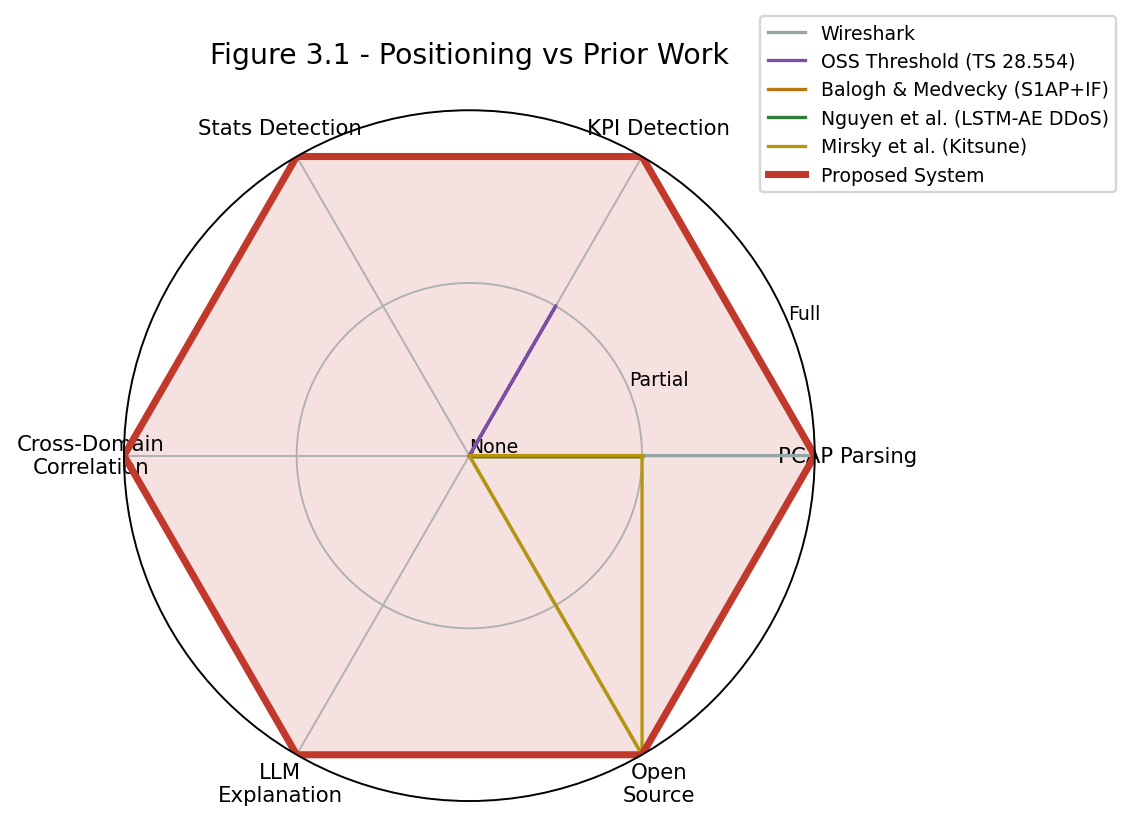
\includegraphics[width=0.85\textwidth]{figures/fig_3_1.png}
    \caption{Positioning Comparison vs. Prior Work --- Radar comparison of the proposed system against five representative prior systems across the five positioning axes of Table 3.1.}
    \label{fig:3_1}
\end{figure}

% ---------------- Chapter 4 ----------------
\begin{figure}[htbp]
    \centering
    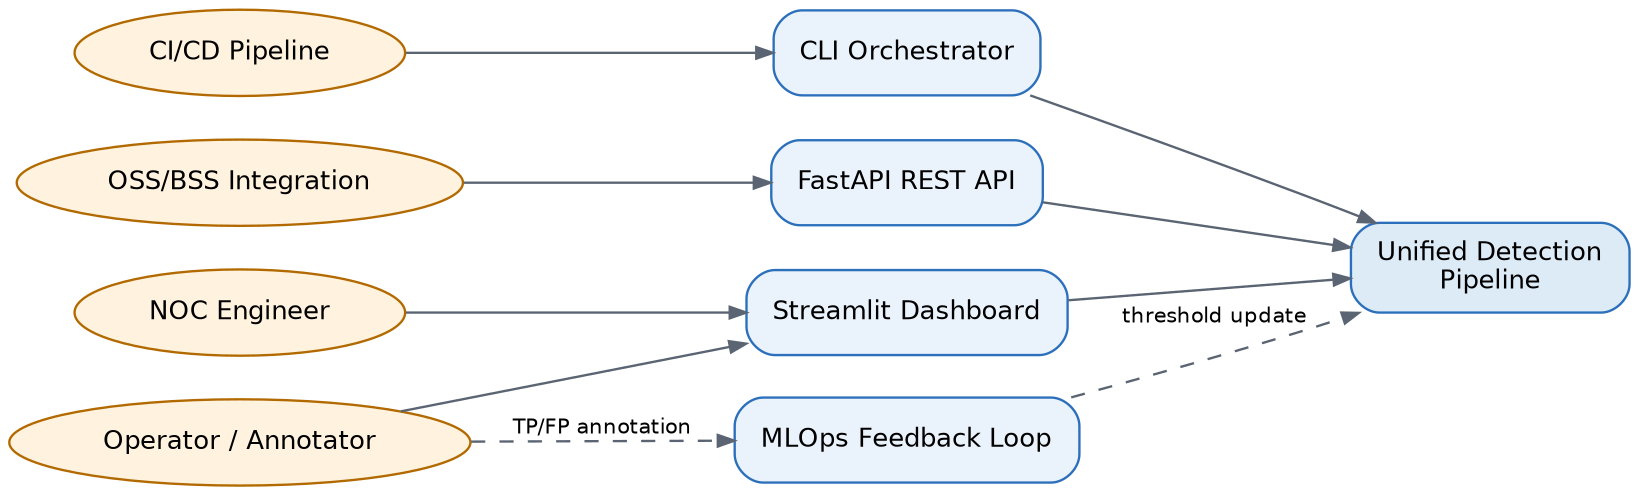
\includegraphics[width=0.85\textwidth]{figures/fig_4_1.png}
    \caption{Use Case Diagram --- Actors and access interfaces for the Unified Telecom Analyzer, tracing each functional requirement to its consuming role.}
    \label{fig:4_1}
\end{figure}

% ---------------- Chapter 5 ----------------
\begin{figure}[htbp]
    \centering
    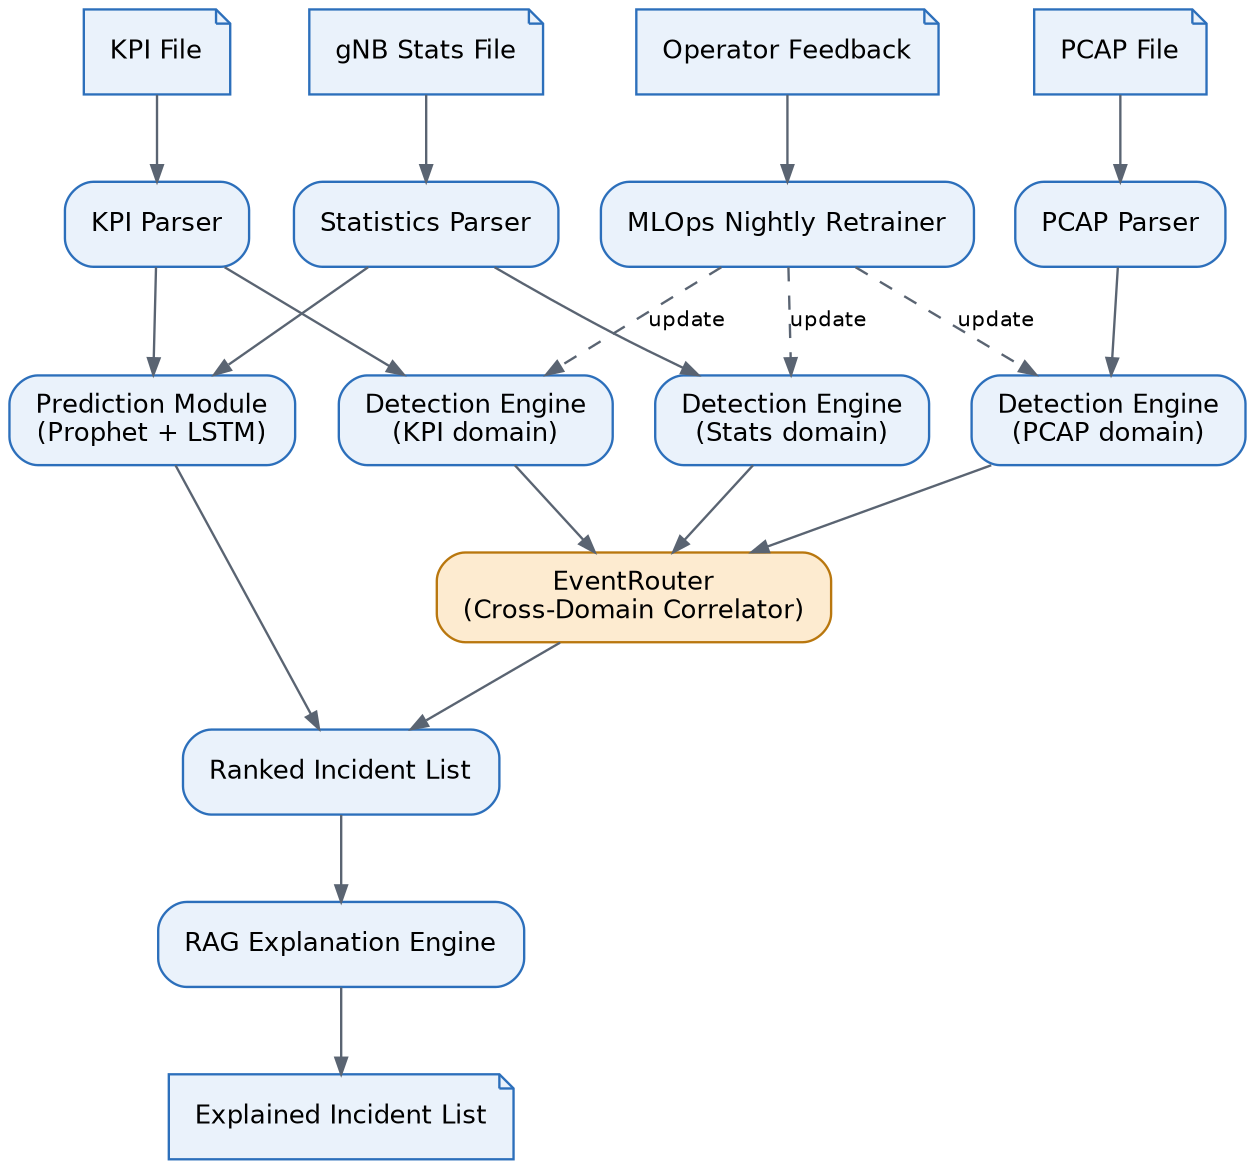
\includegraphics[width=0.85\textwidth]{figures/fig_5_1.png}
    \caption{Unified Pipeline End-to-End Control Flow --- End-to-end control flow of the Unified Telecom Analyzer, showing the Parse to Detect to Correlate to Explain pipeline with parallel Prediction and MLOps feedback branches.}
    \label{fig:5_1}
\end{figure}

\begin{figure}[htbp]
    \centering
    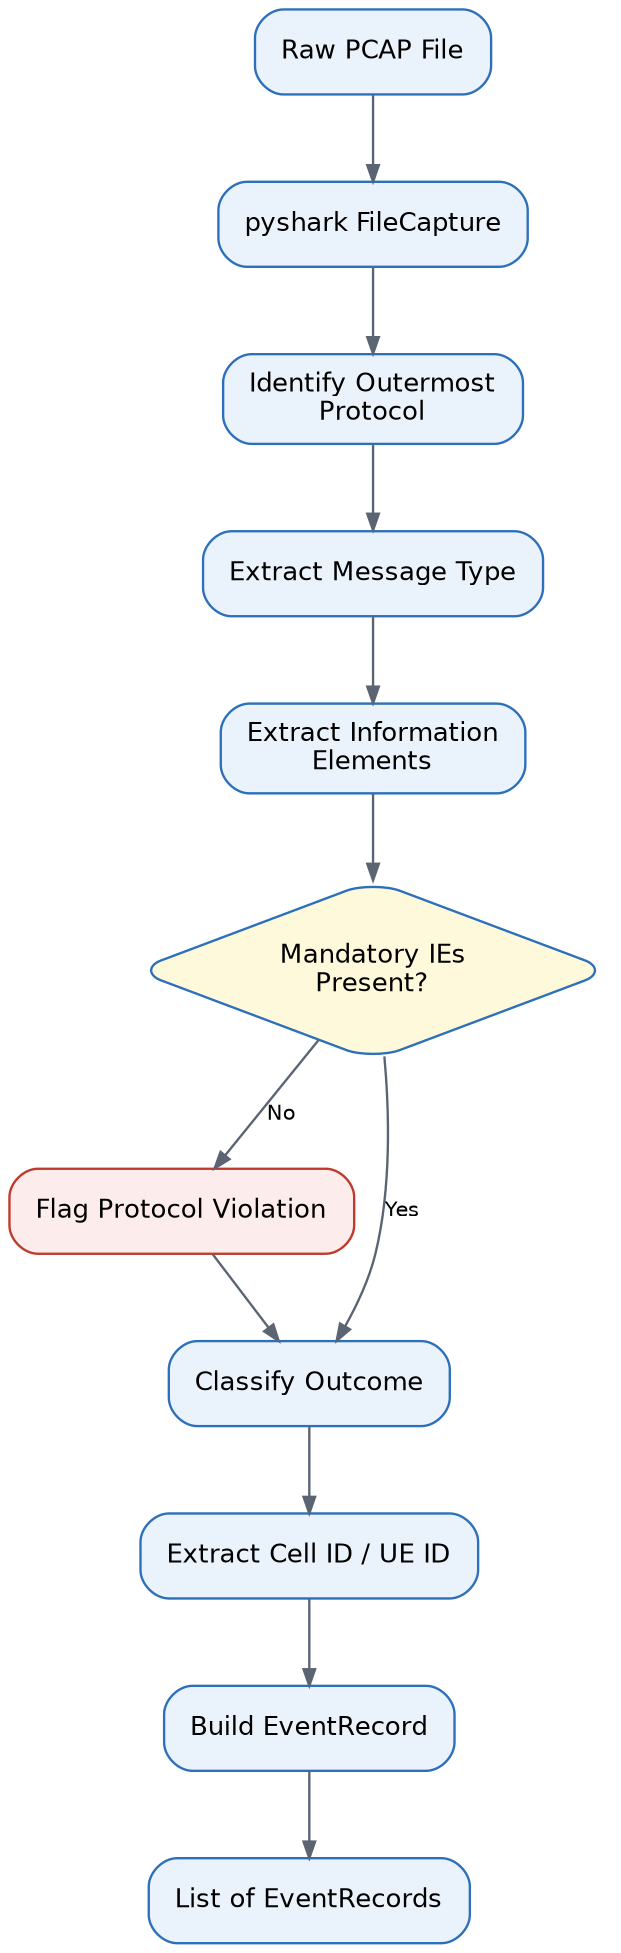
\includegraphics[width=0.85\textwidth]{figures/fig_5_2.png}
    \caption{PCAP Parser Workflow --- PCAP Parser processing workflow, including the spec-alignment branch that flags protocol violations independently of the anomaly ensemble.}
    \label{fig:5_2}
\end{figure}

\begin{figure}[htbp]
    \centering
    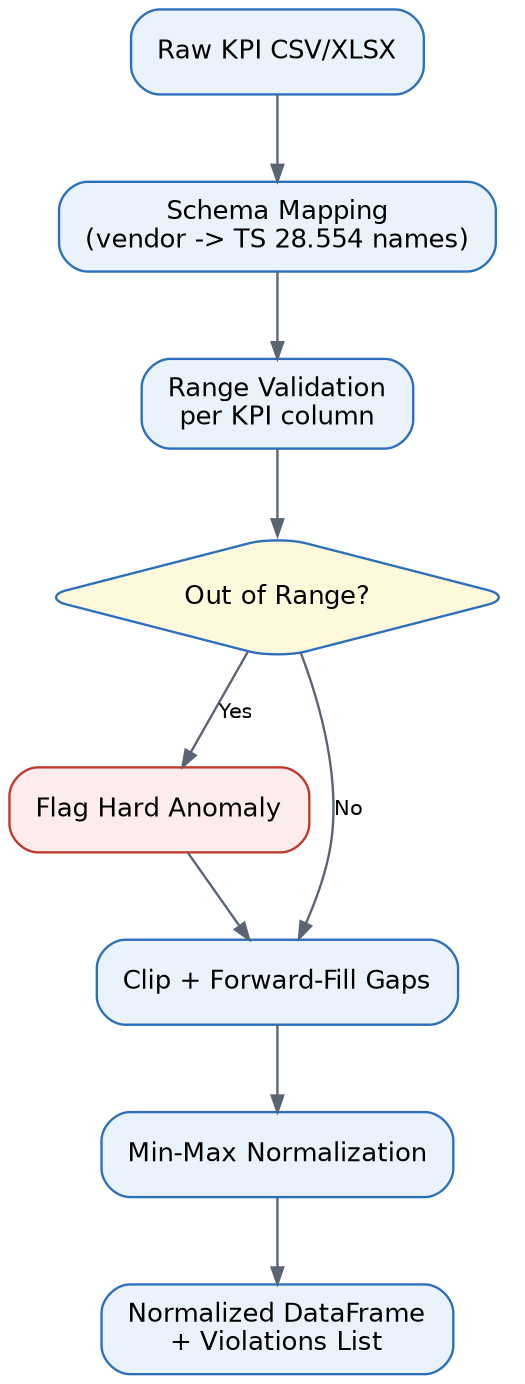
\includegraphics[width=0.85\textwidth]{figures/fig_5_3.png}
    \caption{KPI Parser Three-Stage Pipeline --- KPI Parser three-stage processing pipeline: schema mapping, range validation, and normalization.}
    \label{fig:5_3}
\end{figure}

\begin{figure}[htbp]
    \centering
    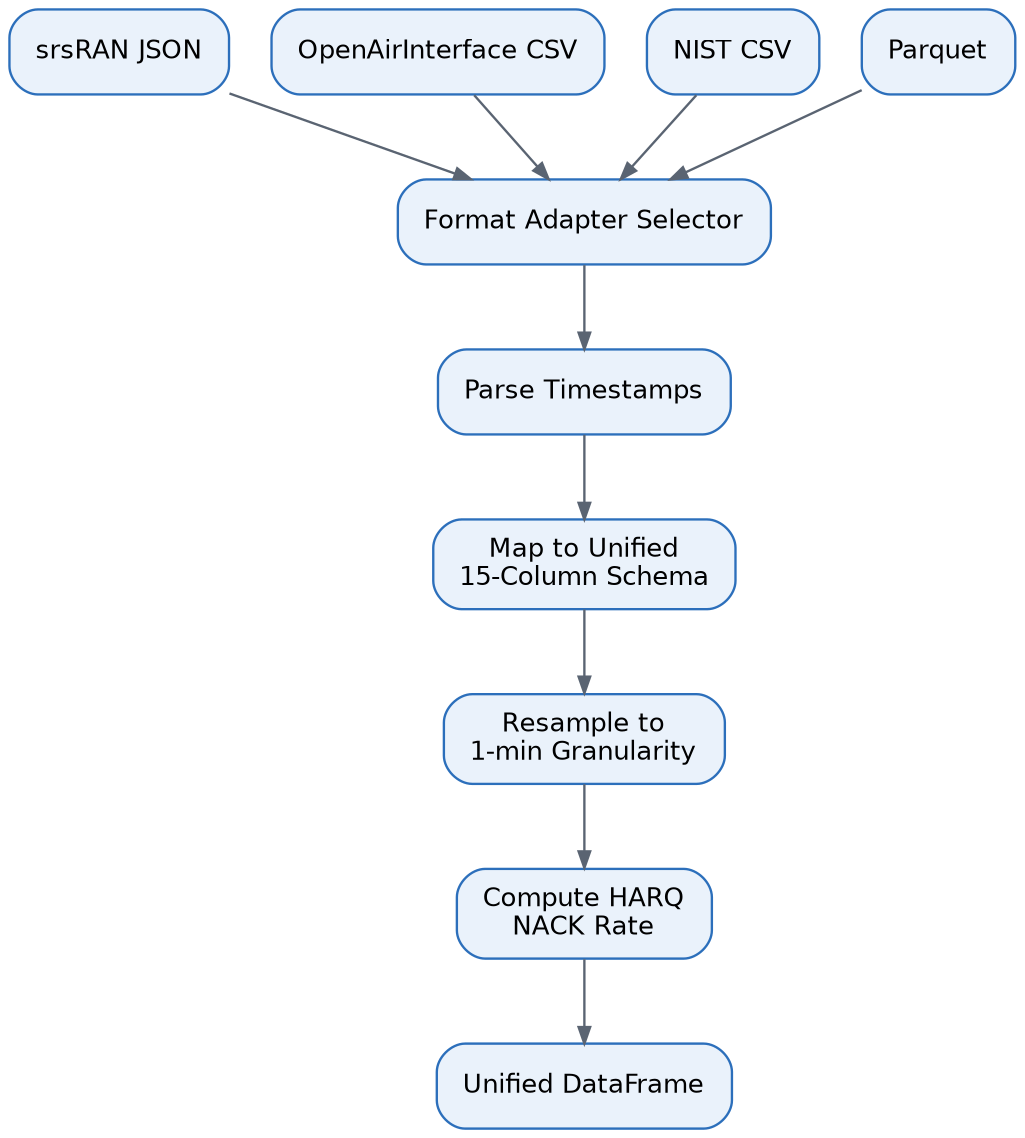
\includegraphics[width=0.85\textwidth]{figures/fig_5_4.png}
    \caption{Statistics Parser Multi-Format Adapter Architecture --- Statistics Parser adapter architecture unifying four input formats into a single 15-column schema.}
    \label{fig:5_4}
\end{figure}

\begin{figure}[htbp]
    \centering
    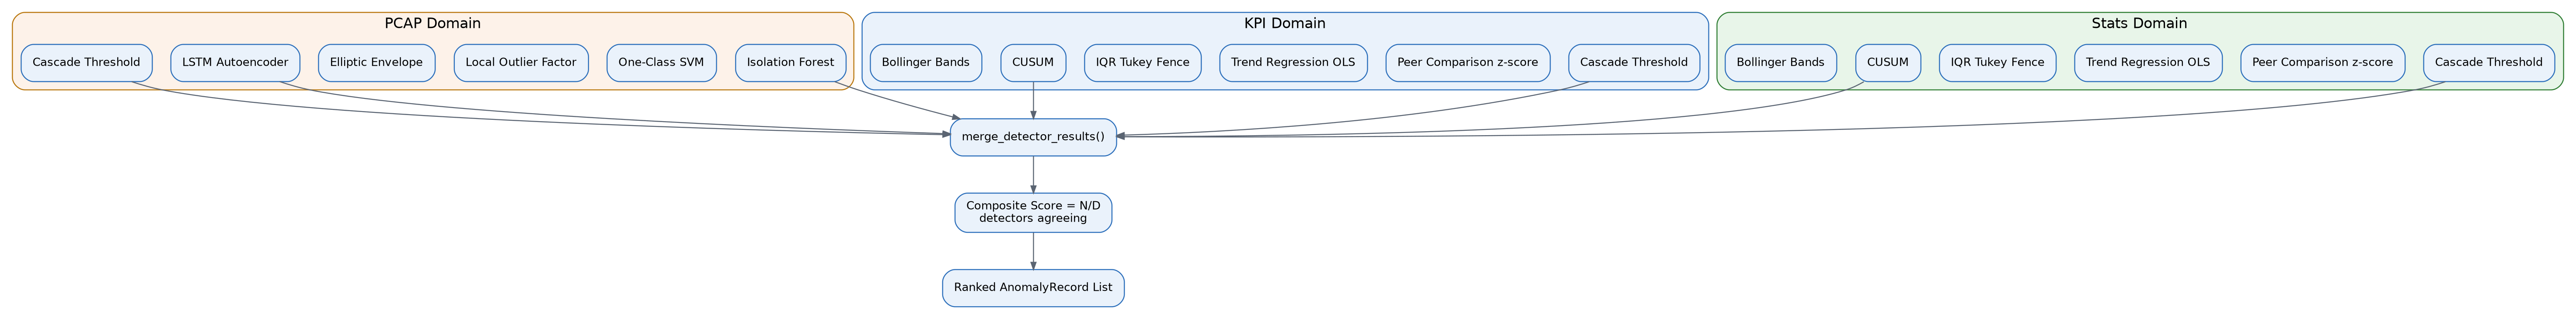
\includegraphics[width=0.85\textwidth]{figures/fig_5_5.png}
    \caption{18-Detector Ensemble Architecture --- 18-detector ensemble architecture: six algorithm families instantiated across three data domains, merged into a composite severity score.}
    \label{fig:5_5}
\end{figure}

\begin{figure}[htbp]
    \centering
    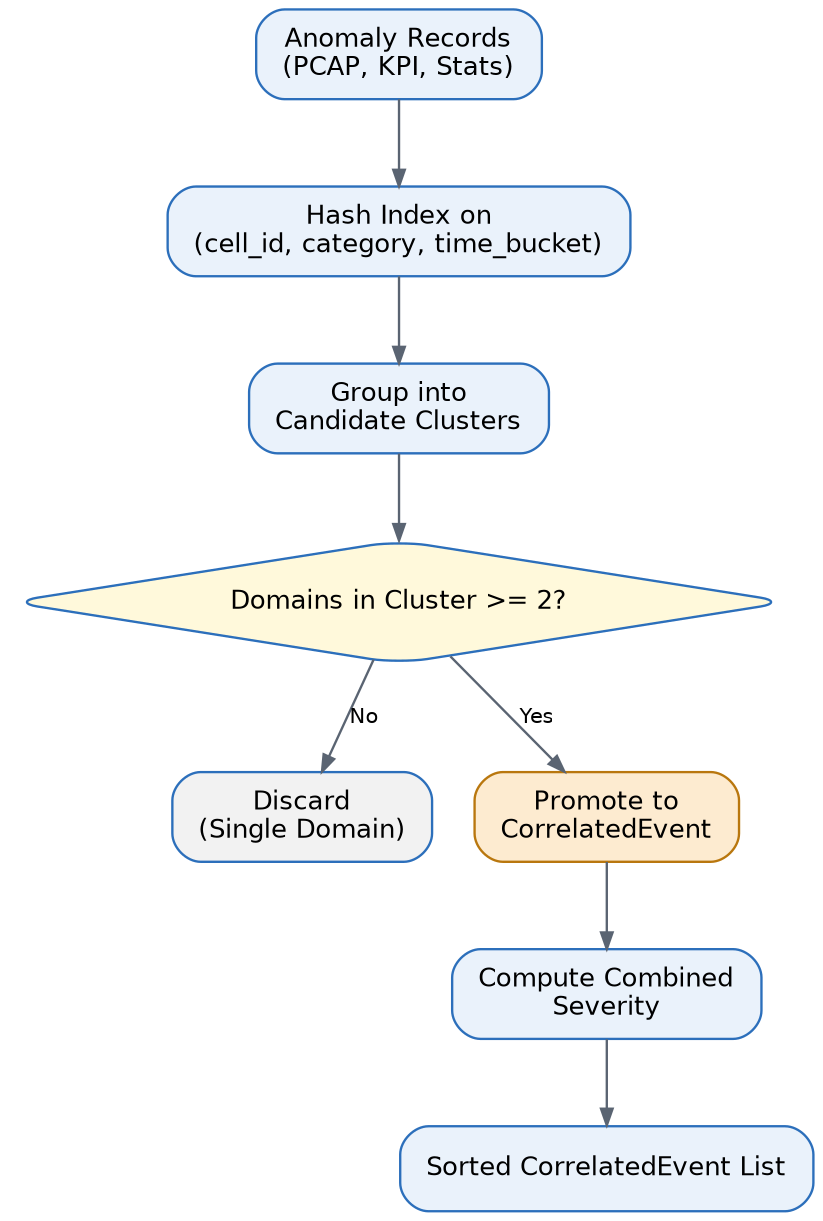
\includegraphics[width=0.85\textwidth]{figures/fig_5_6.png}
    \caption{EventRouter Cross-Domain Correlation --- EventRouter cross-domain correlation mechanism, promoting multi-domain anomaly clusters to CorrelatedEvents.}
    \label{fig:5_6}
\end{figure}

\begin{figure}[htbp]
    \centering
    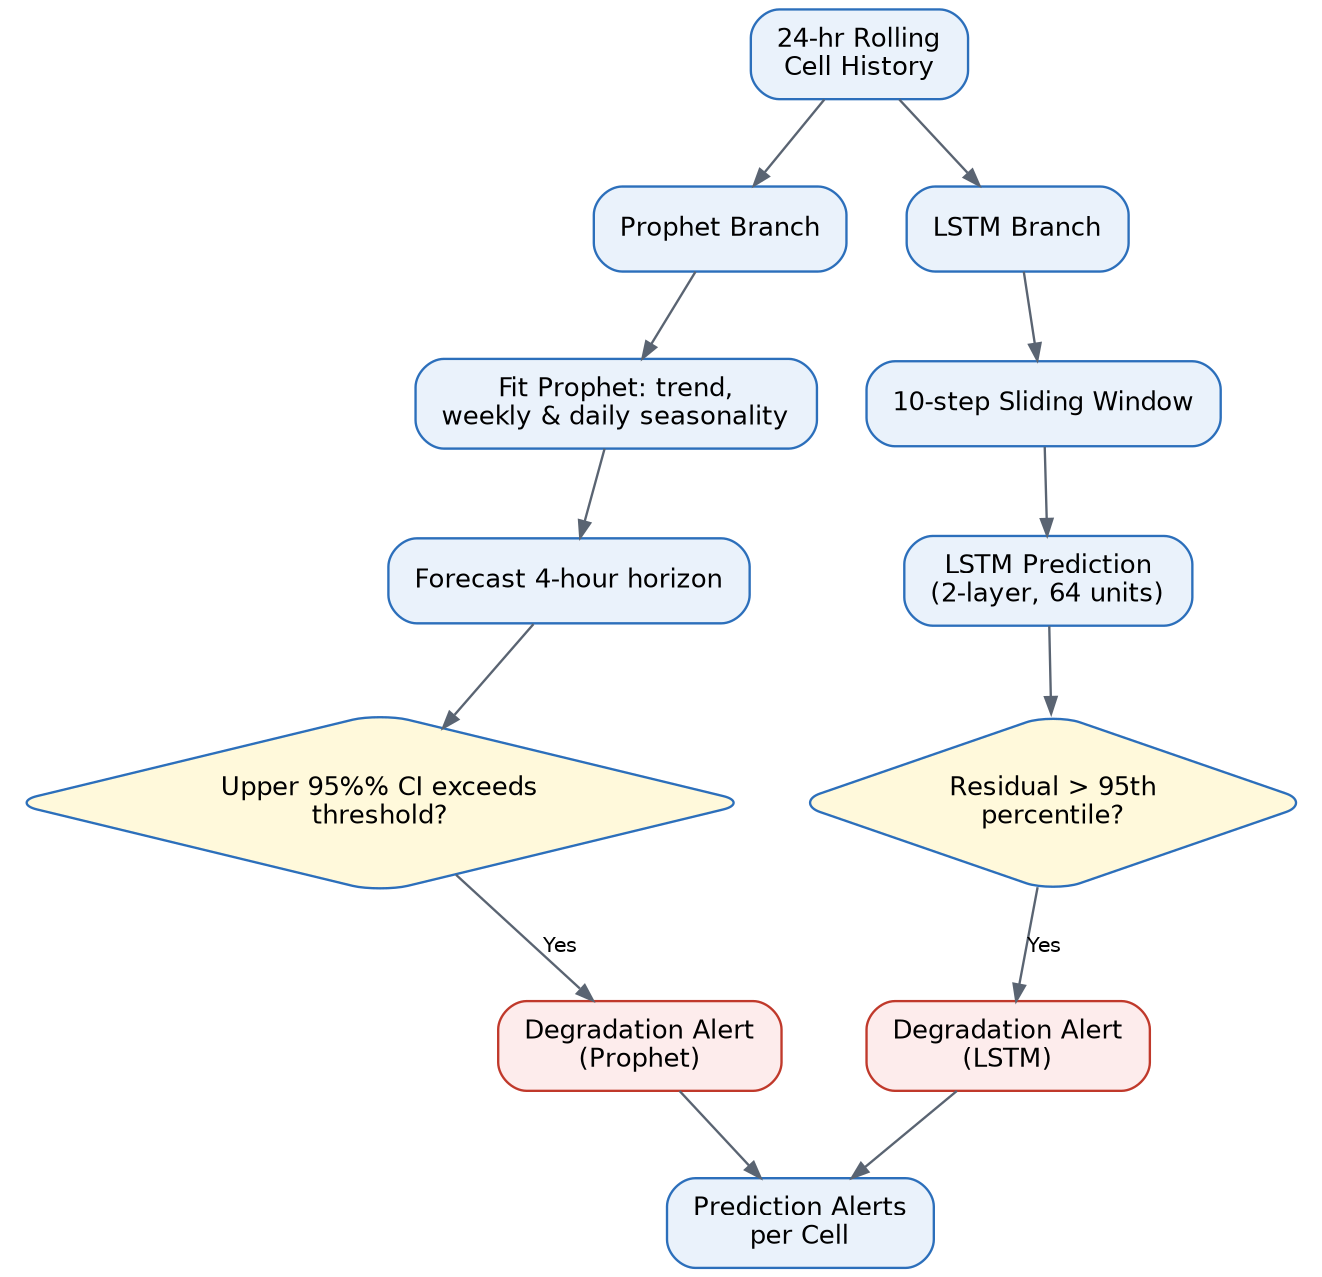
\includegraphics[width=0.85\textwidth]{figures/fig_5_7.png}
    \caption{Prediction Module Dual-Branch Design --- Dual-branch Prediction Module combining Prophet (seasonal patterns) and LSTM (non-linear sudden onset).}
    \label{fig:5_7}
\end{figure}

\begin{figure}[htbp]
    \centering
    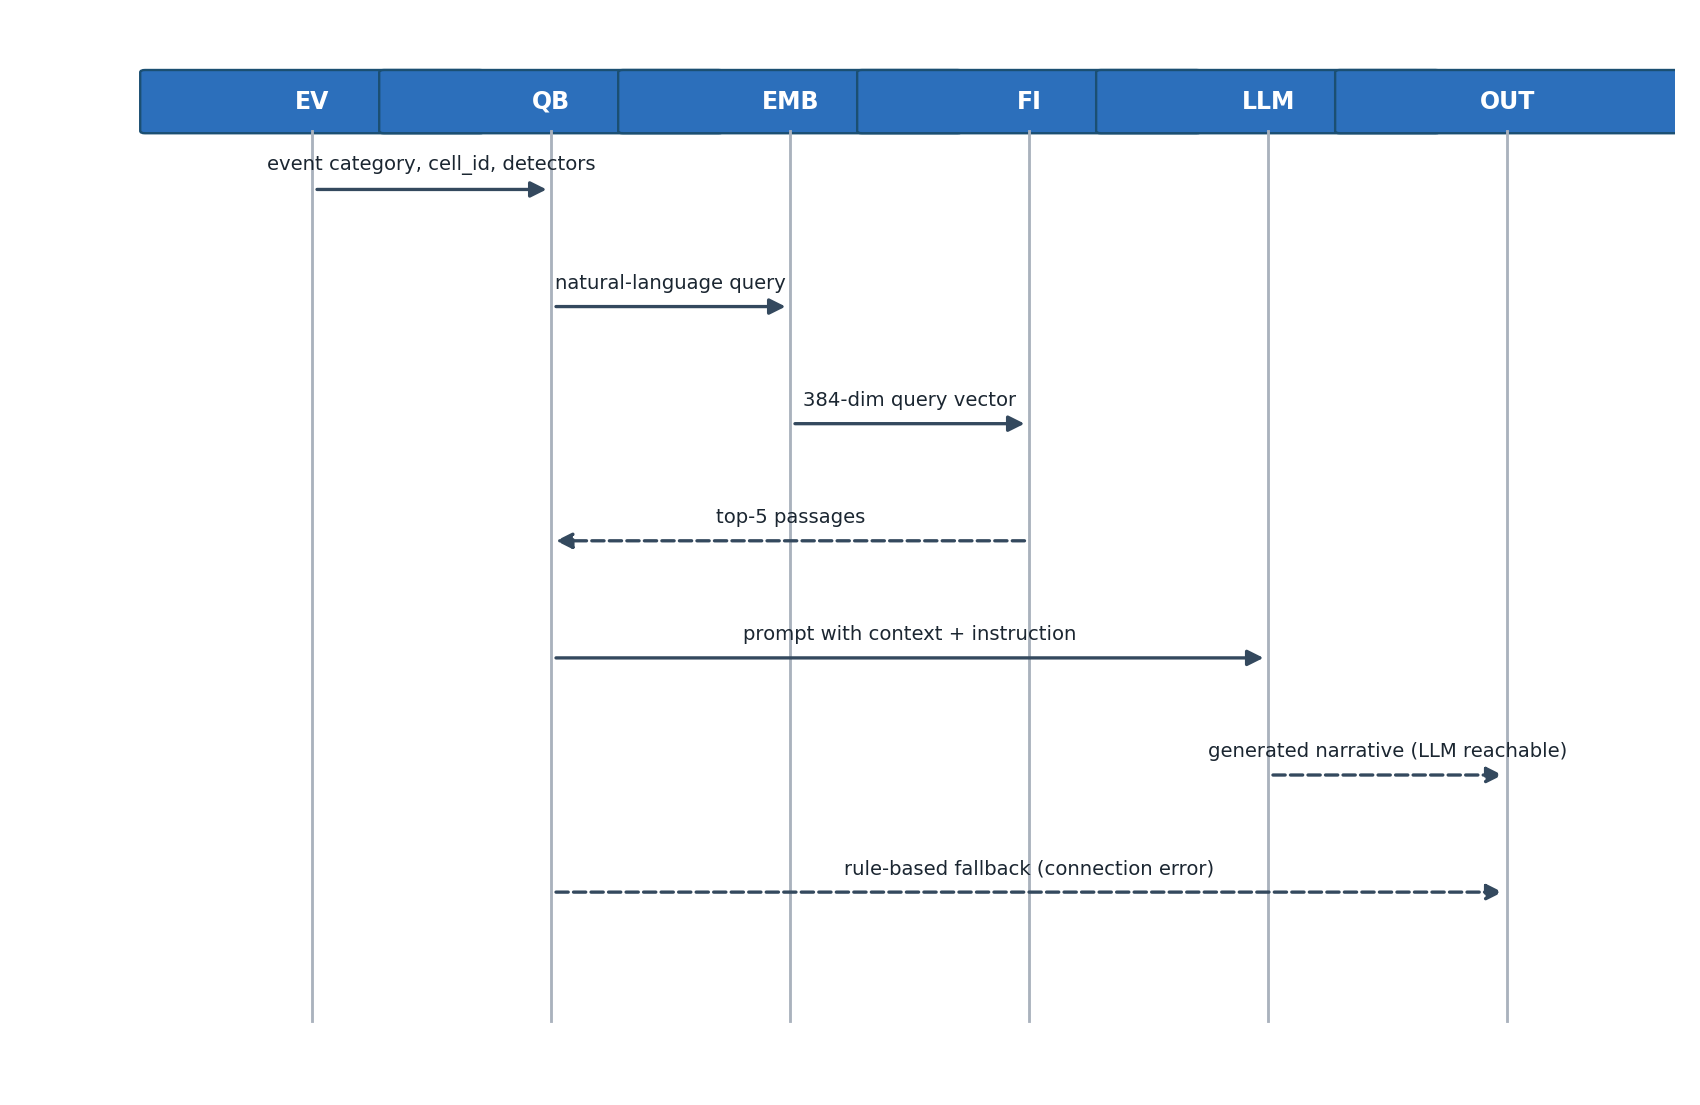
\includegraphics[width=0.85\textwidth]{figures/fig_5_8.png}
    \caption{RAG Explanation Engine Flow --- RAG Explanation Engine pipeline: query construction, FAISS retrieval, and LLM generation with offline fallback.}
    \label{fig:5_8}
\end{figure}

\begin{figure}[htbp]
    \centering
    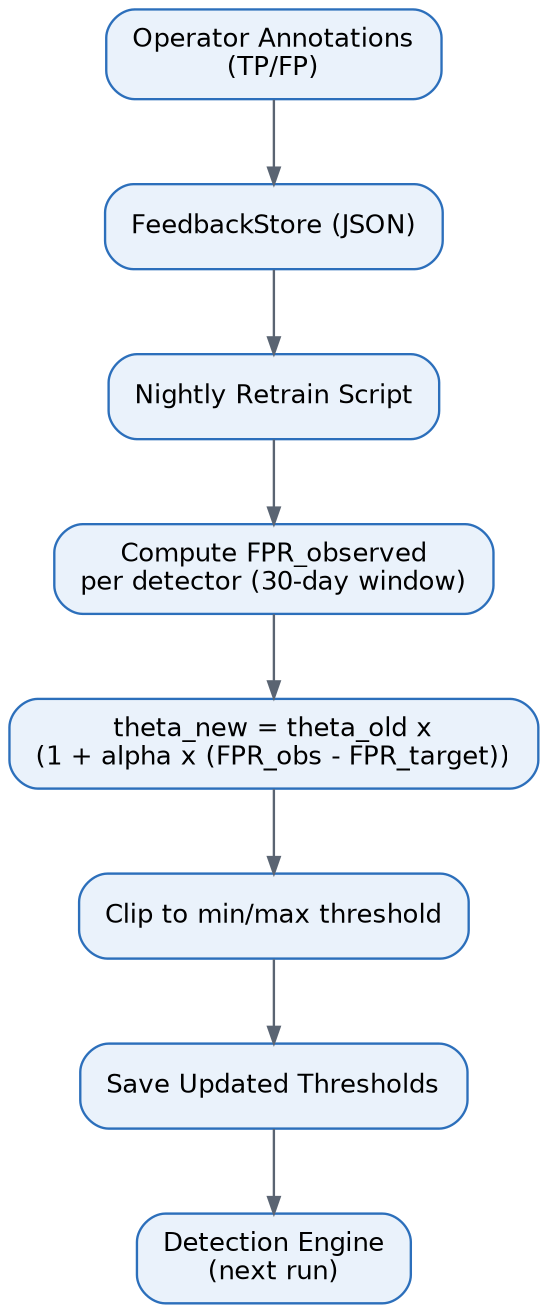
\includegraphics[width=0.85\textwidth]{figures/fig_5_9.png}
    \caption{MLOps Nightly Feedback Loop --- MLOps nightly feedback loop adjusting per-detector thresholds from operator false-positive annotations.}
    \label{fig:5_9}
\end{figure}

\begin{figure}[htbp]
    \centering
    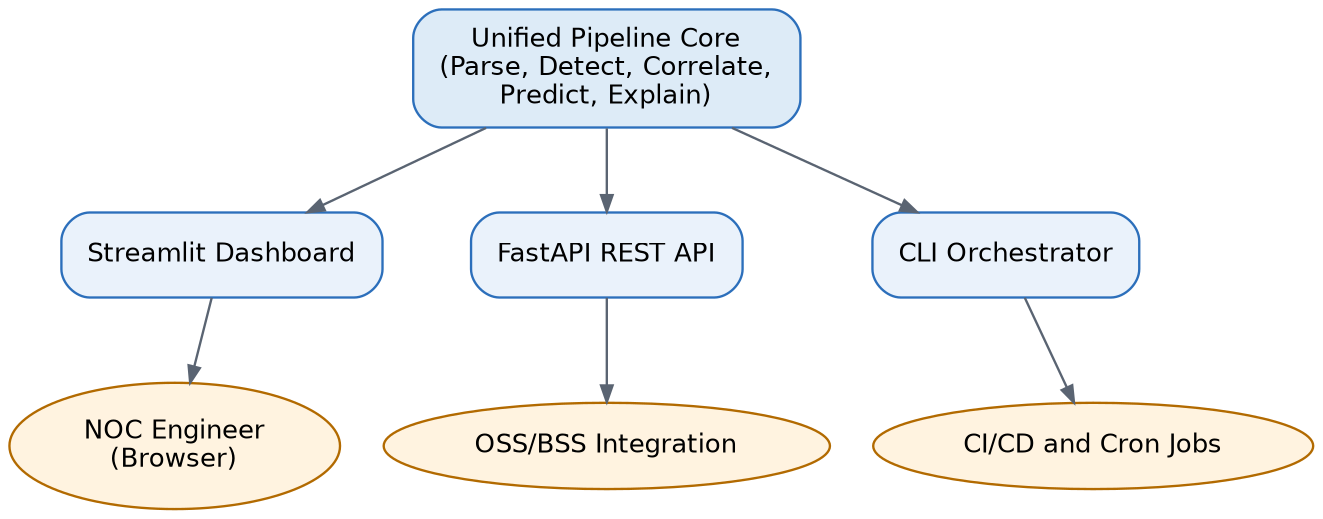
\includegraphics[width=0.85\textwidth]{figures/fig_5_10.png}
    \caption{Three Access Interfaces --- Three access interfaces (Dashboard, REST API, CLI) built on a shared pipeline core.}
    \label{fig:5_10}
\end{figure}

\begin{figure}[htbp]
    \centering
    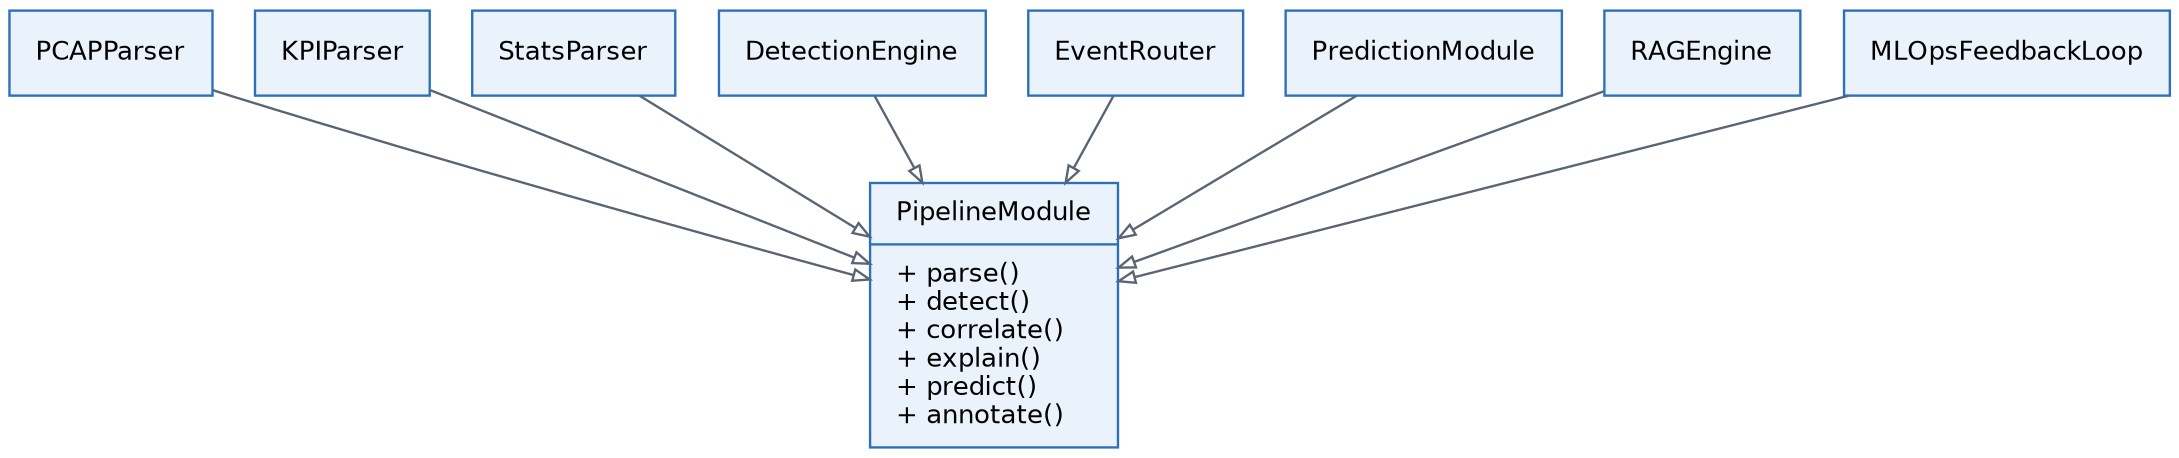
\includegraphics[width=0.85\textwidth]{figures/fig_5_11.png}
    \caption{Common Module Interface (Separation of Concerns) --- Common module interface enabling independent testing and future substitution of any pipeline component.}
    \label{fig:5_11}
\end{figure}

% ---------------- Chapter 6 ----------------
\begin{figure}[htbp]
    \centering
    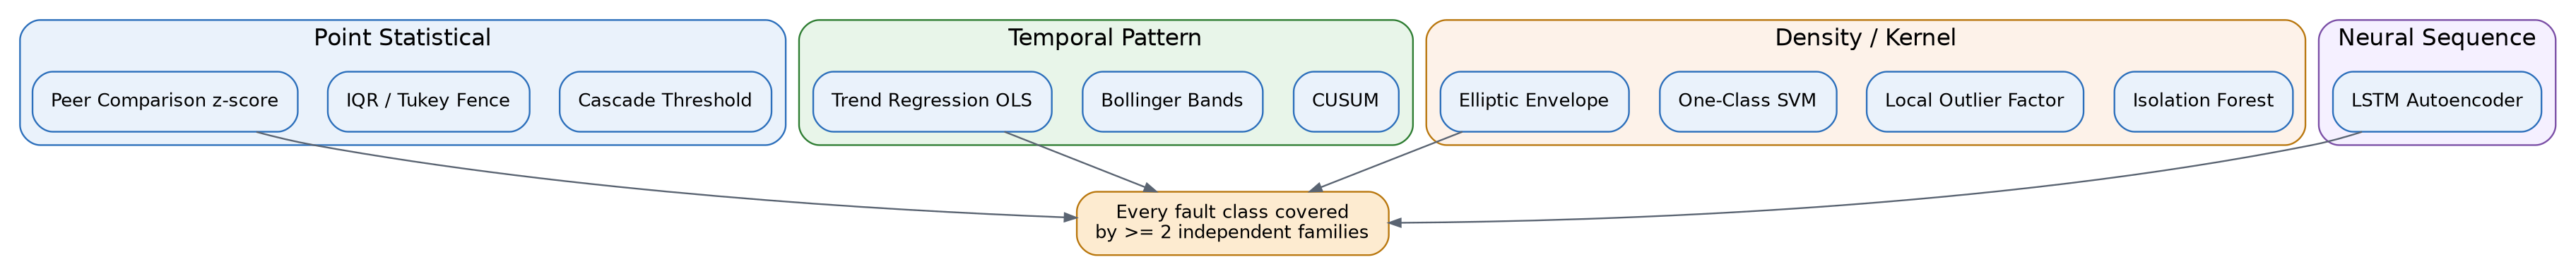
\includegraphics[width=0.85\textwidth]{figures/fig_6_1.png}
    \caption{Detector Family Taxonomy (Ensemble Coverage Principle) --- The twelve detection algorithms partitioned into four orthogonal families, the theoretical basis for the ensemble's fault-class coverage.}
    \label{fig:6_1}
\end{figure}

% ---------------- Chapter 7 ----------------
\begin{figure}[htbp]
    \centering
    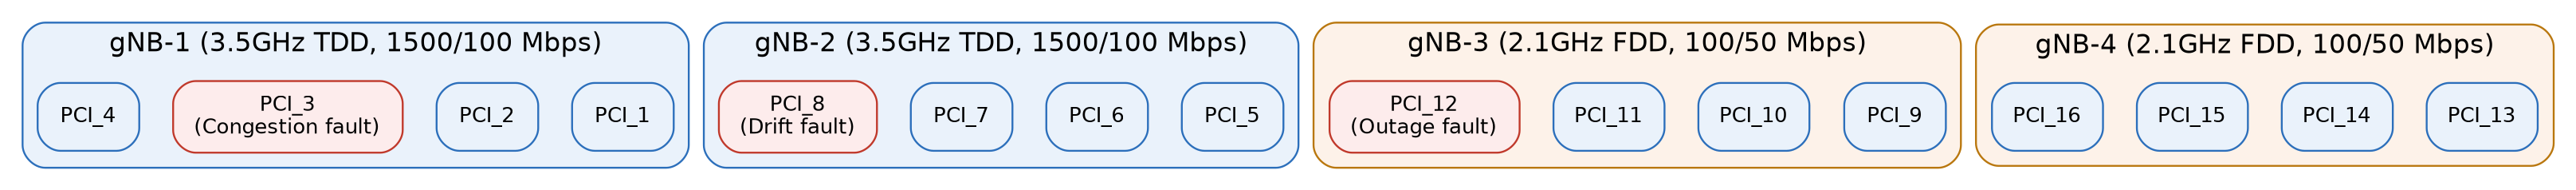
\includegraphics[width=0.85\textwidth]{figures/fig_7_1.png}
    \caption{Evaluation Network Topology --- Evaluation testbed topology: 4 gNBs / 16 cells / 64 UEs, with the three fault-injection cells highlighted.}
    \label{fig:7_1}
\end{figure}

\begin{figure}[htbp]
    \centering
    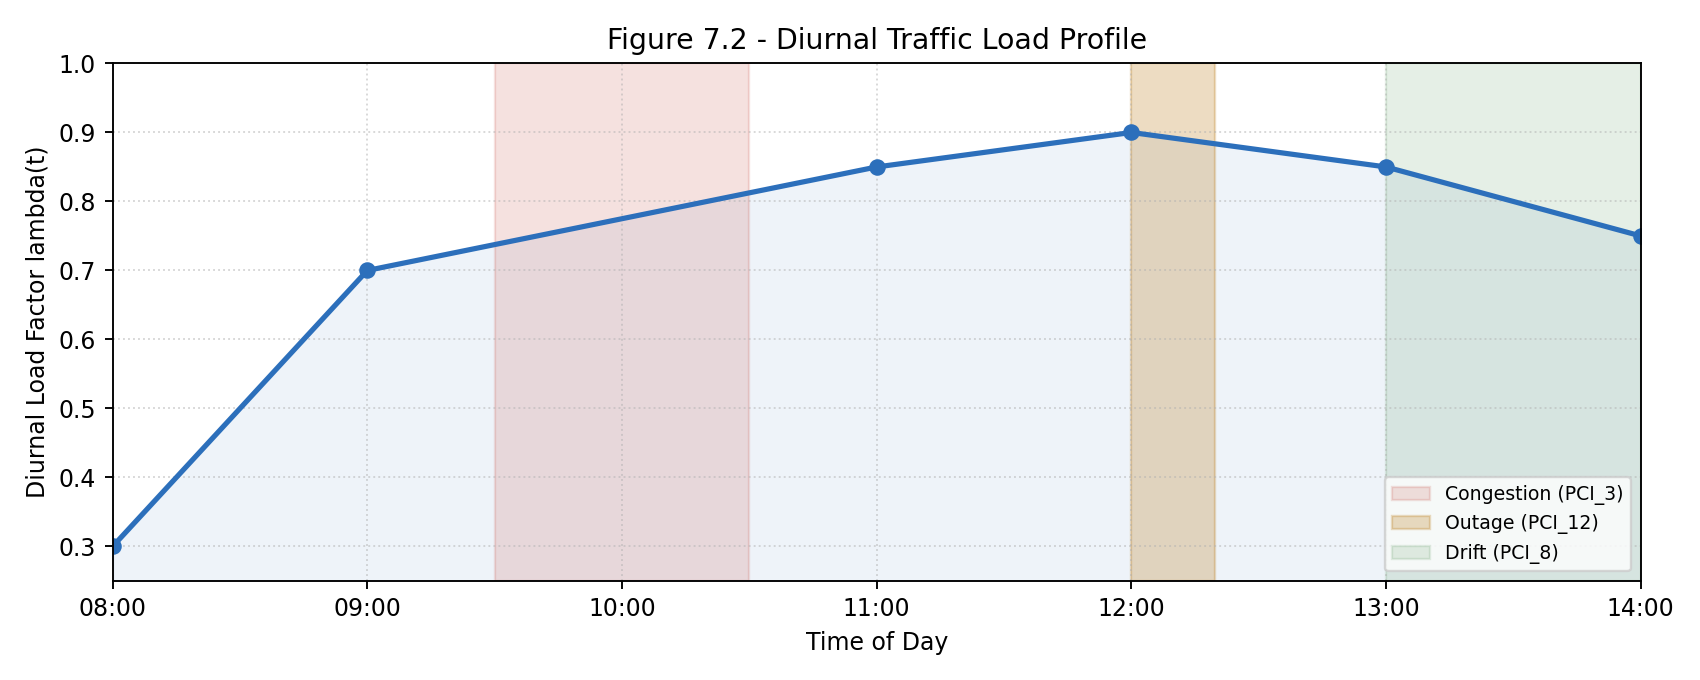
\includegraphics[width=0.85\textwidth]{figures/fig_7_2.png}
    \caption{Diurnal Traffic Load Profile --- Diurnal load factor over the 6-hour simulation window, with the three fault-injection windows marked.}
    \label{fig:7_2}
\end{figure}

\begin{figure}[htbp]
    \centering
    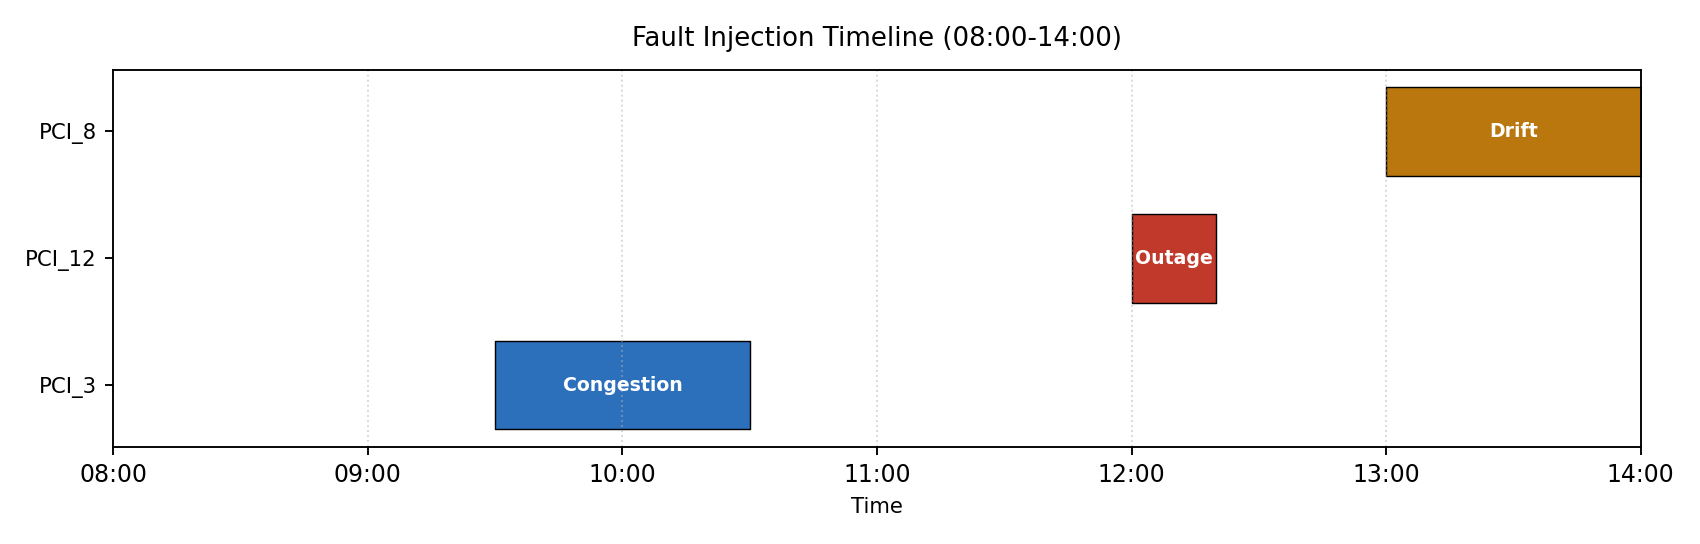
\includegraphics[width=0.85\textwidth]{figures/fig_7_3.png}
    \caption{Fault Injection Timeline --- Timeline of the three concurrent injected fault scenarios across the 6-hour evaluation window.}
    \label{fig:7_3}
\end{figure}

\begin{figure}[htbp]
    \centering
    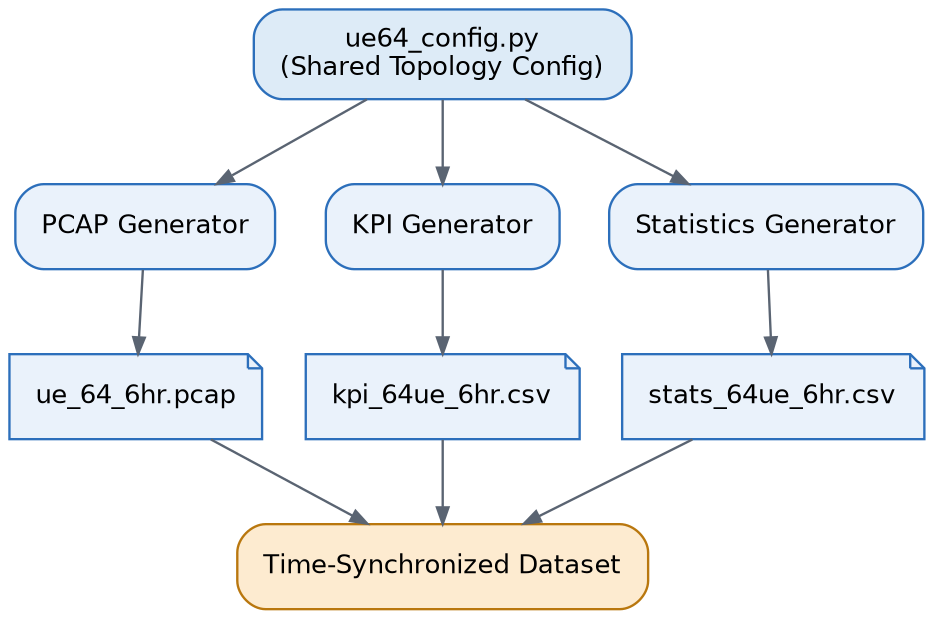
\includegraphics[width=0.85\textwidth]{figures/fig_7_4.png}
    \caption{Dataset Generation Pipeline --- Synthetic dataset generation pipeline: a single shared topology configuration produces three time-synchronized, cross-domain-consistent data files.}
    \label{fig:7_4}
\end{figure}

% ---------------- Chapter 8 ----------------
\begin{figure}[htbp]
    \centering
    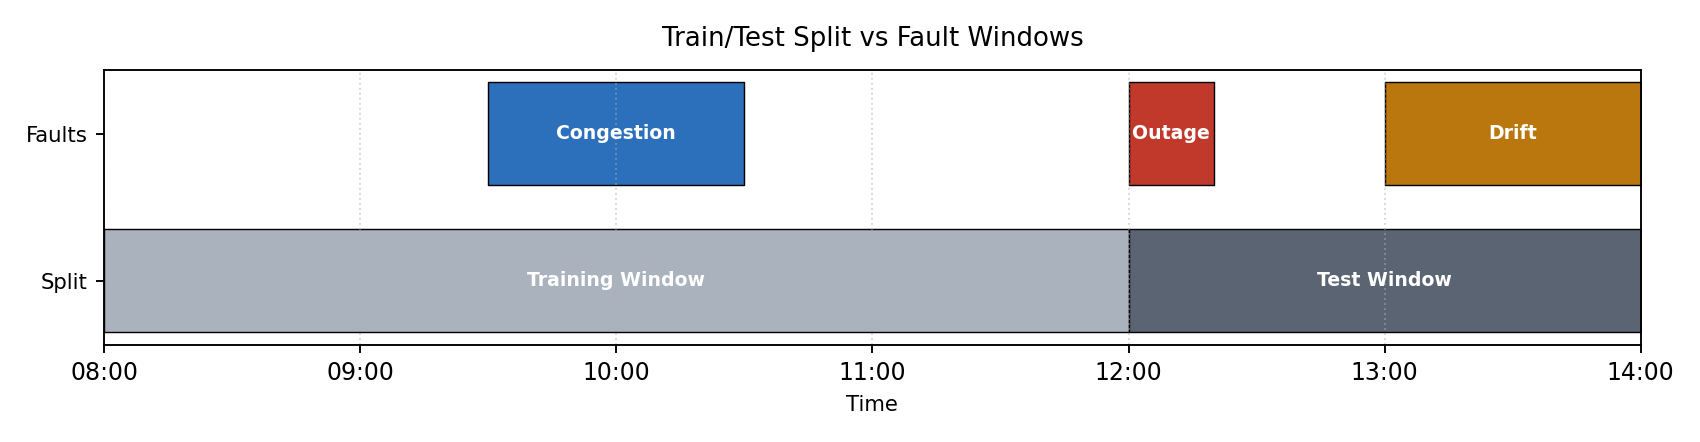
\includegraphics[width=0.85\textwidth]{figures/fig_8_1.png}
    \caption{Train/Test Temporal Split with Fault Overlay --- Temporal train/test split overlaid with the three fault windows, showing that the congestion fault straddles both windows while outage and drift fall entirely in the test window.}
    \label{fig:8_1}
\end{figure}

% ---------------- Chapter 9 ----------------
\begin{figure}[htbp]
    \centering
    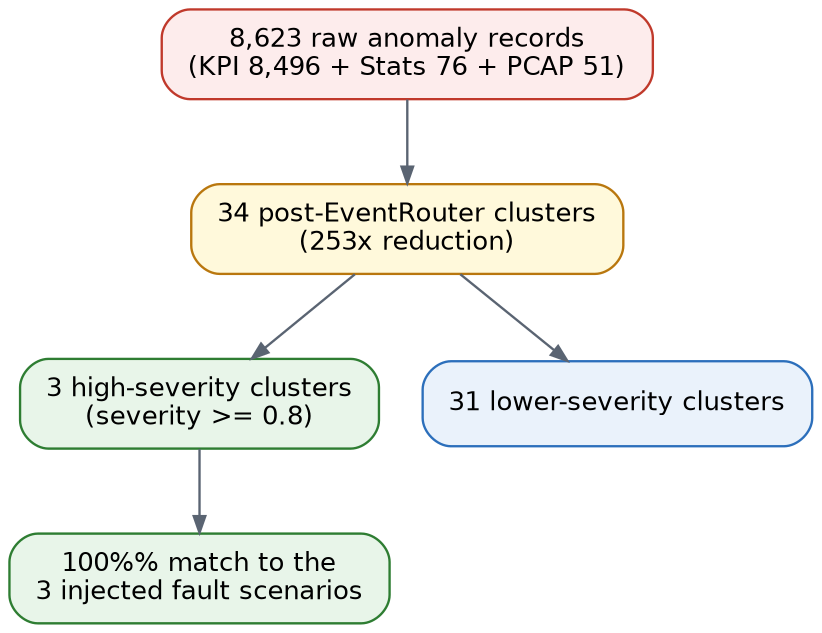
\includegraphics[width=0.85\textwidth]{figures/fig_9_1.png}
    \caption{EventRouter Alarm-Volume Reduction Funnel --- Alarm-volume reduction achieved by the EventRouter: 8,623 raw records collapse to 34 operator-visible clusters, with all three high-severity clusters correctly matching the injected faults.}
    \label{fig:9_1}
\end{figure}

\begin{figure}[htbp]
    \centering
    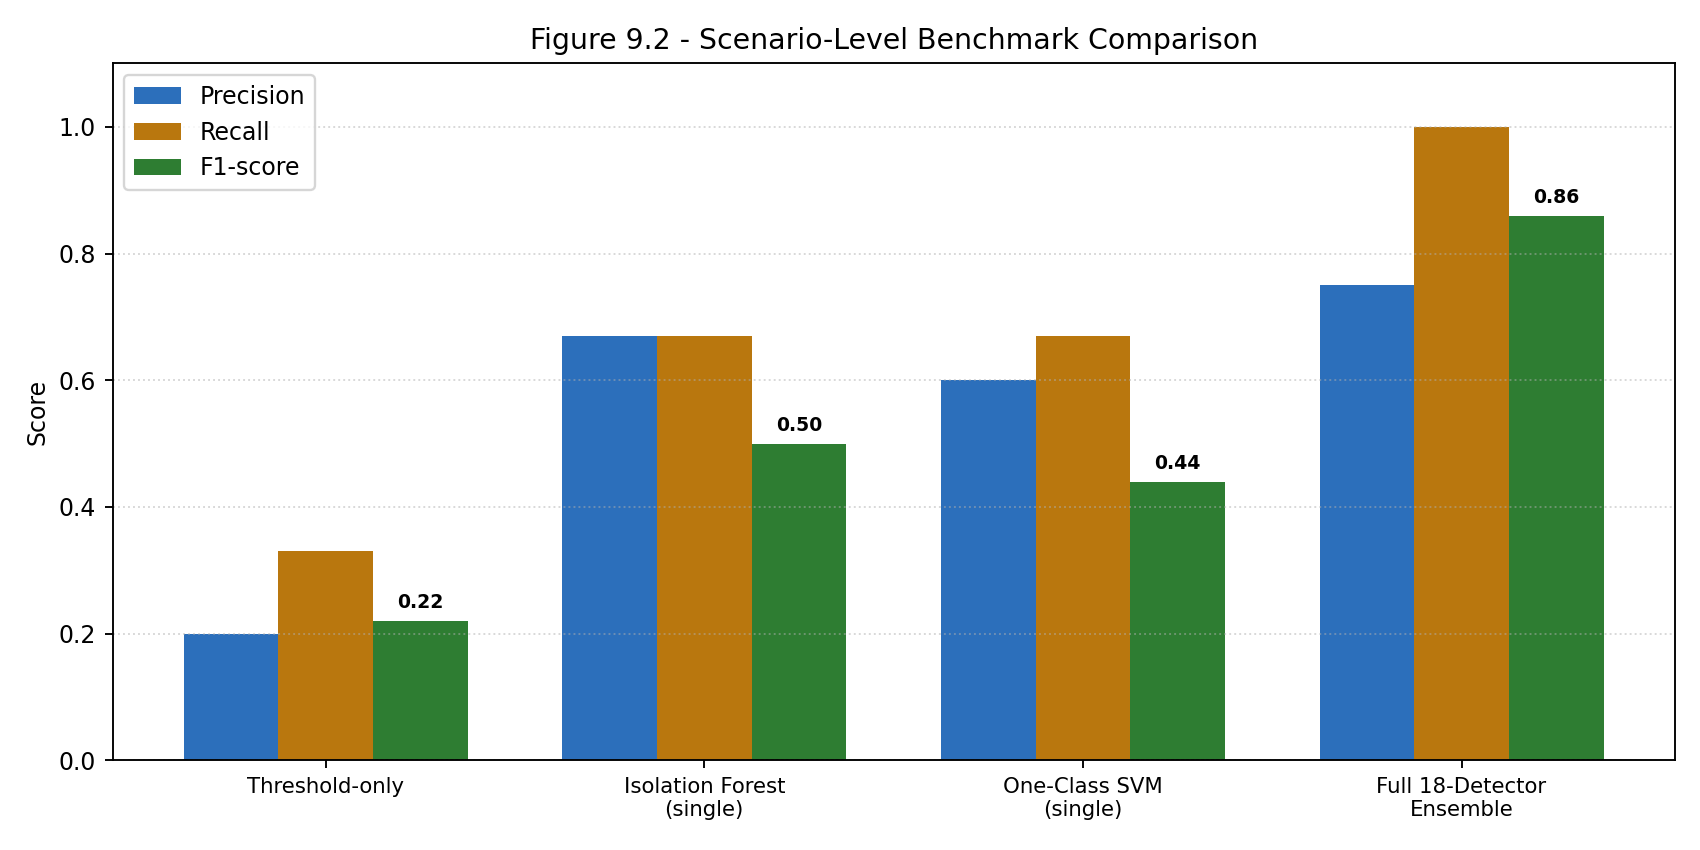
\includegraphics[width=0.85\textwidth]{figures/fig_9_2.png}
    \caption{Benchmark Comparison (Precision/Recall/F1) --- Scenario-level Precision, Recall, and F1 across the threshold-only baseline, two single-detector baselines, and the full 18-detector ensemble.}
    \label{fig:9_2}
\end{figure}

\begin{figure}[htbp]
    \centering
    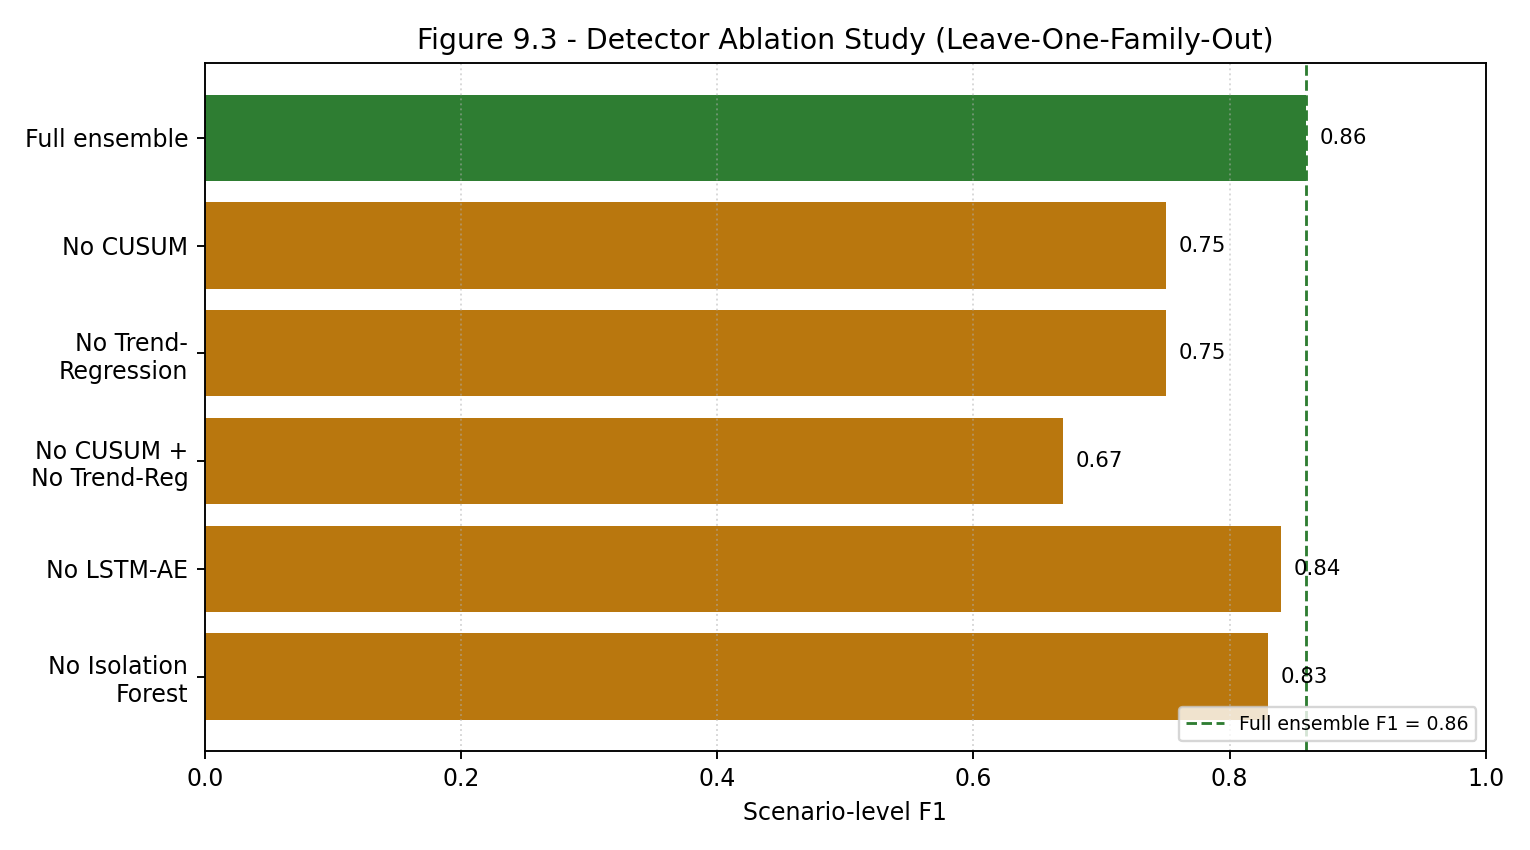
\includegraphics[width=0.85\textwidth]{figures/fig_9_3.png}
    \caption{Detector Ablation Study --- Leave-one-family-out ablation results, showing CUSUM and Trend-Regression as jointly necessary for slow-drift detection.}
    \label{fig:9_3}
\end{figure}

\begin{figure}[htbp]
    \centering
    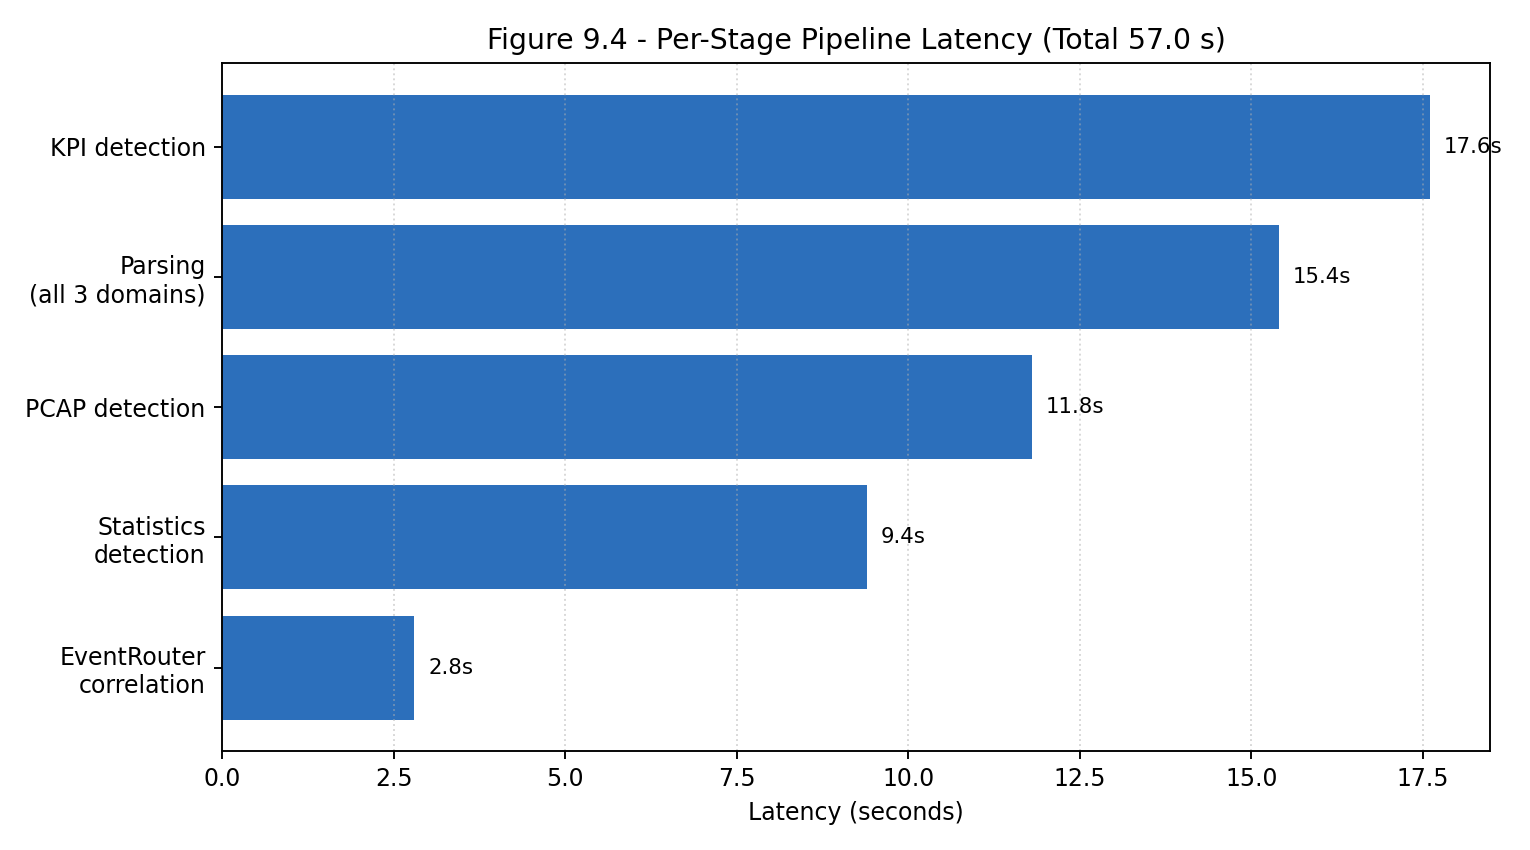
\includegraphics[width=0.85\textwidth]{figures/fig_9_4.png}
    \caption{Pipeline Latency Breakdown by Stage --- Per-stage latency breakdown of the 57-second end-to-end pipeline on the 64-UE dataset.}
    \label{fig:9_4}
\end{figure}

\begin{figure}[htbp]
    \centering
    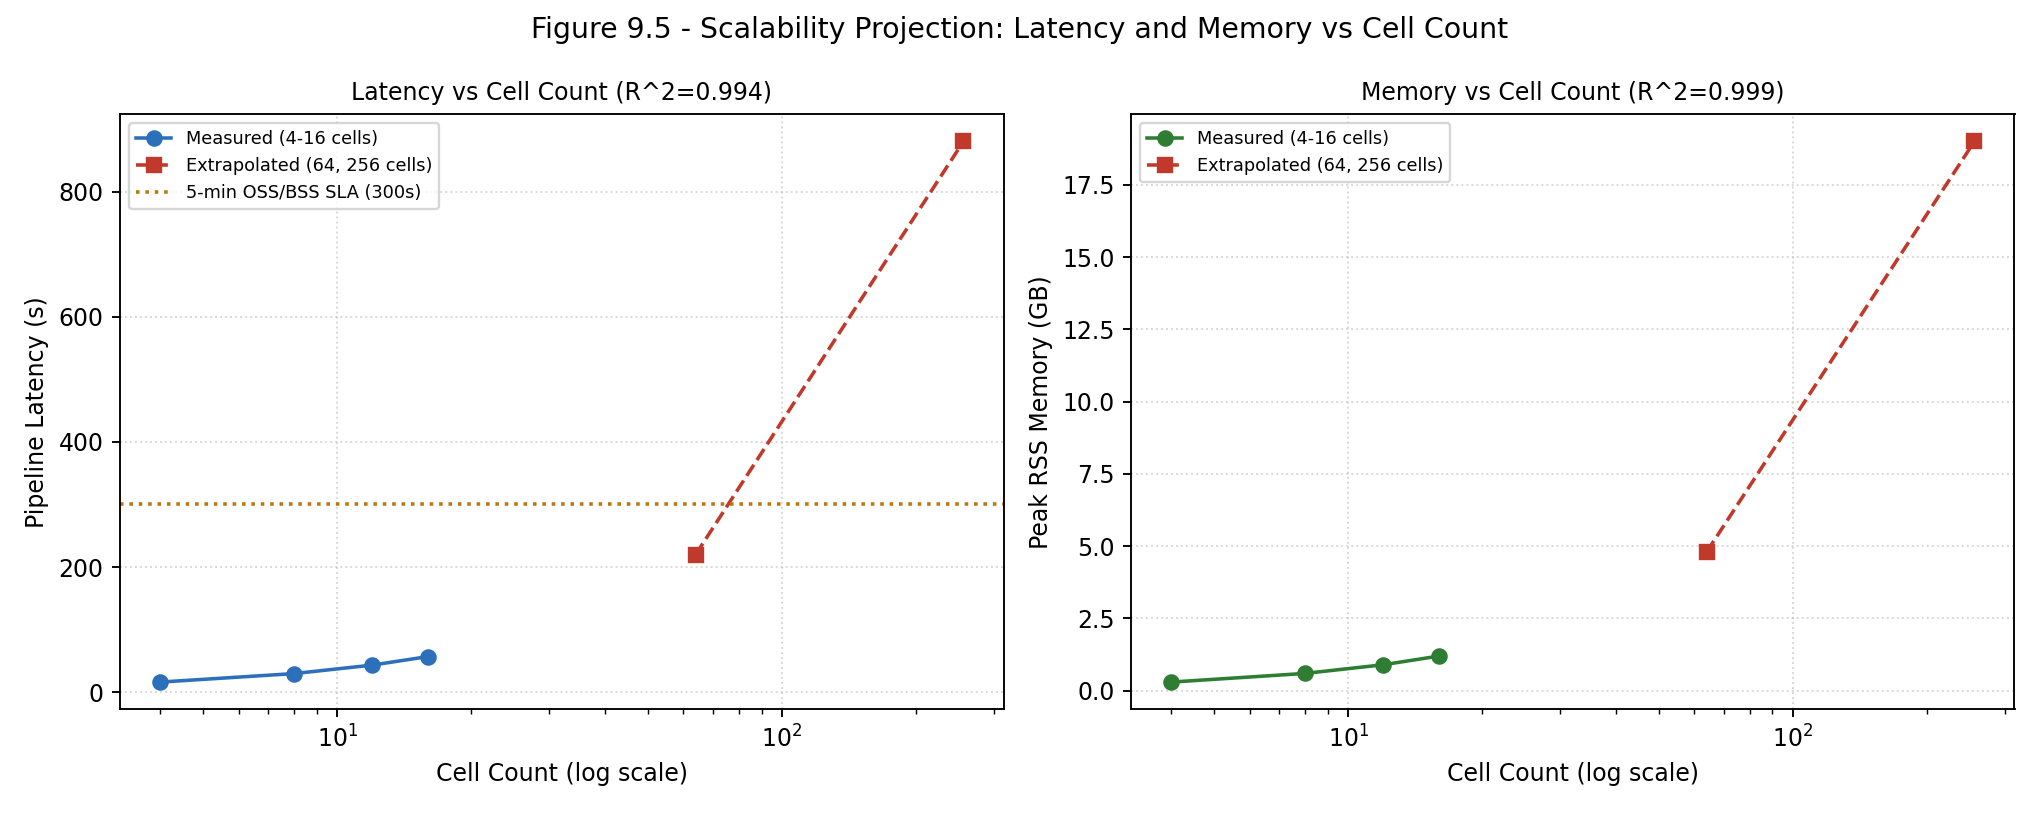
\includegraphics[width=0.85\textwidth]{figures/fig_9_5.png}
    \caption{Scalability Projection (Latency \& Memory vs. Cell Count) --- Measured (4 to 16 cells) and extrapolated (64, 256 cells) pipeline latency and peak memory, with the 5-minute OSS/BSS batch-cycle threshold marked.}
    \label{fig:9_5}
\end{figure}

% ---------------- Chapter 10 ----------------
\begin{figure}[htbp]
    \centering
    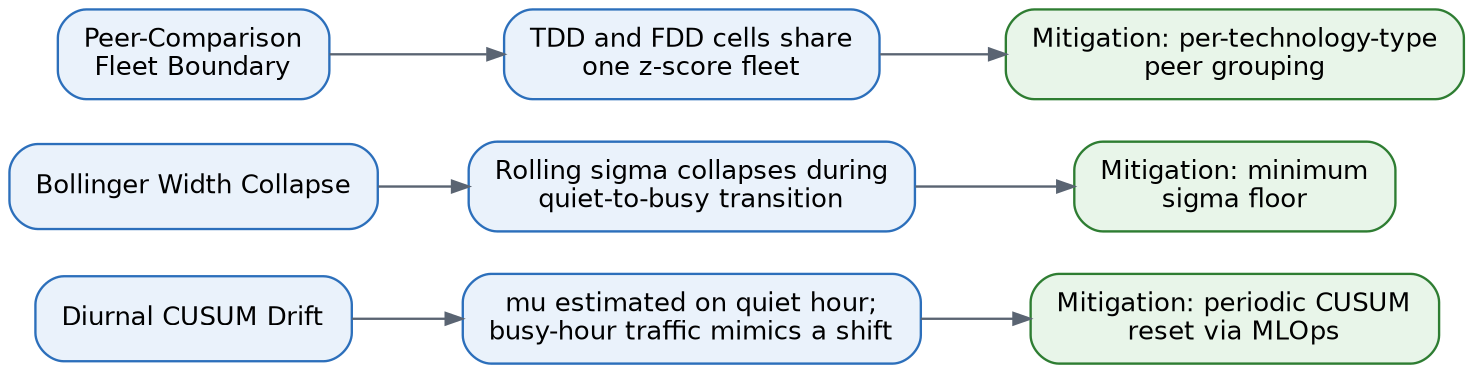
\includegraphics[width=0.85\textwidth]{figures/fig_10_1.png}
    \caption{False-Positive Root-Cause Map --- The three systematic sources of per-record false positives, their underlying mechanism, and the proposed mitigation for each.}
    \label{fig:10_1}
\end{figure}

% ---------------- Chapter 11 ----------------
\begin{figure}[htbp]
    \centering
    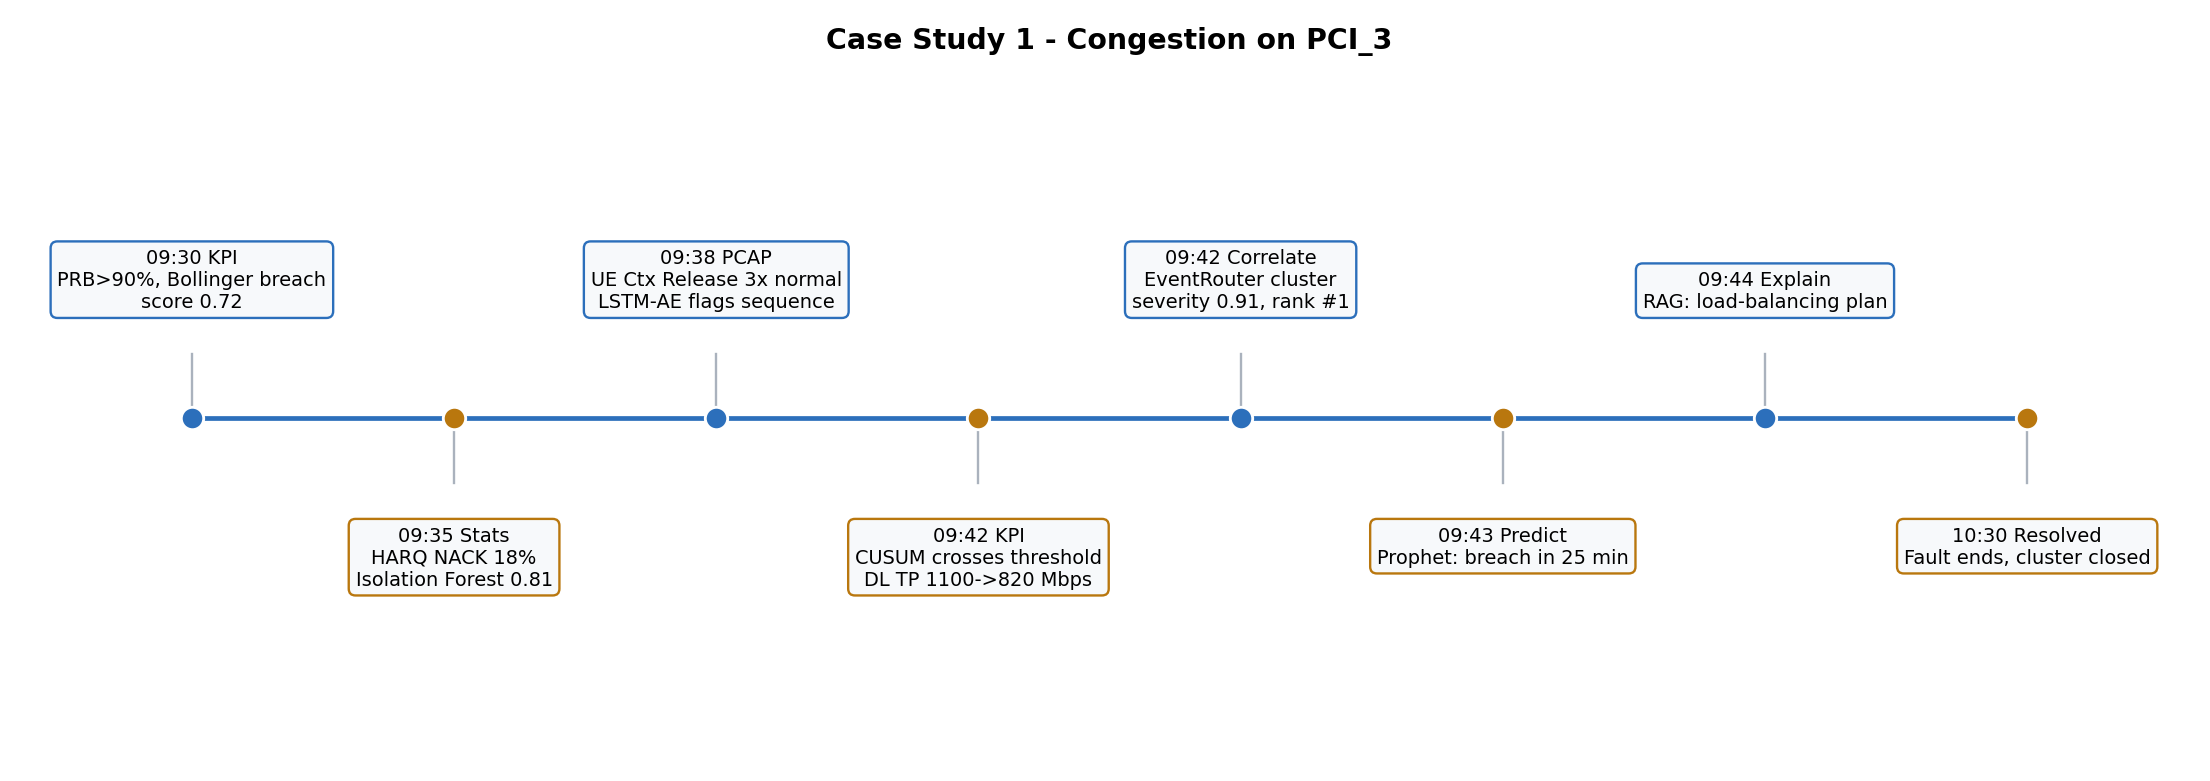
\includegraphics[width=0.85\textwidth]{figures/fig_11_1.png}
    \caption{Case Study 1 Timeline: Congestion on PCI_3 --- End-to-end pipeline trace for the PCI_3 congestion case study, from onset (09:30) to correlated detection (09:42) and explanation (09:44).}
    \label{fig:11_1}
\end{figure}

\begin{figure}[htbp]
    \centering
    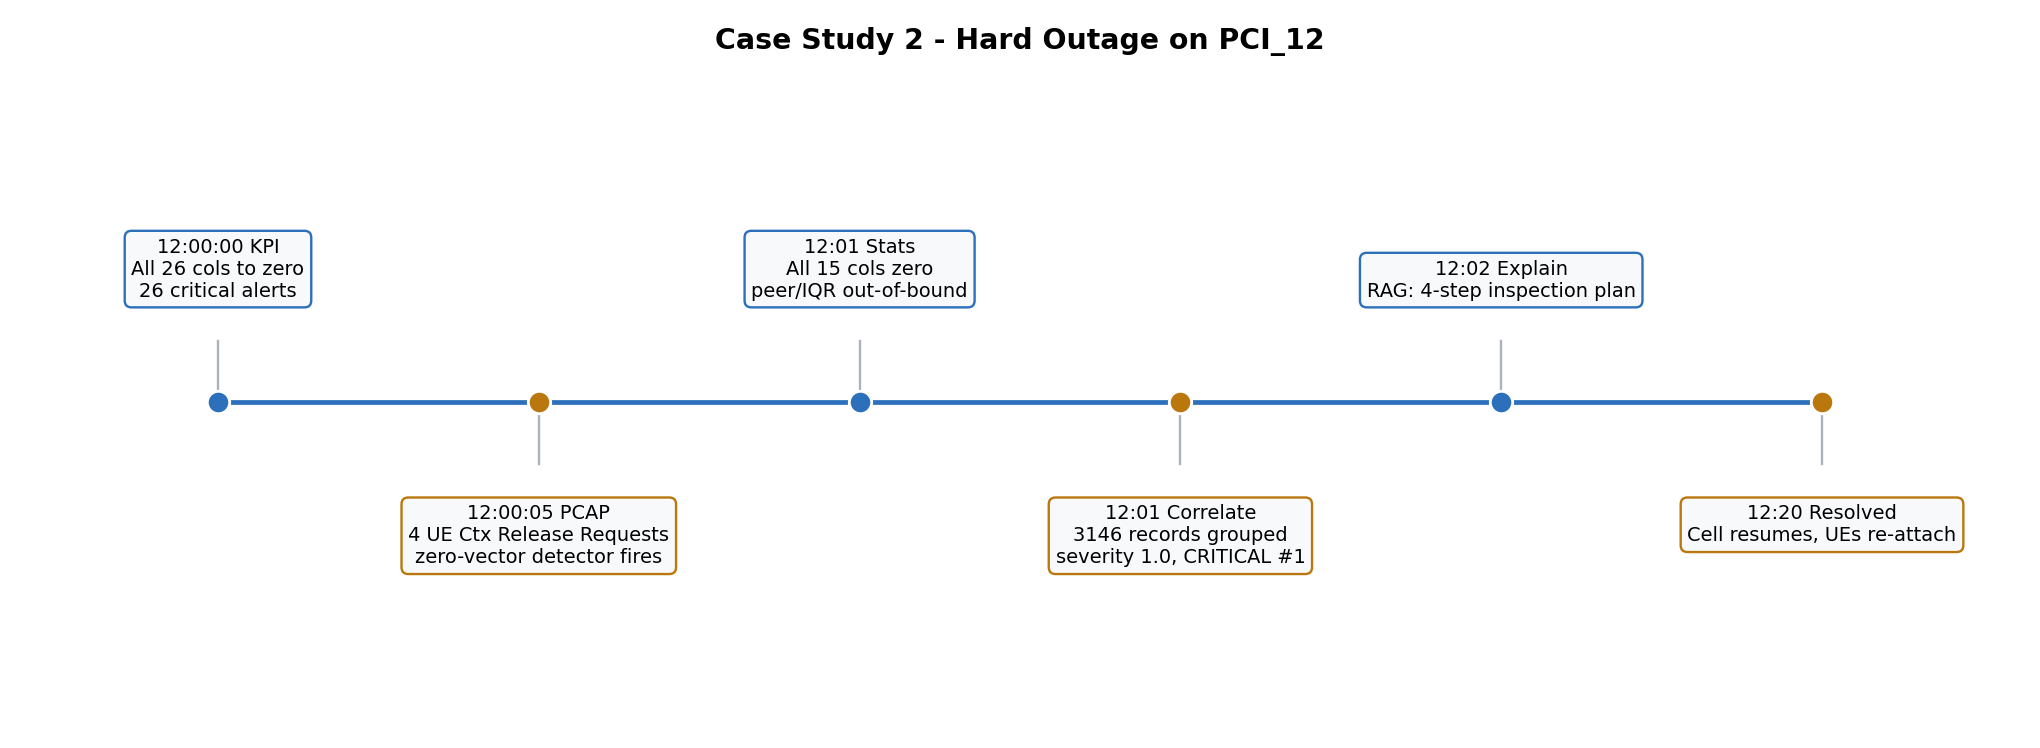
\includegraphics[width=0.85\textwidth]{figures/fig_11_2.png}
    \caption{Case Study 2 Timeline: Hard Outage on PCI_12 --- End-to-end pipeline trace for the PCI_12 hard outage, showing sub-minute detection and immediate severity-1.0 correlation.}
    \label{fig:11_2}
\end{figure}

\begin{figure}[htbp]
    \centering
    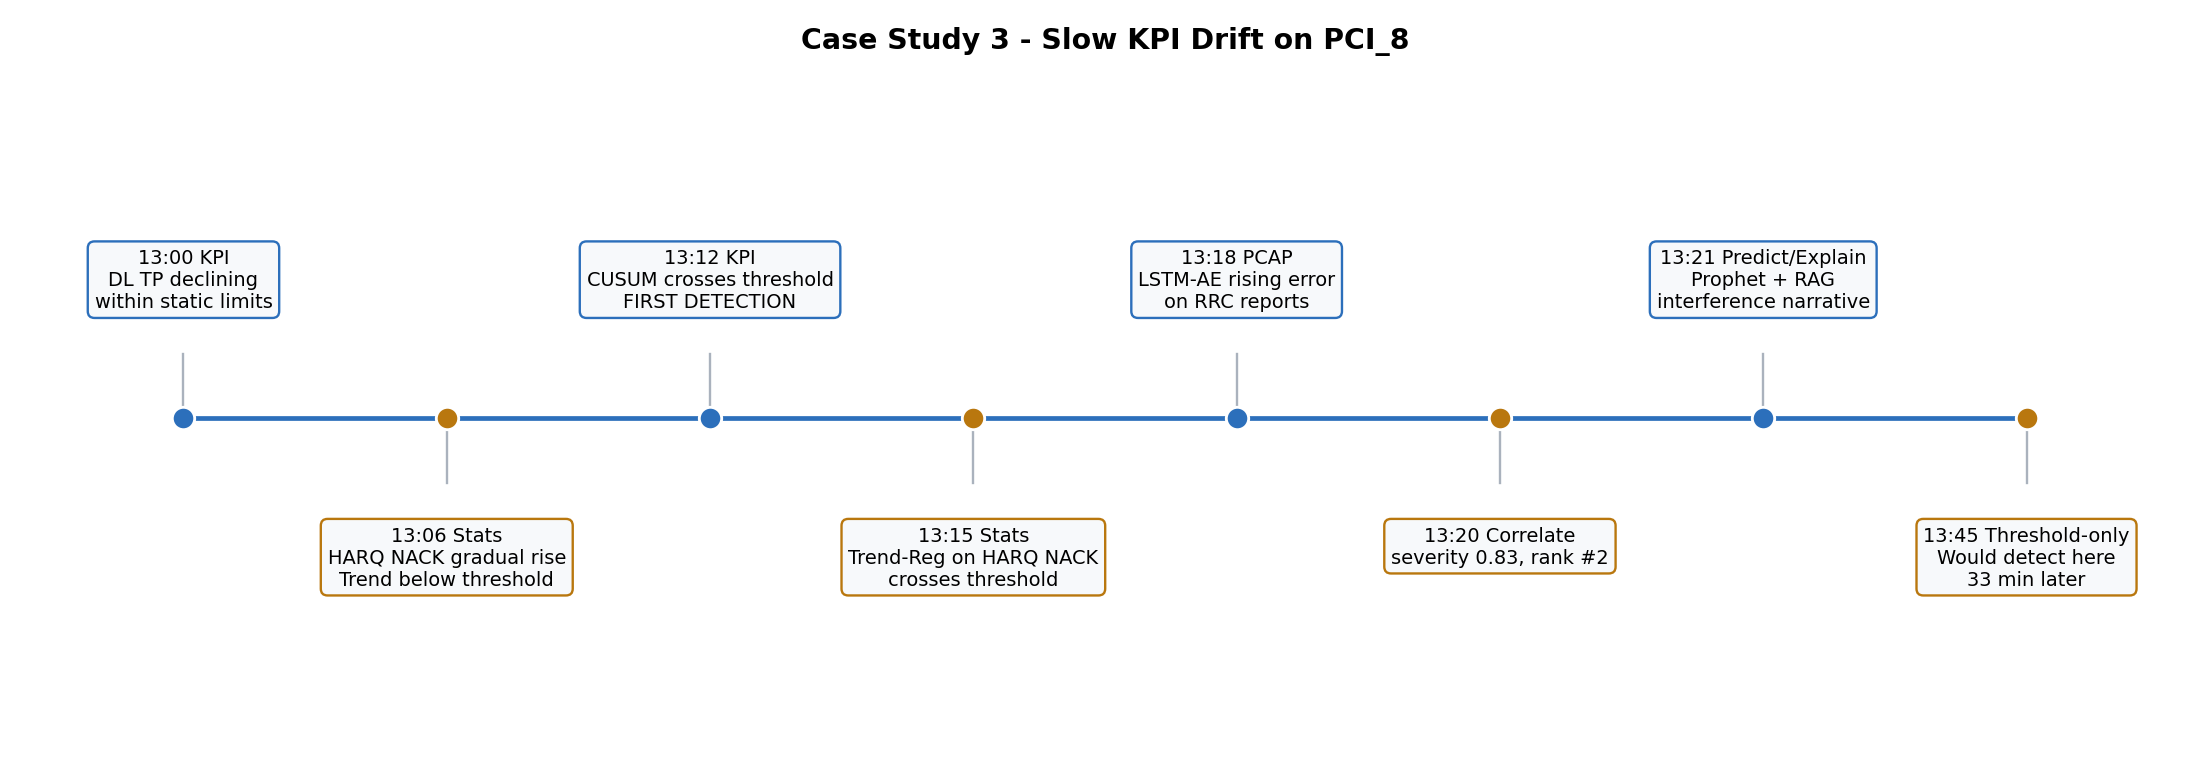
\includegraphics[width=0.85\textwidth]{figures/fig_11_3.png}
    \caption{Case Study 3 Timeline: Slow KPI Drift on PCI_8 --- End-to-end pipeline trace for the PCI_8 slow-drift case study, highlighting the 33-minute early-detection advantage of CUSUM over a threshold-only baseline.}
    \label{fig:11_3}
\end{figure}

% ---------------- Chapter 12 ----------------
\begin{figure}[htbp]
    \centering
    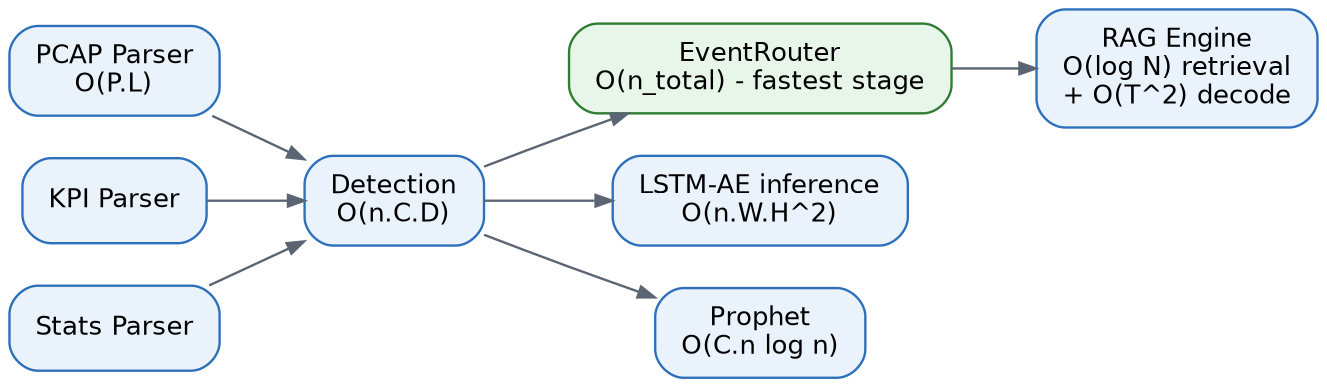
\includegraphics[width=0.85\textwidth]{figures/fig_12_1.png}
    \caption{Module-Level Complexity Overview --- Pipeline stages annotated with their asymptotic time complexity, showing the EventRouter as the fastest stage despite processing the largest input.}
    \label{fig:12_1}
\end{figure}

% ---------------- Chapter 14 ----------------
\begin{figure}[htbp]
    \centering
    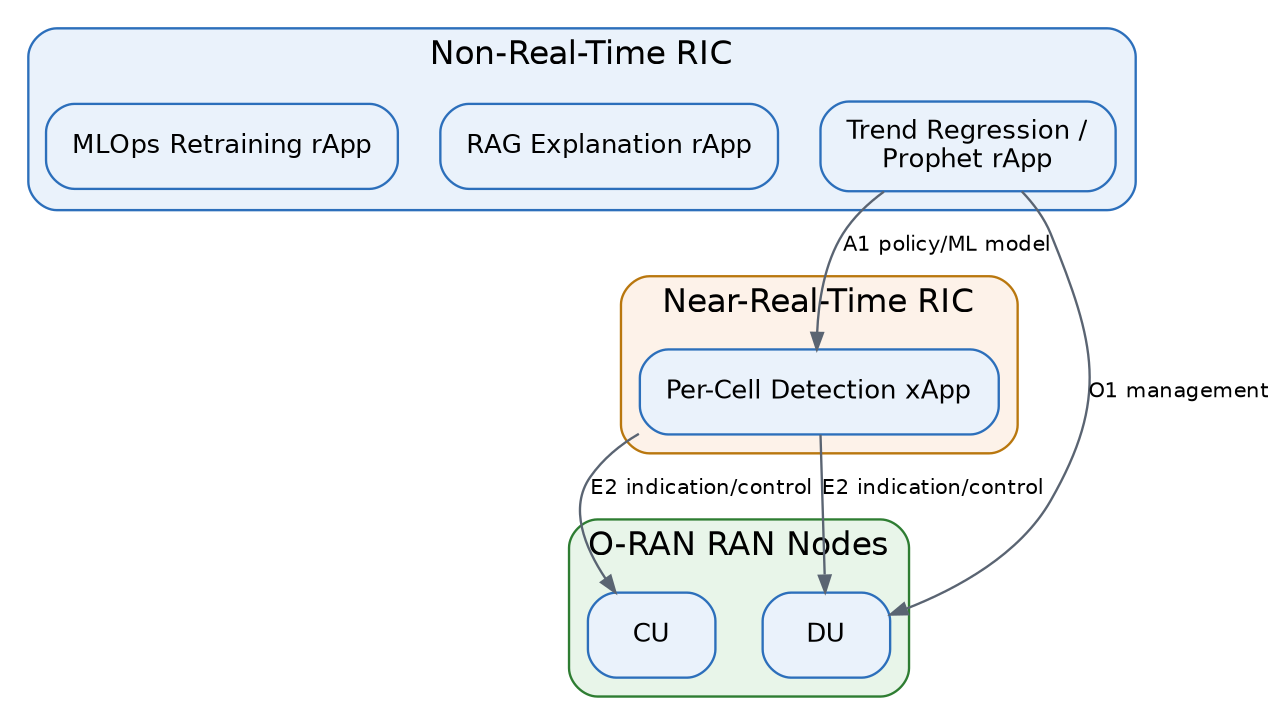
\includegraphics[width=0.85\textwidth]{figures/fig_14_1.png}
    \caption{O-RAN RIC Integration Architecture --- Mapping of the Unified Telecom Analyzer's pipeline modules onto the O-RAN Non-RT RIC (rApps) and Near-RT RIC (xApp) via the A1, O1, and E2 interfaces.}
    \label{fig:14_1}
\end{figure}

\begin{figure}[htbp]
    \centering
    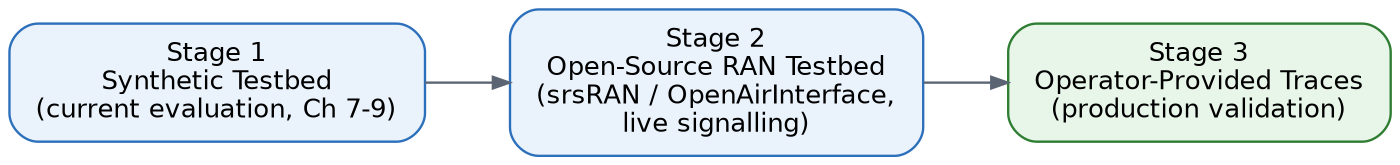
\includegraphics[width=0.85\textwidth]{figures/fig_14_2.png}
    \caption{Staged Production Validation Roadmap --- The staged validation path from the current synthetic evaluation to production deployment on operator traces.}
    \label{fig:14_2}
\end{figure}

\begin{figure}[htbp]
    \centering
    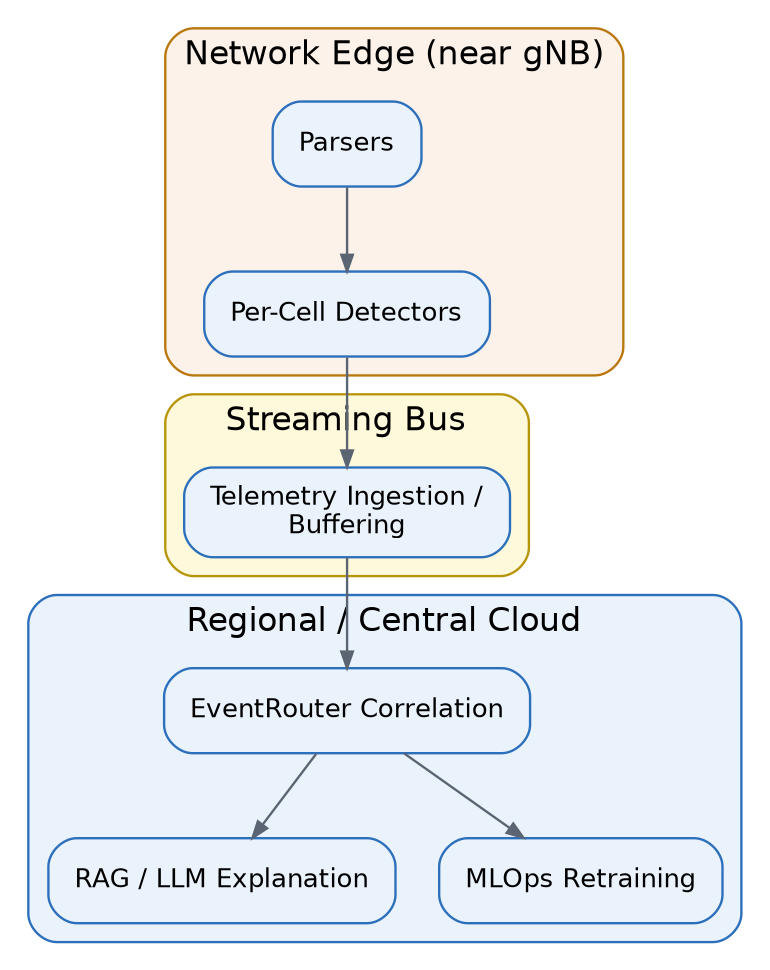
\includegraphics[width=0.85\textwidth]{figures/fig_14_3.png}
    \caption{Cloud-Native Deployment with Edge/Central Split --- Cloud-native deployment topology with latency-sensitive detection at the network edge and heavier RAG/LLM and retraining workloads in central/regional cloud.}
    \label{fig:14_3}
\end{figure}

% ---------------- Chapter 15 ----------------
\begin{figure}[htbp]
    \centering
    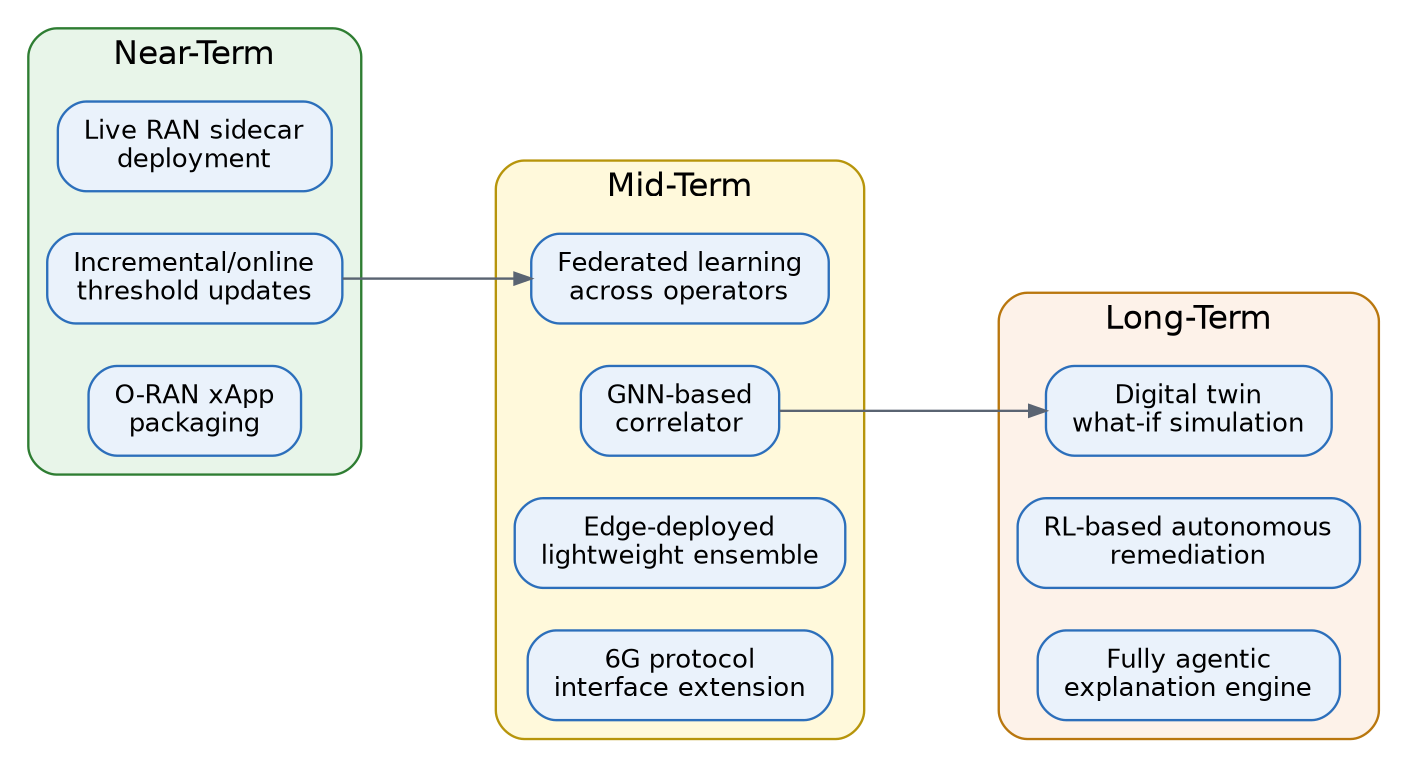
\includegraphics[width=0.85\textwidth]{figures/fig_15_1.png}
    \caption{Future Work Roadmap (Near-Term to Long-Term) --- The ten future work directions grouped by implementation horizon, from near-term engineering extensions to long-term autonomous-network research.}
    \label{fig:15_1}
\end{figure}

% ---------------- Chapter A ----------------
\begin{figure}[htbp]
    \centering
    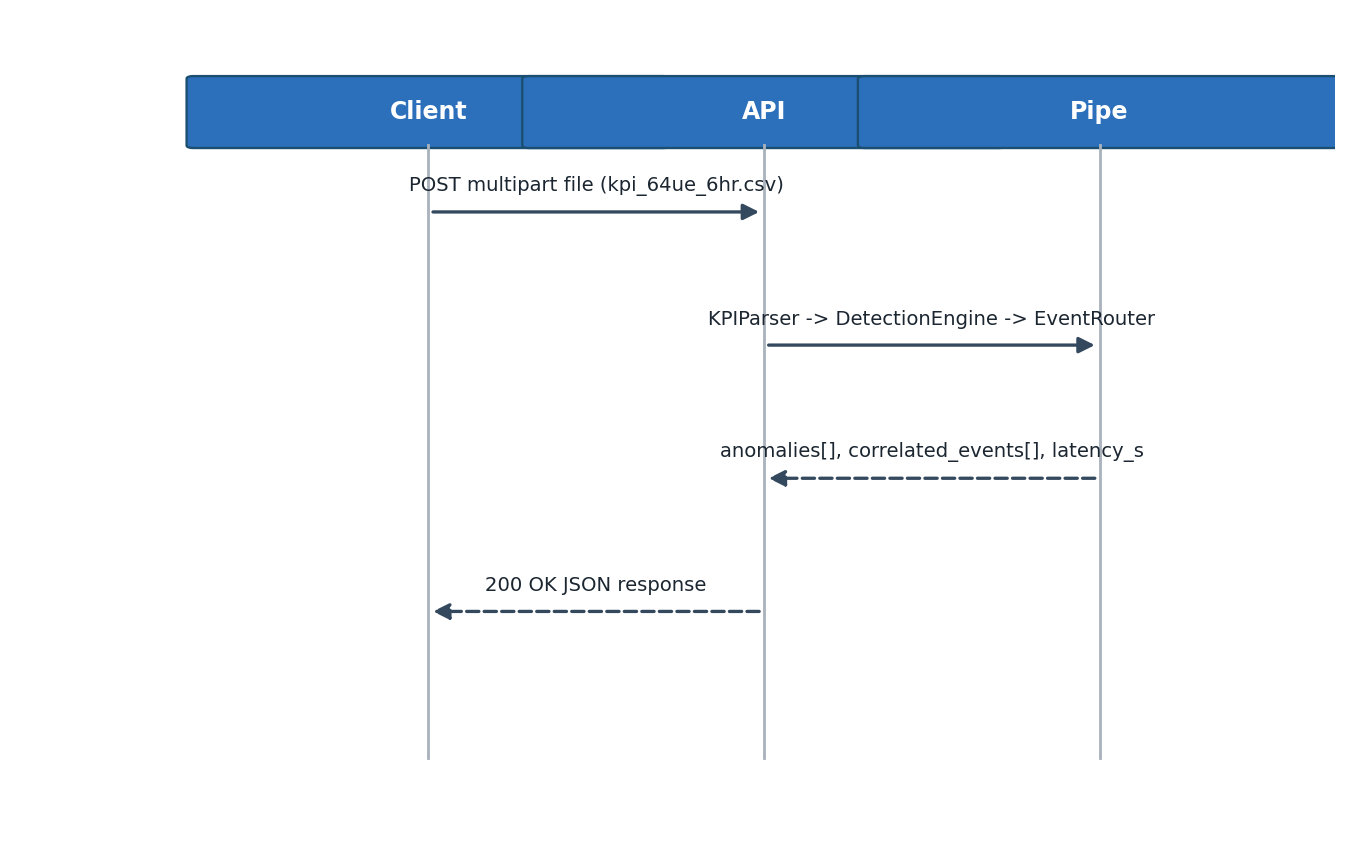
\includegraphics[width=0.85\textwidth]{figures/fig_A_1.png}
    \caption{Sample API Request/Response Flow --- Request/response sequence for the POST /analyze/kpi endpoint, from file upload through pipeline execution to JSON response.}
    \label{fig:A_1}
\end{figure}
  (place after \usepackage{graphicx})
% All images are in the figures/ subfolder - upload that folder to your Overleaf project root.
% ===================================================================

% ---------------- Chapter 1 ----------------
\begin{figure}[htbp]
    \centering
    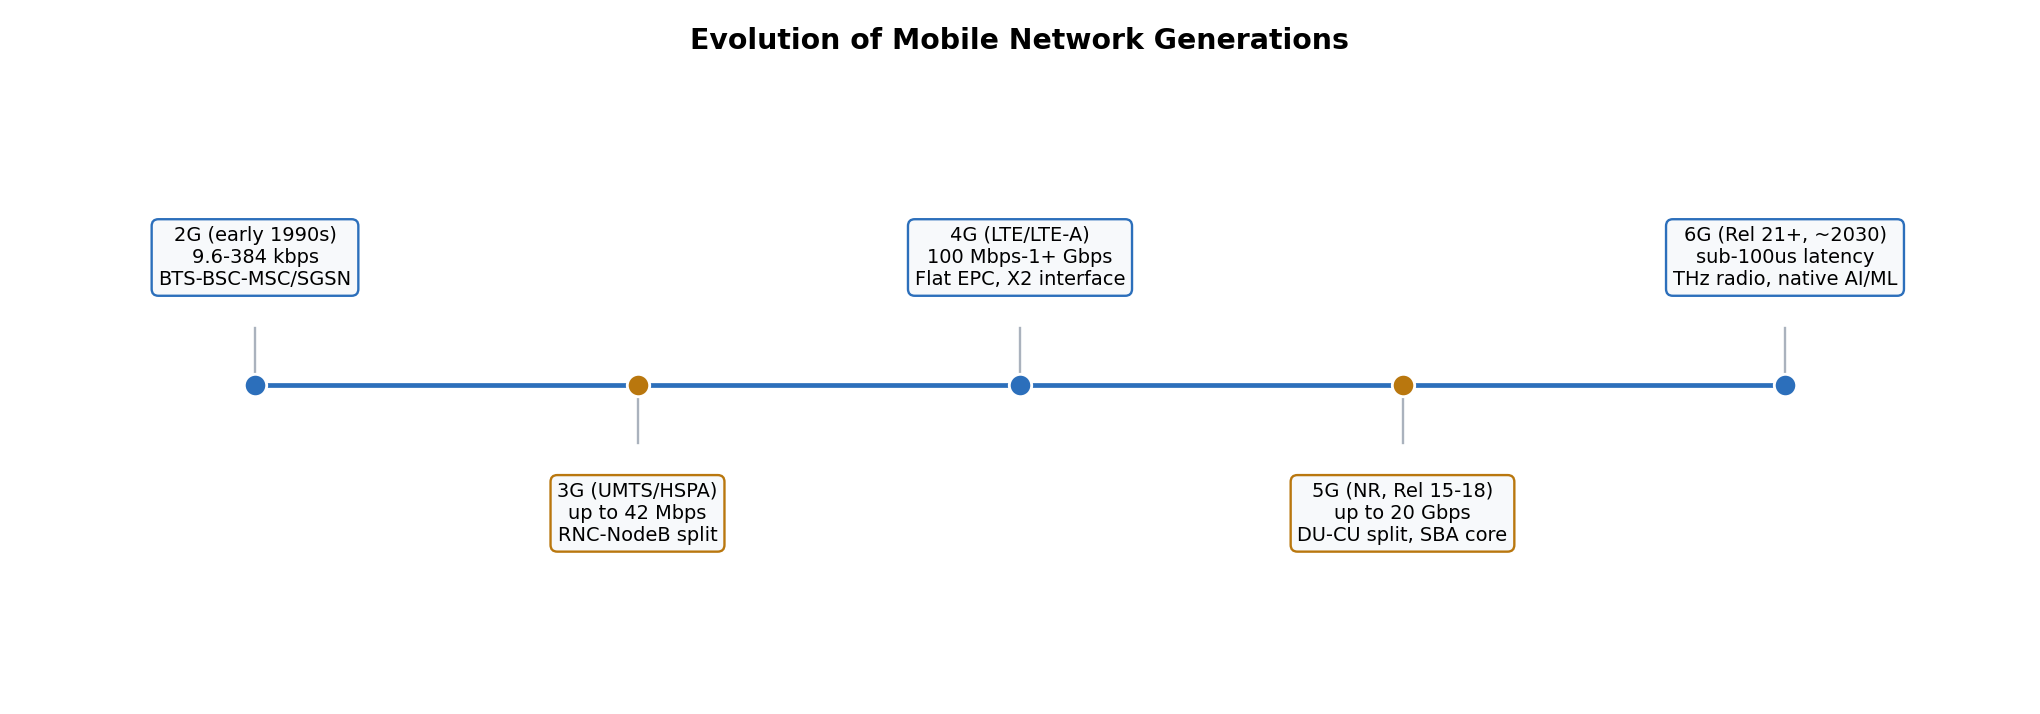
\includegraphics[width=0.85\textwidth]{figures/fig_1_1.png}
    \caption{Evolution of Mobile Network Generations --- Evolution of mobile network generations from 2G to the envisioned 6G, showing peak data rate and defining architectural change at each step.}
    \label{fig:1_1}
\end{figure}

\begin{figure}[htbp]
    \centering
    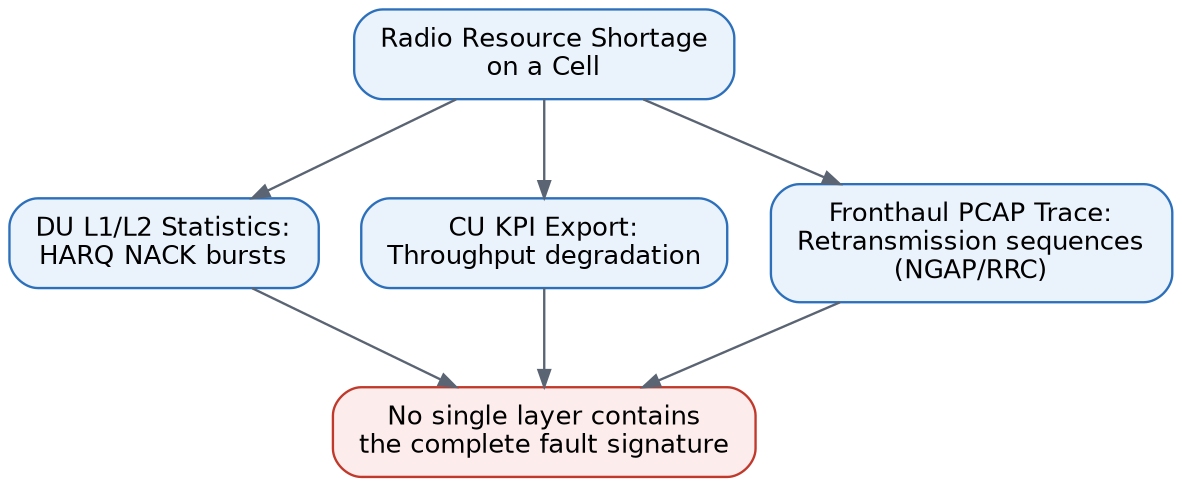
\includegraphics[width=0.85\textwidth]{figures/fig_1_2.png}
    \caption{Multi-Layer Fault Signature Propagation --- A single radio-resource fault propagates distinct, incomplete signatures into each of the three telemetry domains, motivating multi-modal detection.}
    \label{fig:1_2}
\end{figure}

\begin{figure}[htbp]
    \centering
    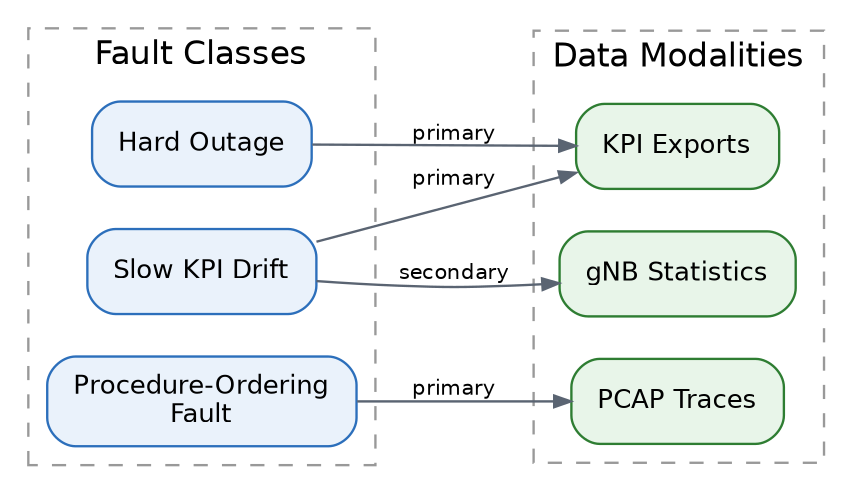
\includegraphics[width=0.85\textwidth]{figures/fig_1_3.png}
    \caption{Complementary Fault Coverage of the Three Modalities --- Mapping of the three targeted fault classes to their primary detecting modality, illustrating why no single data source covers the full fault taxonomy.}
    \label{fig:1_3}
\end{figure}

% ---------------- Chapter 2 ----------------
\begin{figure}[htbp]
    \centering
    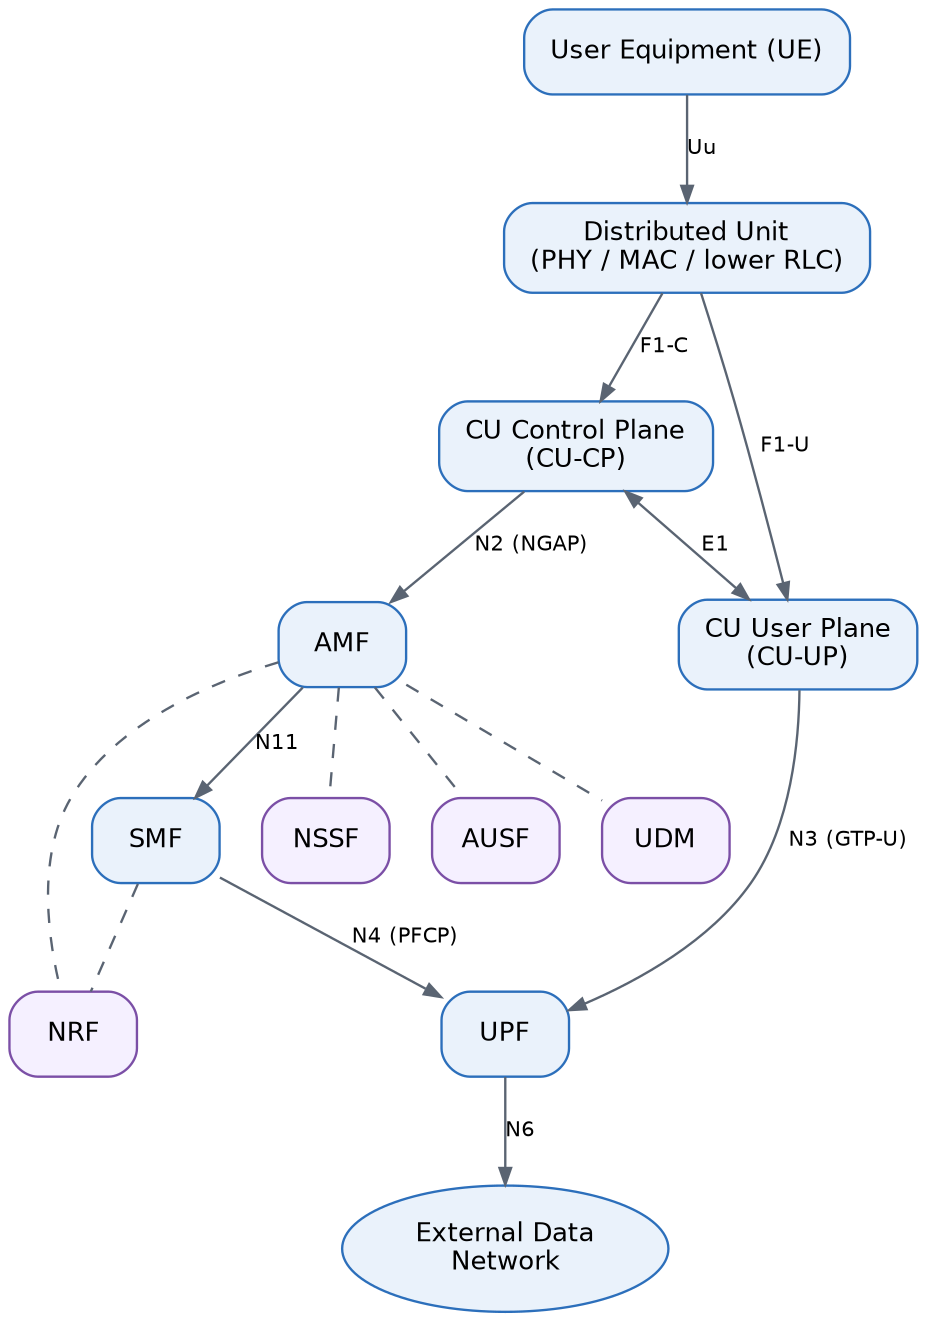
\includegraphics[width=0.85\textwidth]{figures/fig_2_1.png}
    \caption{5G Network Architecture (NG-RAN + 5GC) --- 5G system architecture showing the disaggregated NG-RAN (DU/CU-CP/CU-UP) and the Service-Based Architecture of the 5G Core.}
    \label{fig:2_1}
\end{figure}

\begin{figure}[htbp]
    \centering
    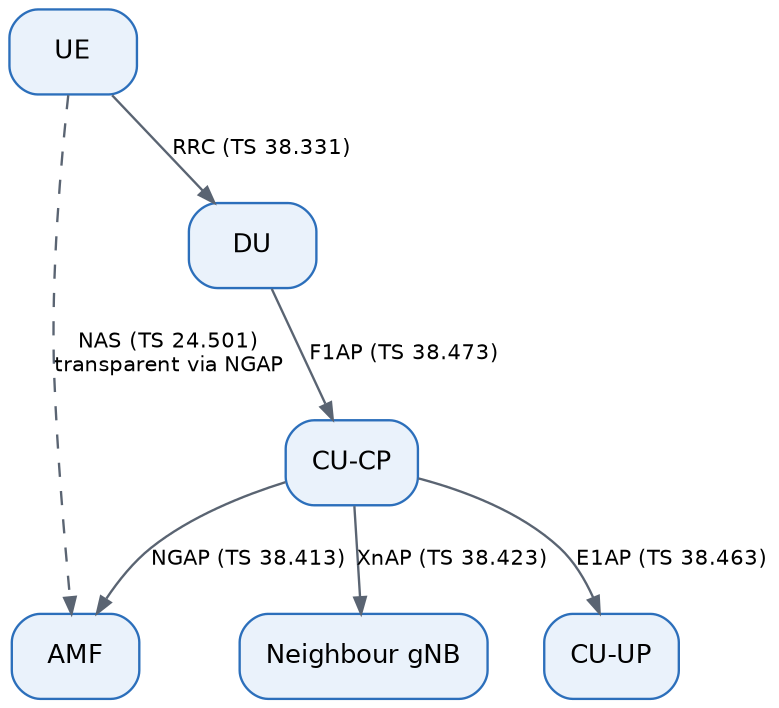
\includegraphics[width=0.85\textwidth]{figures/fig_2_2.png}
    \caption{Six Protocol Interfaces Mapped to Network Nodes --- The six 5G-NR protocol interfaces parsed by the PCAP Parser, mapped to their governing 3GPP specification and network-node endpoints.}
    \label{fig:2_2}
\end{figure}

% ---------------- Chapter 3 ----------------
\begin{figure}[htbp]
    \centering
    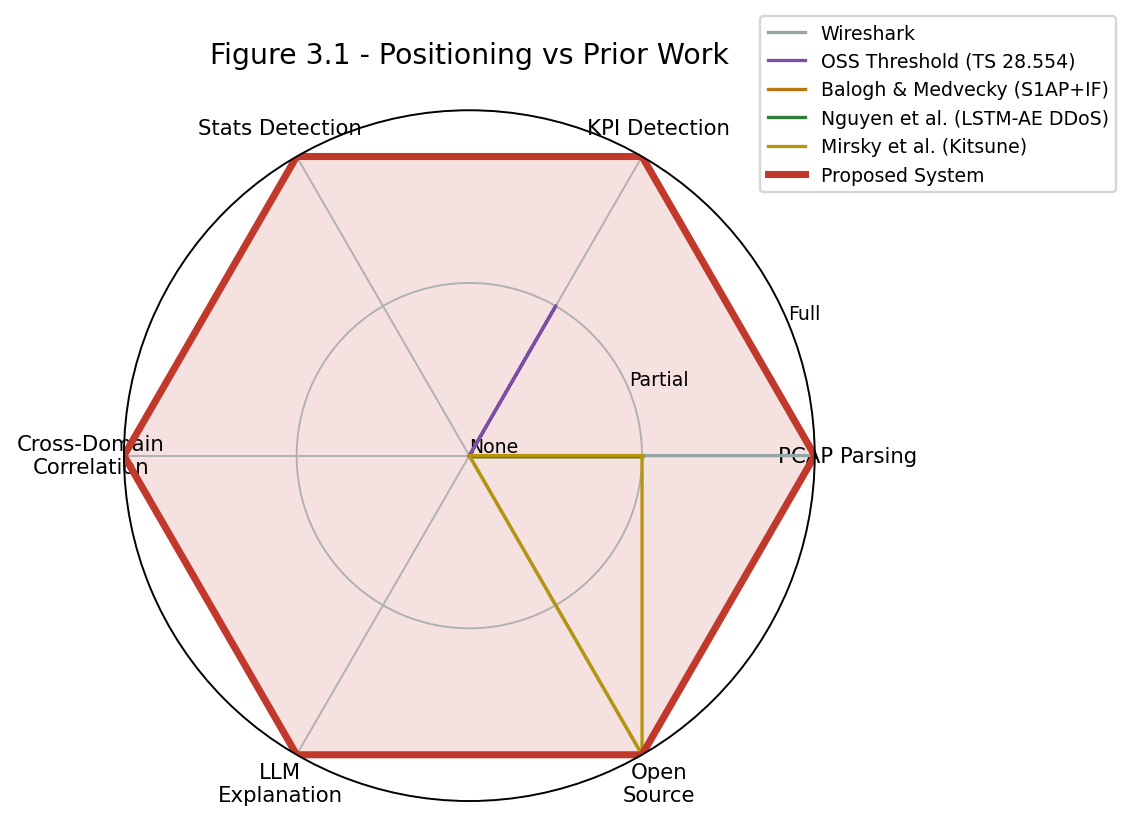
\includegraphics[width=0.85\textwidth]{figures/fig_3_1.png}
    \caption{Positioning Comparison vs. Prior Work --- Radar comparison of the proposed system against five representative prior systems across the five positioning axes of Table 3.1.}
    \label{fig:3_1}
\end{figure}

% ---------------- Chapter 4 ----------------
\begin{figure}[htbp]
    \centering
    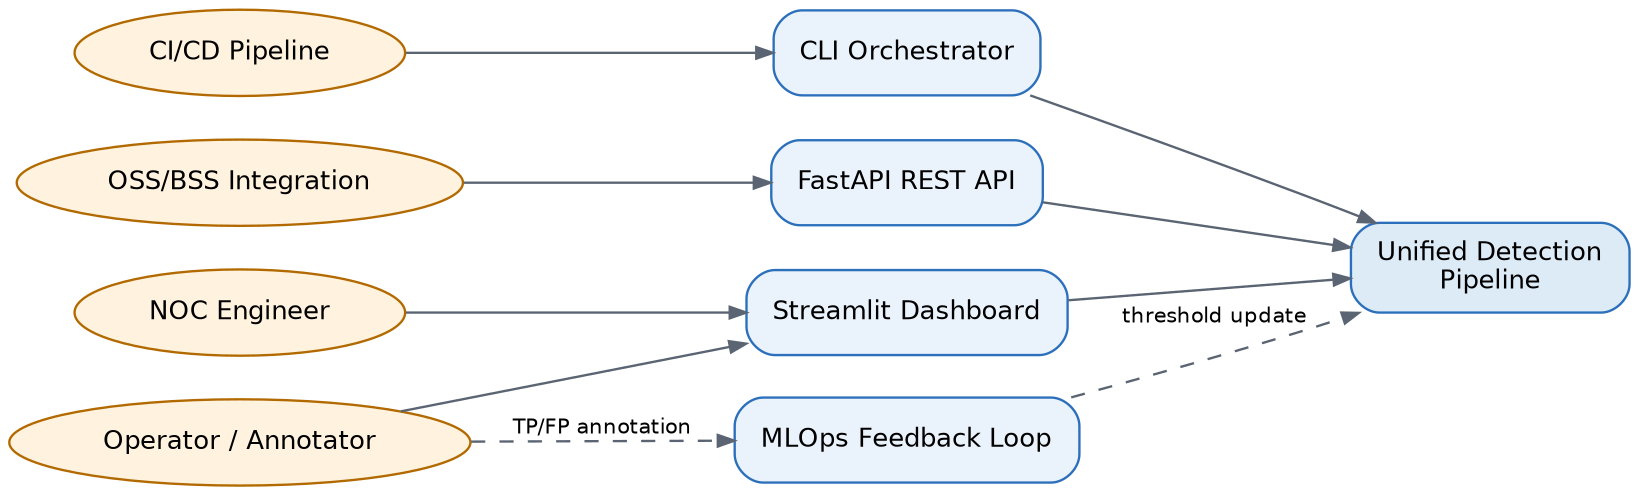
\includegraphics[width=0.85\textwidth]{figures/fig_4_1.png}
    \caption{Use Case Diagram --- Actors and access interfaces for the Unified Telecom Analyzer, tracing each functional requirement to its consuming role.}
    \label{fig:4_1}
\end{figure}

% ---------------- Chapter 5 ----------------
\begin{figure}[htbp]
    \centering
    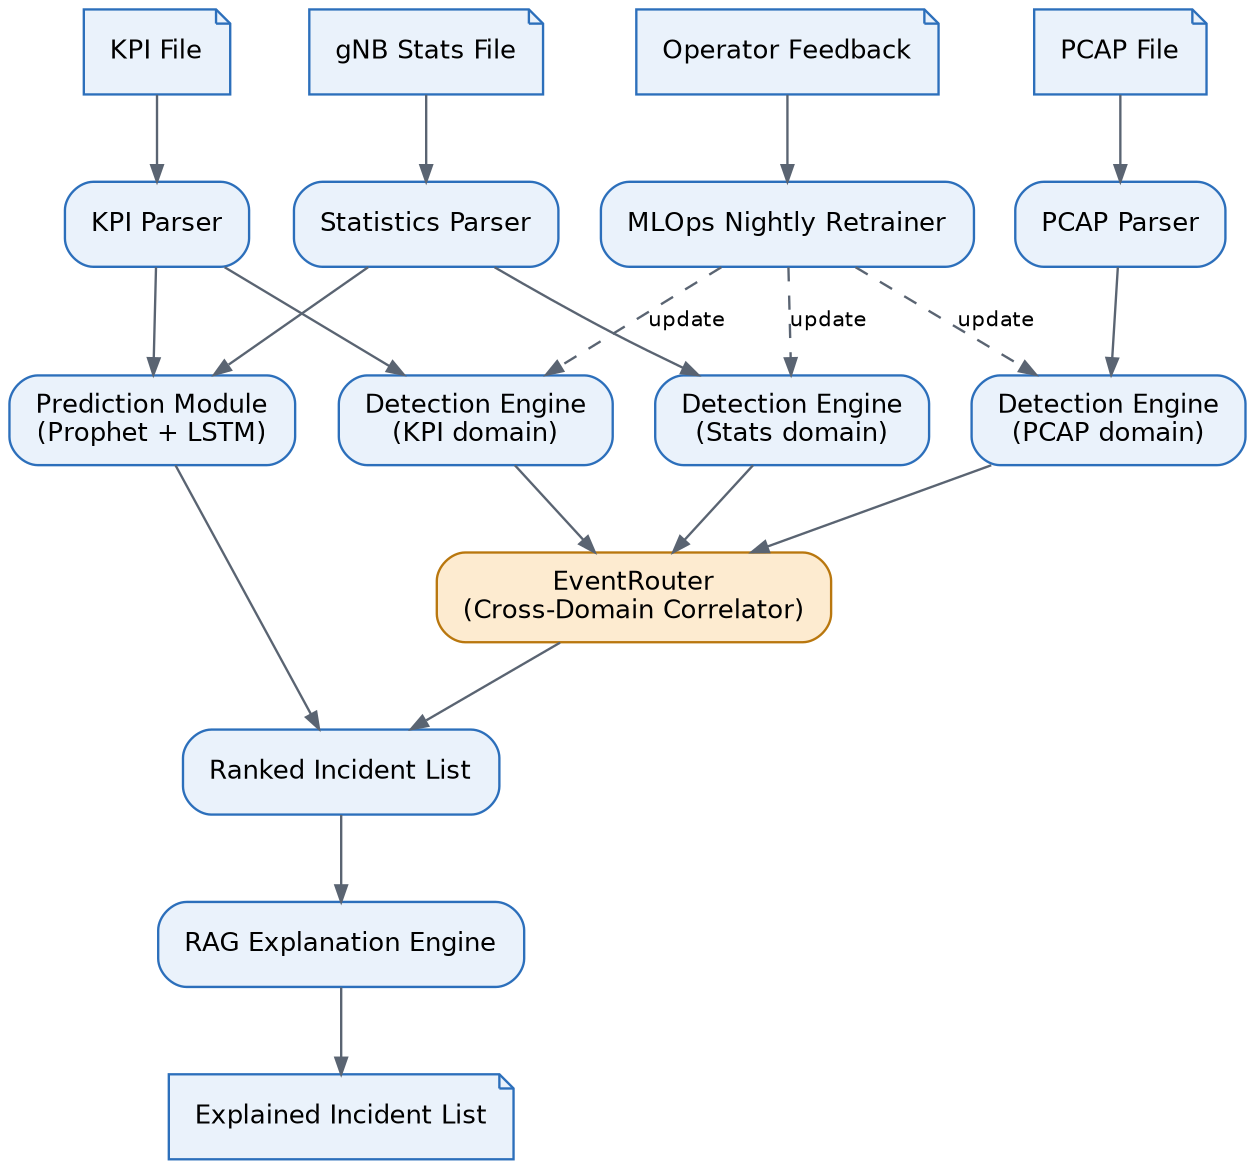
\includegraphics[width=0.85\textwidth]{figures/fig_5_1.png}
    \caption{Unified Pipeline End-to-End Control Flow --- End-to-end control flow of the Unified Telecom Analyzer, showing the Parse to Detect to Correlate to Explain pipeline with parallel Prediction and MLOps feedback branches.}
    \label{fig:5_1}
\end{figure}

\begin{figure}[htbp]
    \centering
    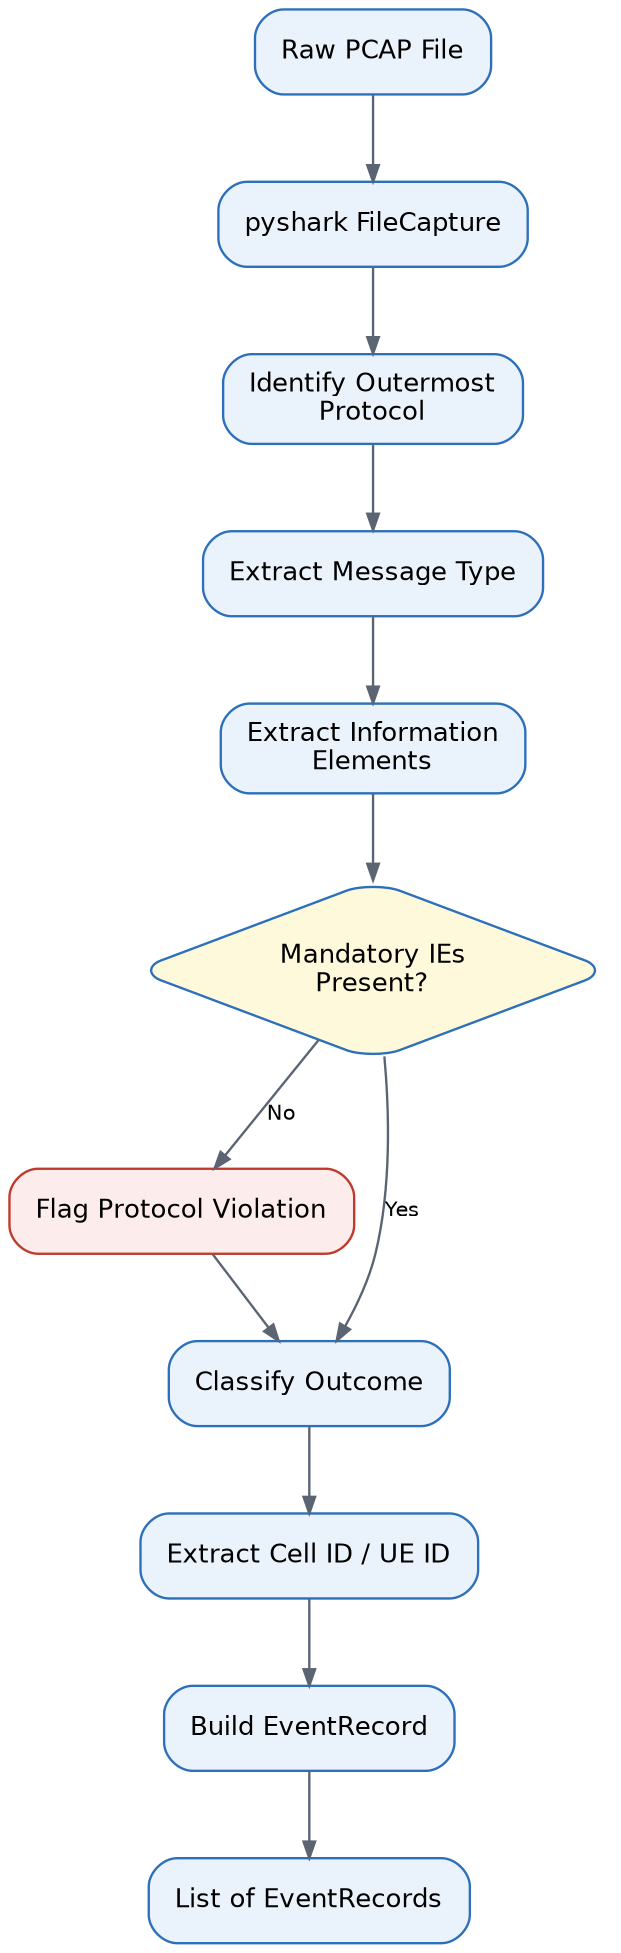
\includegraphics[width=0.85\textwidth]{figures/fig_5_2.png}
    \caption{PCAP Parser Workflow --- PCAP Parser processing workflow, including the spec-alignment branch that flags protocol violations independently of the anomaly ensemble.}
    \label{fig:5_2}
\end{figure}

\begin{figure}[htbp]
    \centering
    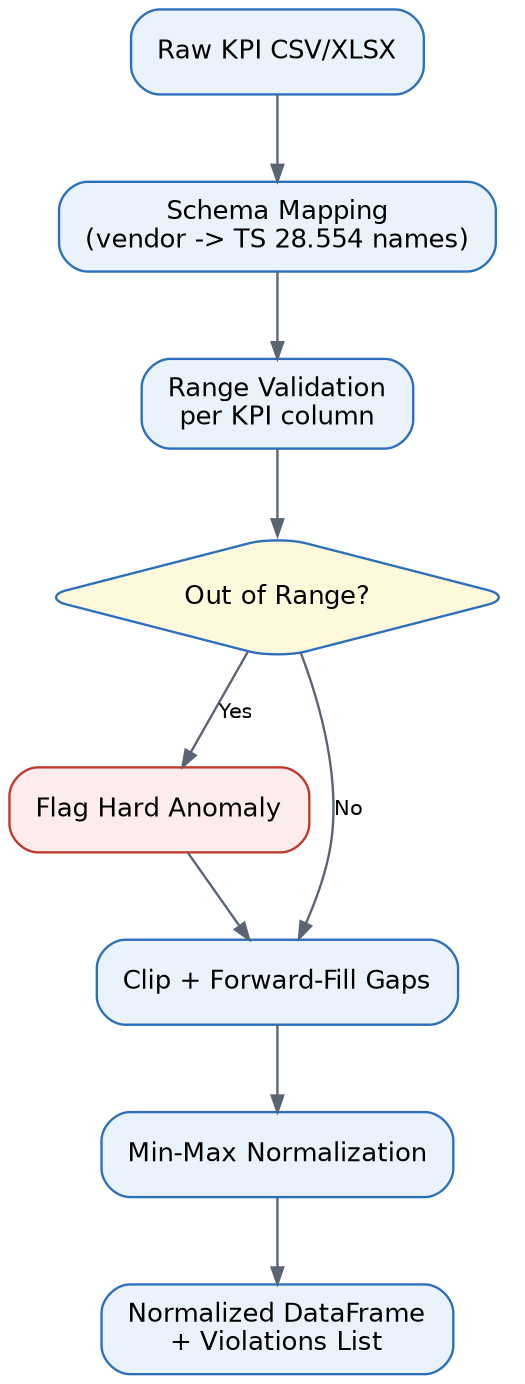
\includegraphics[width=0.85\textwidth]{figures/fig_5_3.png}
    \caption{KPI Parser Three-Stage Pipeline --- KPI Parser three-stage processing pipeline: schema mapping, range validation, and normalization.}
    \label{fig:5_3}
\end{figure}

\begin{figure}[htbp]
    \centering
    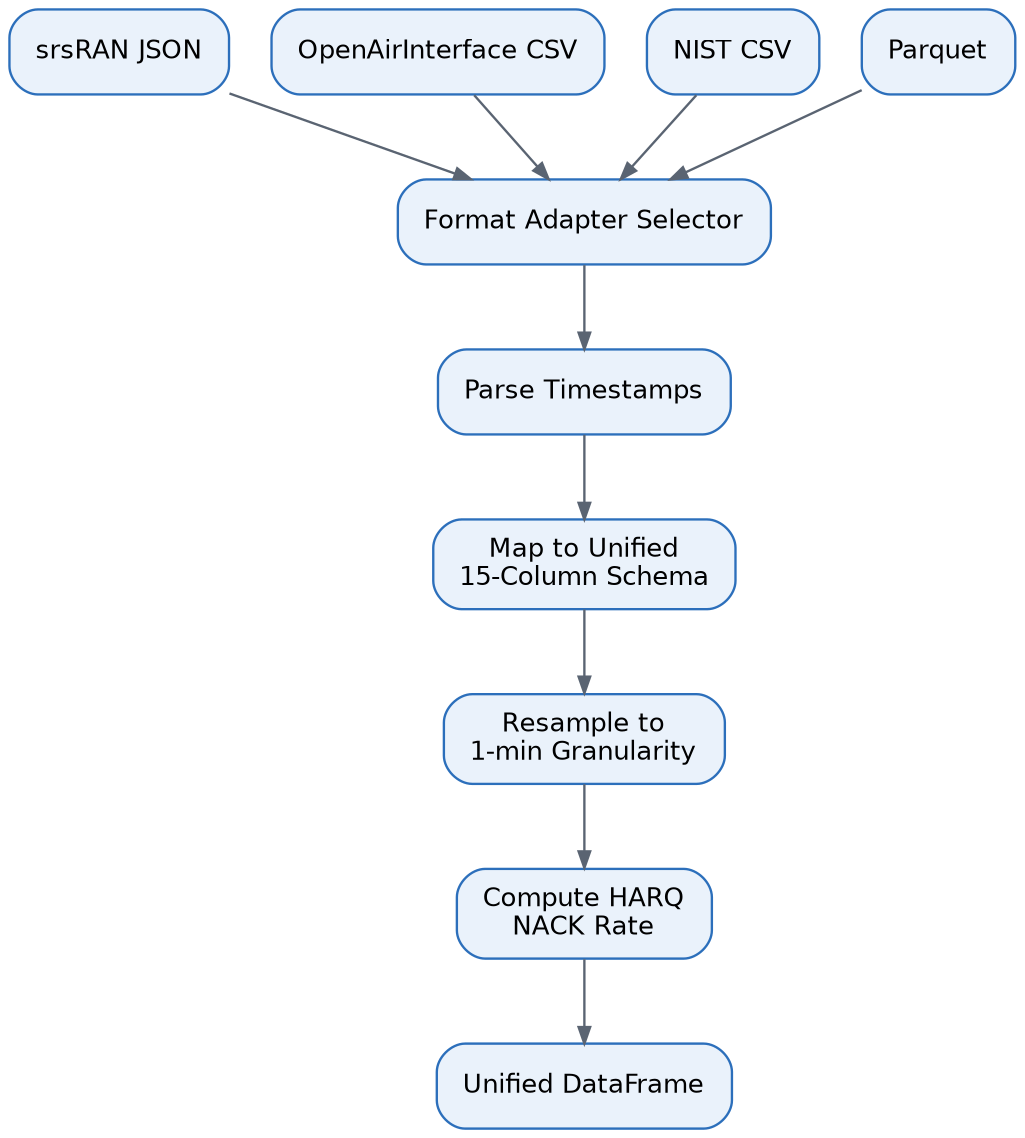
\includegraphics[width=0.85\textwidth]{figures/fig_5_4.png}
    \caption{Statistics Parser Multi-Format Adapter Architecture --- Statistics Parser adapter architecture unifying four input formats into a single 15-column schema.}
    \label{fig:5_4}
\end{figure}

\begin{figure}[htbp]
    \centering
    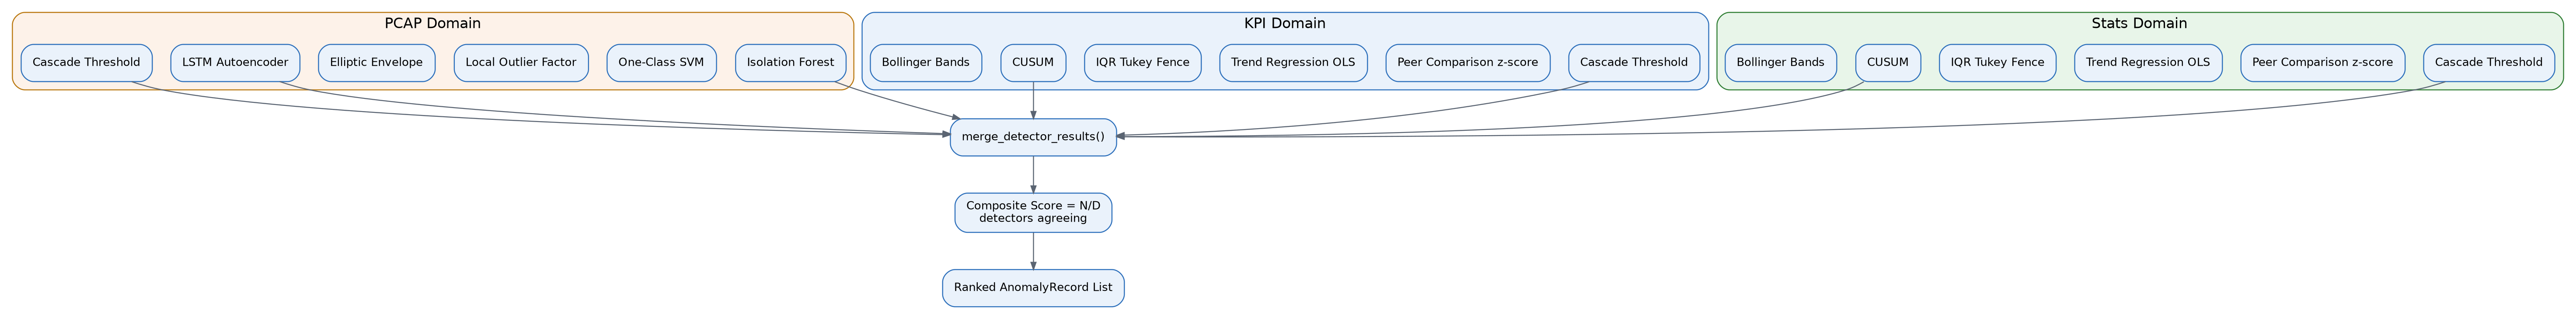
\includegraphics[width=0.85\textwidth]{figures/fig_5_5.png}
    \caption{18-Detector Ensemble Architecture --- 18-detector ensemble architecture: six algorithm families instantiated across three data domains, merged into a composite severity score.}
    \label{fig:5_5}
\end{figure}

\begin{figure}[htbp]
    \centering
    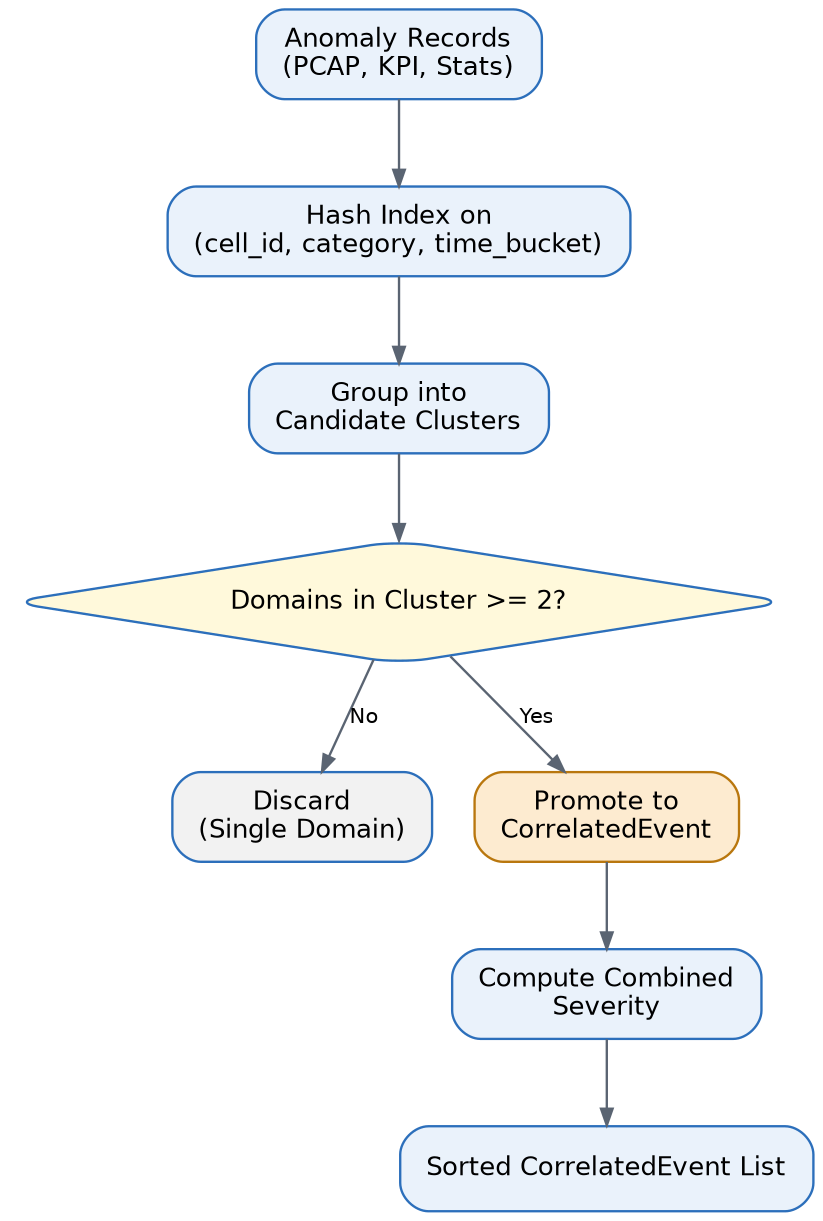
\includegraphics[width=0.85\textwidth]{figures/fig_5_6.png}
    \caption{EventRouter Cross-Domain Correlation --- EventRouter cross-domain correlation mechanism, promoting multi-domain anomaly clusters to CorrelatedEvents.}
    \label{fig:5_6}
\end{figure}

\begin{figure}[htbp]
    \centering
    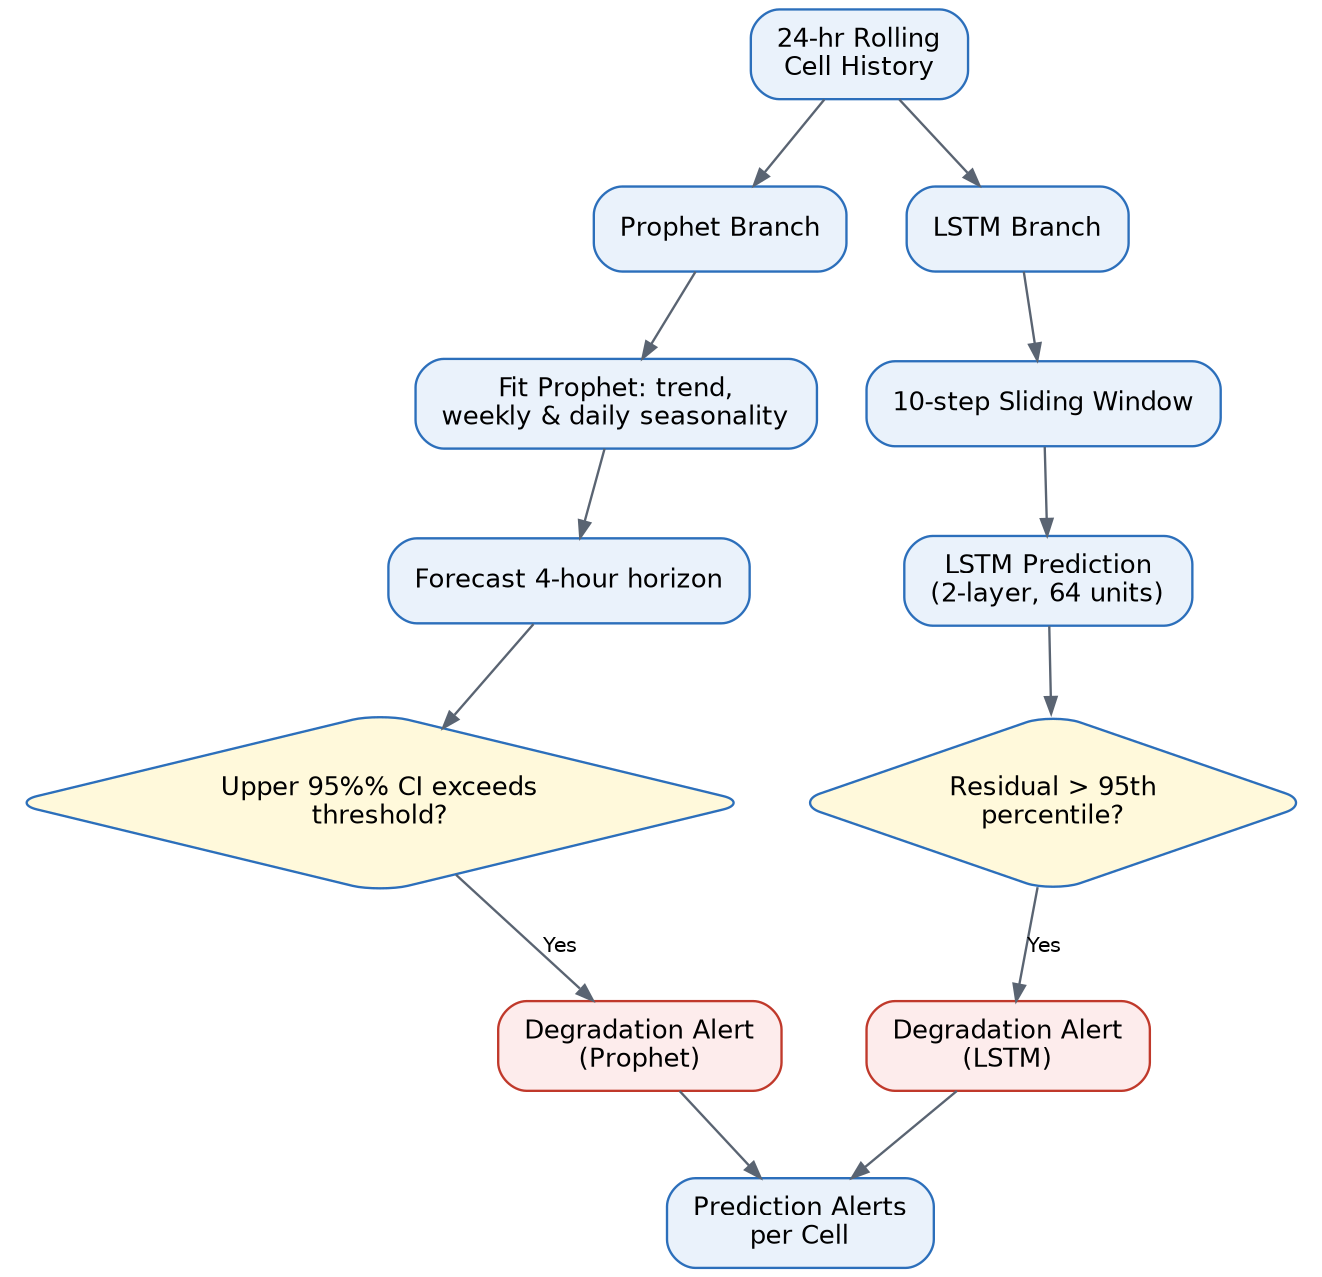
\includegraphics[width=0.85\textwidth]{figures/fig_5_7.png}
    \caption{Prediction Module Dual-Branch Design --- Dual-branch Prediction Module combining Prophet (seasonal patterns) and LSTM (non-linear sudden onset).}
    \label{fig:5_7}
\end{figure}

\begin{figure}[htbp]
    \centering
    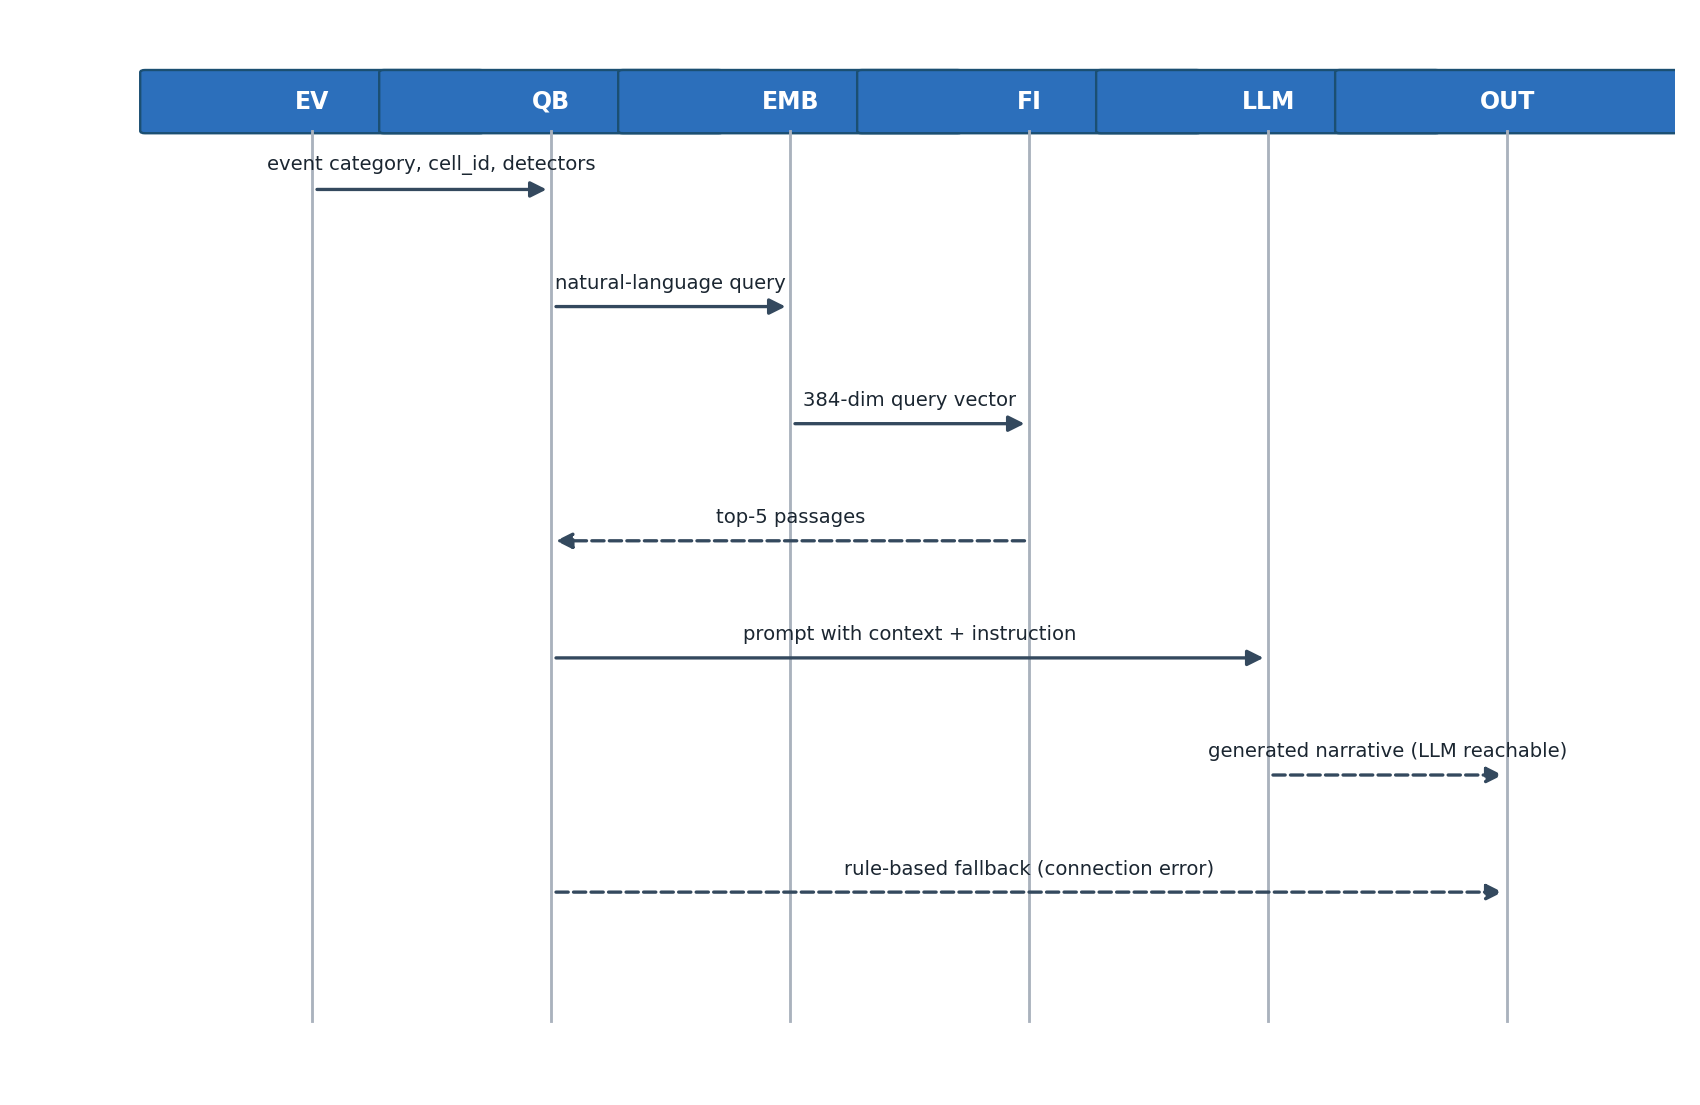
\includegraphics[width=0.85\textwidth]{figures/fig_5_8.png}
    \caption{RAG Explanation Engine Flow --- RAG Explanation Engine pipeline: query construction, FAISS retrieval, and LLM generation with offline fallback.}
    \label{fig:5_8}
\end{figure}

\begin{figure}[htbp]
    \centering
    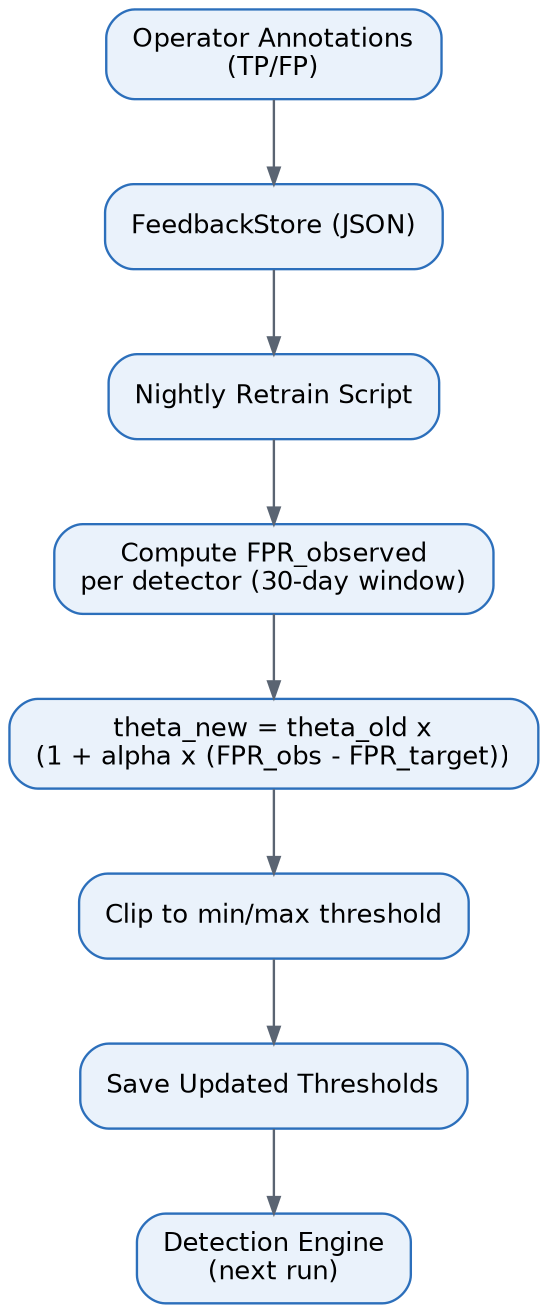
\includegraphics[width=0.85\textwidth]{figures/fig_5_9.png}
    \caption{MLOps Nightly Feedback Loop --- MLOps nightly feedback loop adjusting per-detector thresholds from operator false-positive annotations.}
    \label{fig:5_9}
\end{figure}

\begin{figure}[htbp]
    \centering
    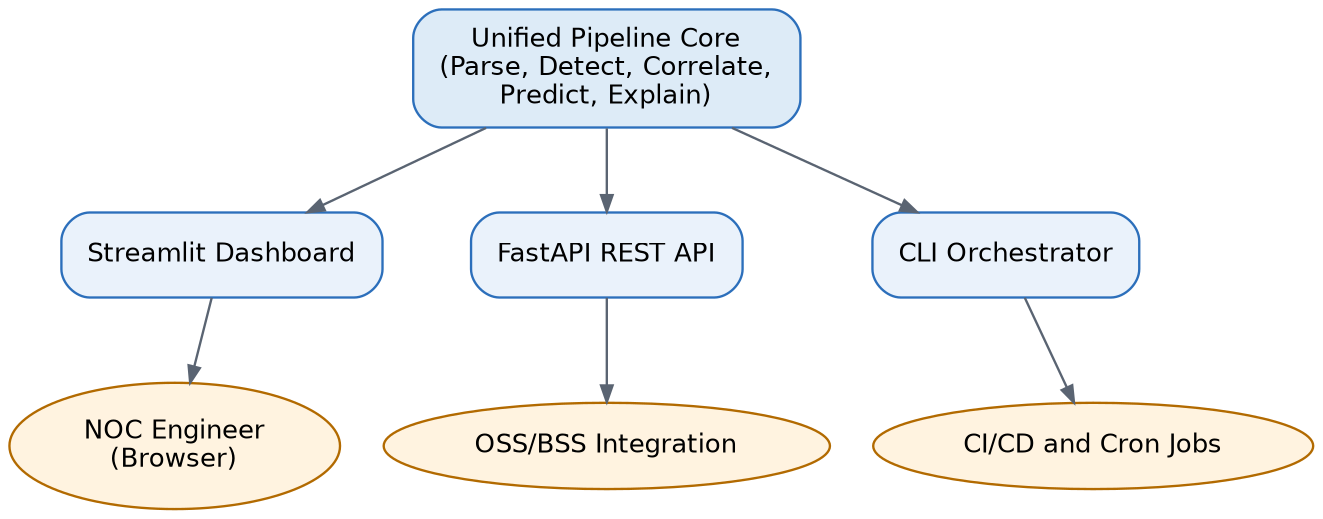
\includegraphics[width=0.85\textwidth]{figures/fig_5_10.png}
    \caption{Three Access Interfaces --- Three access interfaces (Dashboard, REST API, CLI) built on a shared pipeline core.}
    \label{fig:5_10}
\end{figure}

\begin{figure}[htbp]
    \centering
    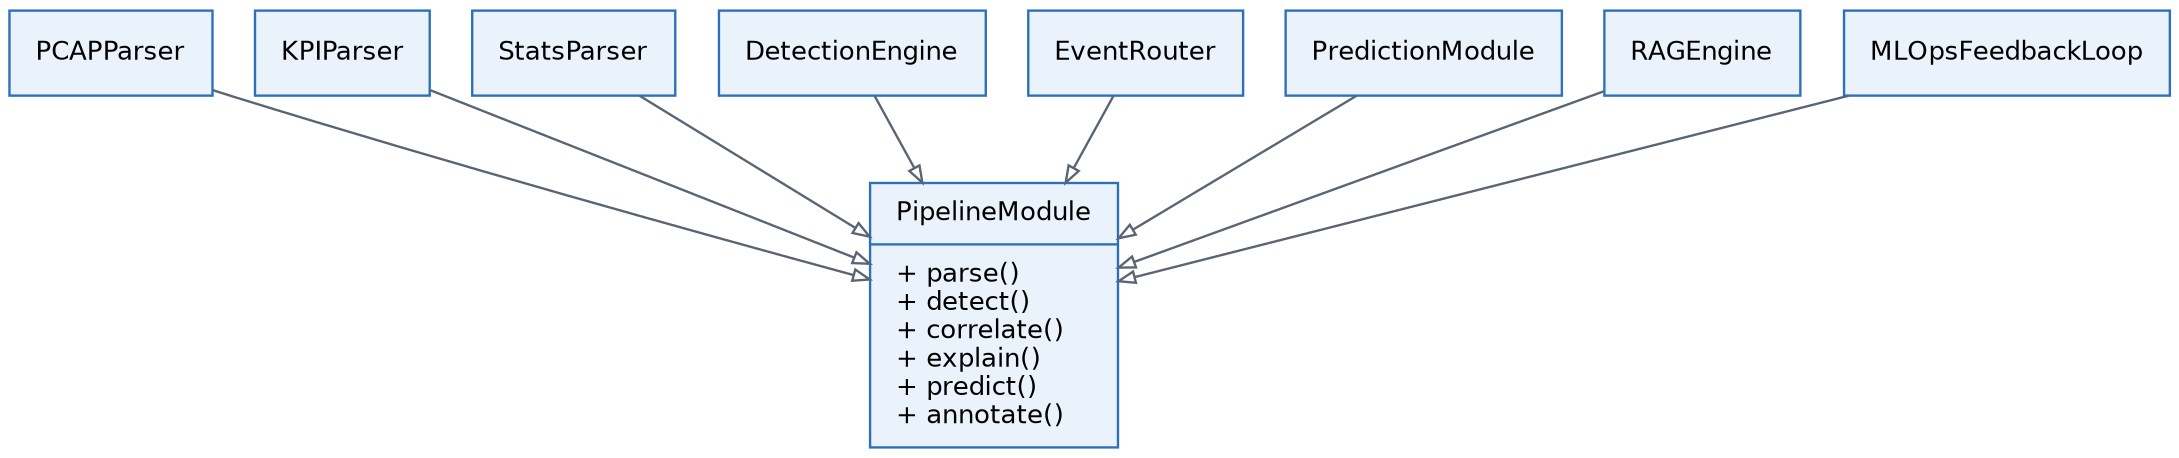
\includegraphics[width=0.85\textwidth]{figures/fig_5_11.png}
    \caption{Common Module Interface (Separation of Concerns) --- Common module interface enabling independent testing and future substitution of any pipeline component.}
    \label{fig:5_11}
\end{figure}

% ---------------- Chapter 6 ----------------
\begin{figure}[htbp]
    \centering
    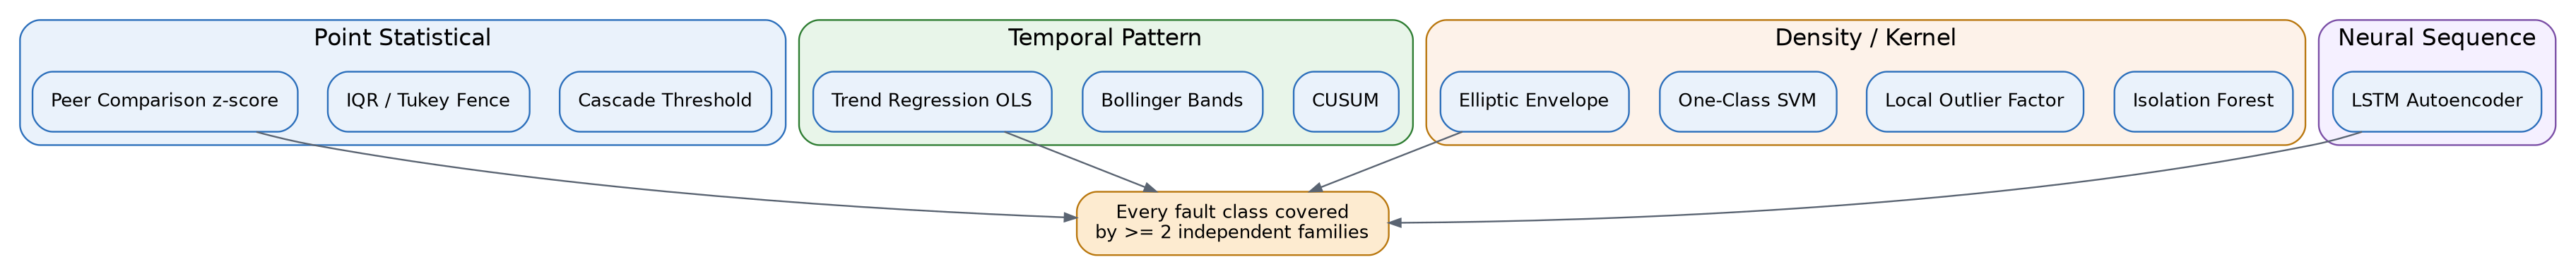
\includegraphics[width=0.85\textwidth]{figures/fig_6_1.png}
    \caption{Detector Family Taxonomy (Ensemble Coverage Principle) --- The twelve detection algorithms partitioned into four orthogonal families, the theoretical basis for the ensemble's fault-class coverage.}
    \label{fig:6_1}
\end{figure}

% ---------------- Chapter 7 ----------------
\begin{figure}[htbp]
    \centering
    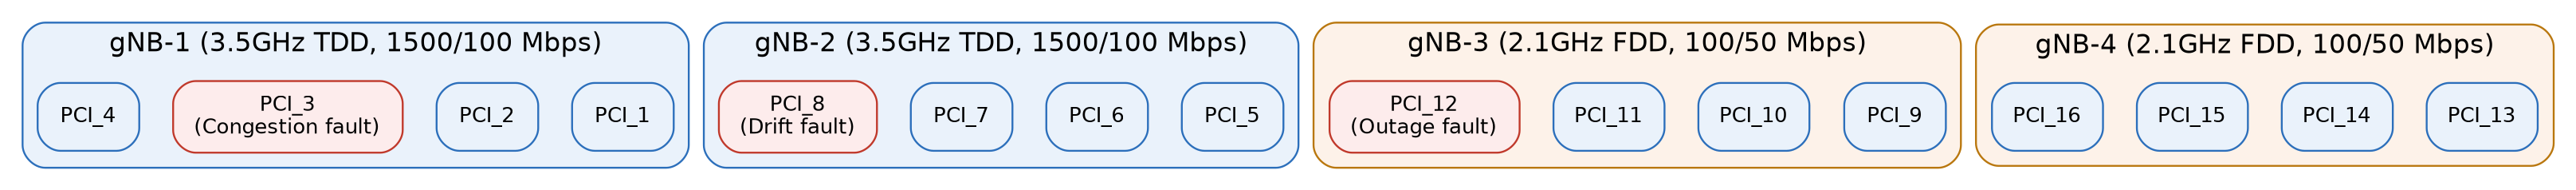
\includegraphics[width=0.85\textwidth]{figures/fig_7_1.png}
    \caption{Evaluation Network Topology --- Evaluation testbed topology: 4 gNBs / 16 cells / 64 UEs, with the three fault-injection cells highlighted.}
    \label{fig:7_1}
\end{figure}

\begin{figure}[htbp]
    \centering
    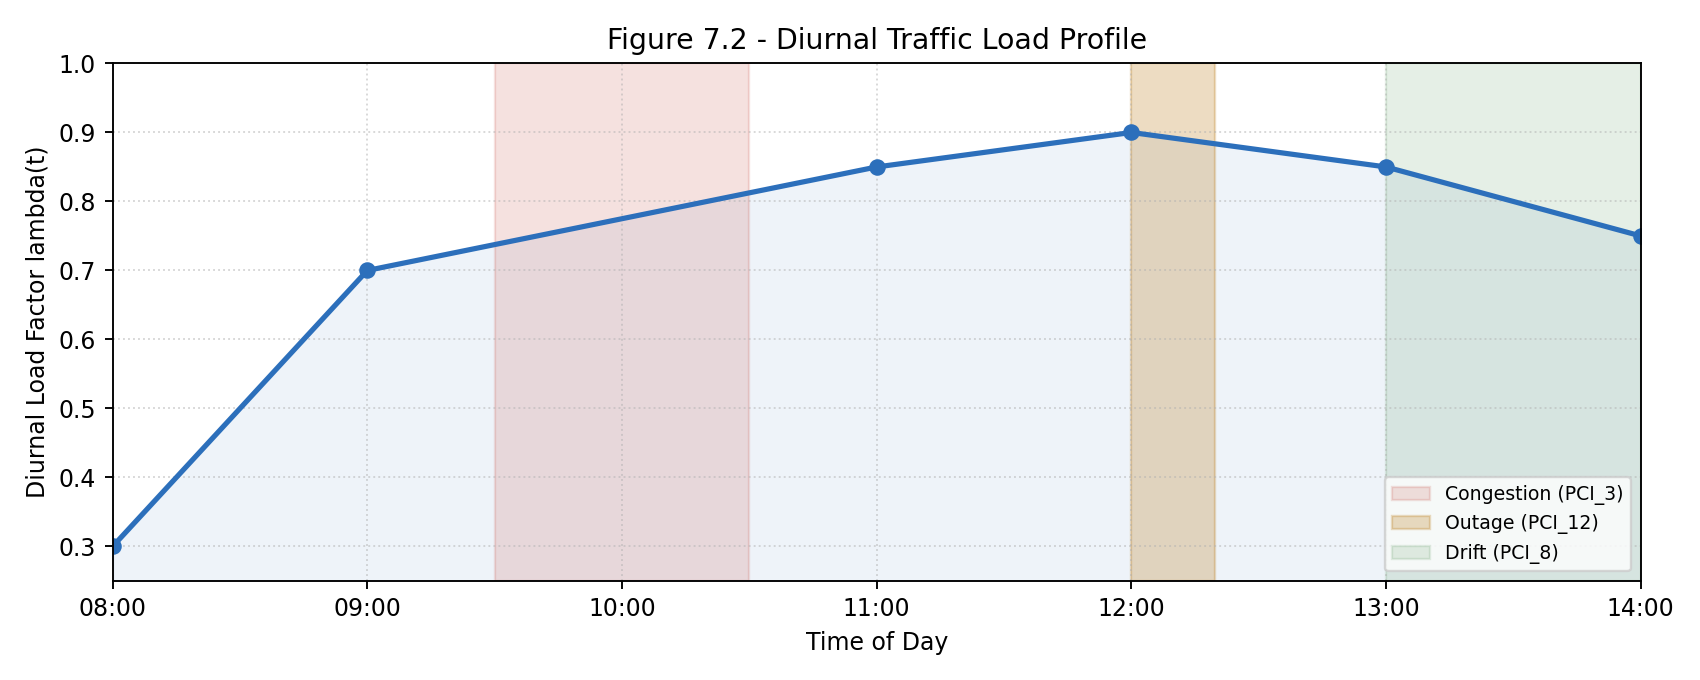
\includegraphics[width=0.85\textwidth]{figures/fig_7_2.png}
    \caption{Diurnal Traffic Load Profile --- Diurnal load factor over the 6-hour simulation window, with the three fault-injection windows marked.}
    \label{fig:7_2}
\end{figure}

\begin{figure}[htbp]
    \centering
    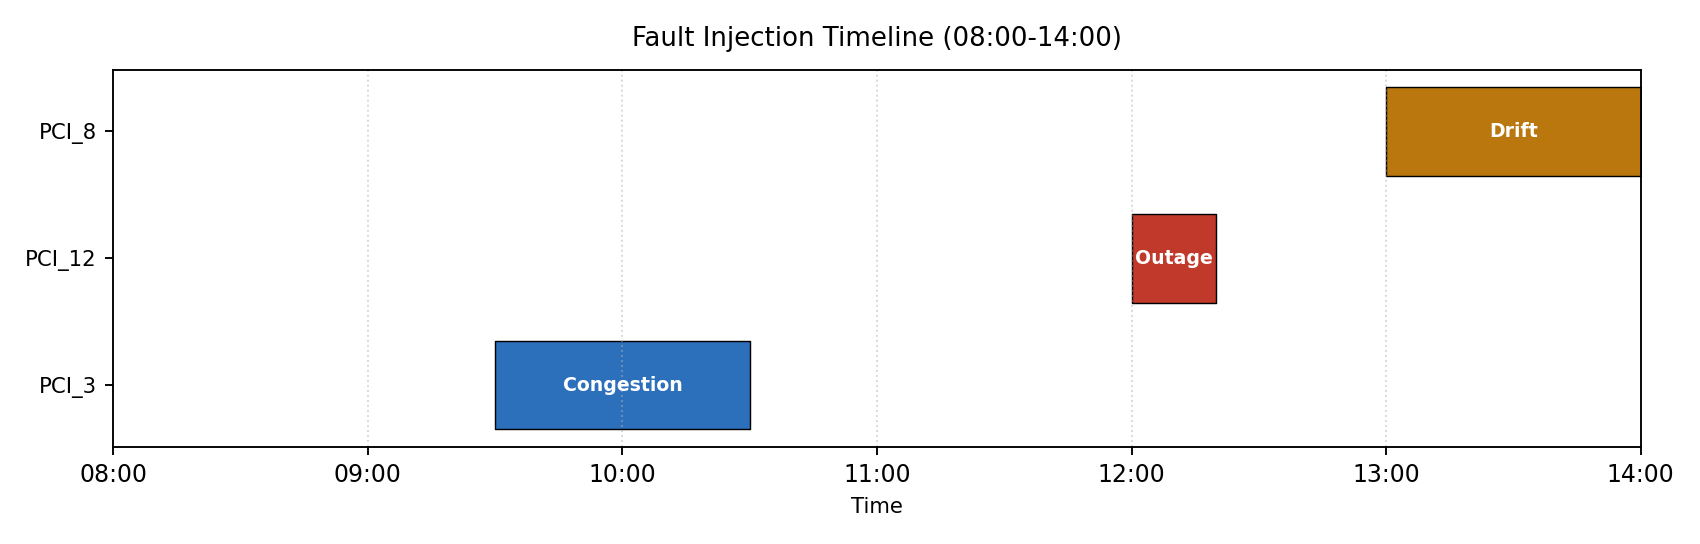
\includegraphics[width=0.85\textwidth]{figures/fig_7_3.png}
    \caption{Fault Injection Timeline --- Timeline of the three concurrent injected fault scenarios across the 6-hour evaluation window.}
    \label{fig:7_3}
\end{figure}

\begin{figure}[htbp]
    \centering
    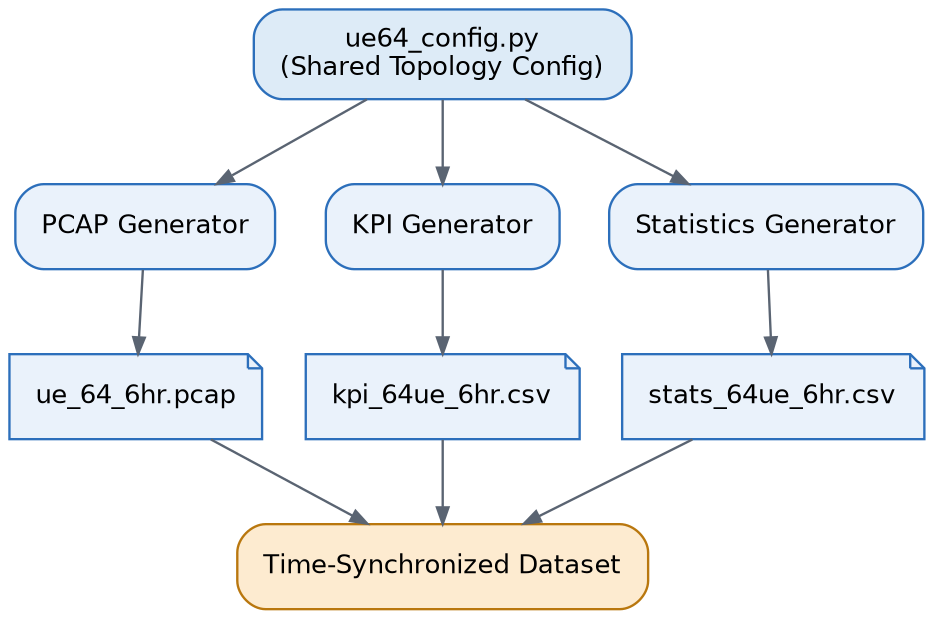
\includegraphics[width=0.85\textwidth]{figures/fig_7_4.png}
    \caption{Dataset Generation Pipeline --- Synthetic dataset generation pipeline: a single shared topology configuration produces three time-synchronized, cross-domain-consistent data files.}
    \label{fig:7_4}
\end{figure}

% ---------------- Chapter 8 ----------------
\begin{figure}[htbp]
    \centering
    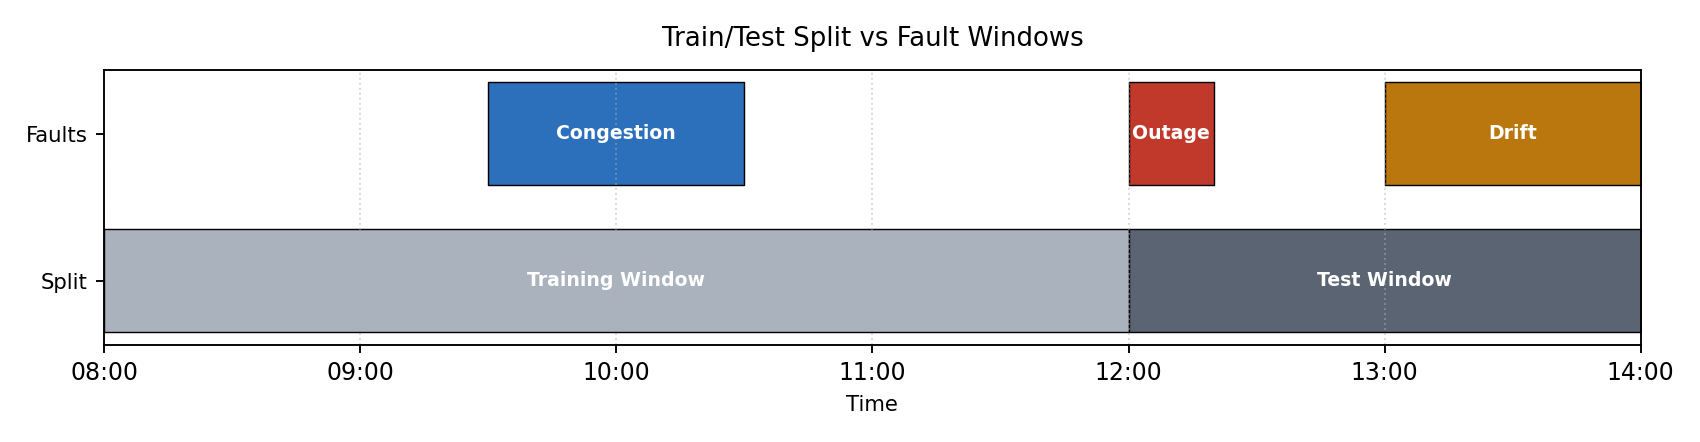
\includegraphics[width=0.85\textwidth]{figures/fig_8_1.png}
    \caption{Train/Test Temporal Split with Fault Overlay --- Temporal train/test split overlaid with the three fault windows, showing that the congestion fault straddles both windows while outage and drift fall entirely in the test window.}
    \label{fig:8_1}
\end{figure}

% ---------------- Chapter 9 ----------------
\begin{figure}[htbp]
    \centering
    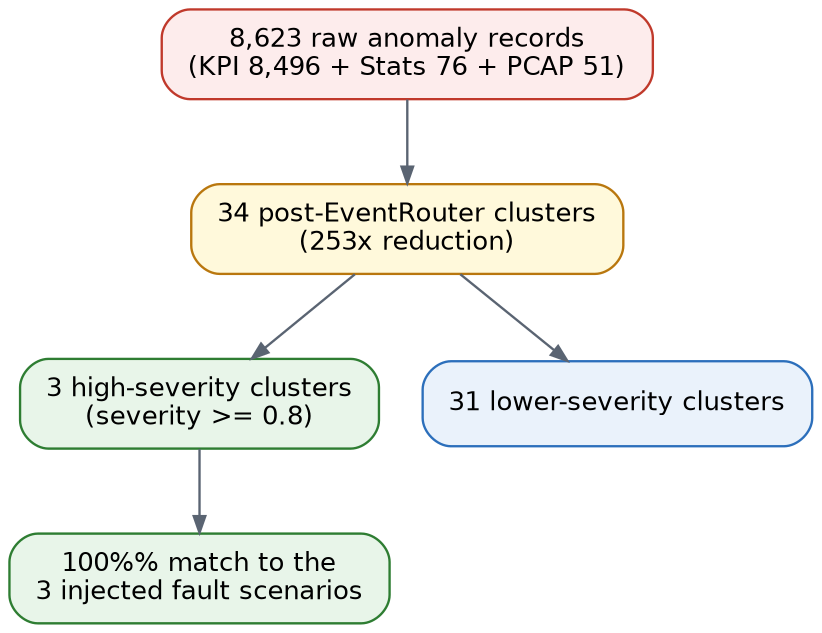
\includegraphics[width=0.85\textwidth]{figures/fig_9_1.png}
    \caption{EventRouter Alarm-Volume Reduction Funnel --- Alarm-volume reduction achieved by the EventRouter: 8,623 raw records collapse to 34 operator-visible clusters, with all three high-severity clusters correctly matching the injected faults.}
    \label{fig:9_1}
\end{figure}

\begin{figure}[htbp]
    \centering
    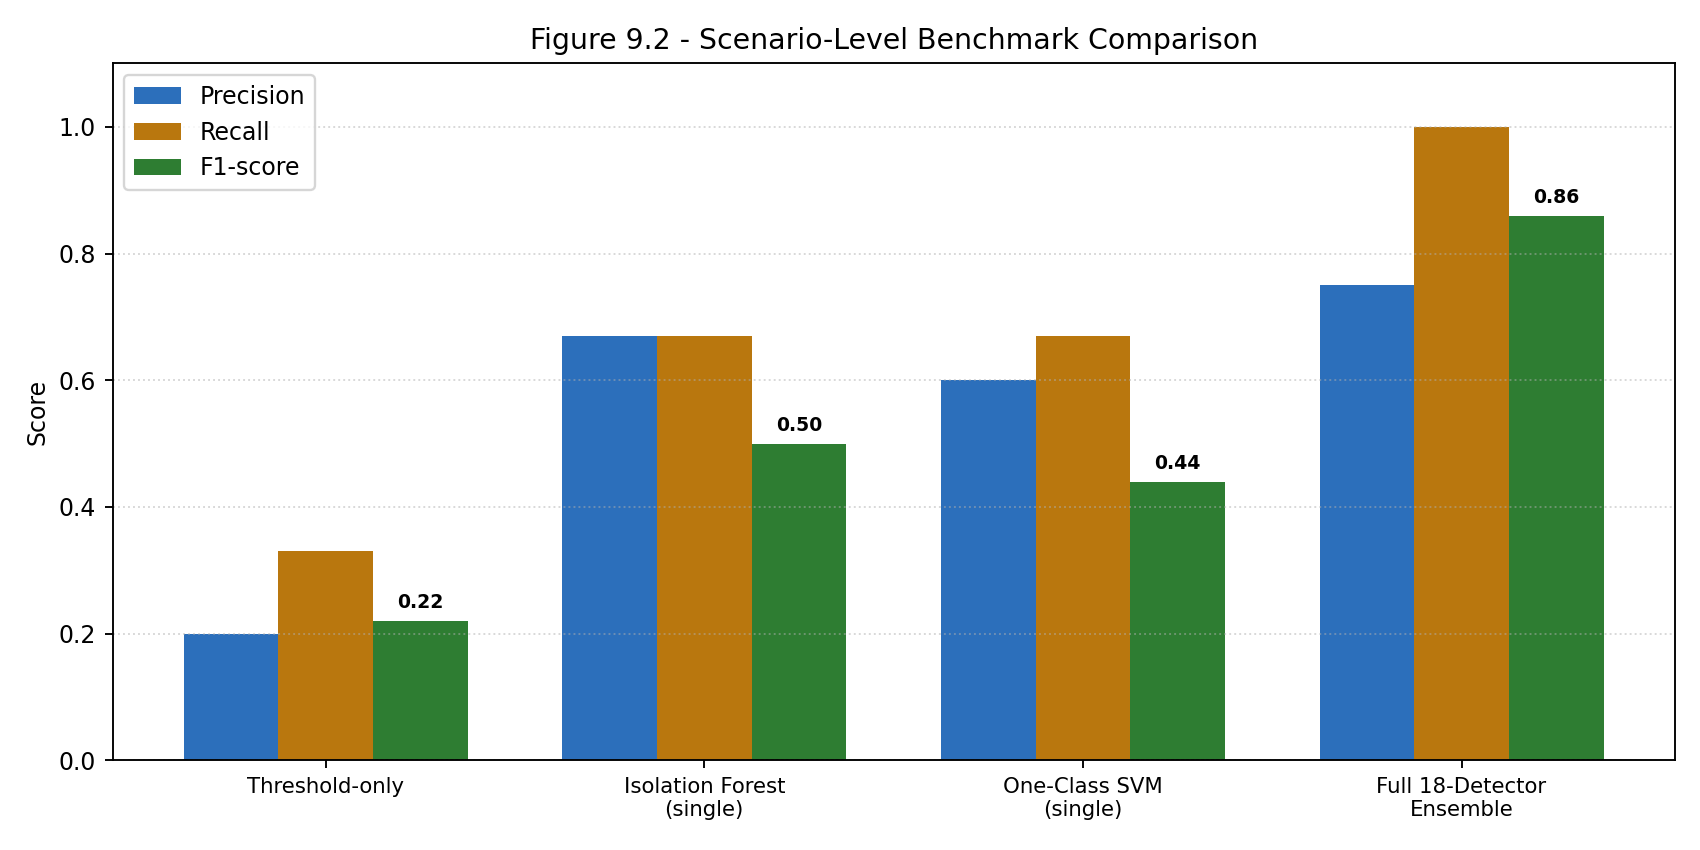
\includegraphics[width=0.85\textwidth]{figures/fig_9_2.png}
    \caption{Benchmark Comparison (Precision/Recall/F1) --- Scenario-level Precision, Recall, and F1 across the threshold-only baseline, two single-detector baselines, and the full 18-detector ensemble.}
    \label{fig:9_2}
\end{figure}

\begin{figure}[htbp]
    \centering
    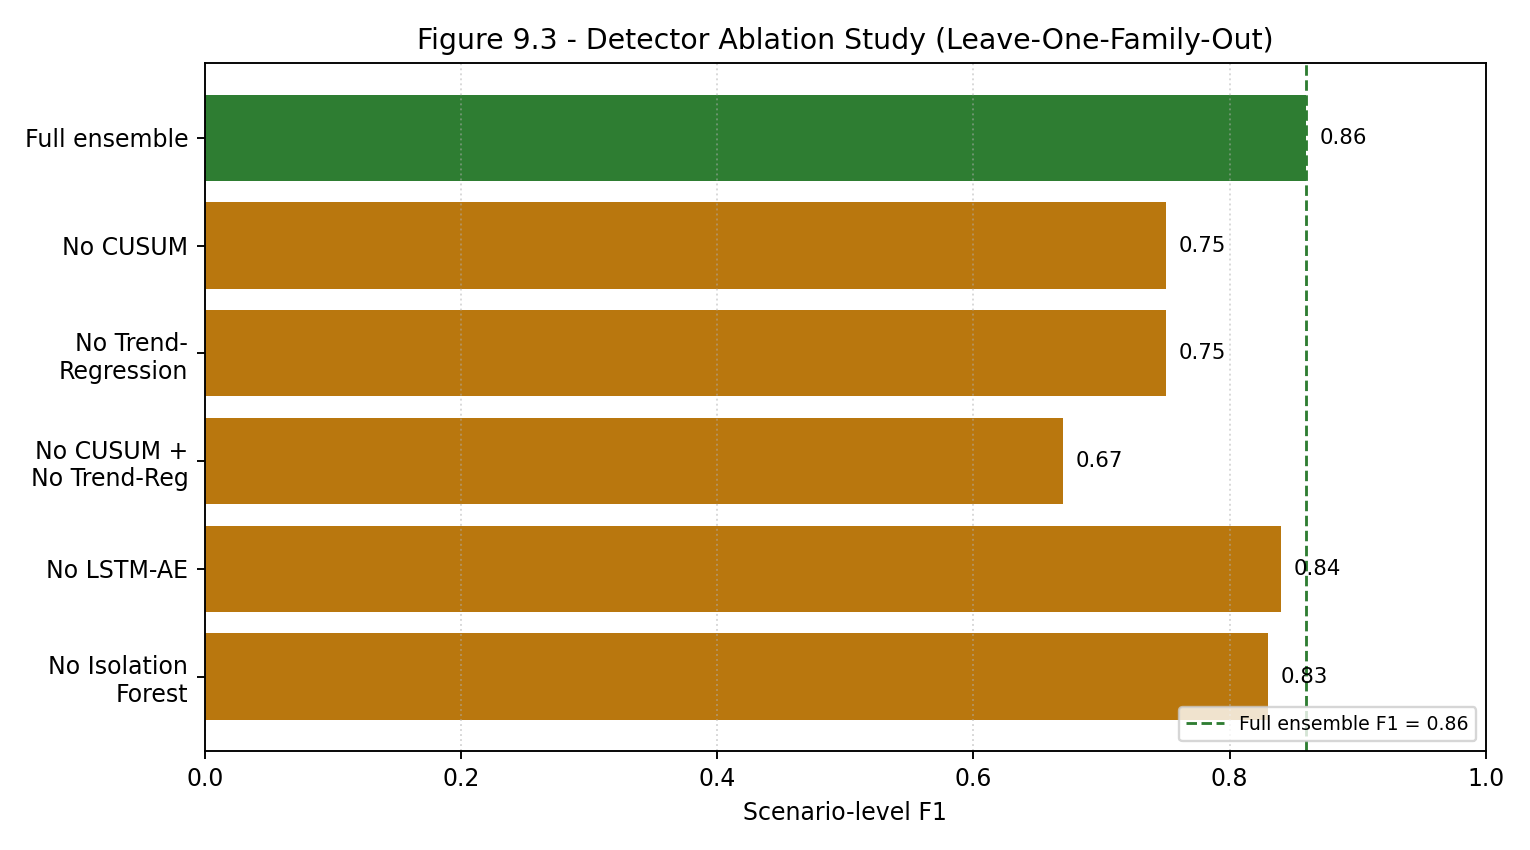
\includegraphics[width=0.85\textwidth]{figures/fig_9_3.png}
    \caption{Detector Ablation Study --- Leave-one-family-out ablation results, showing CUSUM and Trend-Regression as jointly necessary for slow-drift detection.}
    \label{fig:9_3}
\end{figure}

\begin{figure}[htbp]
    \centering
    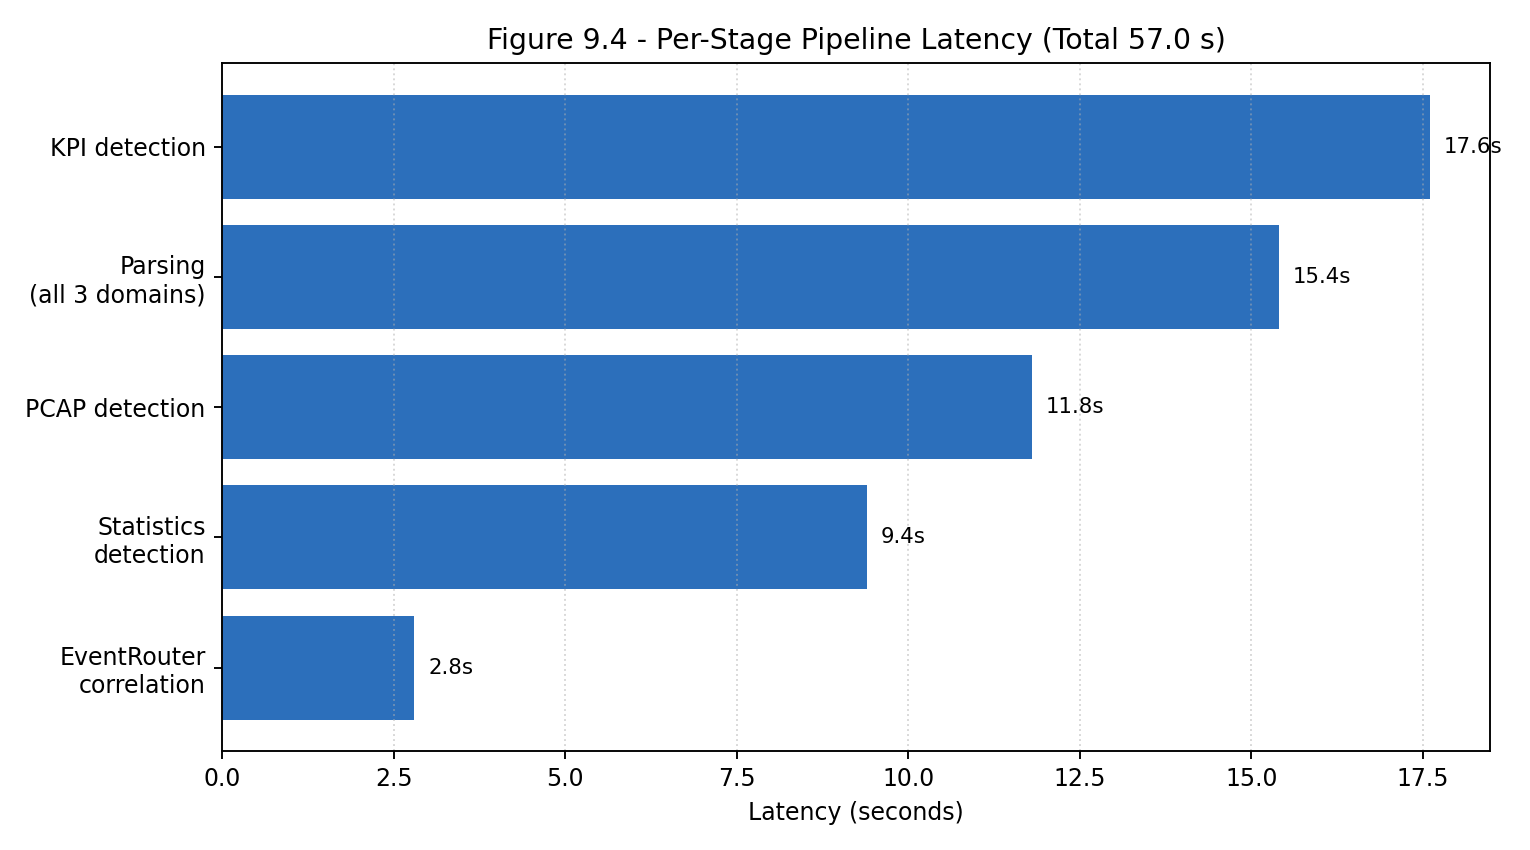
\includegraphics[width=0.85\textwidth]{figures/fig_9_4.png}
    \caption{Pipeline Latency Breakdown by Stage --- Per-stage latency breakdown of the 57-second end-to-end pipeline on the 64-UE dataset.}
    \label{fig:9_4}
\end{figure}

\begin{figure}[htbp]
    \centering
    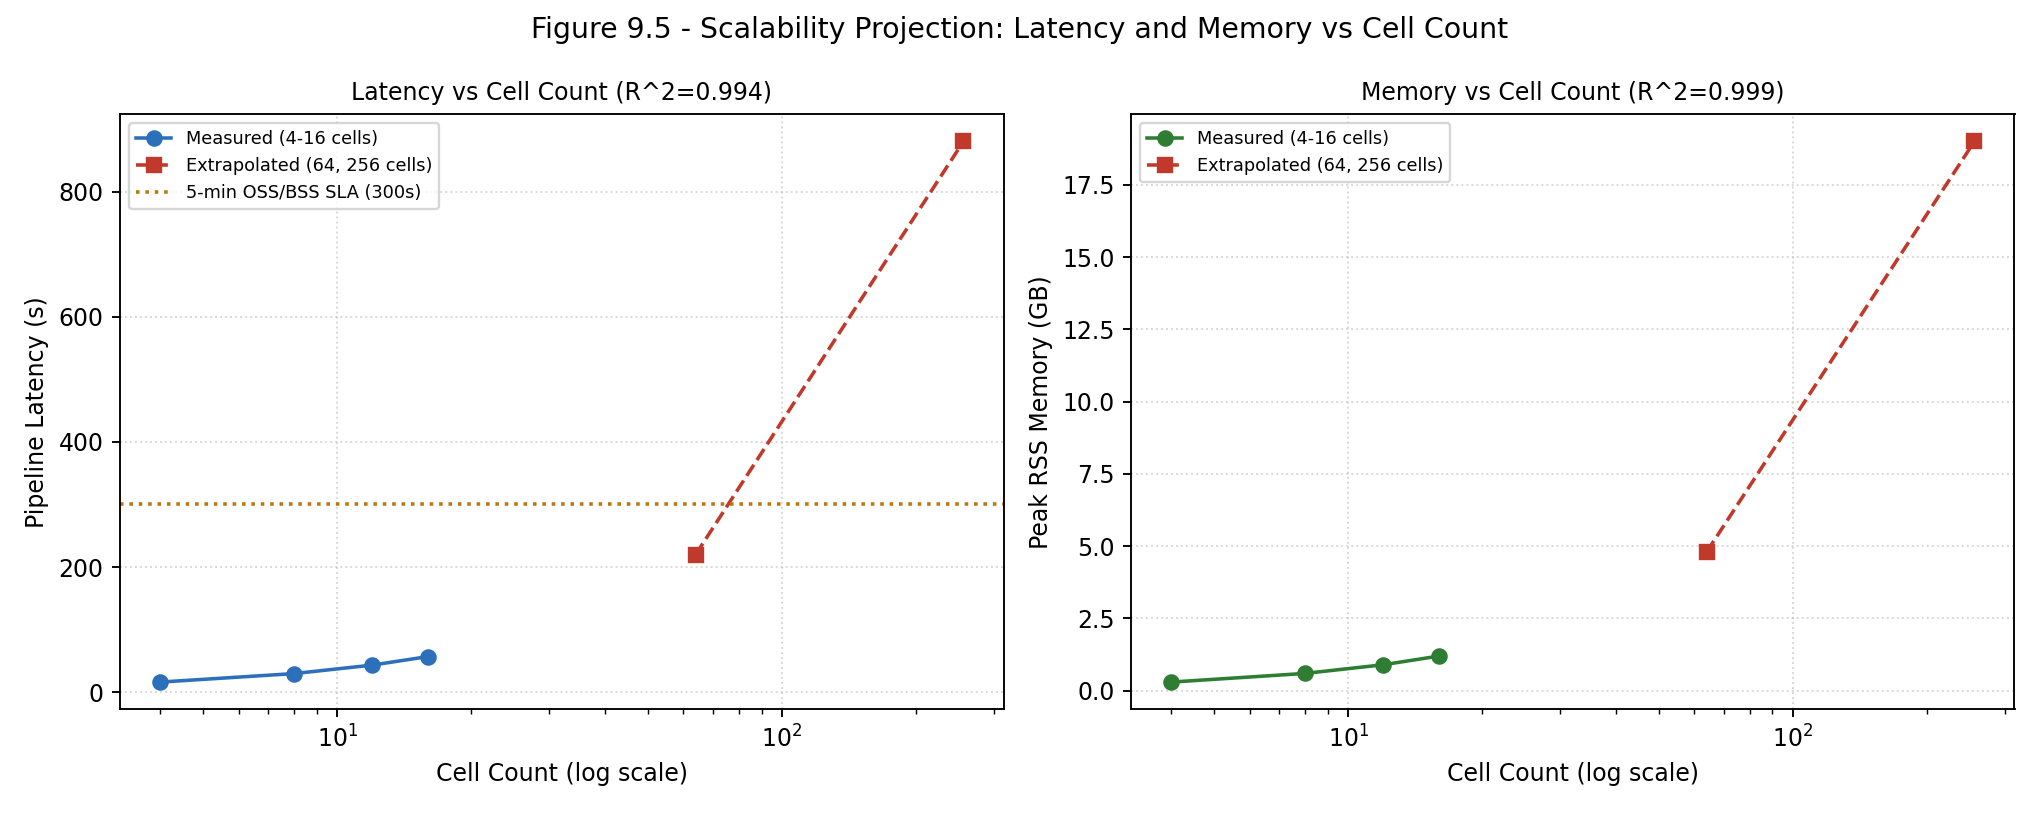
\includegraphics[width=0.85\textwidth]{figures/fig_9_5.png}
    \caption{Scalability Projection (Latency \& Memory vs. Cell Count) --- Measured (4 to 16 cells) and extrapolated (64, 256 cells) pipeline latency and peak memory, with the 5-minute OSS/BSS batch-cycle threshold marked.}
    \label{fig:9_5}
\end{figure}

% ---------------- Chapter 10 ----------------
\begin{figure}[htbp]
    \centering
    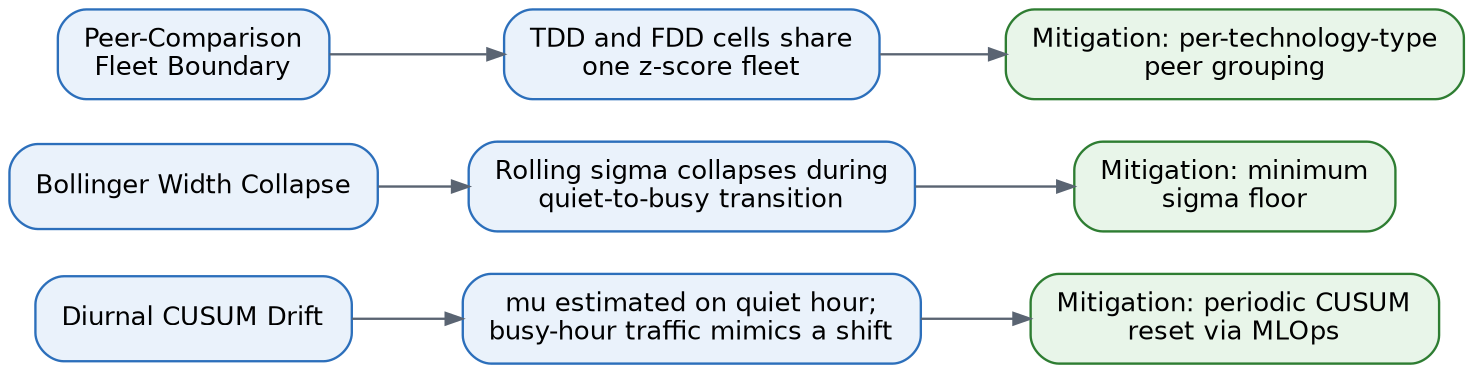
\includegraphics[width=0.85\textwidth]{figures/fig_10_1.png}
    \caption{False-Positive Root-Cause Map --- The three systematic sources of per-record false positives, their underlying mechanism, and the proposed mitigation for each.}
    \label{fig:10_1}
\end{figure}

% ---------------- Chapter 11 ----------------
\begin{figure}[htbp]
    \centering
    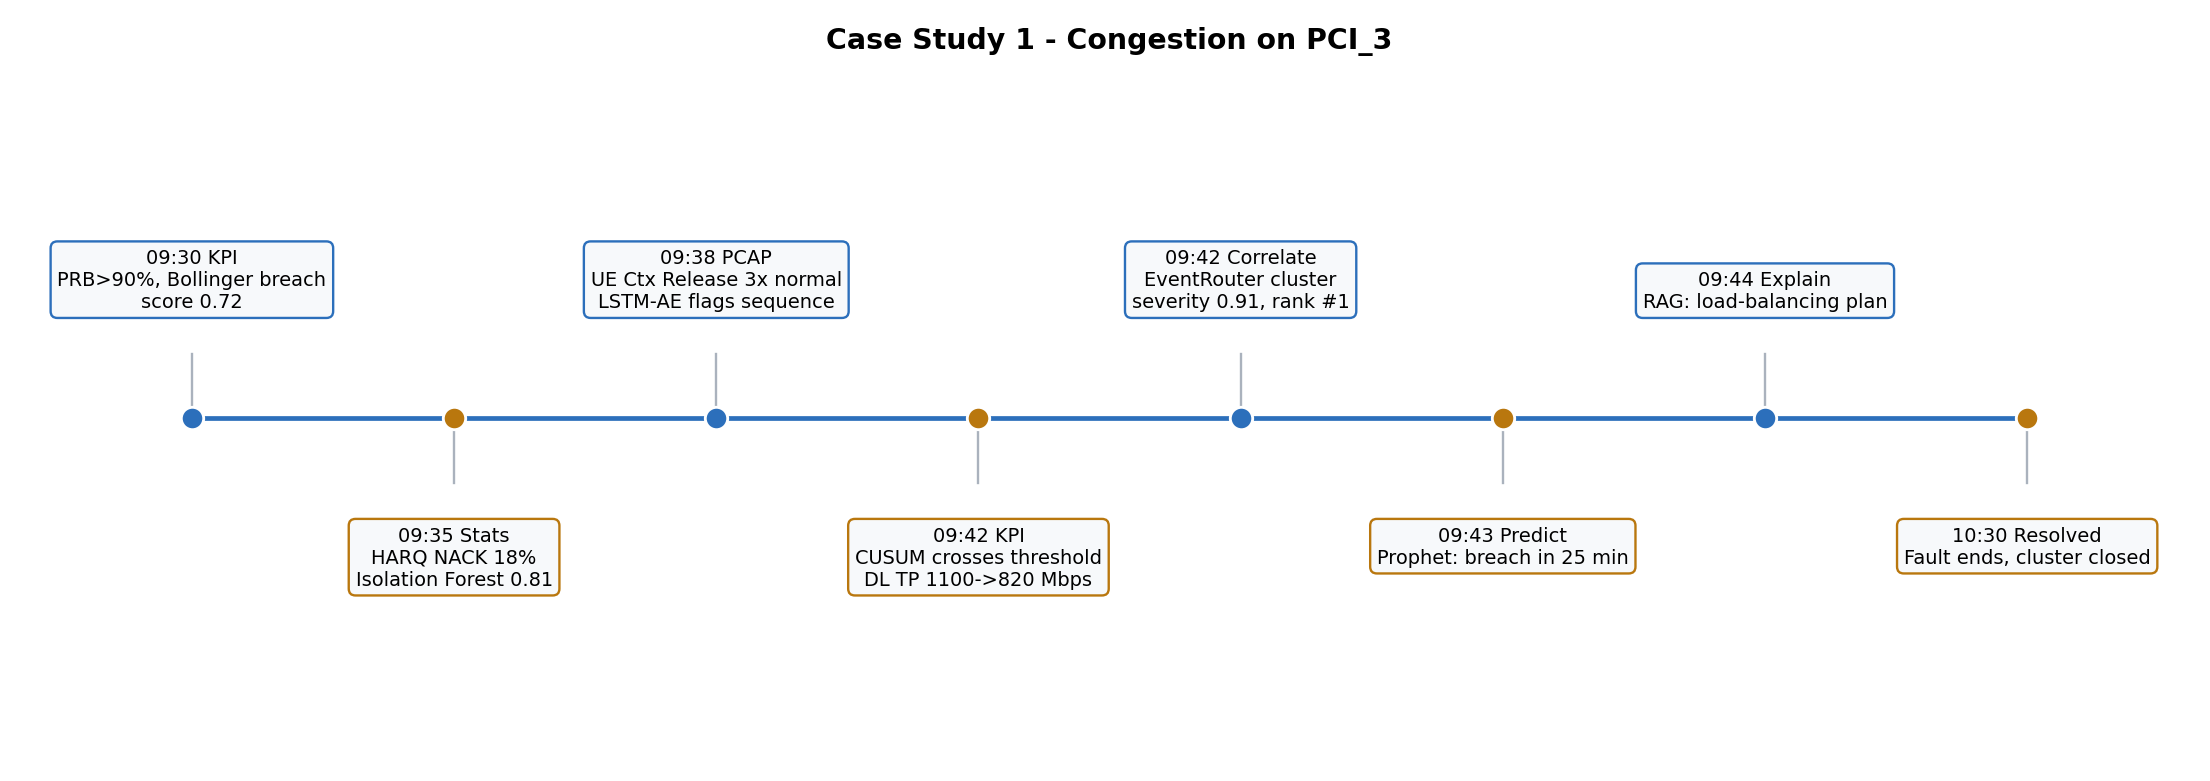
\includegraphics[width=0.85\textwidth]{figures/fig_11_1.png}
    \caption{Case Study 1 Timeline: Congestion on PCI_3 --- End-to-end pipeline trace for the PCI_3 congestion case study, from onset (09:30) to correlated detection (09:42) and explanation (09:44).}
    \label{fig:11_1}
\end{figure}

\begin{figure}[htbp]
    \centering
    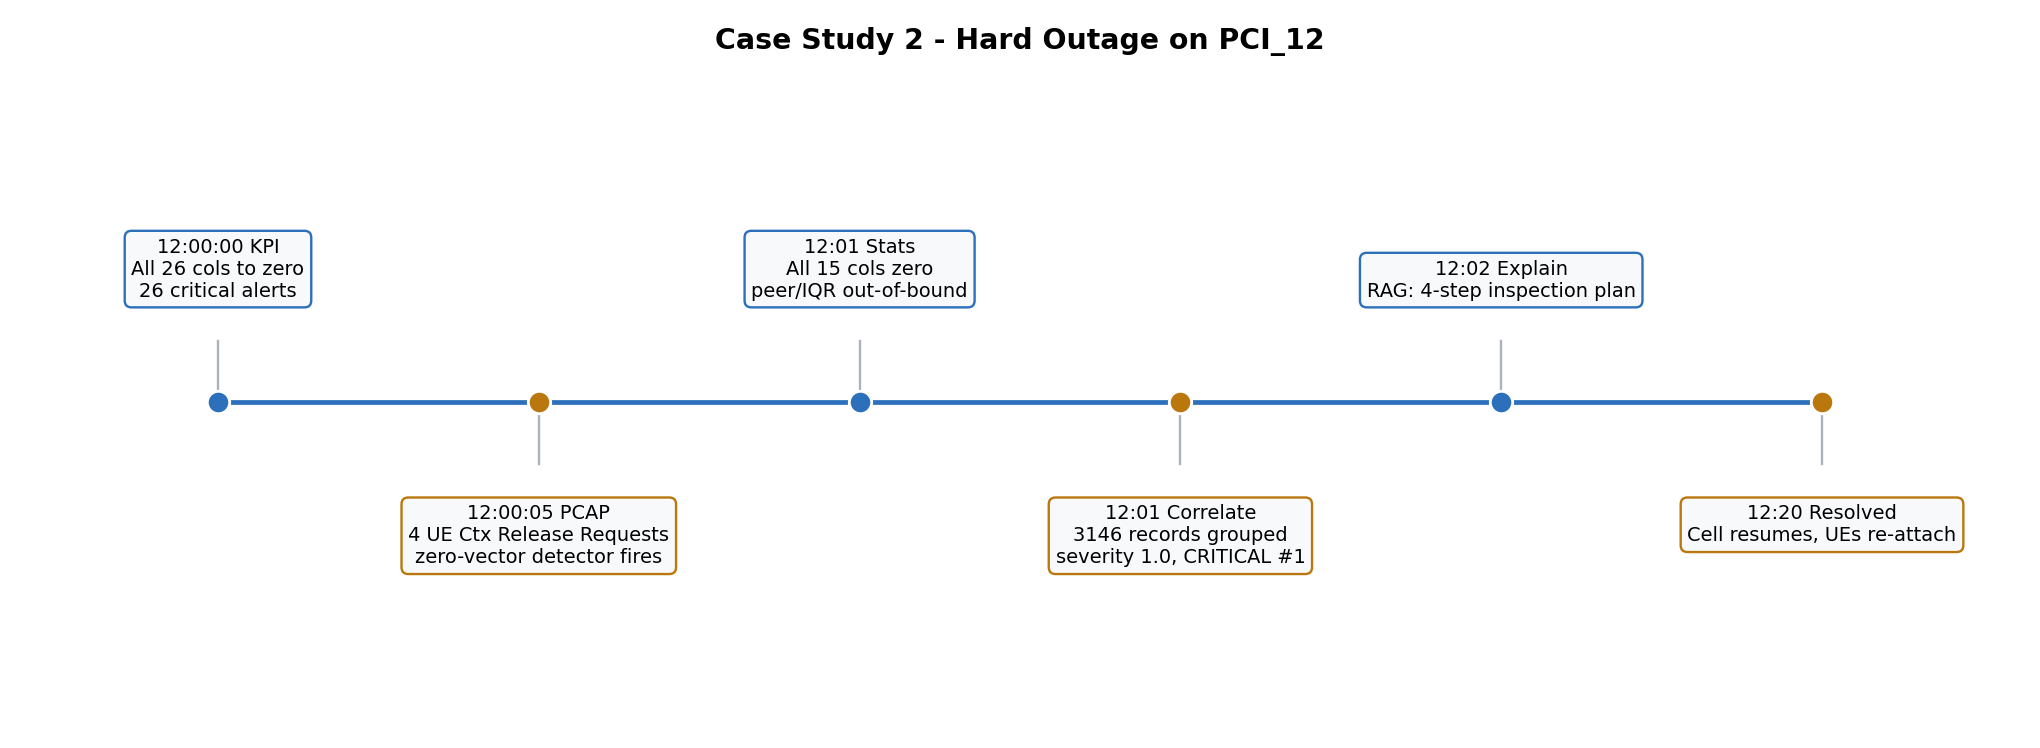
\includegraphics[width=0.85\textwidth]{figures/fig_11_2.png}
    \caption{Case Study 2 Timeline: Hard Outage on PCI_12 --- End-to-end pipeline trace for the PCI_12 hard outage, showing sub-minute detection and immediate severity-1.0 correlation.}
    \label{fig:11_2}
\end{figure}

\begin{figure}[htbp]
    \centering
    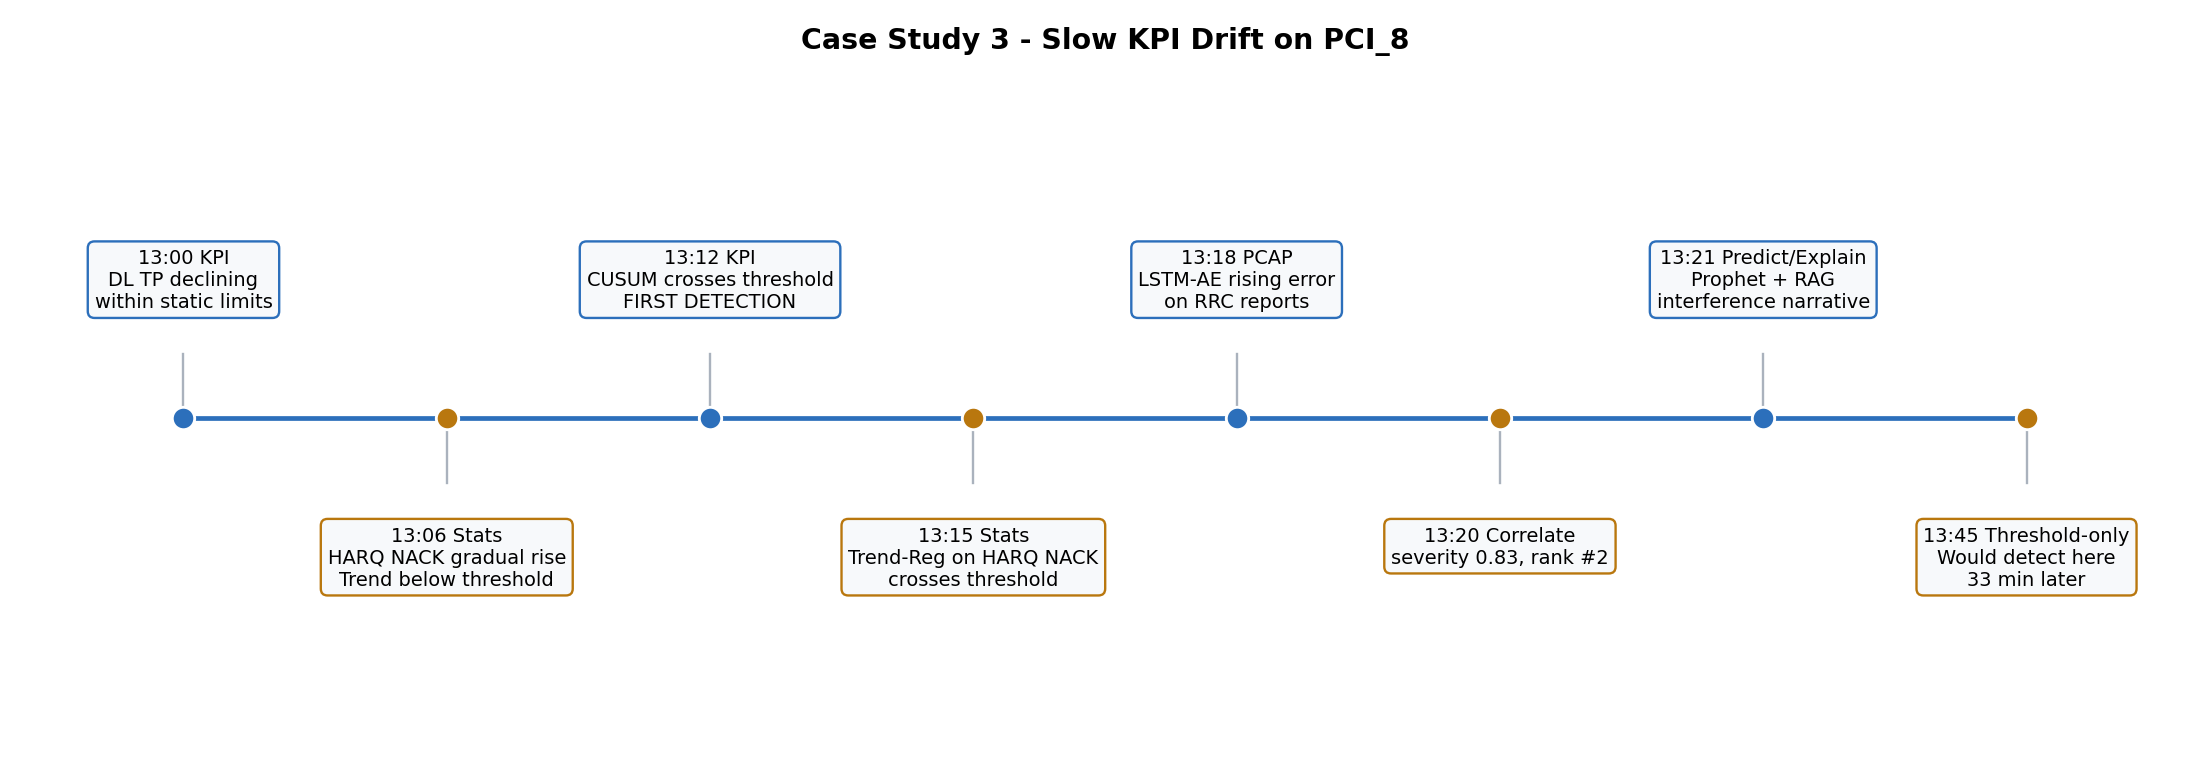
\includegraphics[width=0.85\textwidth]{figures/fig_11_3.png}
    \caption{Case Study 3 Timeline: Slow KPI Drift on PCI_8 --- End-to-end pipeline trace for the PCI_8 slow-drift case study, highlighting the 33-minute early-detection advantage of CUSUM over a threshold-only baseline.}
    \label{fig:11_3}
\end{figure}

% ---------------- Chapter 12 ----------------
\begin{figure}[htbp]
    \centering
    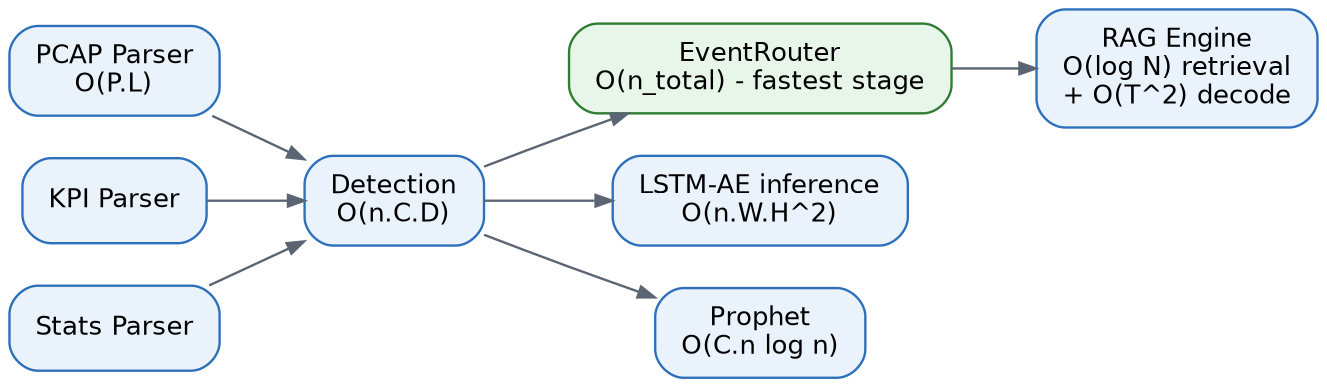
\includegraphics[width=0.85\textwidth]{figures/fig_12_1.png}
    \caption{Module-Level Complexity Overview --- Pipeline stages annotated with their asymptotic time complexity, showing the EventRouter as the fastest stage despite processing the largest input.}
    \label{fig:12_1}
\end{figure}

% ---------------- Chapter 14 ----------------
\begin{figure}[htbp]
    \centering
    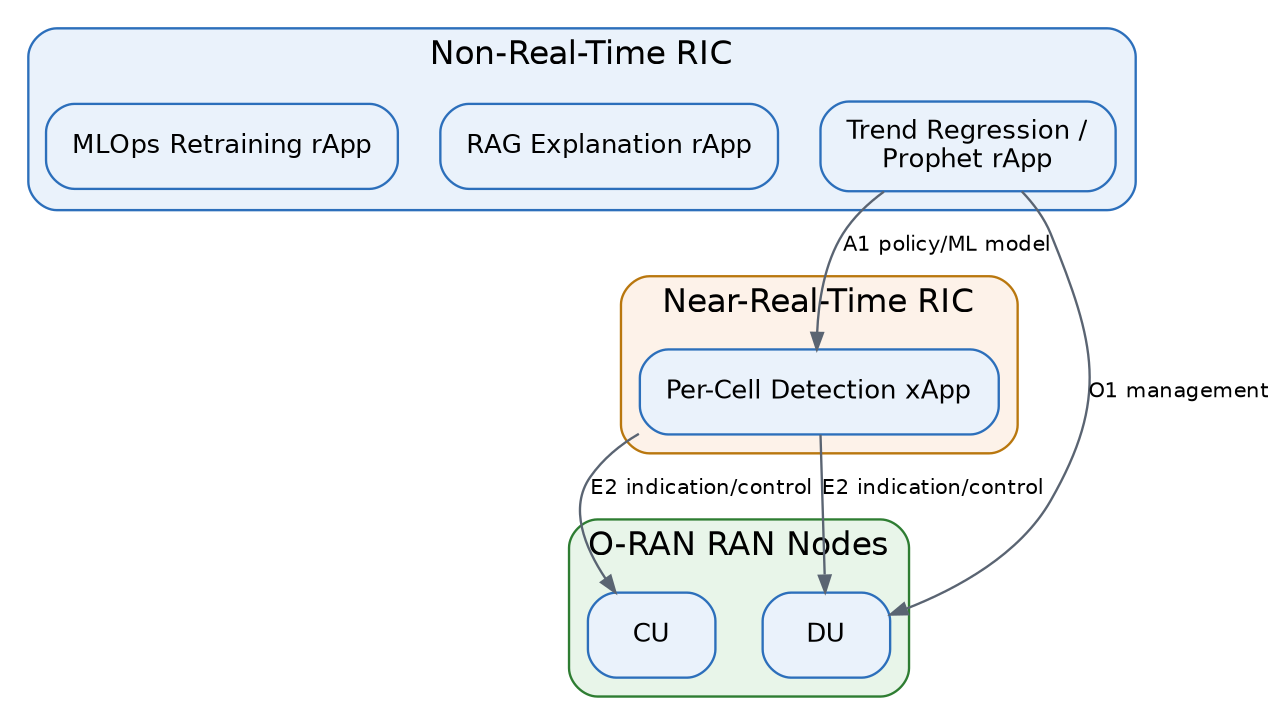
\includegraphics[width=0.85\textwidth]{figures/fig_14_1.png}
    \caption{O-RAN RIC Integration Architecture --- Mapping of the Unified Telecom Analyzer's pipeline modules onto the O-RAN Non-RT RIC (rApps) and Near-RT RIC (xApp) via the A1, O1, and E2 interfaces.}
    \label{fig:14_1}
\end{figure}

\begin{figure}[htbp]
    \centering
    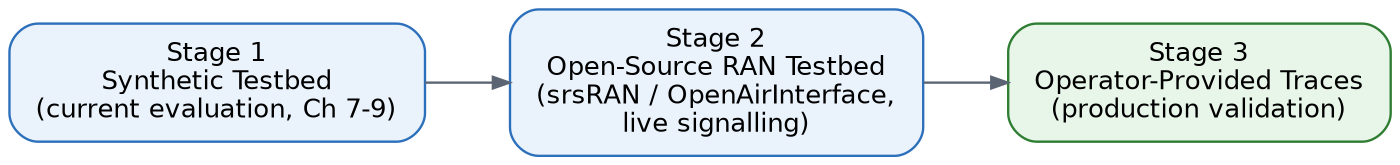
\includegraphics[width=0.85\textwidth]{figures/fig_14_2.png}
    \caption{Staged Production Validation Roadmap --- The staged validation path from the current synthetic evaluation to production deployment on operator traces.}
    \label{fig:14_2}
\end{figure}

\begin{figure}[htbp]
    \centering
    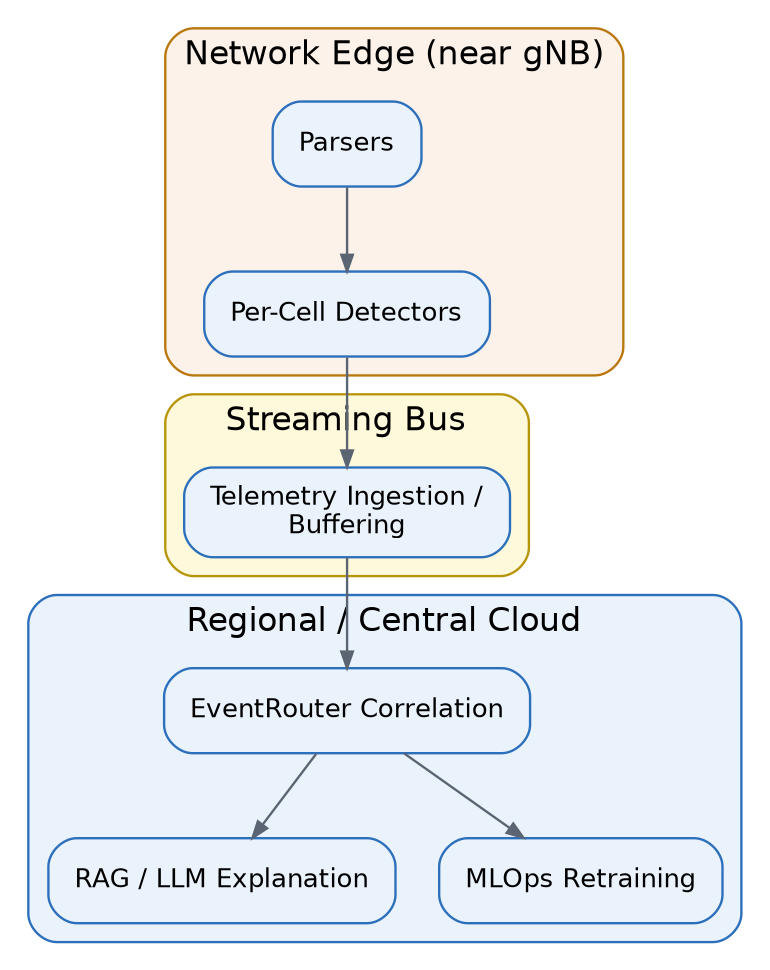
\includegraphics[width=0.85\textwidth]{figures/fig_14_3.png}
    \caption{Cloud-Native Deployment with Edge/Central Split --- Cloud-native deployment topology with latency-sensitive detection at the network edge and heavier RAG/LLM and retraining workloads in central/regional cloud.}
    \label{fig:14_3}
\end{figure}

% ---------------- Chapter 15 ----------------
\begin{figure}[htbp]
    \centering
    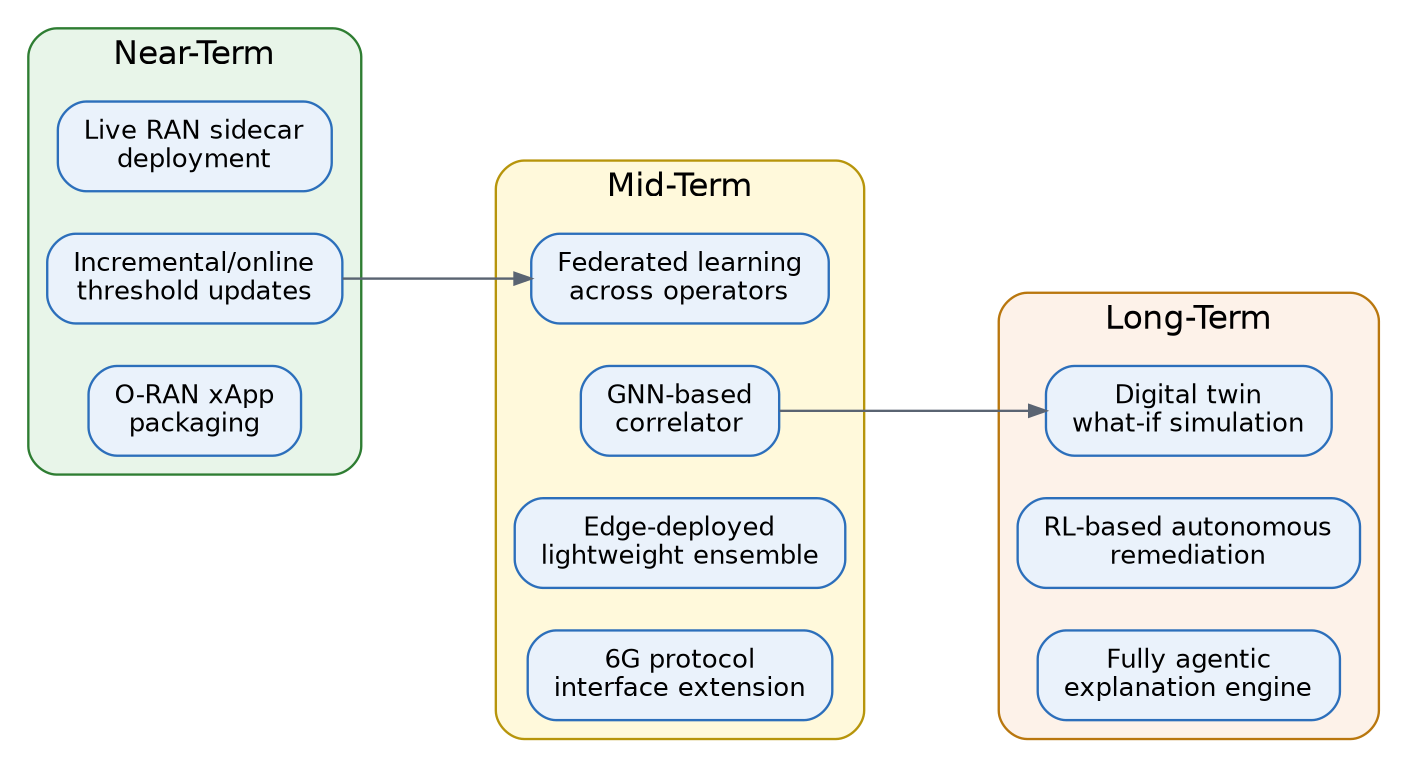
\includegraphics[width=0.85\textwidth]{figures/fig_15_1.png}
    \caption{Future Work Roadmap (Near-Term to Long-Term) --- The ten future work directions grouped by implementation horizon, from near-term engineering extensions to long-term autonomous-network research.}
    \label{fig:15_1}
\end{figure}

% ---------------- Chapter A ----------------
\begin{figure}[htbp]
    \centering
    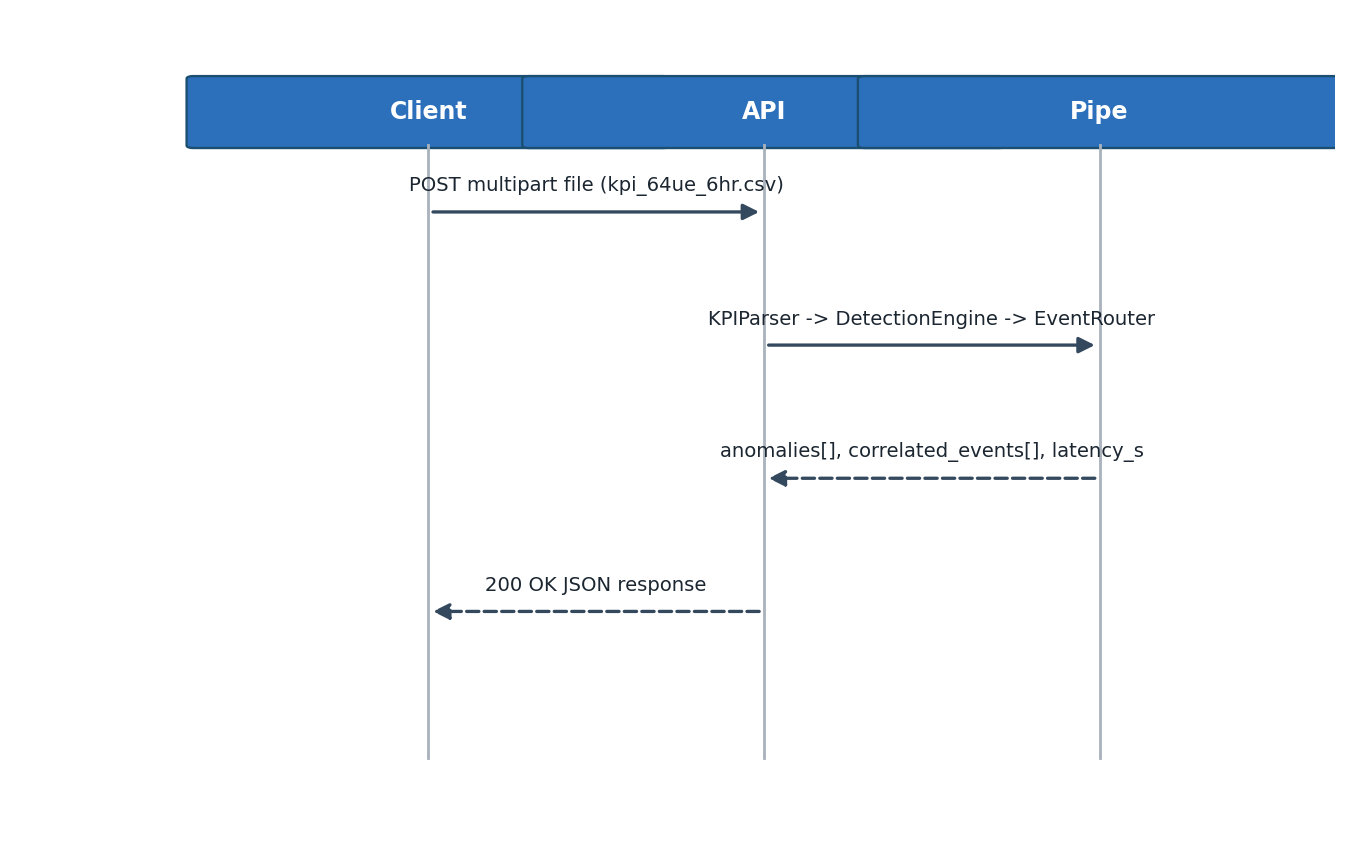
\includegraphics[width=0.85\textwidth]{figures/fig_A_1.png}
    \caption{Sample API Request/Response Flow --- Request/response sequence for the POST /analyze/kpi endpoint, from file upload through pipeline execution to JSON response.}
    \label{fig:A_1}
\end{figure}
  (place after \usepackage{graphicx})
% All images are in the figures/ subfolder - upload that folder to your Overleaf project root.
% ===================================================================

% ---------------- Chapter 1 ----------------
\begin{figure}[htbp]
    \centering
    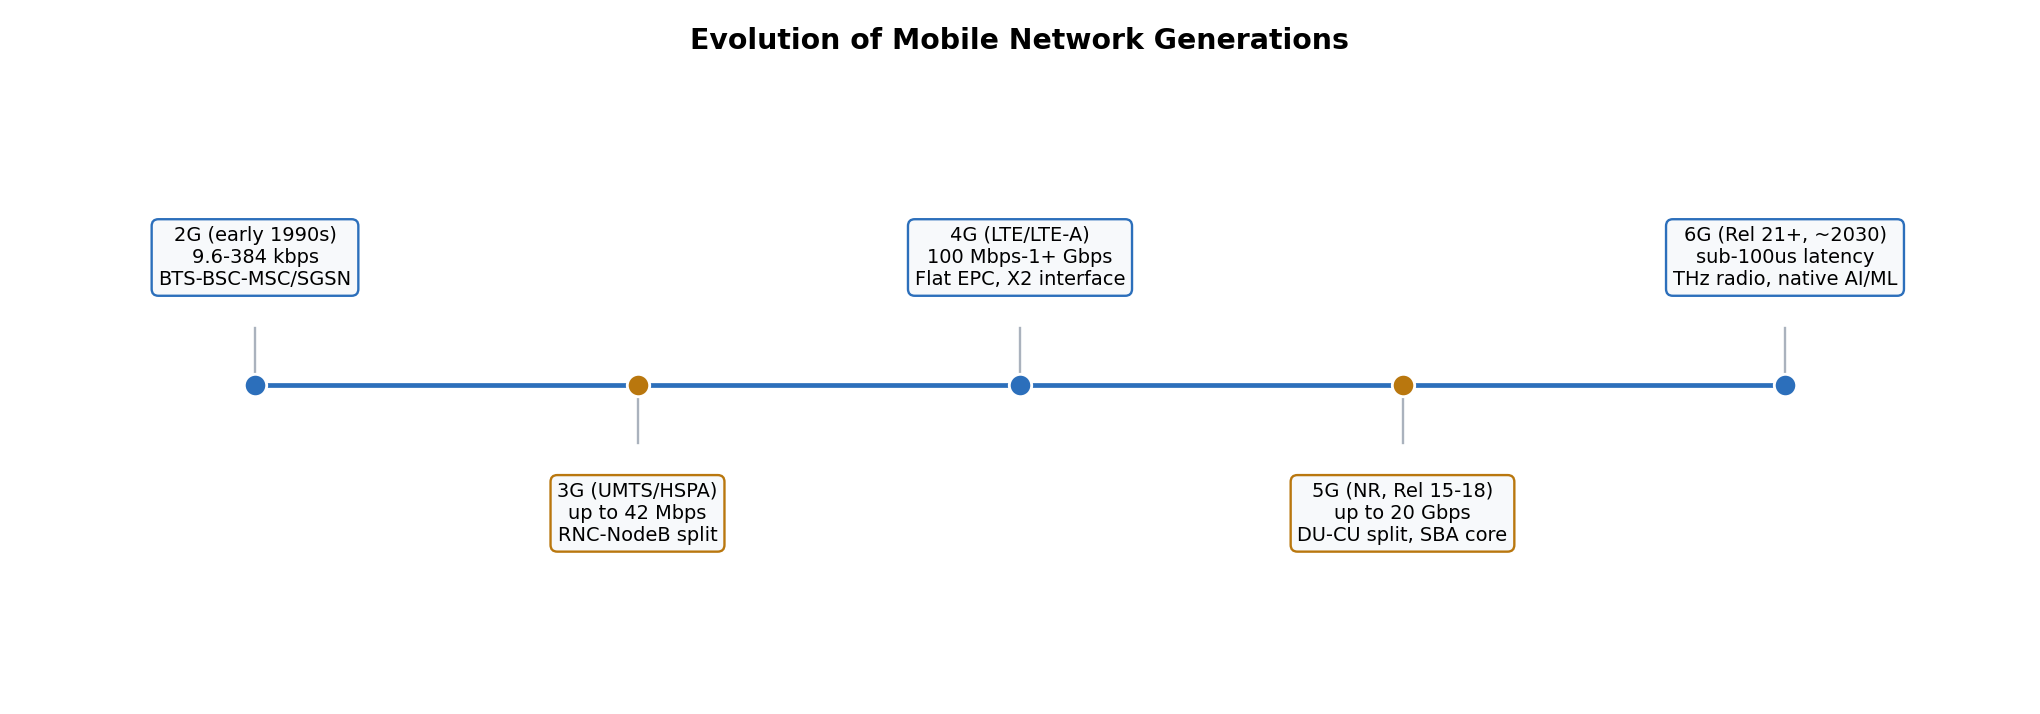
\includegraphics[width=0.85\textwidth]{figures/fig_1_1.png}
    \caption{Evolution of Mobile Network Generations --- Evolution of mobile network generations from 2G to the envisioned 6G, showing peak data rate and defining architectural change at each step.}
    \label{fig:1_1}
\end{figure}

\begin{figure}[htbp]
    \centering
    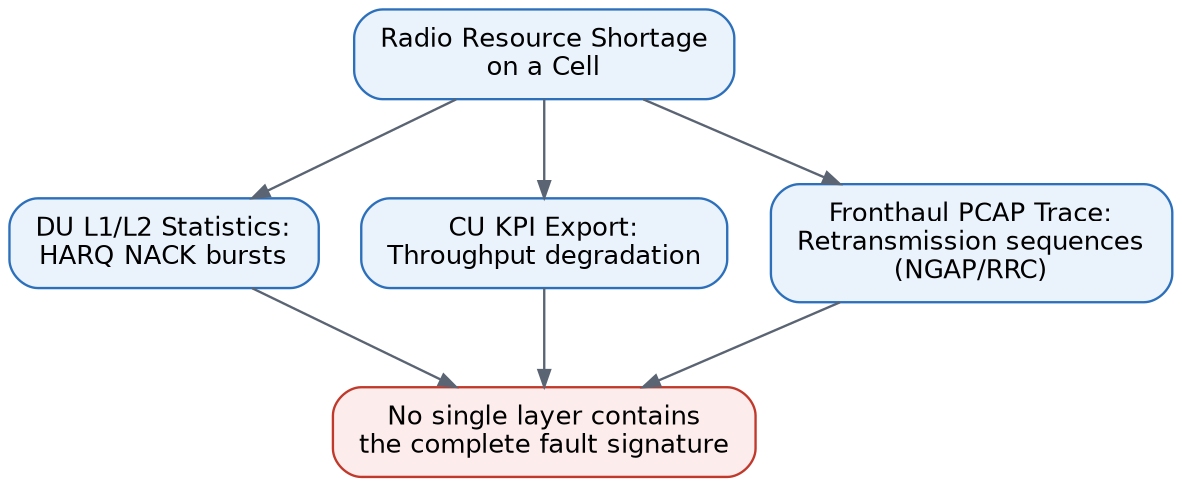
\includegraphics[width=0.85\textwidth]{figures/fig_1_2.png}
    \caption{Multi-Layer Fault Signature Propagation --- A single radio-resource fault propagates distinct, incomplete signatures into each of the three telemetry domains, motivating multi-modal detection.}
    \label{fig:1_2}
\end{figure}

\begin{figure}[htbp]
    \centering
    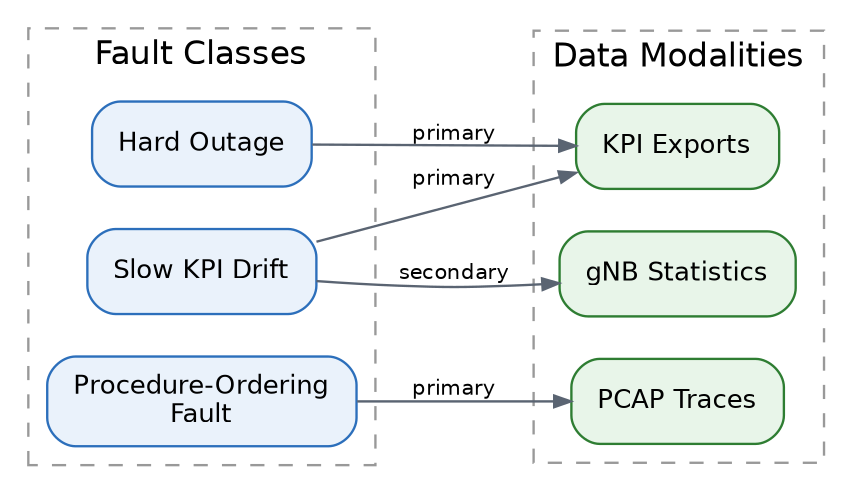
\includegraphics[width=0.85\textwidth]{figures/fig_1_3.png}
    \caption{Complementary Fault Coverage of the Three Modalities --- Mapping of the three targeted fault classes to their primary detecting modality, illustrating why no single data source covers the full fault taxonomy.}
    \label{fig:1_3}
\end{figure}

% ---------------- Chapter 2 ----------------
\begin{figure}[htbp]
    \centering
    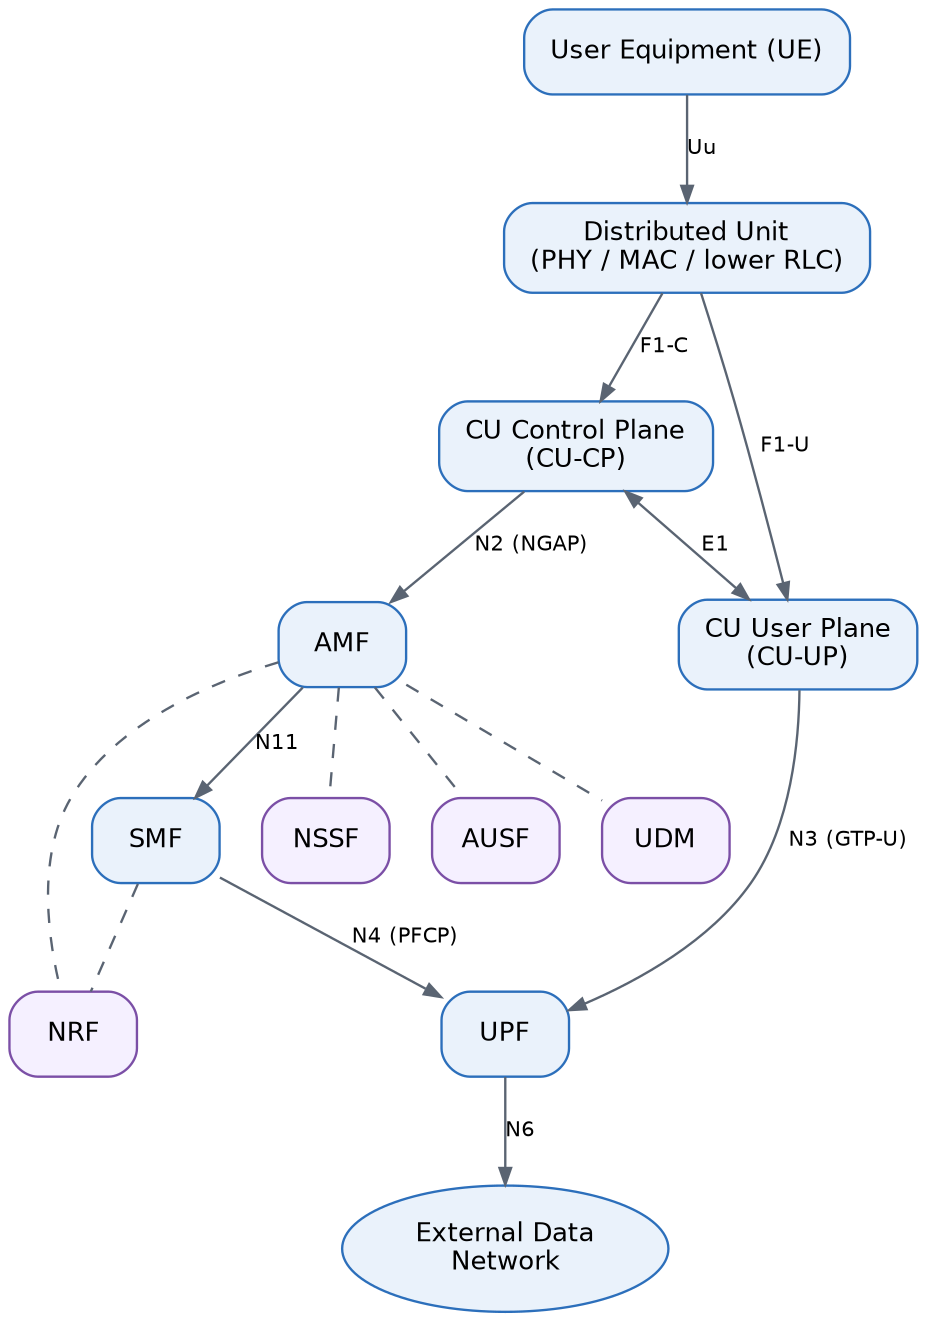
\includegraphics[width=0.85\textwidth]{figures/fig_2_1.png}
    \caption{5G Network Architecture (NG-RAN + 5GC) --- 5G system architecture showing the disaggregated NG-RAN (DU/CU-CP/CU-UP) and the Service-Based Architecture of the 5G Core.}
    \label{fig:2_1}
\end{figure}

\begin{figure}[htbp]
    \centering
    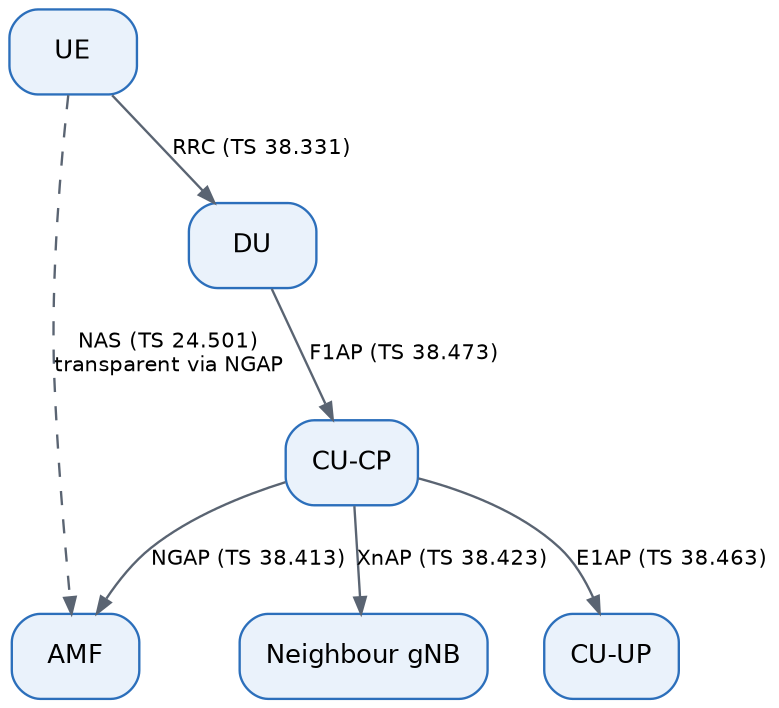
\includegraphics[width=0.85\textwidth]{figures/fig_2_2.png}
    \caption{Six Protocol Interfaces Mapped to Network Nodes --- The six 5G-NR protocol interfaces parsed by the PCAP Parser, mapped to their governing 3GPP specification and network-node endpoints.}
    \label{fig:2_2}
\end{figure}

% ---------------- Chapter 3 ----------------
\begin{figure}[htbp]
    \centering
    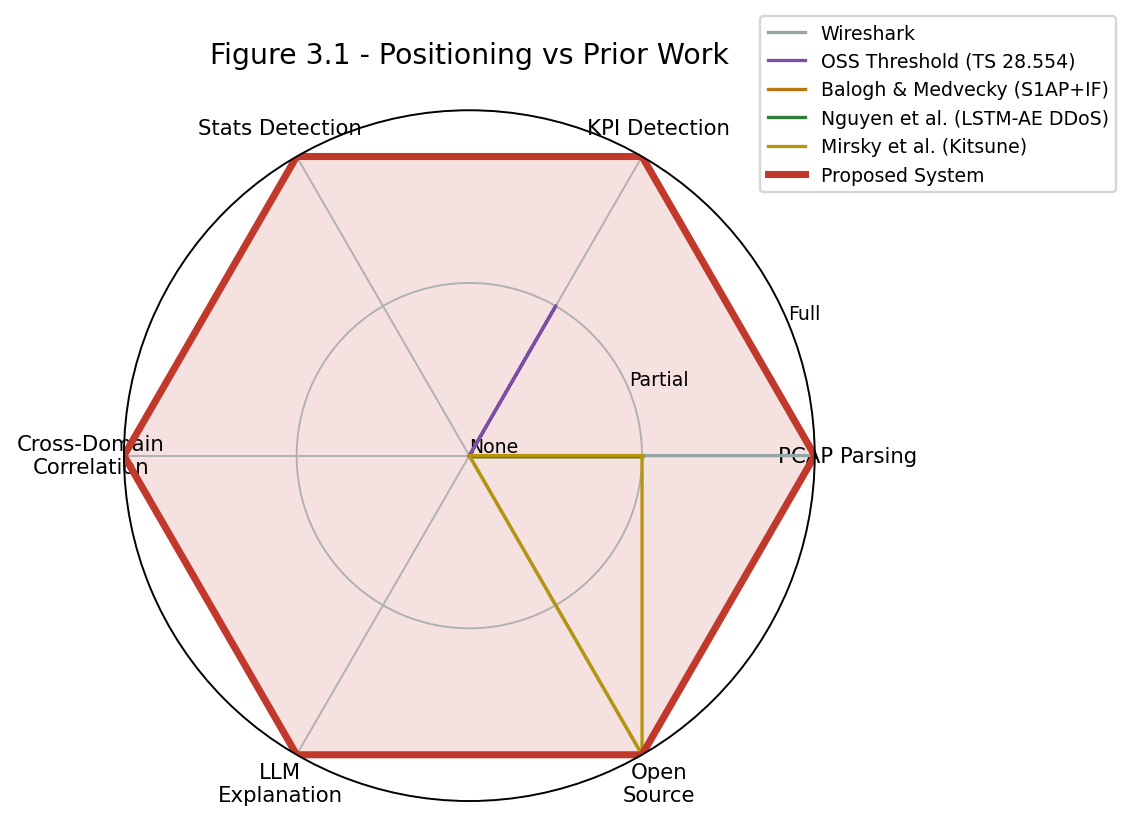
\includegraphics[width=0.85\textwidth]{figures/fig_3_1.png}
    \caption{Positioning Comparison vs. Prior Work --- Radar comparison of the proposed system against five representative prior systems across the five positioning axes of Table 3.1.}
    \label{fig:3_1}
\end{figure}

% ---------------- Chapter 4 ----------------
\begin{figure}[htbp]
    \centering
    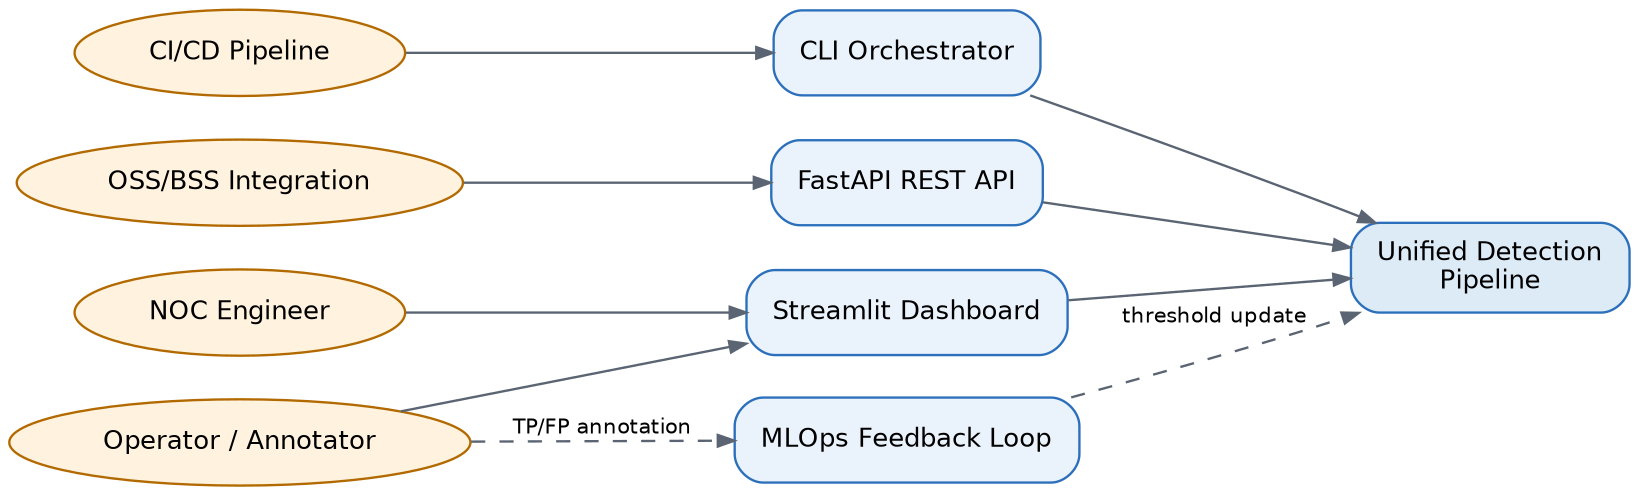
\includegraphics[width=0.85\textwidth]{figures/fig_4_1.png}
    \caption{Use Case Diagram --- Actors and access interfaces for the Unified Telecom Analyzer, tracing each functional requirement to its consuming role.}
    \label{fig:4_1}
\end{figure}

% ---------------- Chapter 5 ----------------
\begin{figure}[htbp]
    \centering
    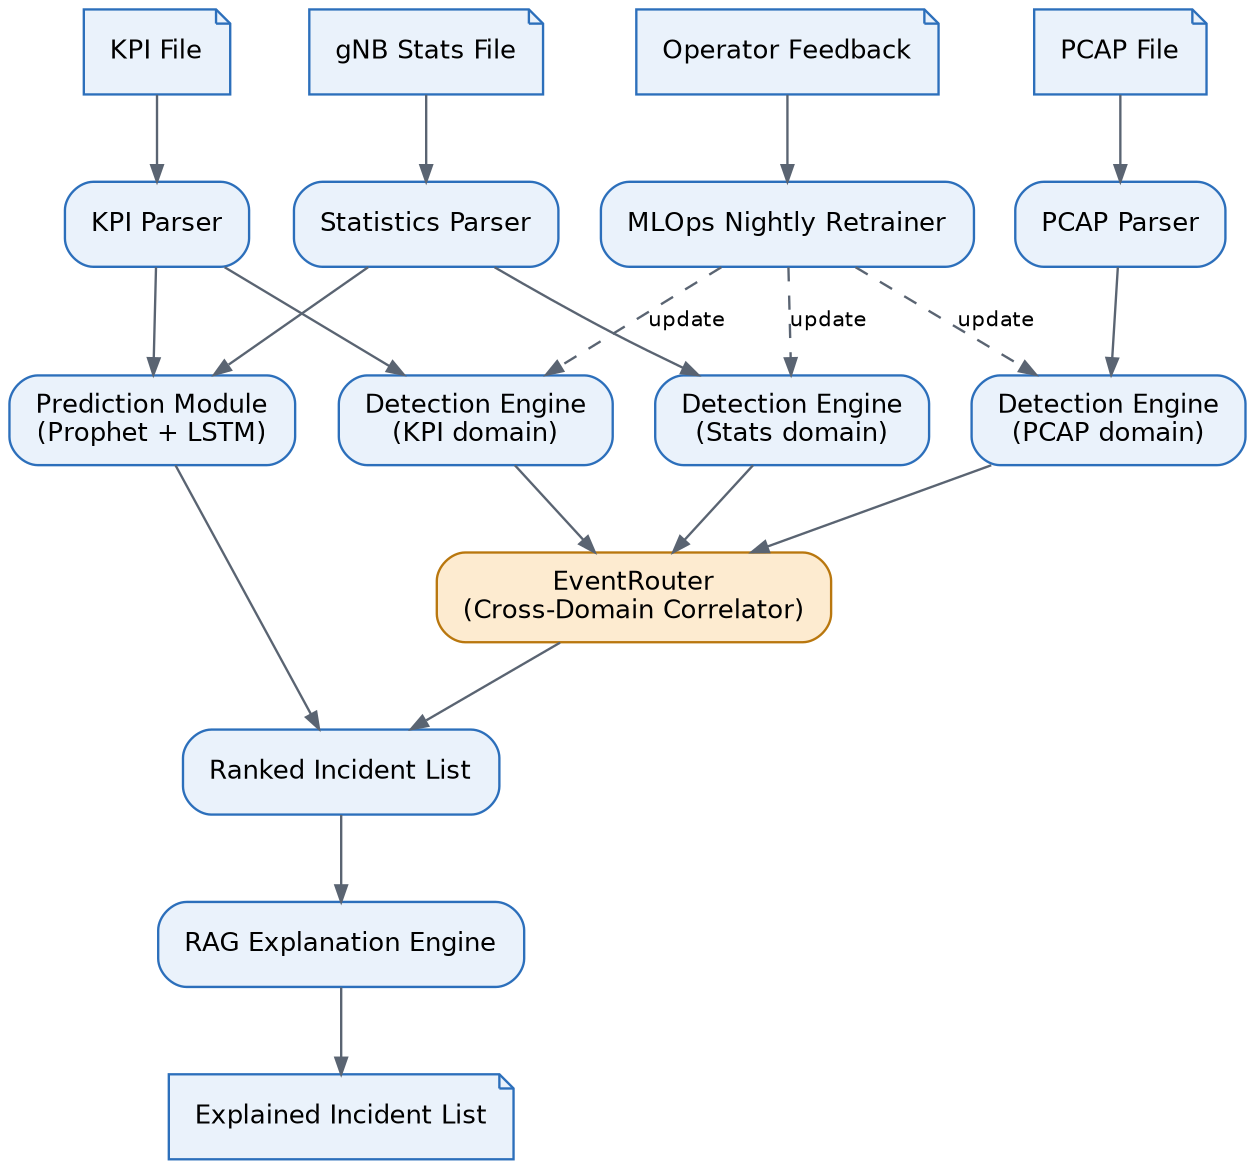
\includegraphics[width=0.85\textwidth]{figures/fig_5_1.png}
    \caption{Unified Pipeline End-to-End Control Flow --- End-to-end control flow of the Unified Telecom Analyzer, showing the Parse to Detect to Correlate to Explain pipeline with parallel Prediction and MLOps feedback branches.}
    \label{fig:5_1}
\end{figure}

\begin{figure}[htbp]
    \centering
    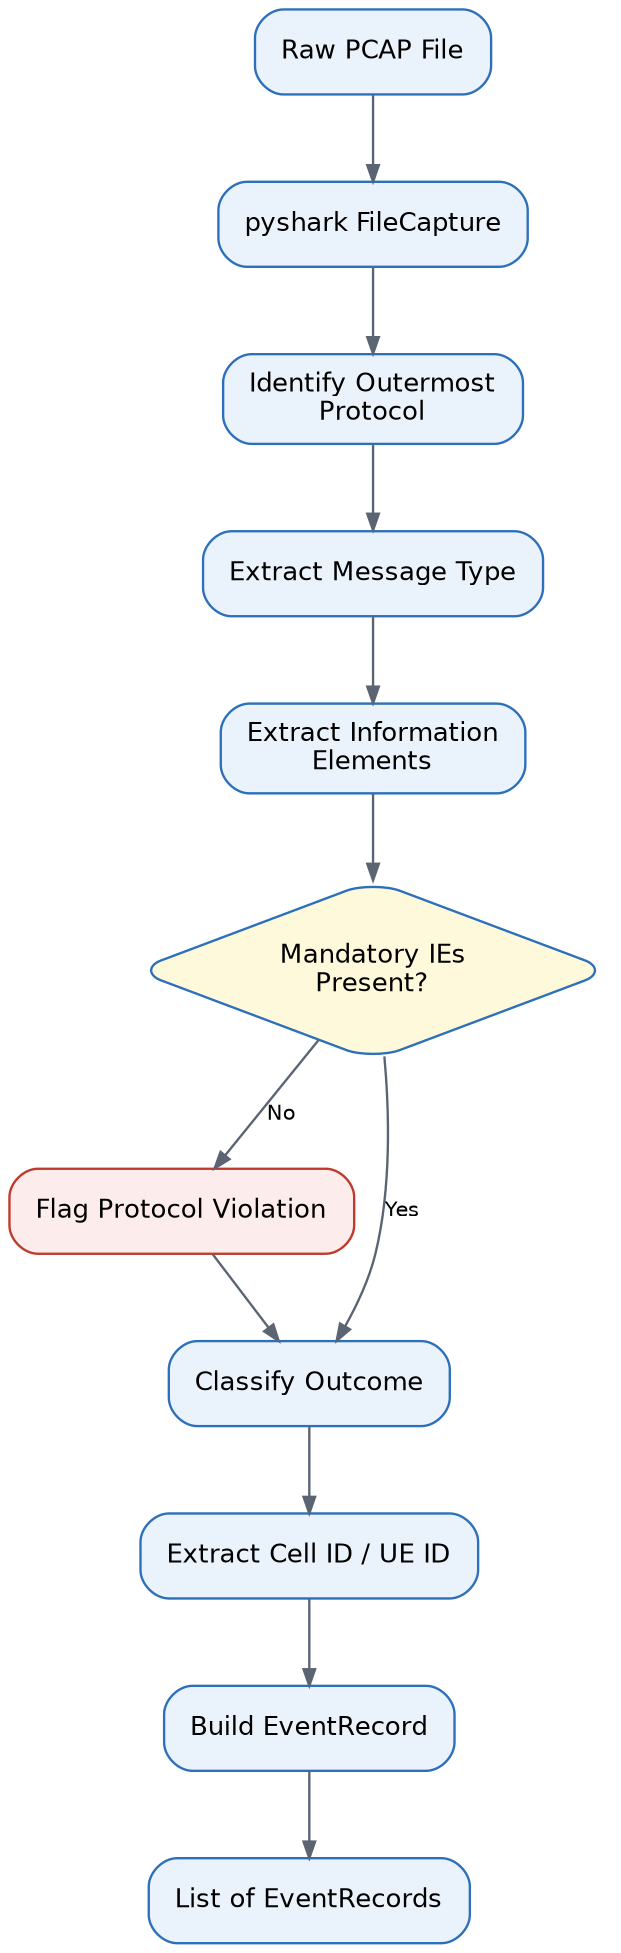
\includegraphics[width=0.85\textwidth]{figures/fig_5_2.png}
    \caption{PCAP Parser Workflow --- PCAP Parser processing workflow, including the spec-alignment branch that flags protocol violations independently of the anomaly ensemble.}
    \label{fig:5_2}
\end{figure}

\begin{figure}[htbp]
    \centering
    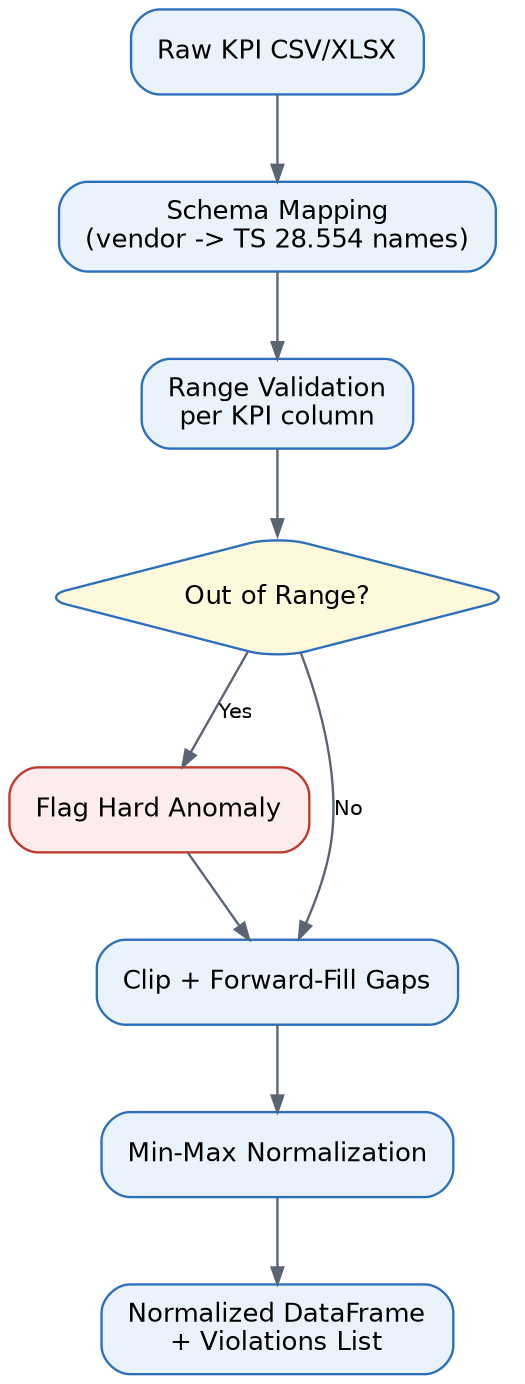
\includegraphics[width=0.85\textwidth]{figures/fig_5_3.png}
    \caption{KPI Parser Three-Stage Pipeline --- KPI Parser three-stage processing pipeline: schema mapping, range validation, and normalization.}
    \label{fig:5_3}
\end{figure}

\begin{figure}[htbp]
    \centering
    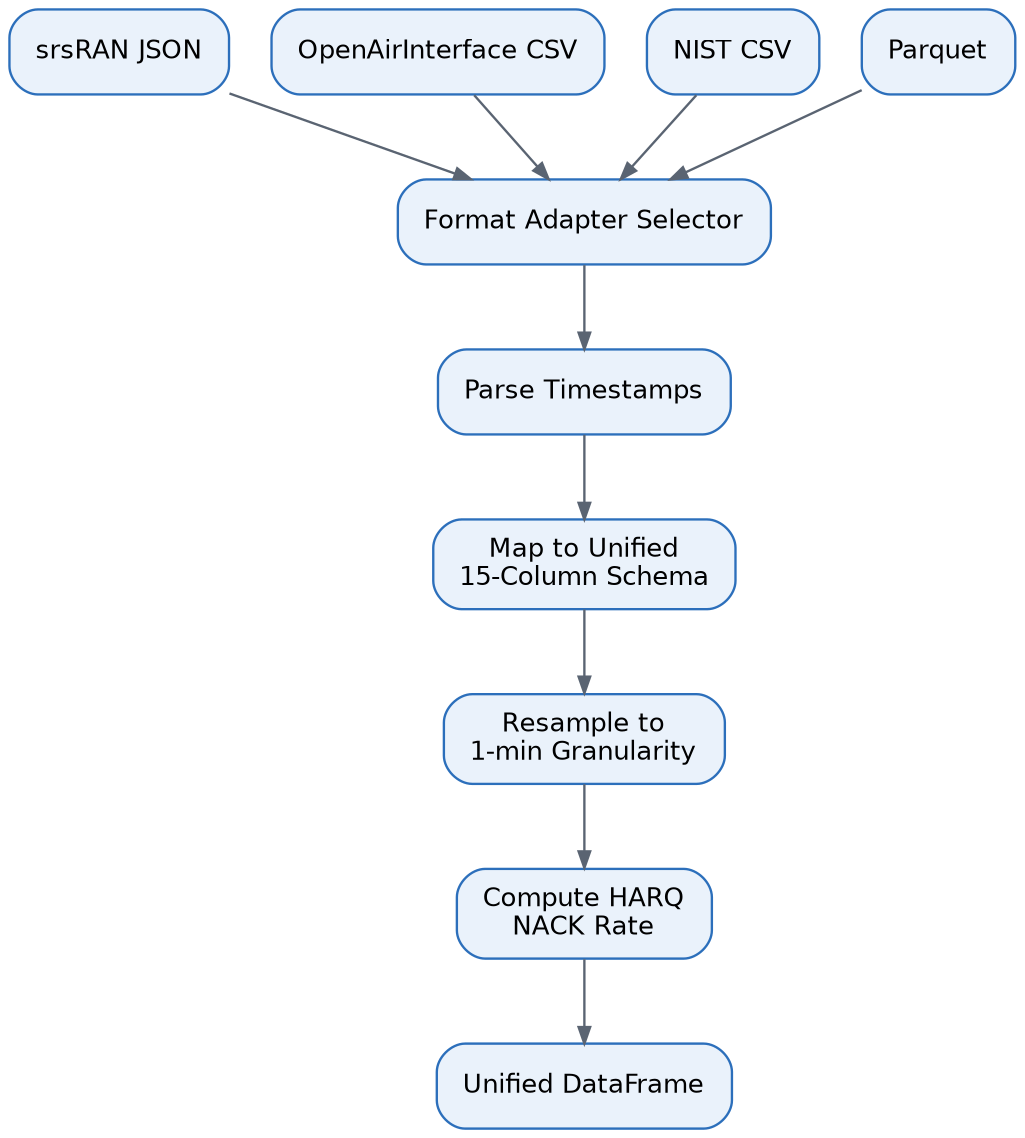
\includegraphics[width=0.85\textwidth]{figures/fig_5_4.png}
    \caption{Statistics Parser Multi-Format Adapter Architecture --- Statistics Parser adapter architecture unifying four input formats into a single 15-column schema.}
    \label{fig:5_4}
\end{figure}

\begin{figure}[htbp]
    \centering
    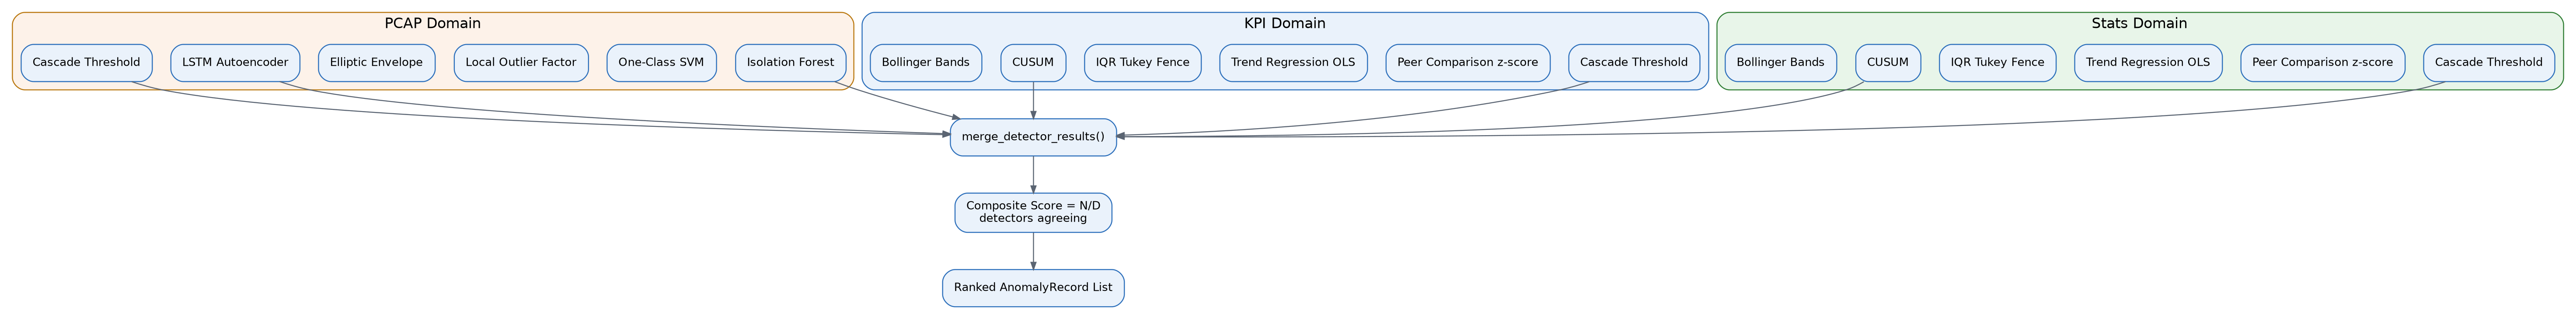
\includegraphics[width=0.85\textwidth]{figures/fig_5_5.png}
    \caption{18-Detector Ensemble Architecture --- 18-detector ensemble architecture: six algorithm families instantiated across three data domains, merged into a composite severity score.}
    \label{fig:5_5}
\end{figure}

\begin{figure}[htbp]
    \centering
    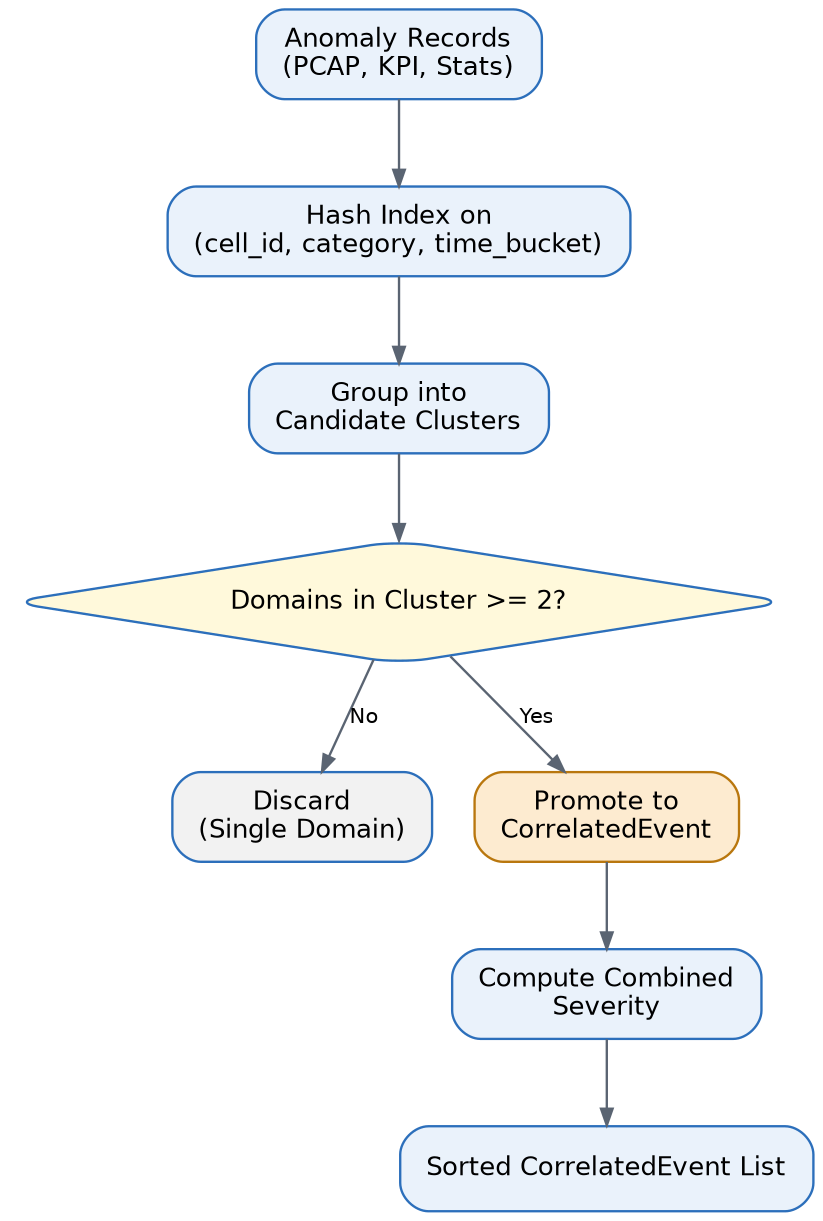
\includegraphics[width=0.85\textwidth]{figures/fig_5_6.png}
    \caption{EventRouter Cross-Domain Correlation --- EventRouter cross-domain correlation mechanism, promoting multi-domain anomaly clusters to CorrelatedEvents.}
    \label{fig:5_6}
\end{figure}

\begin{figure}[htbp]
    \centering
    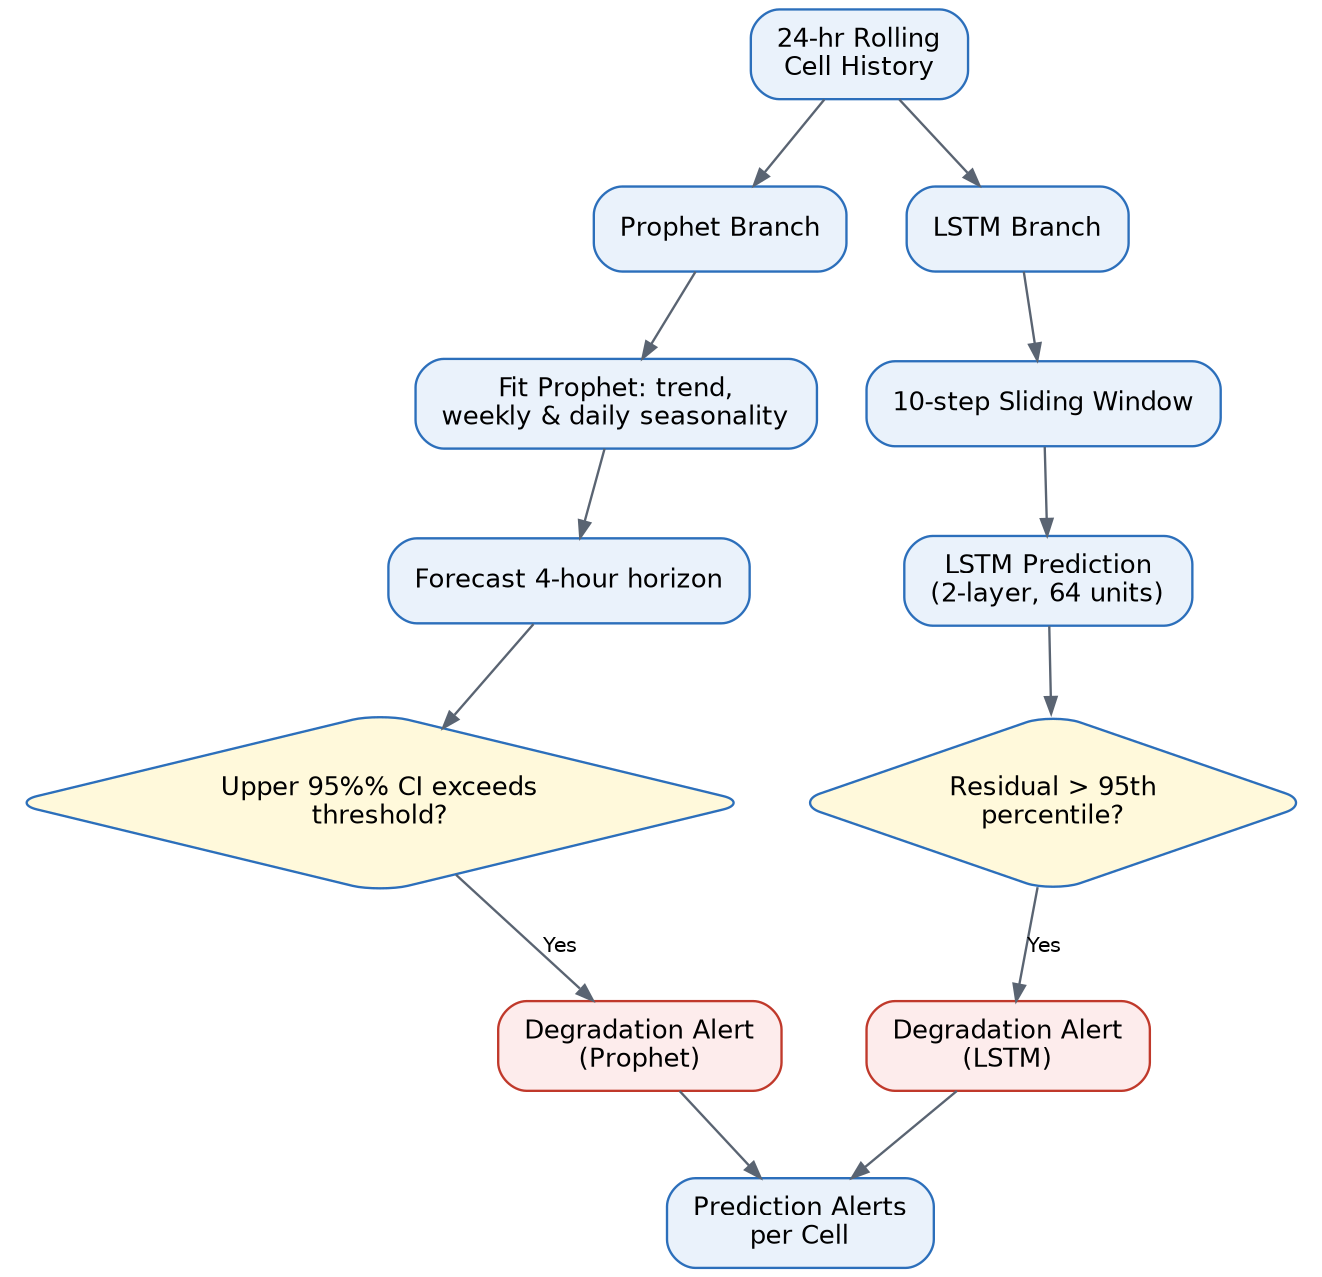
\includegraphics[width=0.85\textwidth]{figures/fig_5_7.png}
    \caption{Prediction Module Dual-Branch Design --- Dual-branch Prediction Module combining Prophet (seasonal patterns) and LSTM (non-linear sudden onset).}
    \label{fig:5_7}
\end{figure}

\begin{figure}[htbp]
    \centering
    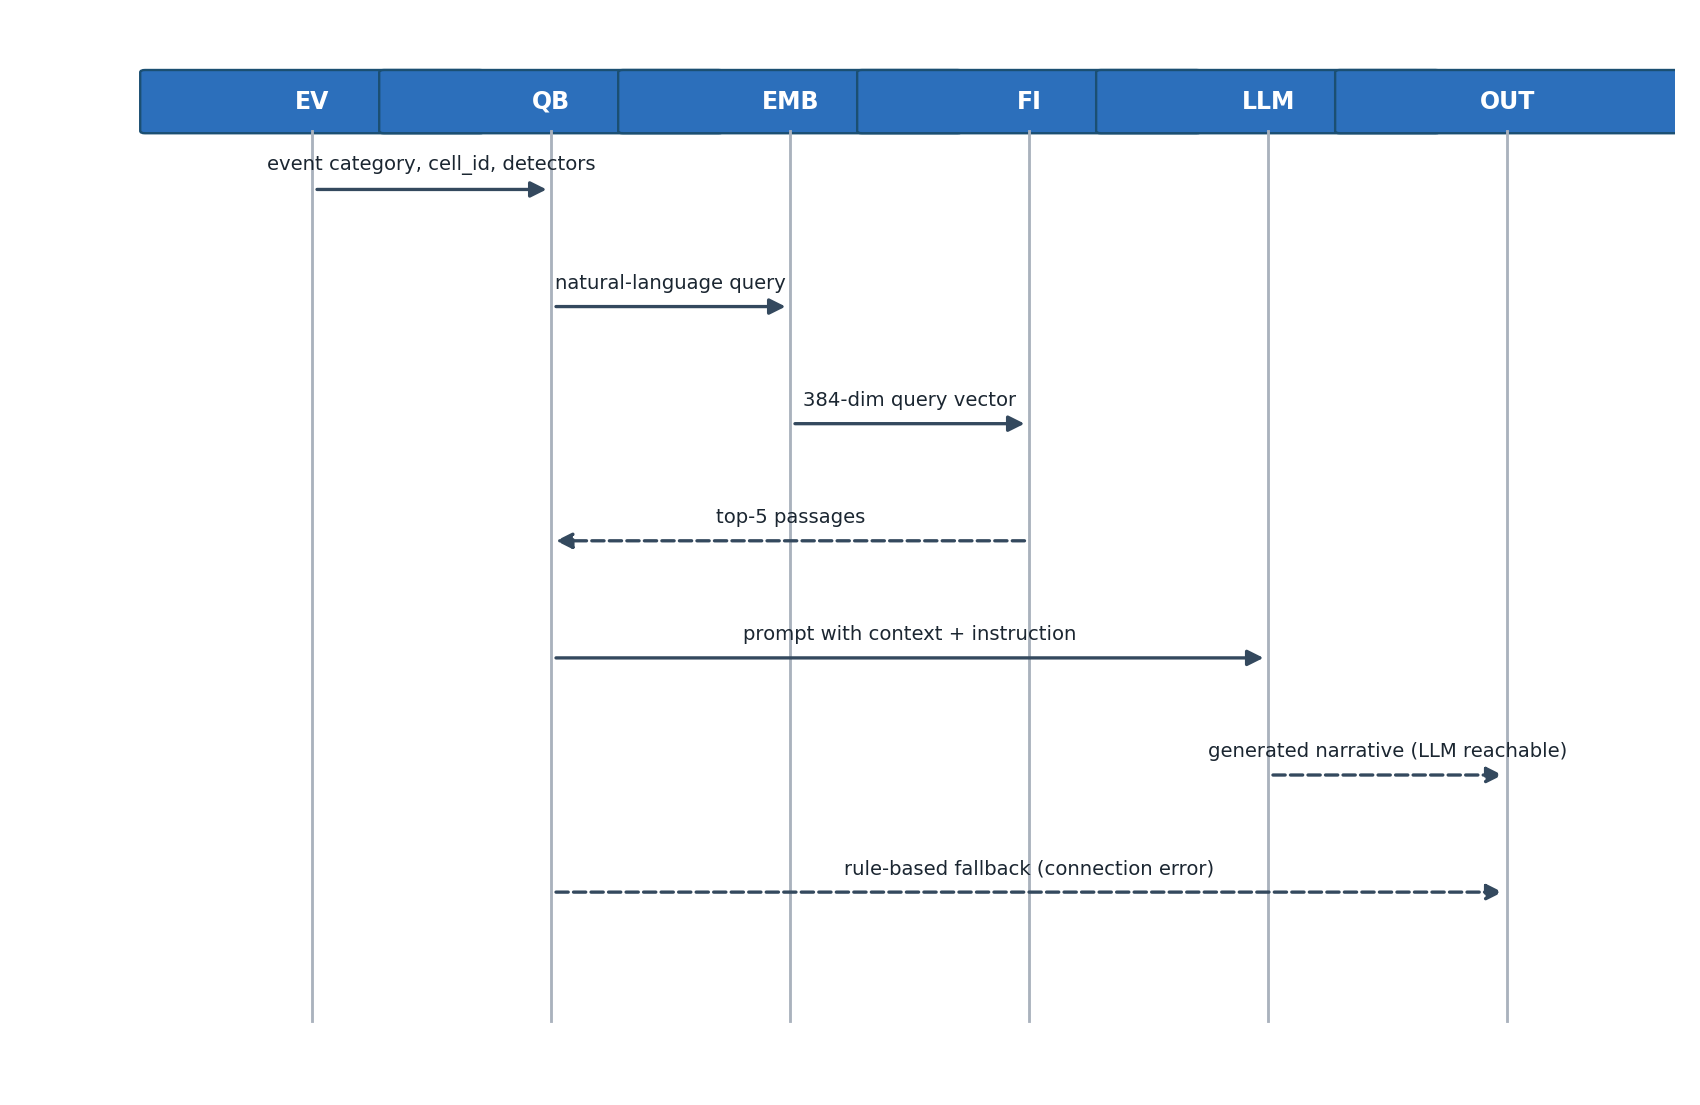
\includegraphics[width=0.85\textwidth]{figures/fig_5_8.png}
    \caption{RAG Explanation Engine Flow --- RAG Explanation Engine pipeline: query construction, FAISS retrieval, and LLM generation with offline fallback.}
    \label{fig:5_8}
\end{figure}

\begin{figure}[htbp]
    \centering
    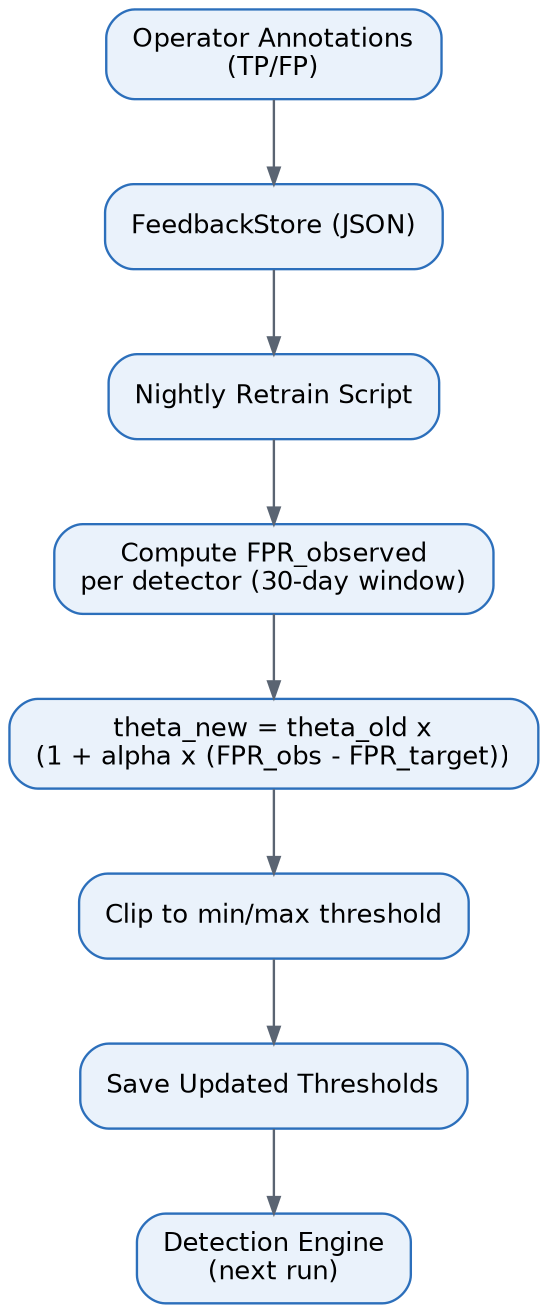
\includegraphics[width=0.85\textwidth]{figures/fig_5_9.png}
    \caption{MLOps Nightly Feedback Loop --- MLOps nightly feedback loop adjusting per-detector thresholds from operator false-positive annotations.}
    \label{fig:5_9}
\end{figure}

\begin{figure}[htbp]
    \centering
    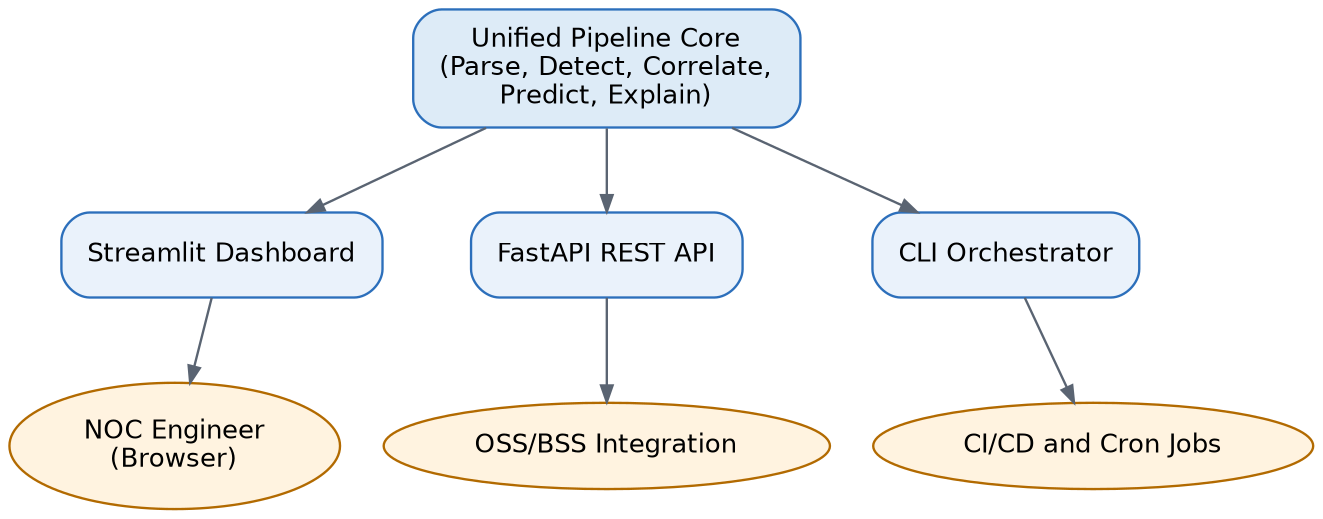
\includegraphics[width=0.85\textwidth]{figures/fig_5_10.png}
    \caption{Three Access Interfaces --- Three access interfaces (Dashboard, REST API, CLI) built on a shared pipeline core.}
    \label{fig:5_10}
\end{figure}

\begin{figure}[htbp]
    \centering
    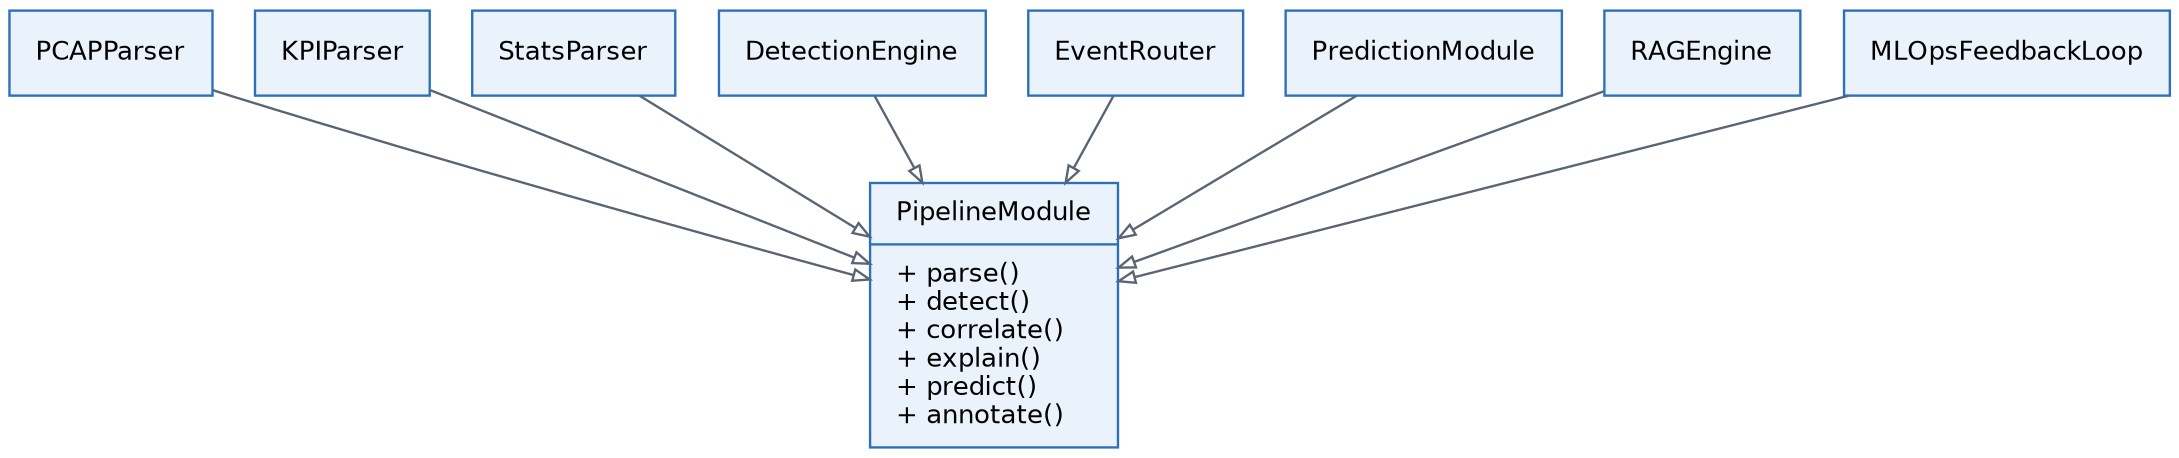
\includegraphics[width=0.85\textwidth]{figures/fig_5_11.png}
    \caption{Common Module Interface (Separation of Concerns) --- Common module interface enabling independent testing and future substitution of any pipeline component.}
    \label{fig:5_11}
\end{figure}

% ---------------- Chapter 6 ----------------
\begin{figure}[htbp]
    \centering
    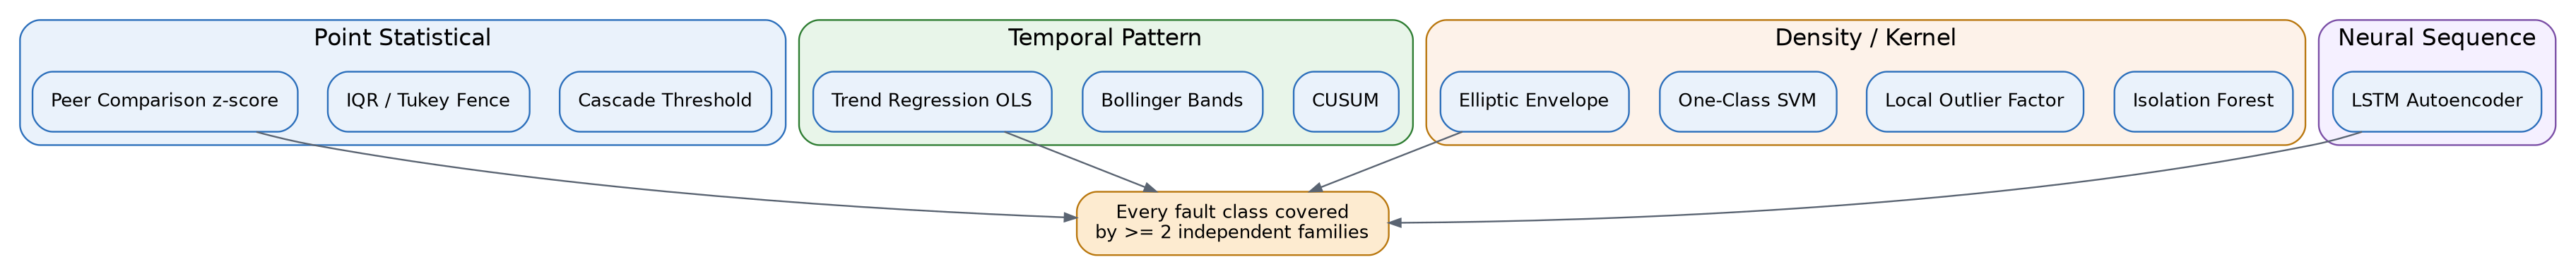
\includegraphics[width=0.85\textwidth]{figures/fig_6_1.png}
    \caption{Detector Family Taxonomy (Ensemble Coverage Principle) --- The twelve detection algorithms partitioned into four orthogonal families, the theoretical basis for the ensemble's fault-class coverage.}
    \label{fig:6_1}
\end{figure}

% ---------------- Chapter 7 ----------------
\begin{figure}[htbp]
    \centering
    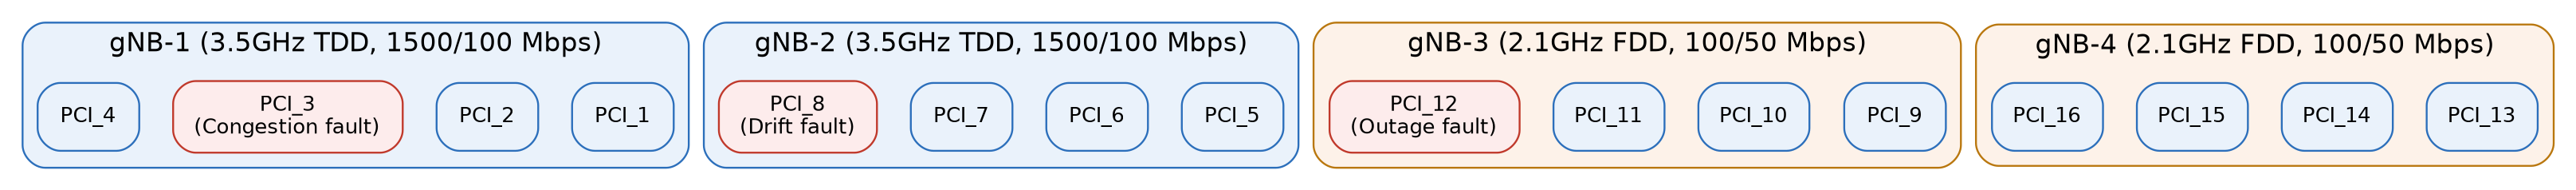
\includegraphics[width=0.85\textwidth]{figures/fig_7_1.png}
    \caption{Evaluation Network Topology --- Evaluation testbed topology: 4 gNBs / 16 cells / 64 UEs, with the three fault-injection cells highlighted.}
    \label{fig:7_1}
\end{figure}

\begin{figure}[htbp]
    \centering
    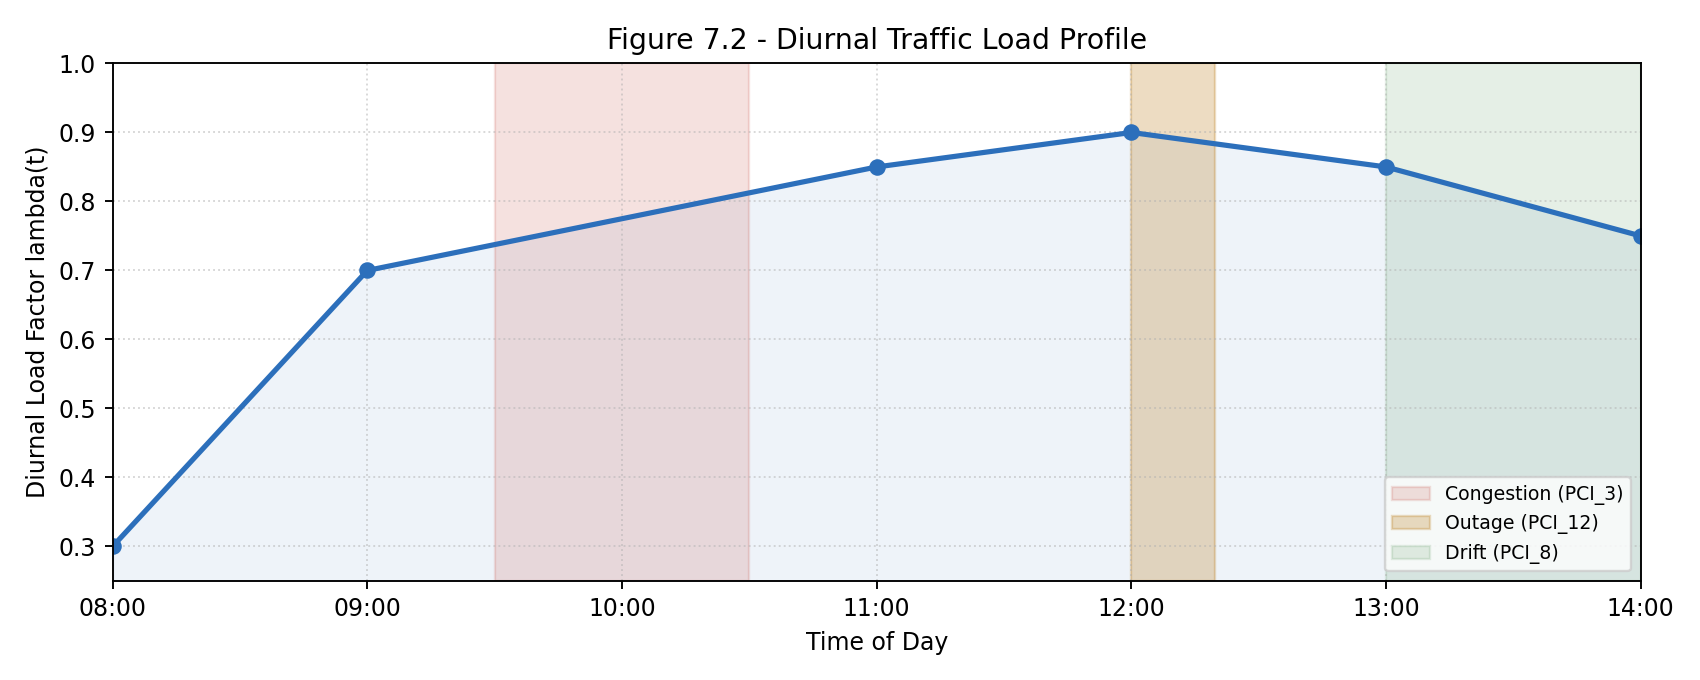
\includegraphics[width=0.85\textwidth]{figures/fig_7_2.png}
    \caption{Diurnal Traffic Load Profile --- Diurnal load factor over the 6-hour simulation window, with the three fault-injection windows marked.}
    \label{fig:7_2}
\end{figure}

\begin{figure}[htbp]
    \centering
    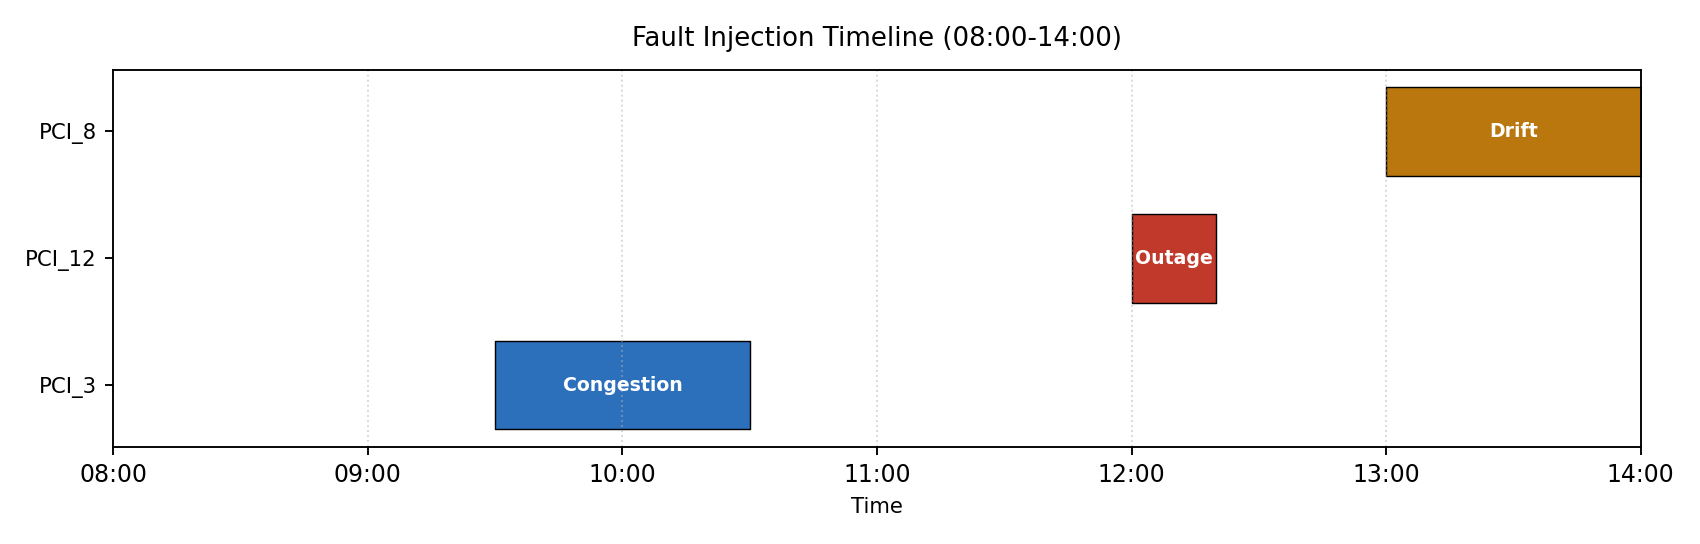
\includegraphics[width=0.85\textwidth]{figures/fig_7_3.png}
    \caption{Fault Injection Timeline --- Timeline of the three concurrent injected fault scenarios across the 6-hour evaluation window.}
    \label{fig:7_3}
\end{figure}

\begin{figure}[htbp]
    \centering
    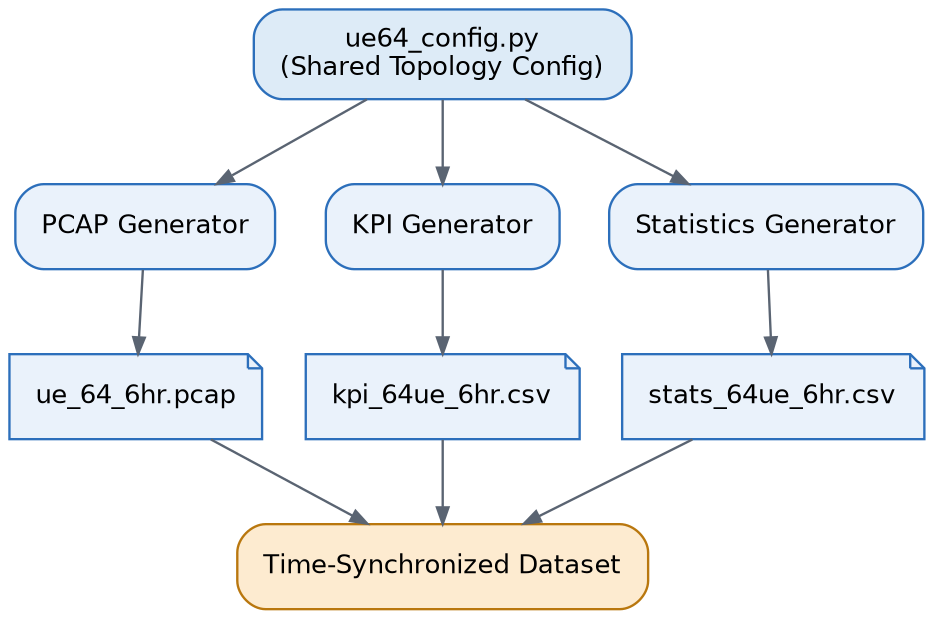
\includegraphics[width=0.85\textwidth]{figures/fig_7_4.png}
    \caption{Dataset Generation Pipeline --- Synthetic dataset generation pipeline: a single shared topology configuration produces three time-synchronized, cross-domain-consistent data files.}
    \label{fig:7_4}
\end{figure}

% ---------------- Chapter 8 ----------------
\begin{figure}[htbp]
    \centering
    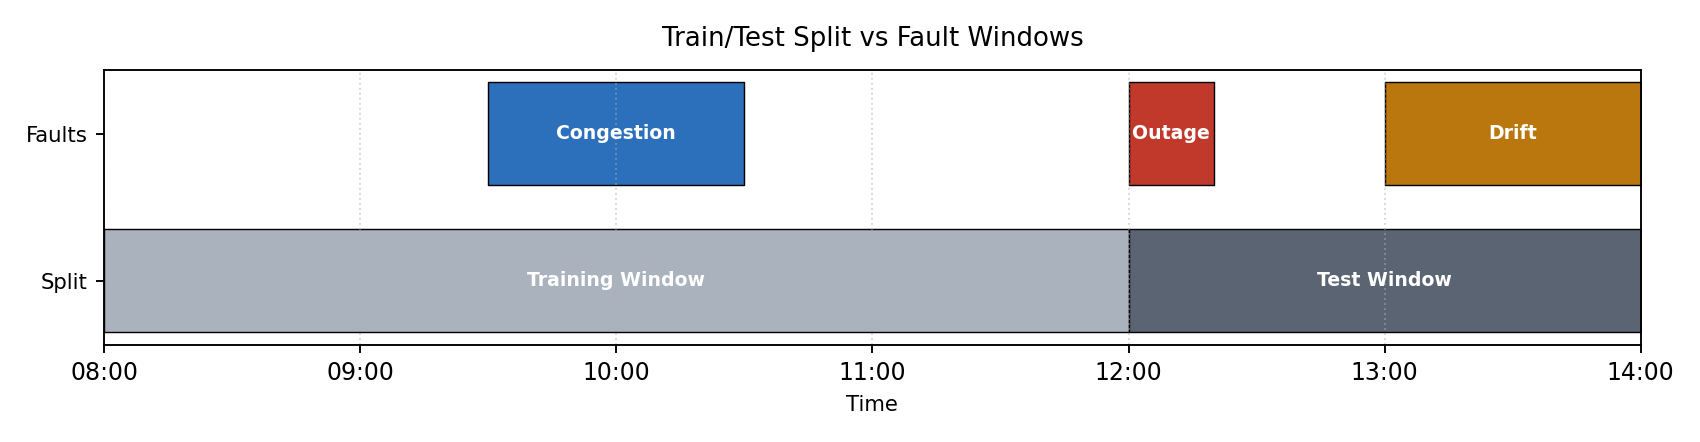
\includegraphics[width=0.85\textwidth]{figures/fig_8_1.png}
    \caption{Train/Test Temporal Split with Fault Overlay --- Temporal train/test split overlaid with the three fault windows, showing that the congestion fault straddles both windows while outage and drift fall entirely in the test window.}
    \label{fig:8_1}
\end{figure}

% ---------------- Chapter 9 ----------------
\begin{figure}[htbp]
    \centering
    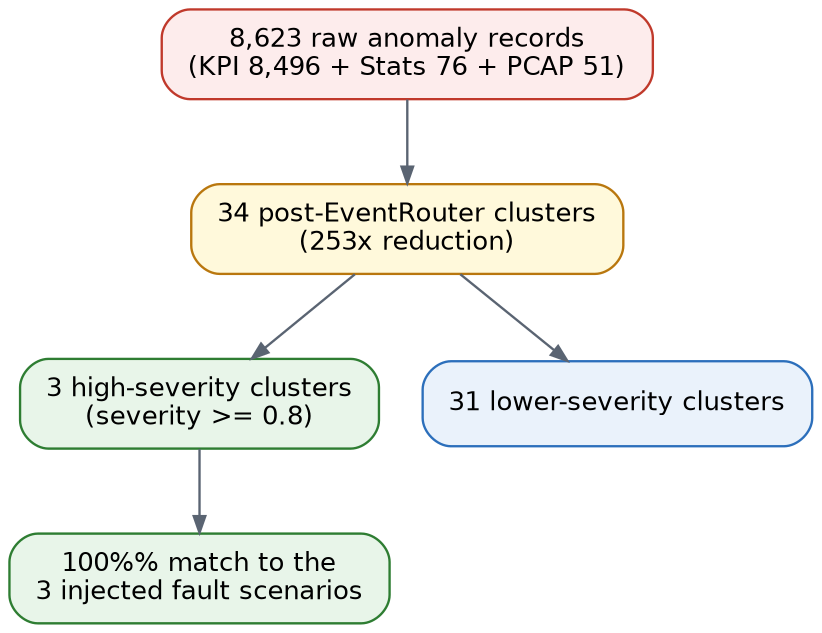
\includegraphics[width=0.85\textwidth]{figures/fig_9_1.png}
    \caption{EventRouter Alarm-Volume Reduction Funnel --- Alarm-volume reduction achieved by the EventRouter: 8,623 raw records collapse to 34 operator-visible clusters, with all three high-severity clusters correctly matching the injected faults.}
    \label{fig:9_1}
\end{figure}

\begin{figure}[htbp]
    \centering
    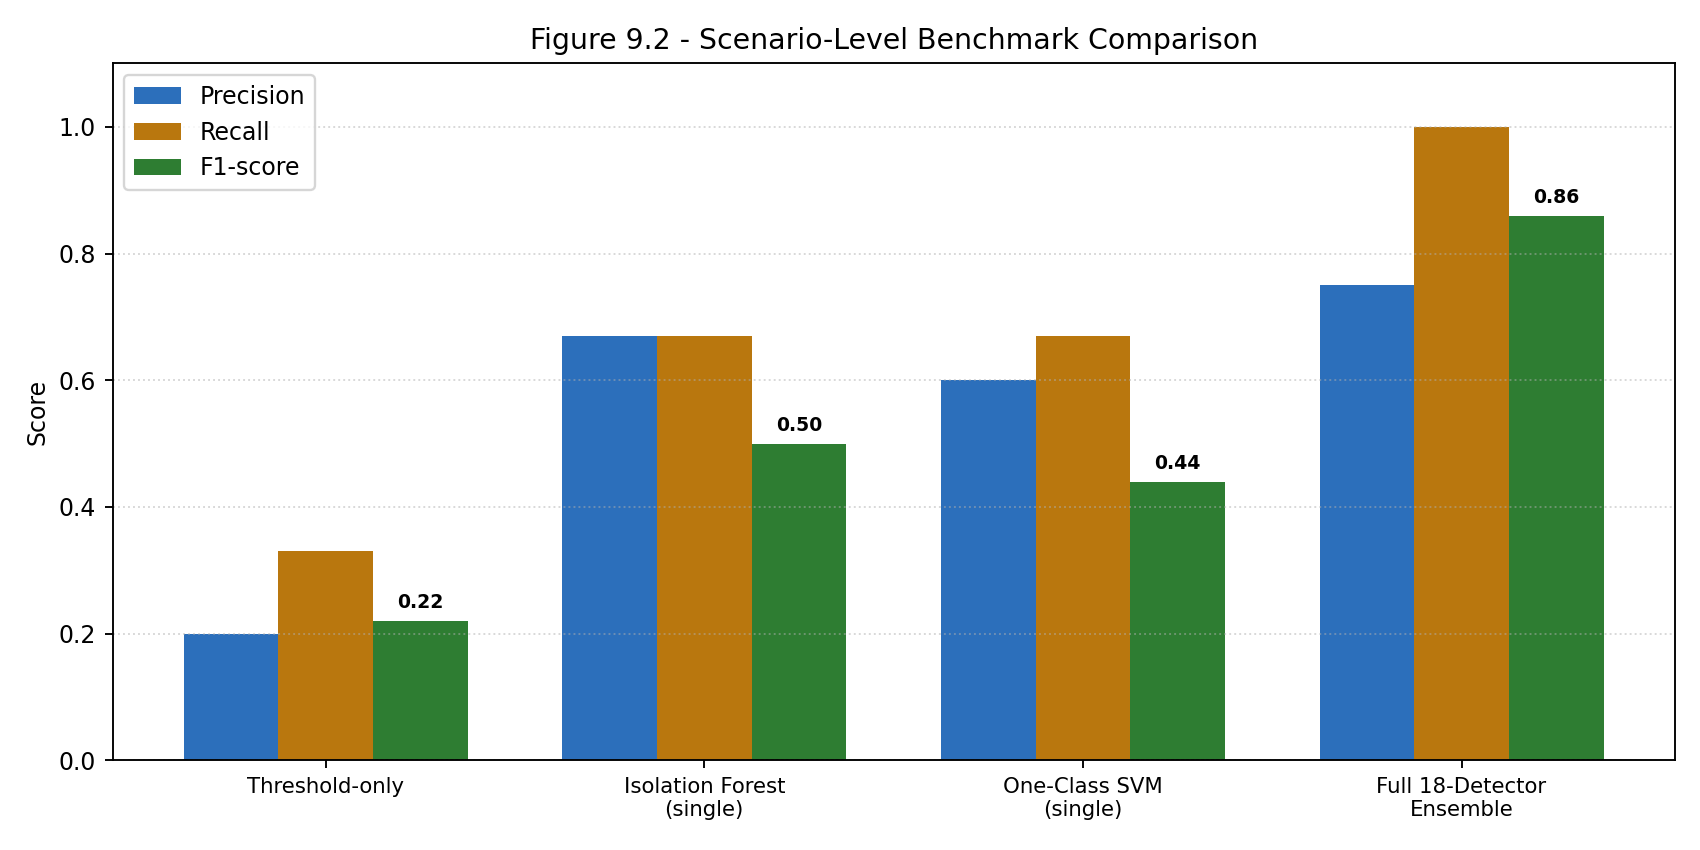
\includegraphics[width=0.85\textwidth]{figures/fig_9_2.png}
    \caption{Benchmark Comparison (Precision/Recall/F1) --- Scenario-level Precision, Recall, and F1 across the threshold-only baseline, two single-detector baselines, and the full 18-detector ensemble.}
    \label{fig:9_2}
\end{figure}

\begin{figure}[htbp]
    \centering
    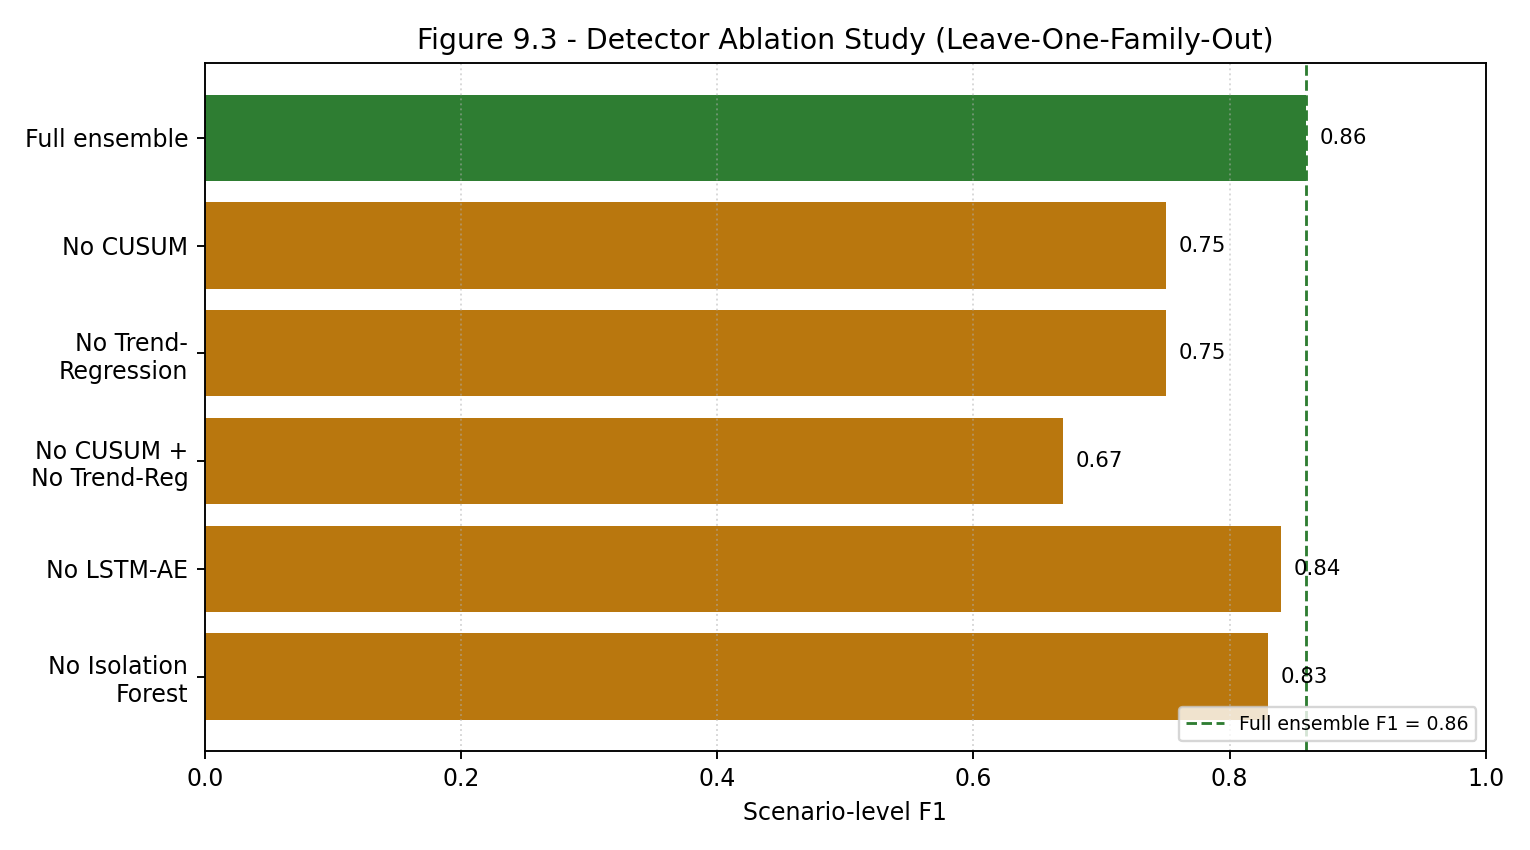
\includegraphics[width=0.85\textwidth]{figures/fig_9_3.png}
    \caption{Detector Ablation Study --- Leave-one-family-out ablation results, showing CUSUM and Trend-Regression as jointly necessary for slow-drift detection.}
    \label{fig:9_3}
\end{figure}

\begin{figure}[htbp]
    \centering
    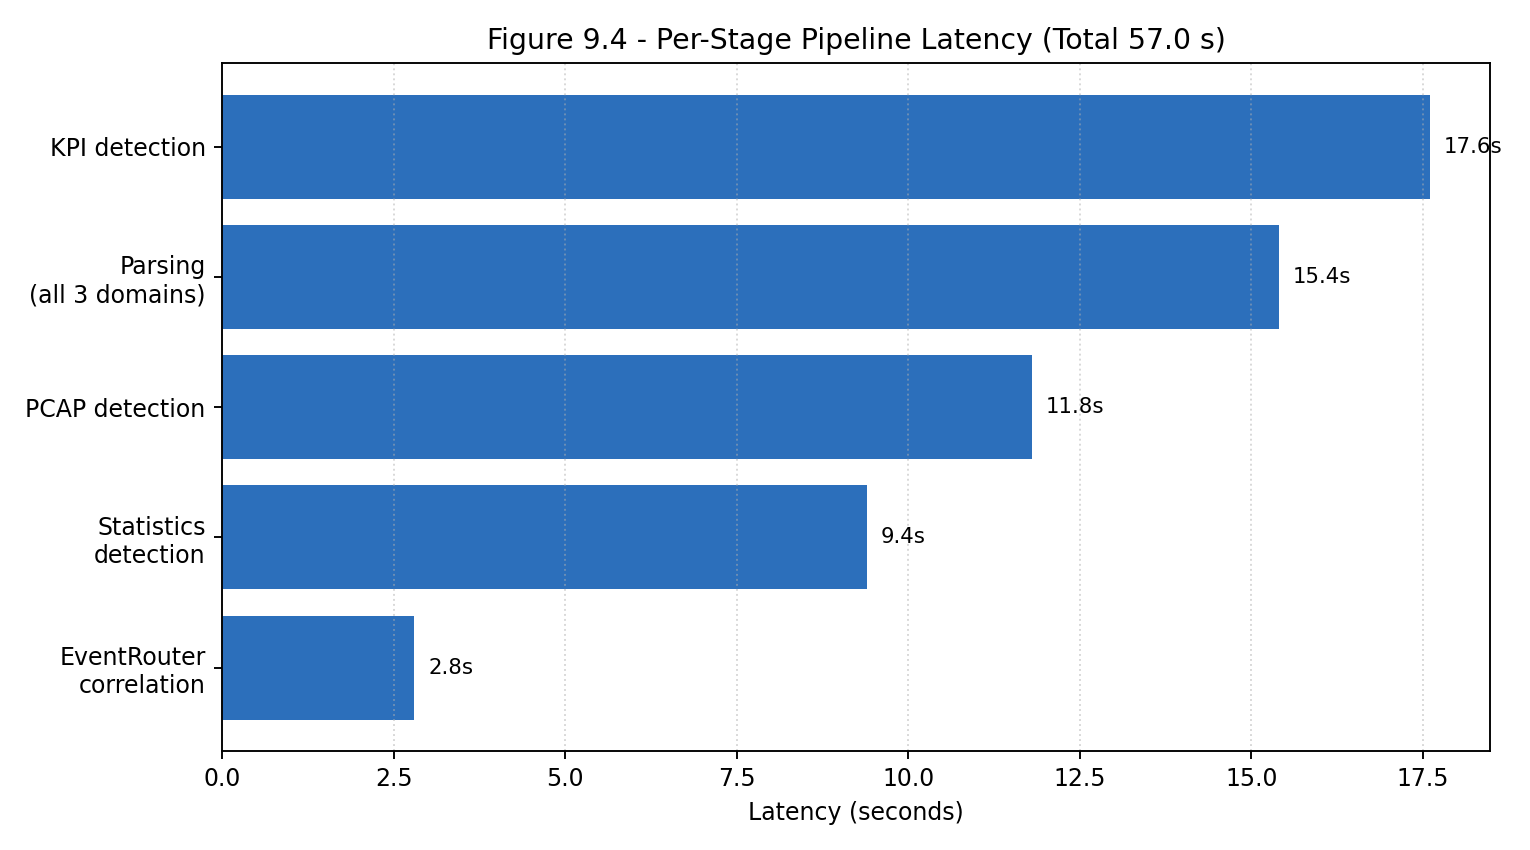
\includegraphics[width=0.85\textwidth]{figures/fig_9_4.png}
    \caption{Pipeline Latency Breakdown by Stage --- Per-stage latency breakdown of the 57-second end-to-end pipeline on the 64-UE dataset.}
    \label{fig:9_4}
\end{figure}

\begin{figure}[htbp]
    \centering
    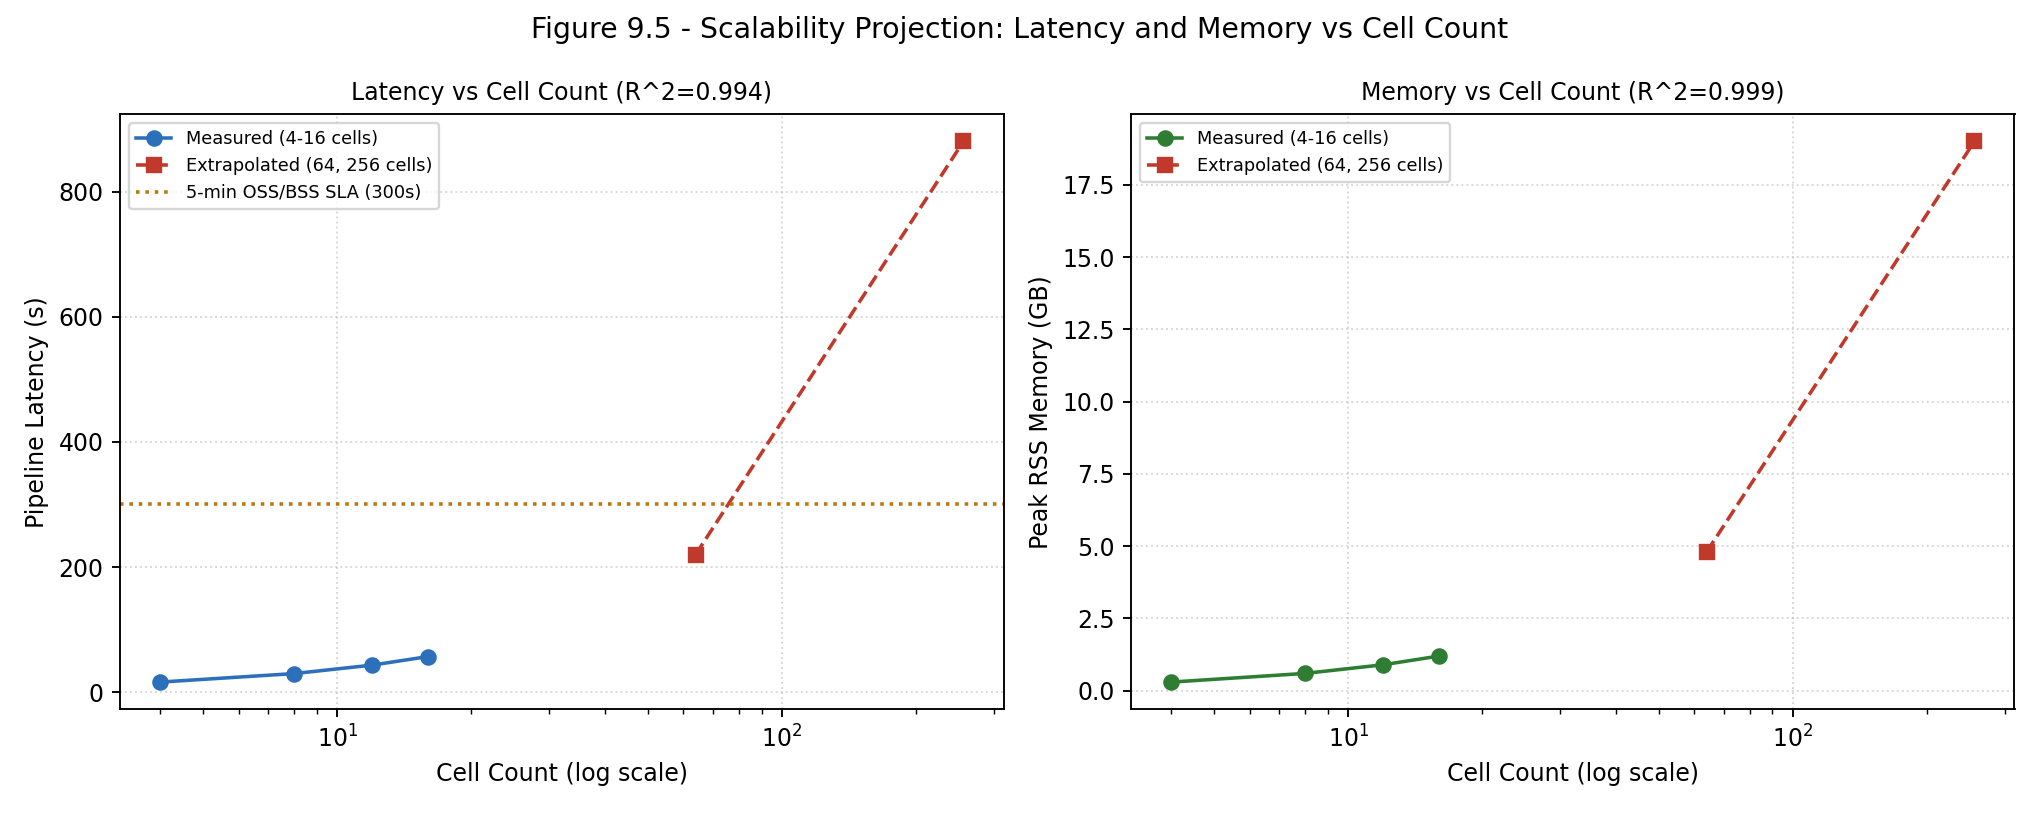
\includegraphics[width=0.85\textwidth]{figures/fig_9_5.png}
    \caption{Scalability Projection (Latency \& Memory vs. Cell Count) --- Measured (4 to 16 cells) and extrapolated (64, 256 cells) pipeline latency and peak memory, with the 5-minute OSS/BSS batch-cycle threshold marked.}
    \label{fig:9_5}
\end{figure}

% ---------------- Chapter 10 ----------------
\begin{figure}[htbp]
    \centering
    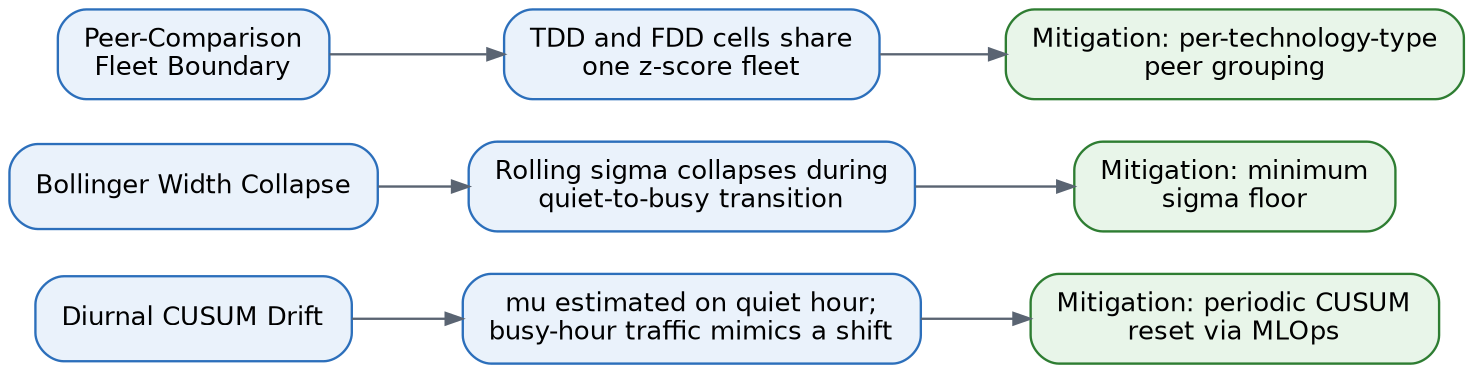
\includegraphics[width=0.85\textwidth]{figures/fig_10_1.png}
    \caption{False-Positive Root-Cause Map --- The three systematic sources of per-record false positives, their underlying mechanism, and the proposed mitigation for each.}
    \label{fig:10_1}
\end{figure}

% ---------------- Chapter 11 ----------------
\begin{figure}[htbp]
    \centering
    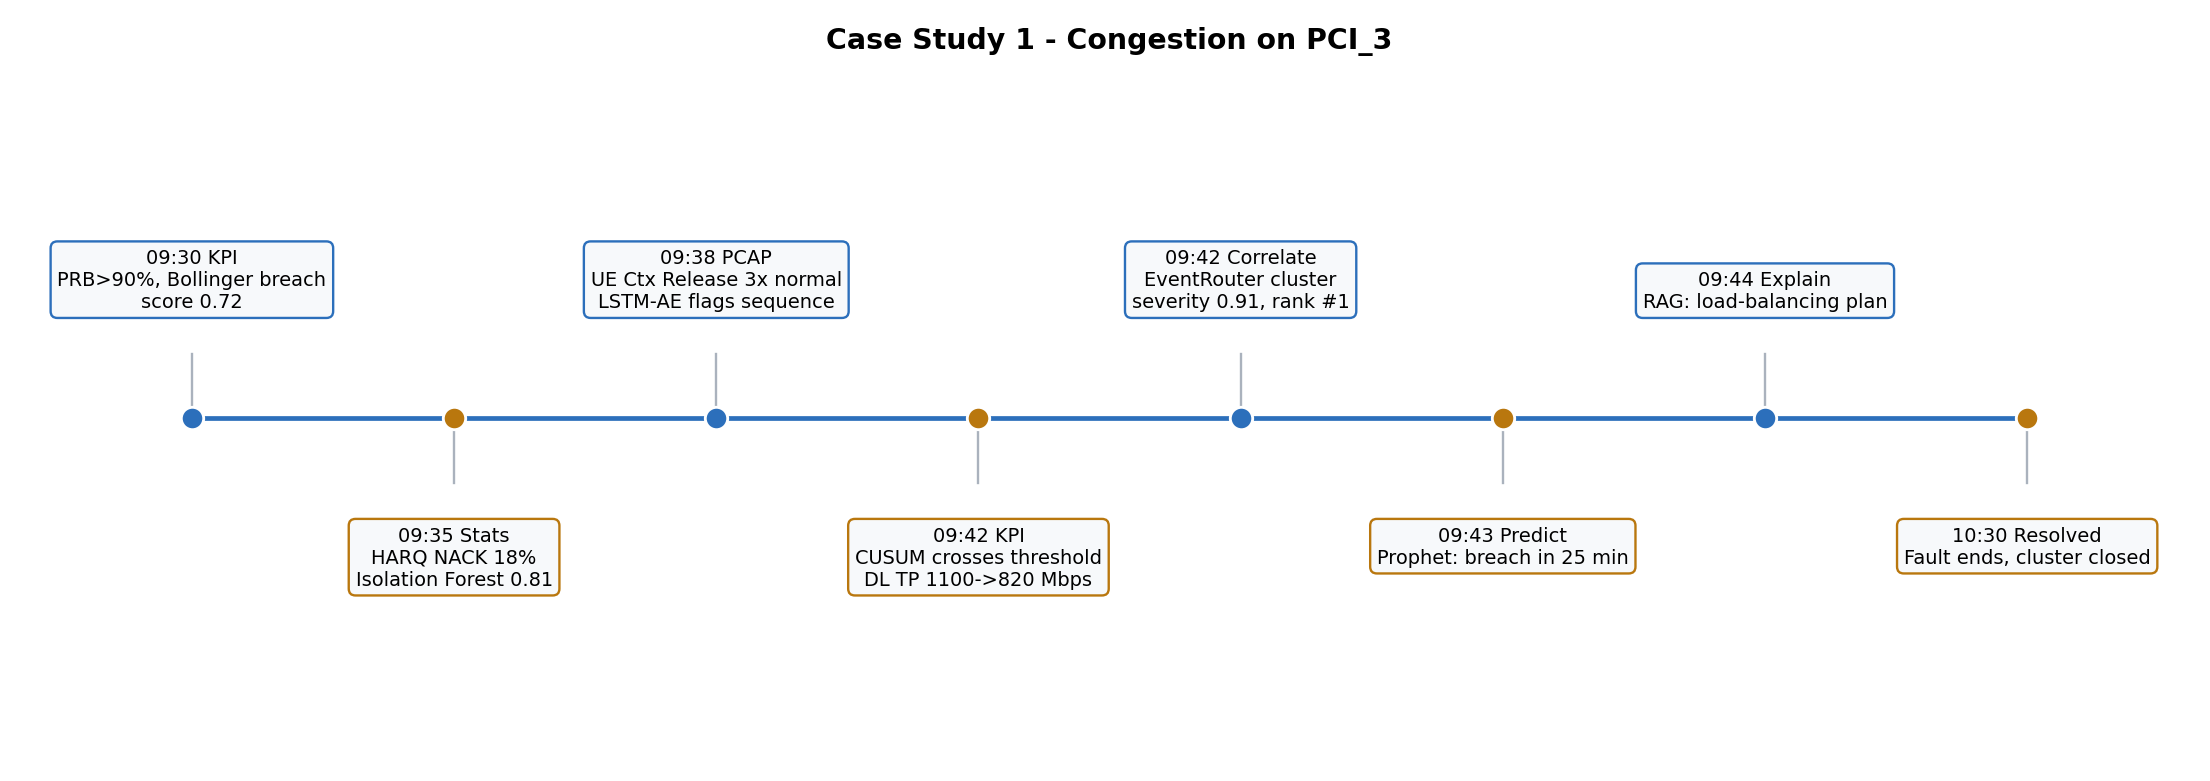
\includegraphics[width=0.85\textwidth]{figures/fig_11_1.png}
    \caption{Case Study 1 Timeline: Congestion on PCI_3 --- End-to-end pipeline trace for the PCI_3 congestion case study, from onset (09:30) to correlated detection (09:42) and explanation (09:44).}
    \label{fig:11_1}
\end{figure}

\begin{figure}[htbp]
    \centering
    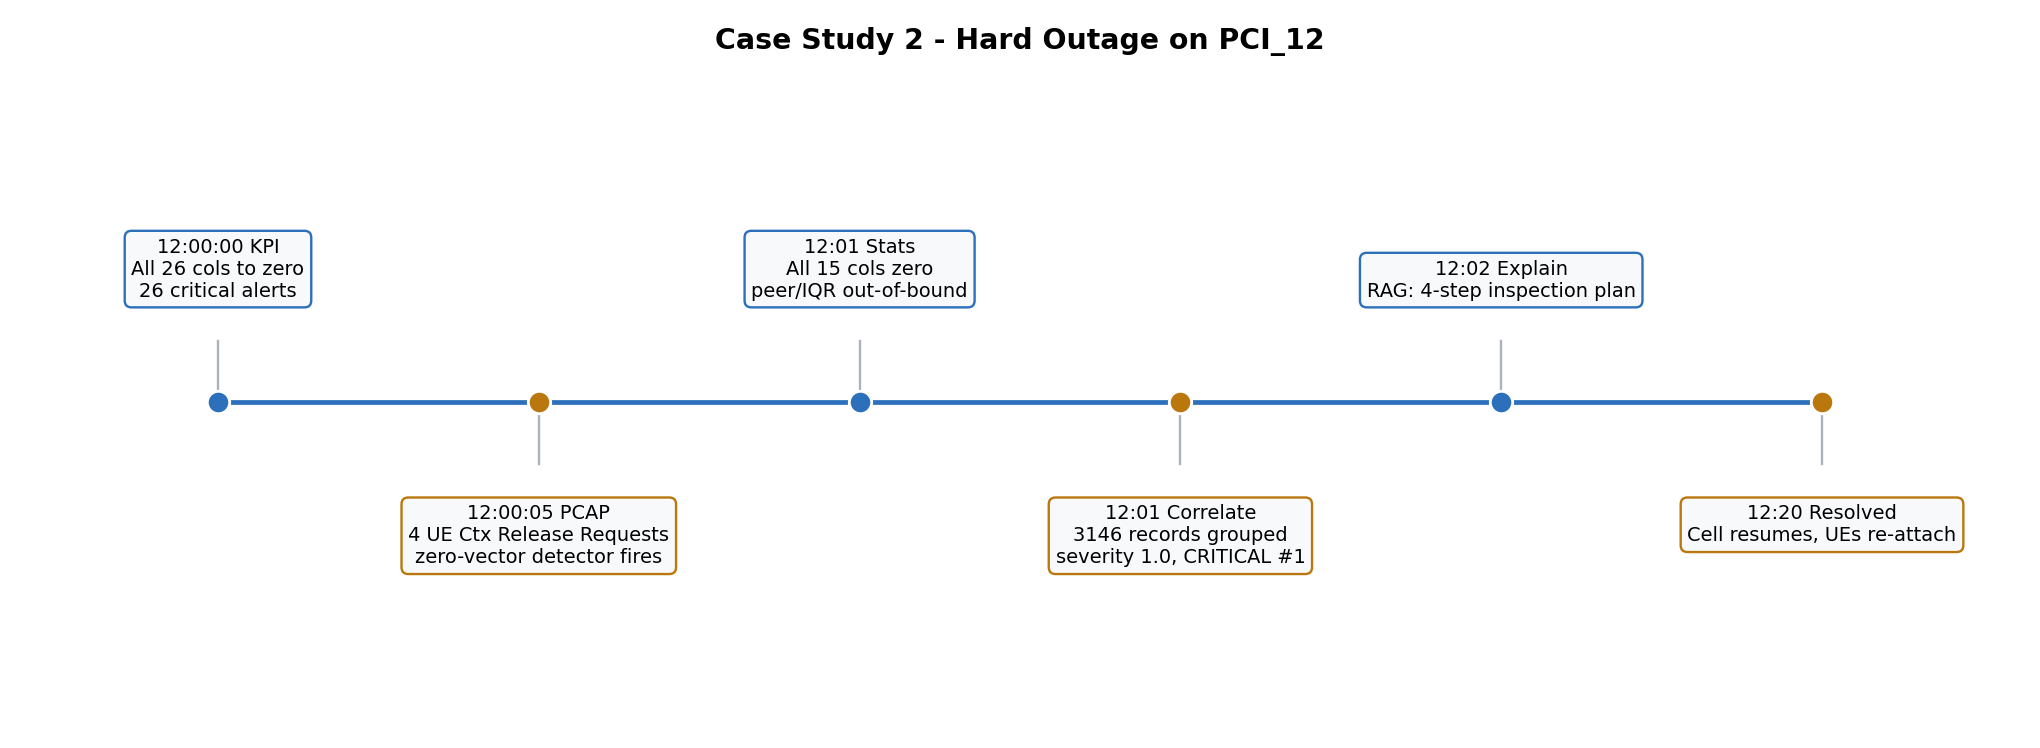
\includegraphics[width=0.85\textwidth]{figures/fig_11_2.png}
    \caption{Case Study 2 Timeline: Hard Outage on PCI_12 --- End-to-end pipeline trace for the PCI_12 hard outage, showing sub-minute detection and immediate severity-1.0 correlation.}
    \label{fig:11_2}
\end{figure}

\begin{figure}[htbp]
    \centering
    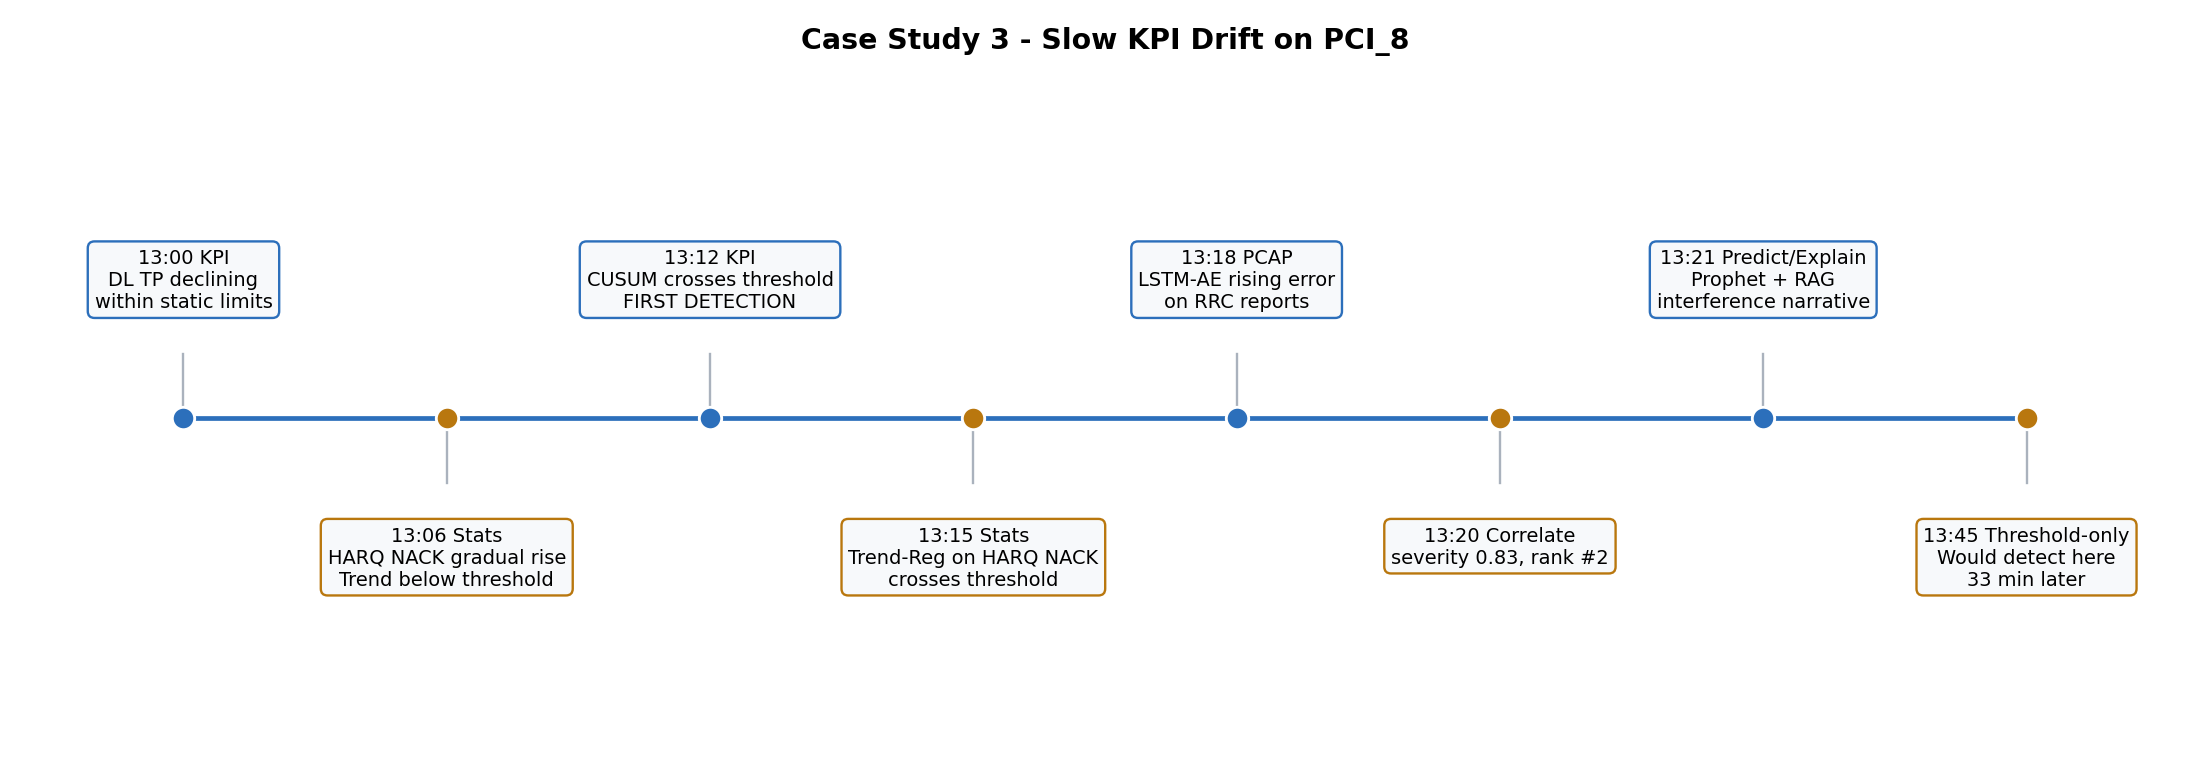
\includegraphics[width=0.85\textwidth]{figures/fig_11_3.png}
    \caption{Case Study 3 Timeline: Slow KPI Drift on PCI_8 --- End-to-end pipeline trace for the PCI_8 slow-drift case study, highlighting the 33-minute early-detection advantage of CUSUM over a threshold-only baseline.}
    \label{fig:11_3}
\end{figure}

% ---------------- Chapter 12 ----------------
\begin{figure}[htbp]
    \centering
    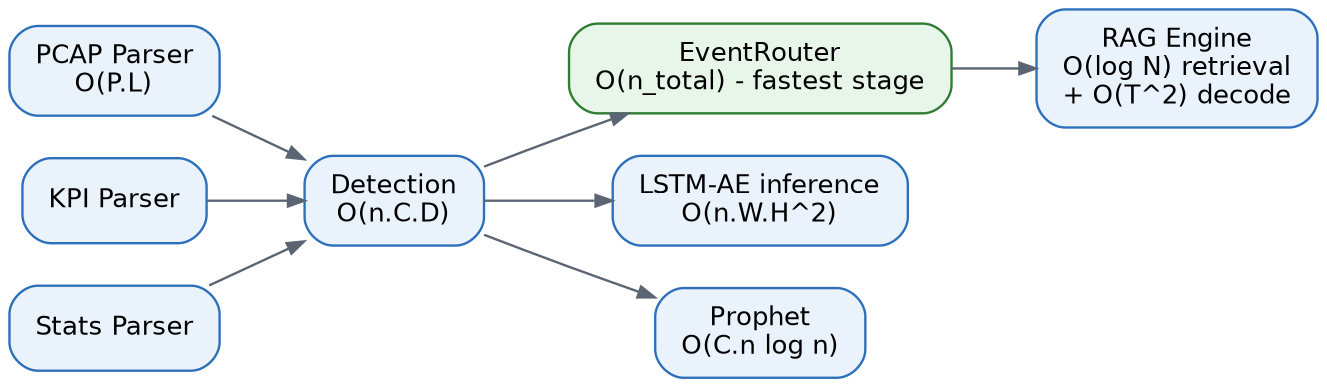
\includegraphics[width=0.85\textwidth]{figures/fig_12_1.png}
    \caption{Module-Level Complexity Overview --- Pipeline stages annotated with their asymptotic time complexity, showing the EventRouter as the fastest stage despite processing the largest input.}
    \label{fig:12_1}
\end{figure}

% ---------------- Chapter 14 ----------------
\begin{figure}[htbp]
    \centering
    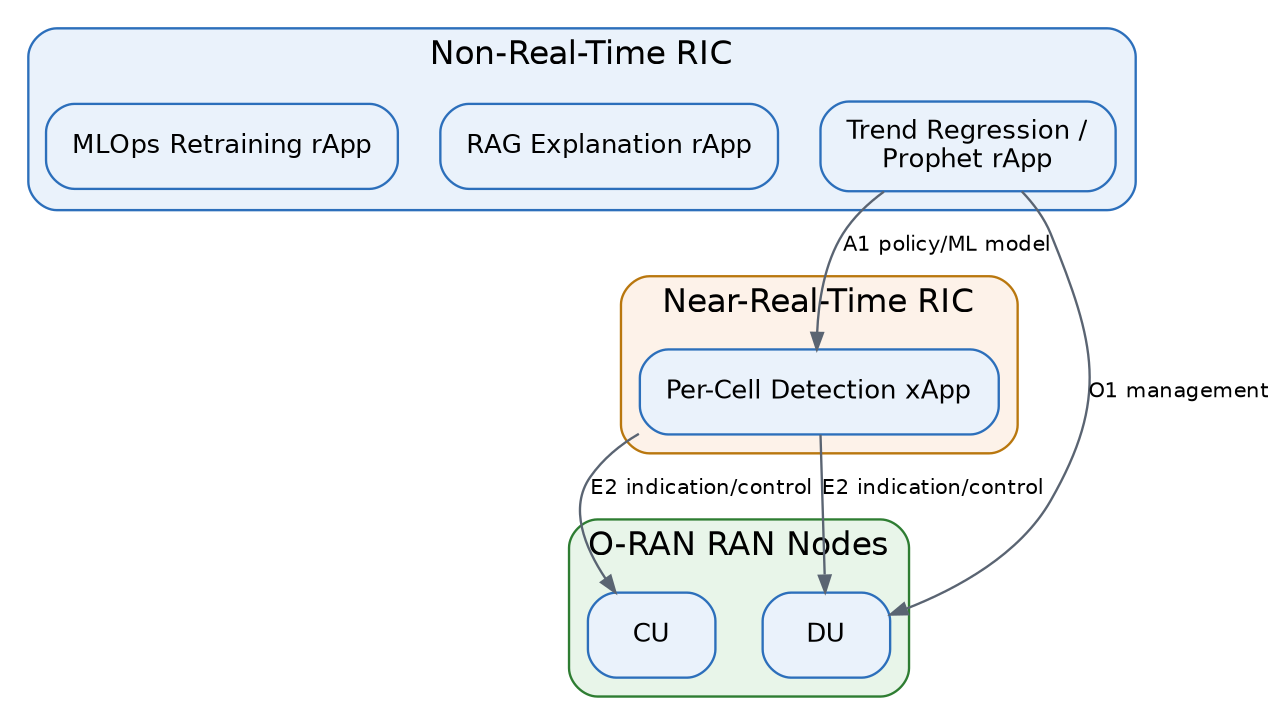
\includegraphics[width=0.85\textwidth]{figures/fig_14_1.png}
    \caption{O-RAN RIC Integration Architecture --- Mapping of the Unified Telecom Analyzer's pipeline modules onto the O-RAN Non-RT RIC (rApps) and Near-RT RIC (xApp) via the A1, O1, and E2 interfaces.}
    \label{fig:14_1}
\end{figure}

\begin{figure}[htbp]
    \centering
    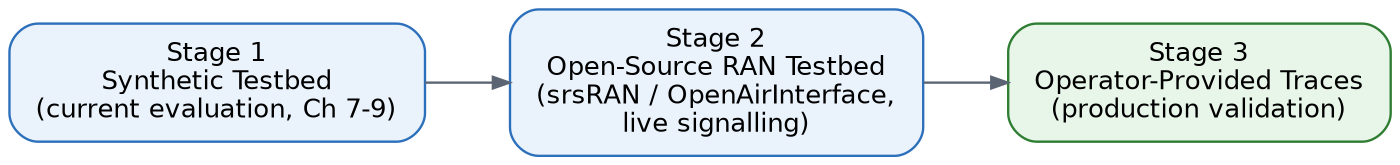
\includegraphics[width=0.85\textwidth]{figures/fig_14_2.png}
    \caption{Staged Production Validation Roadmap --- The staged validation path from the current synthetic evaluation to production deployment on operator traces.}
    \label{fig:14_2}
\end{figure}

\begin{figure}[htbp]
    \centering
    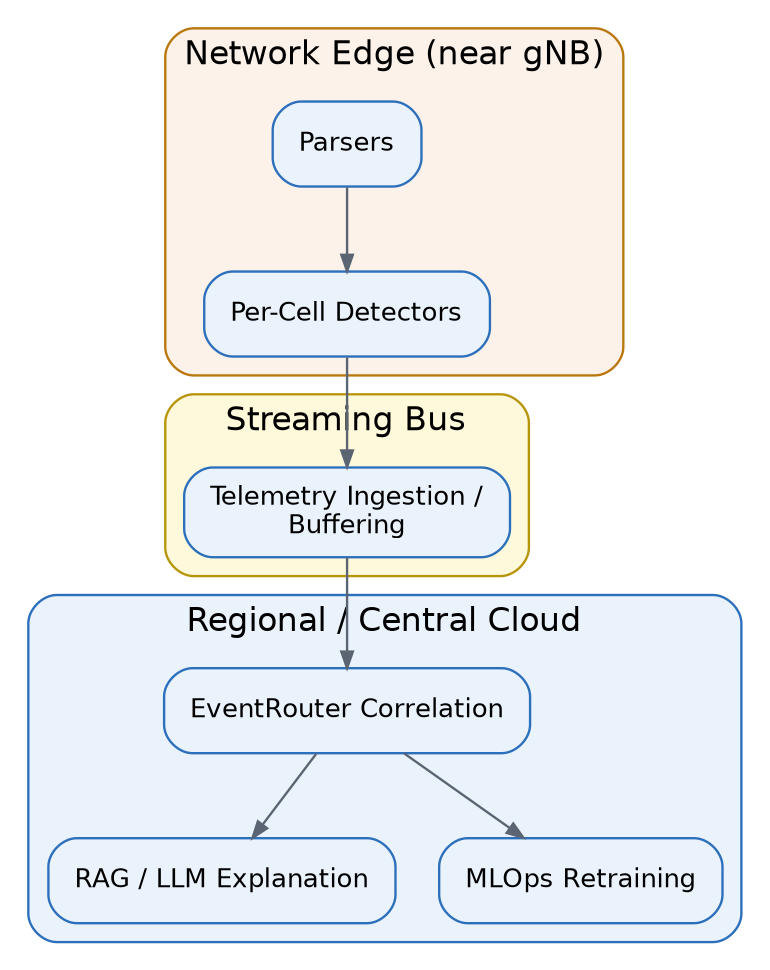
\includegraphics[width=0.85\textwidth]{figures/fig_14_3.png}
    \caption{Cloud-Native Deployment with Edge/Central Split --- Cloud-native deployment topology with latency-sensitive detection at the network edge and heavier RAG/LLM and retraining workloads in central/regional cloud.}
    \label{fig:14_3}
\end{figure}

% ---------------- Chapter 15 ----------------
\begin{figure}[htbp]
    \centering
    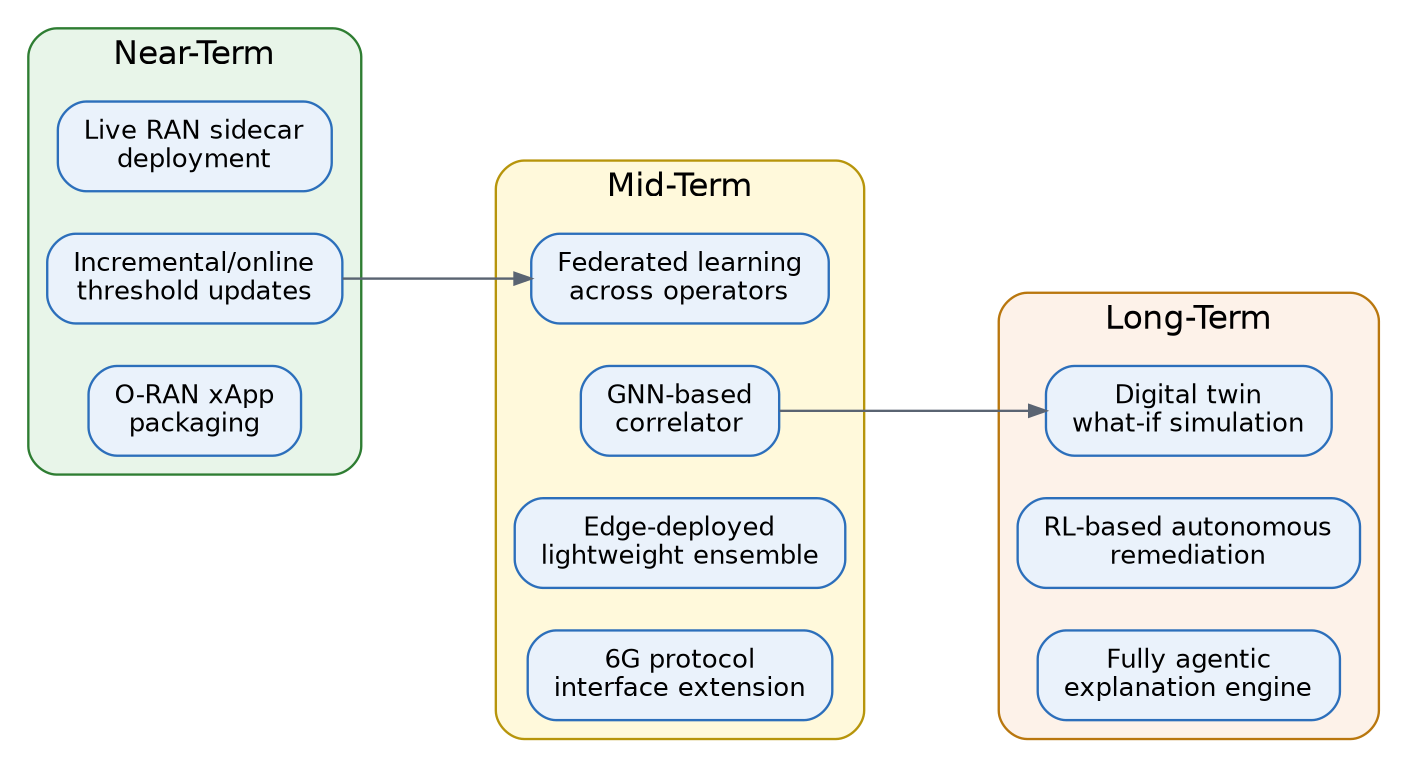
\includegraphics[width=0.85\textwidth]{figures/fig_15_1.png}
    \caption{Future Work Roadmap (Near-Term to Long-Term) --- The ten future work directions grouped by implementation horizon, from near-term engineering extensions to long-term autonomous-network research.}
    \label{fig:15_1}
\end{figure}

% ---------------- Chapter A ----------------
\begin{figure}[htbp]
    \centering
    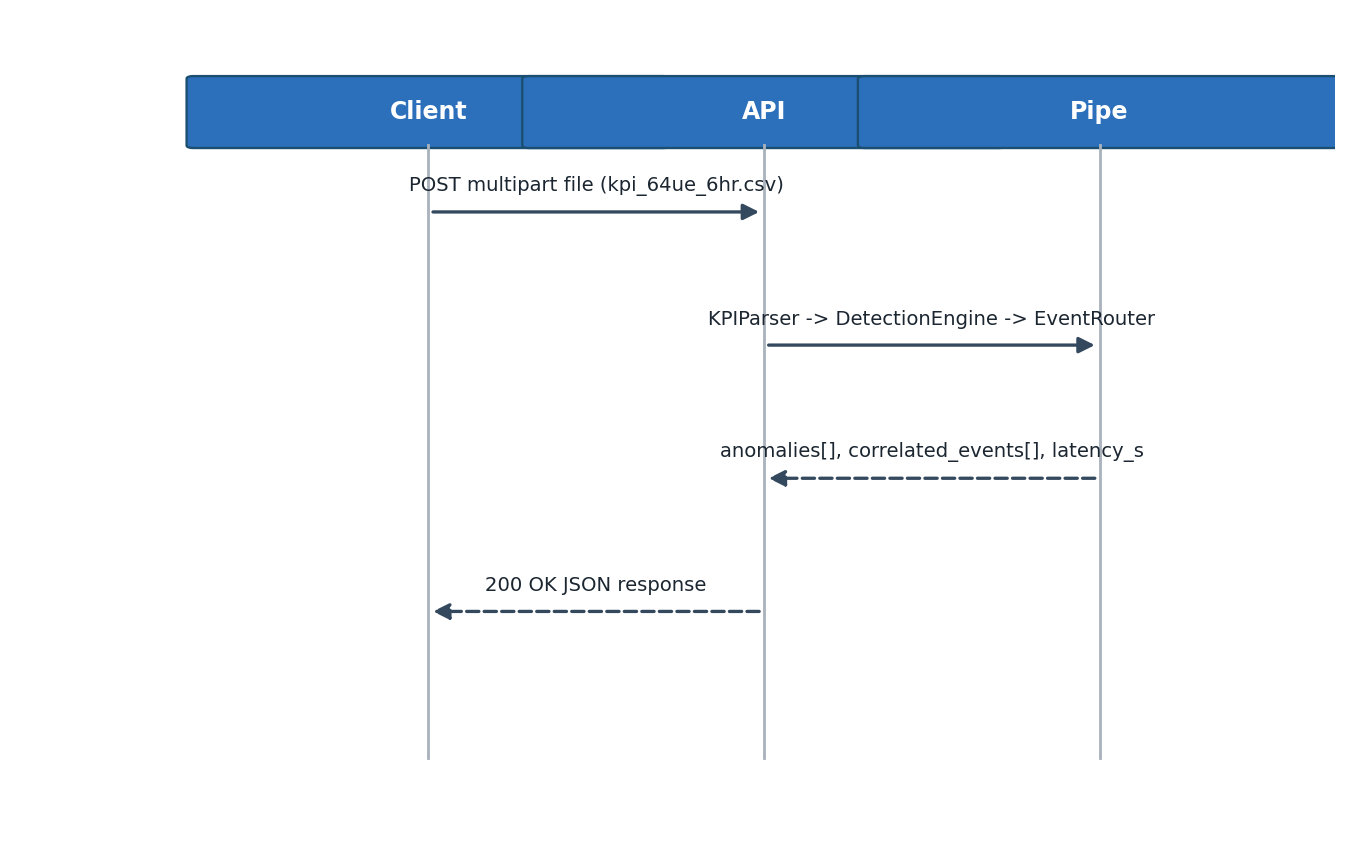
\includegraphics[width=0.85\textwidth]{figures/fig_A_1.png}
    \caption{Sample API Request/Response Flow --- Request/response sequence for the POST /analyze/kpi endpoint, from file upload through pipeline execution to JSON response.}
    \label{fig:A_1}
\end{figure}
  (place after \usepackage{graphicx})
% All images are in the figures/ subfolder - upload that folder to your Overleaf project root.
% ===================================================================

% ---------------- Chapter 1 ----------------
\begin{figure}[htbp]
    \centering
    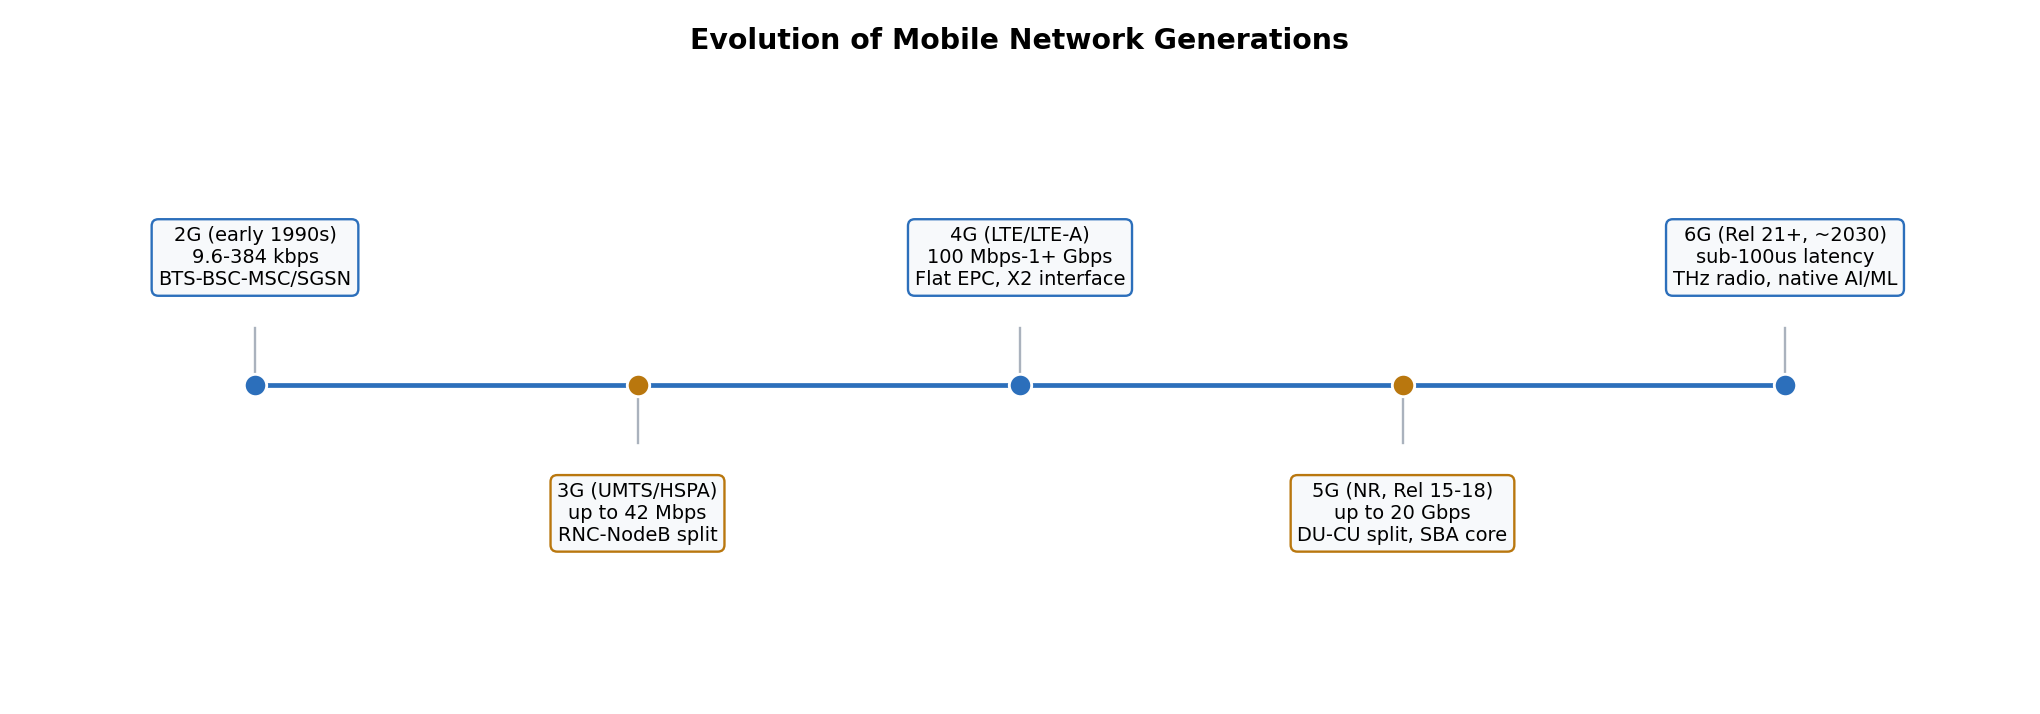
\includegraphics[width=0.85\textwidth]{figures/fig_1_1.png}
    \caption{Evolution of Mobile Network Generations --- Evolution of mobile network generations from 2G to the envisioned 6G, showing peak data rate and defining architectural change at each step.}
    \label{fig:1_1}
\end{figure}

\begin{figure}[htbp]
    \centering
    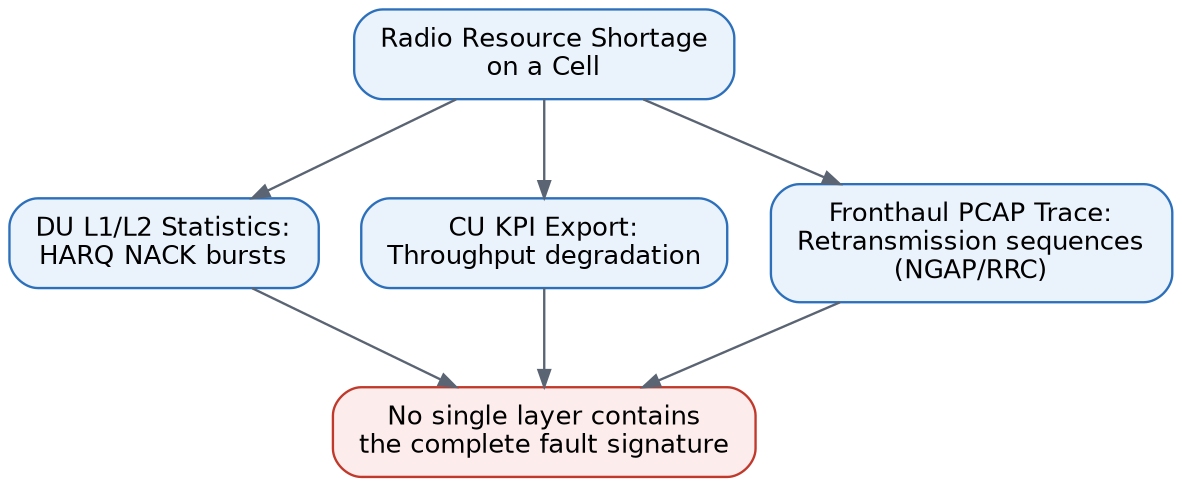
\includegraphics[width=0.85\textwidth]{figures/fig_1_2.png}
    \caption{Multi-Layer Fault Signature Propagation --- A single radio-resource fault propagates distinct, incomplete signatures into each of the three telemetry domains, motivating multi-modal detection.}
    \label{fig:1_2}
\end{figure}

\begin{figure}[htbp]
    \centering
    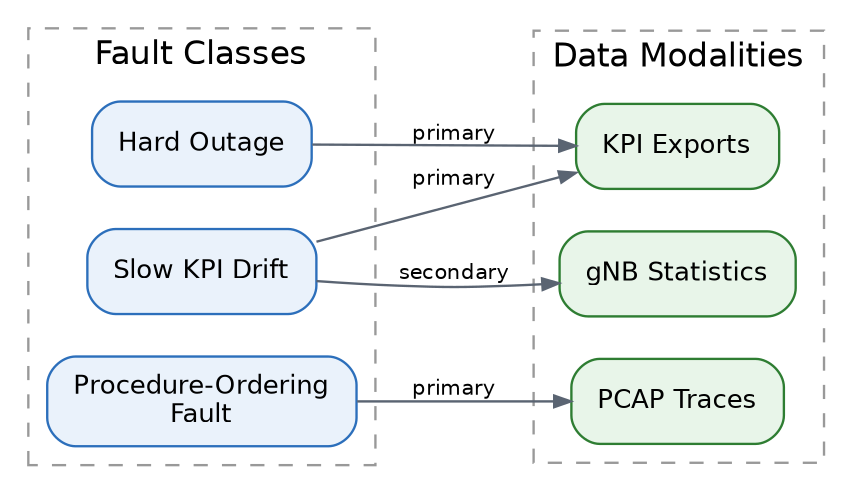
\includegraphics[width=0.85\textwidth]{figures/fig_1_3.png}
    \caption{Complementary Fault Coverage of the Three Modalities --- Mapping of the three targeted fault classes to their primary detecting modality, illustrating why no single data source covers the full fault taxonomy.}
    \label{fig:1_3}
\end{figure}

% ---------------- Chapter 2 ----------------
\begin{figure}[htbp]
    \centering
    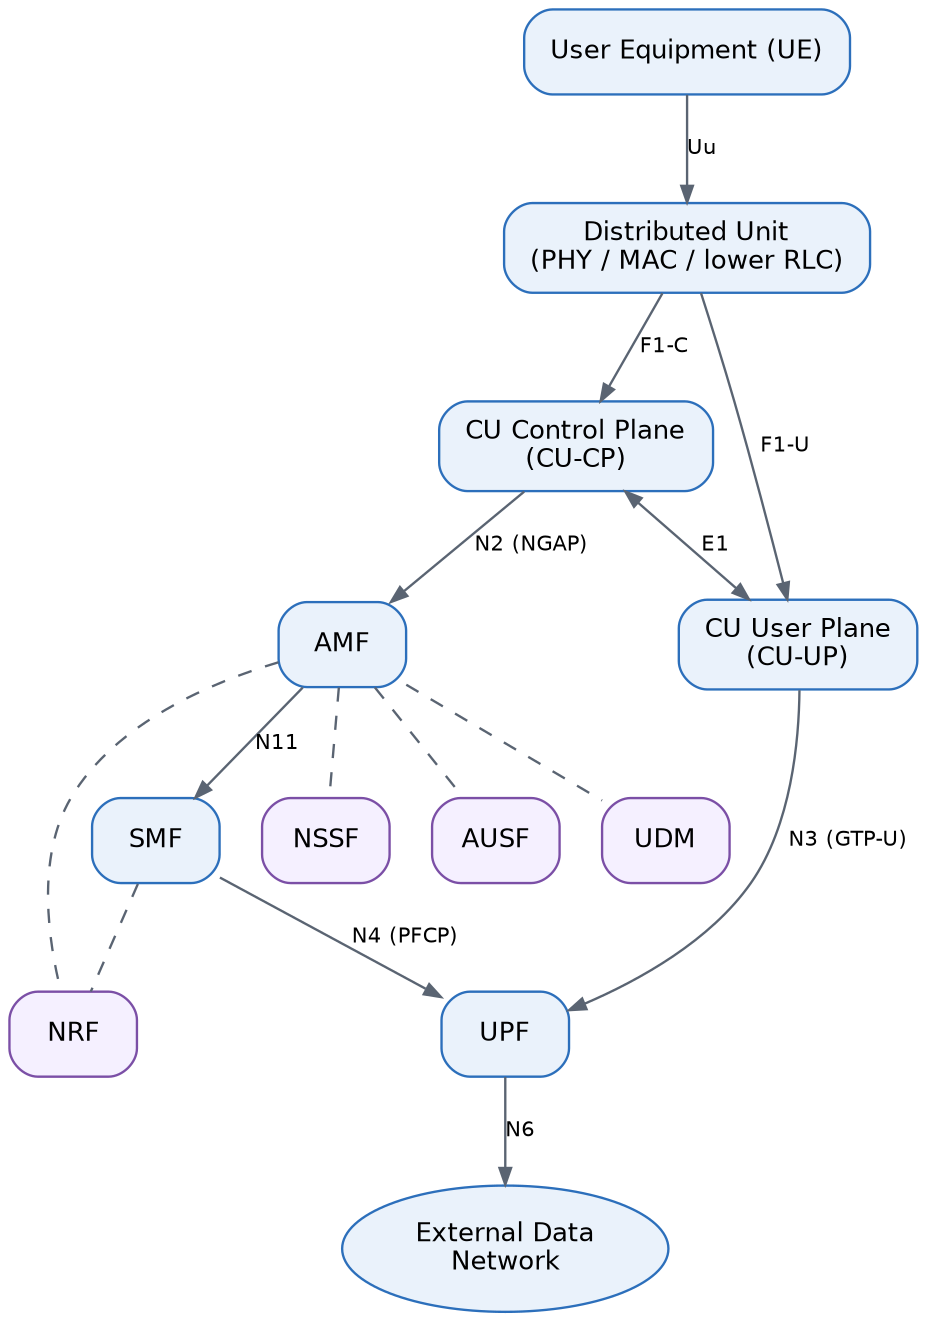
\includegraphics[width=0.85\textwidth]{figures/fig_2_1.png}
    \caption{5G Network Architecture (NG-RAN + 5GC) --- 5G system architecture showing the disaggregated NG-RAN (DU/CU-CP/CU-UP) and the Service-Based Architecture of the 5G Core.}
    \label{fig:2_1}
\end{figure}

\begin{figure}[htbp]
    \centering
    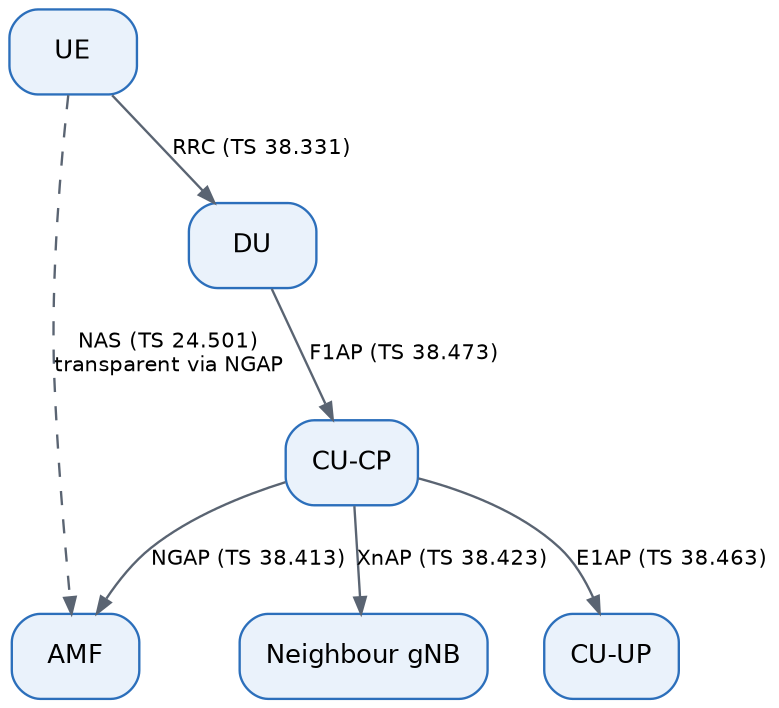
\includegraphics[width=0.85\textwidth]{figures/fig_2_2.png}
    \caption{Six Protocol Interfaces Mapped to Network Nodes --- The six 5G-NR protocol interfaces parsed by the PCAP Parser, mapped to their governing 3GPP specification and network-node endpoints.}
    \label{fig:2_2}
\end{figure}

% ---------------- Chapter 3 ----------------
\begin{figure}[htbp]
    \centering
    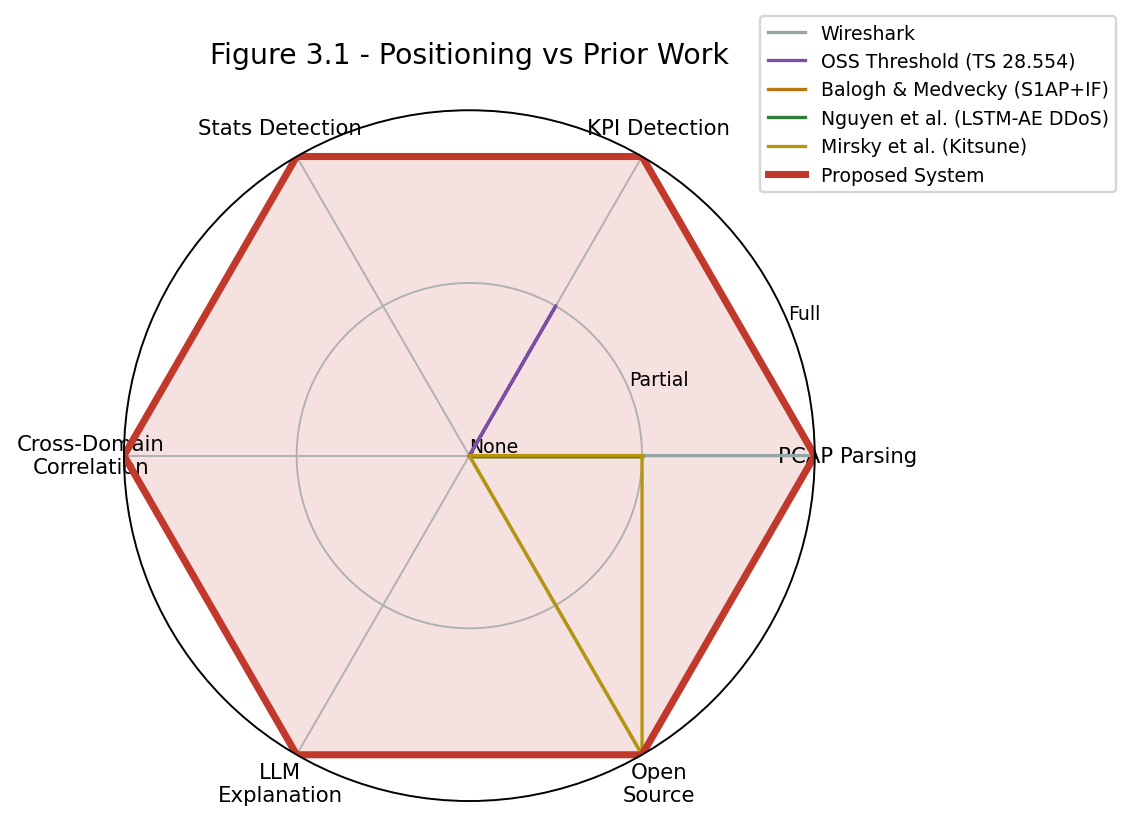
\includegraphics[width=0.85\textwidth]{figures/fig_3_1.png}
    \caption{Positioning Comparison vs. Prior Work --- Radar comparison of the proposed system against five representative prior systems across the five positioning axes of Table 3.1.}
    \label{fig:3_1}
\end{figure}

% ---------------- Chapter 4 ----------------
\begin{figure}[htbp]
    \centering
    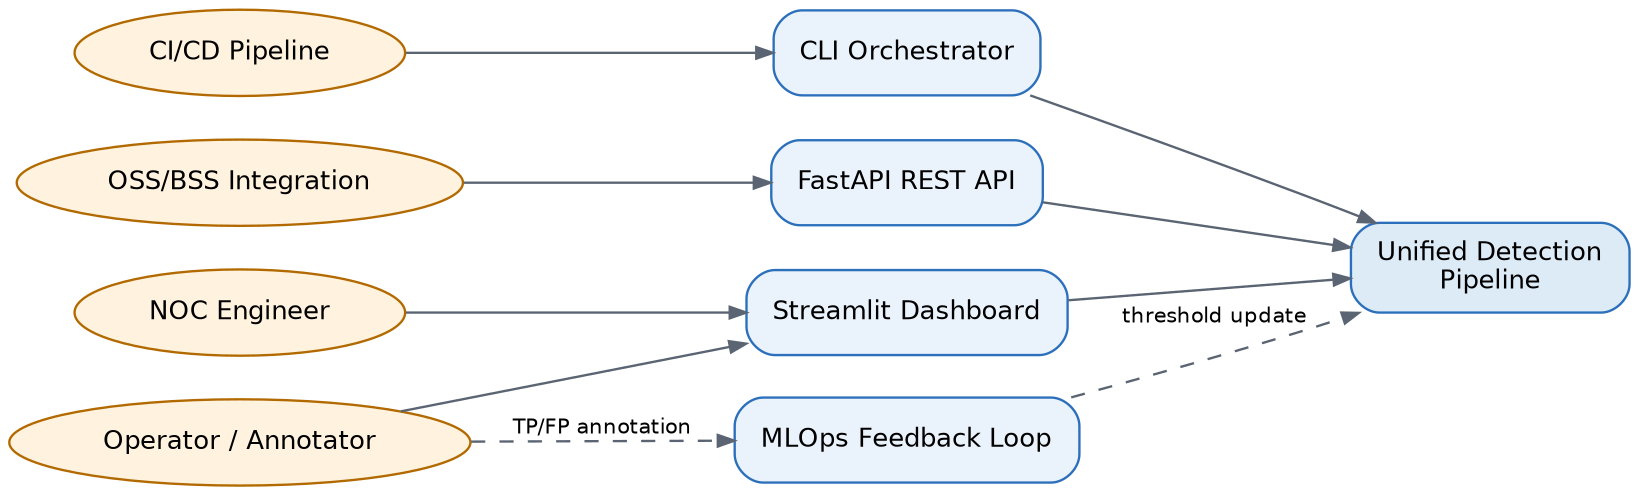
\includegraphics[width=0.85\textwidth]{figures/fig_4_1.png}
    \caption{Use Case Diagram --- Actors and access interfaces for the Unified Telecom Analyzer, tracing each functional requirement to its consuming role.}
    \label{fig:4_1}
\end{figure}

% ---------------- Chapter 5 ----------------
\begin{figure}[htbp]
    \centering
    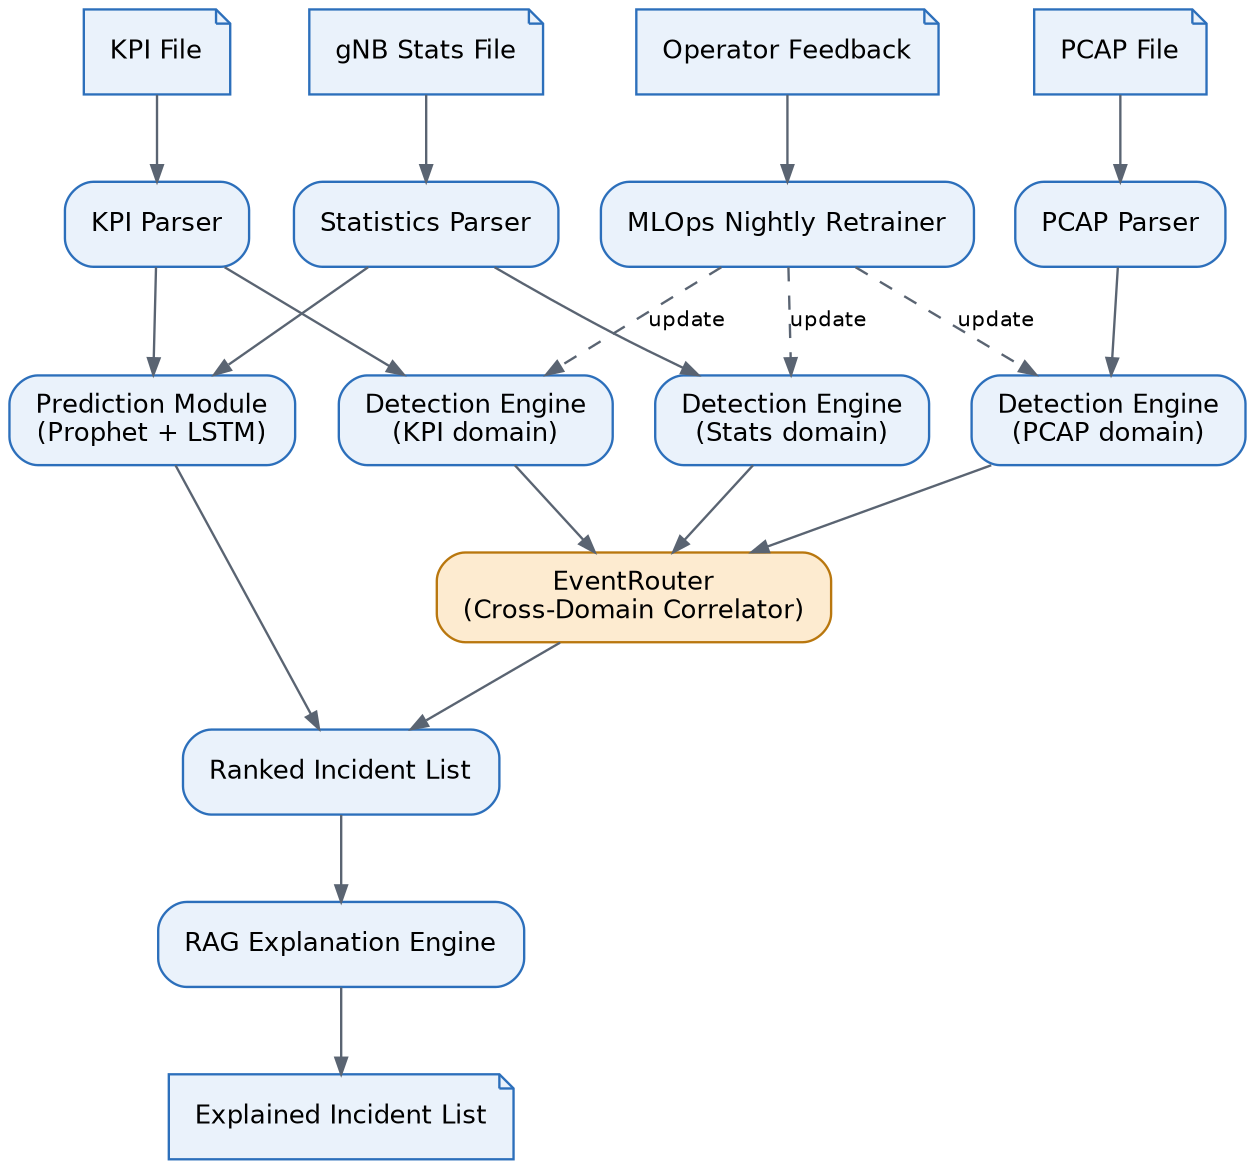
\includegraphics[width=0.85\textwidth]{figures/fig_5_1.png}
    \caption{Unified Pipeline End-to-End Control Flow --- End-to-end control flow of the Unified Telecom Analyzer, showing the Parse to Detect to Correlate to Explain pipeline with parallel Prediction and MLOps feedback branches.}
    \label{fig:5_1}
\end{figure}

\begin{figure}[htbp]
    \centering
    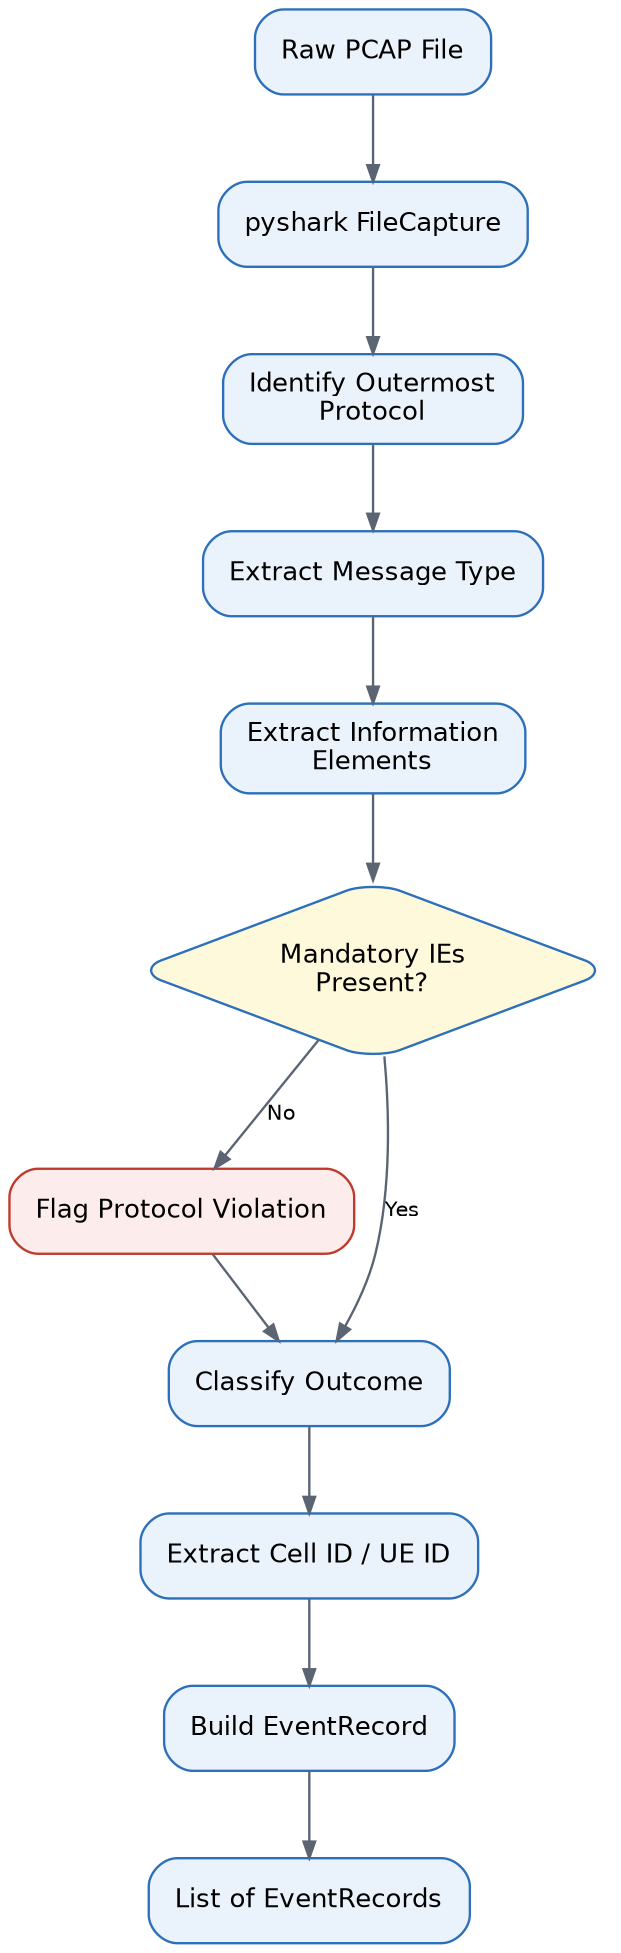
\includegraphics[width=0.85\textwidth]{figures/fig_5_2.png}
    \caption{PCAP Parser Workflow --- PCAP Parser processing workflow, including the spec-alignment branch that flags protocol violations independently of the anomaly ensemble.}
    \label{fig:5_2}
\end{figure}

\begin{figure}[htbp]
    \centering
    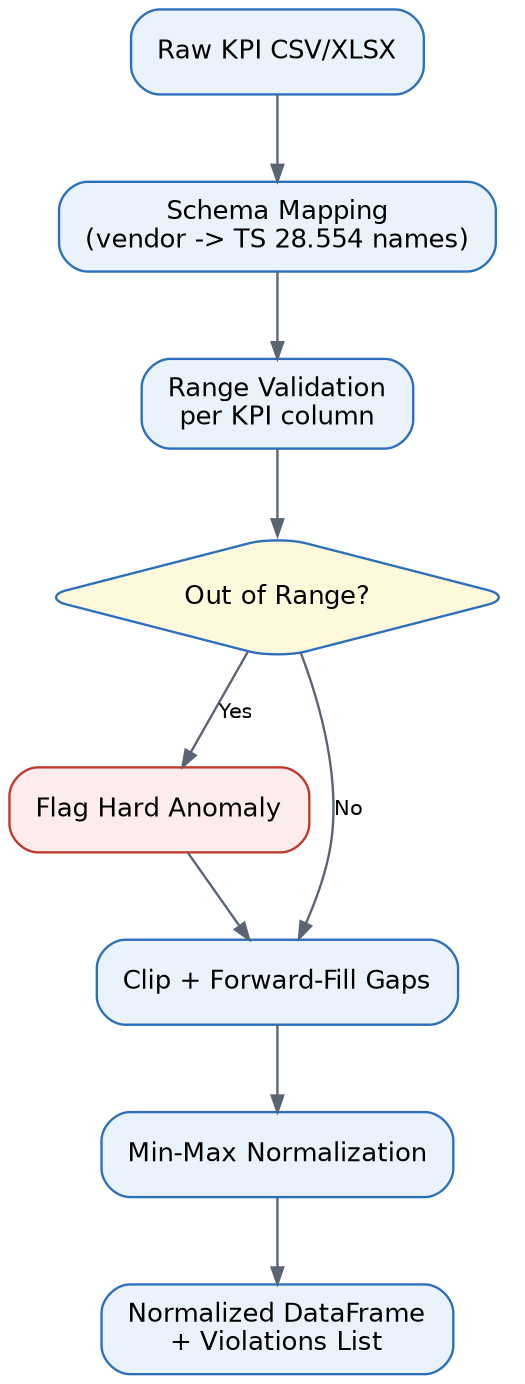
\includegraphics[width=0.85\textwidth]{figures/fig_5_3.png}
    \caption{KPI Parser Three-Stage Pipeline --- KPI Parser three-stage processing pipeline: schema mapping, range validation, and normalization.}
    \label{fig:5_3}
\end{figure}

\begin{figure}[htbp]
    \centering
    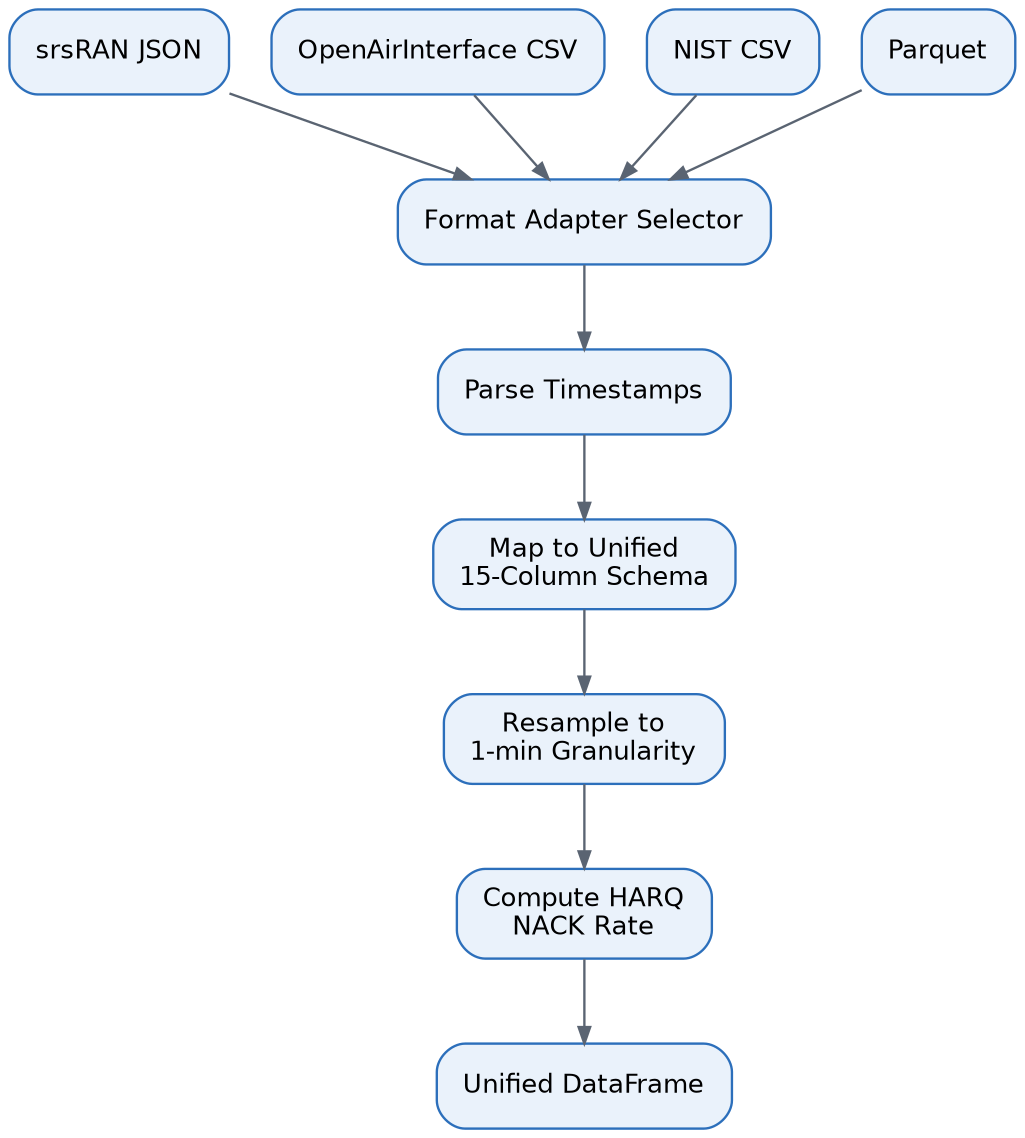
\includegraphics[width=0.85\textwidth]{figures/fig_5_4.png}
    \caption{Statistics Parser Multi-Format Adapter Architecture --- Statistics Parser adapter architecture unifying four input formats into a single 15-column schema.}
    \label{fig:5_4}
\end{figure}

\begin{figure}[htbp]
    \centering
    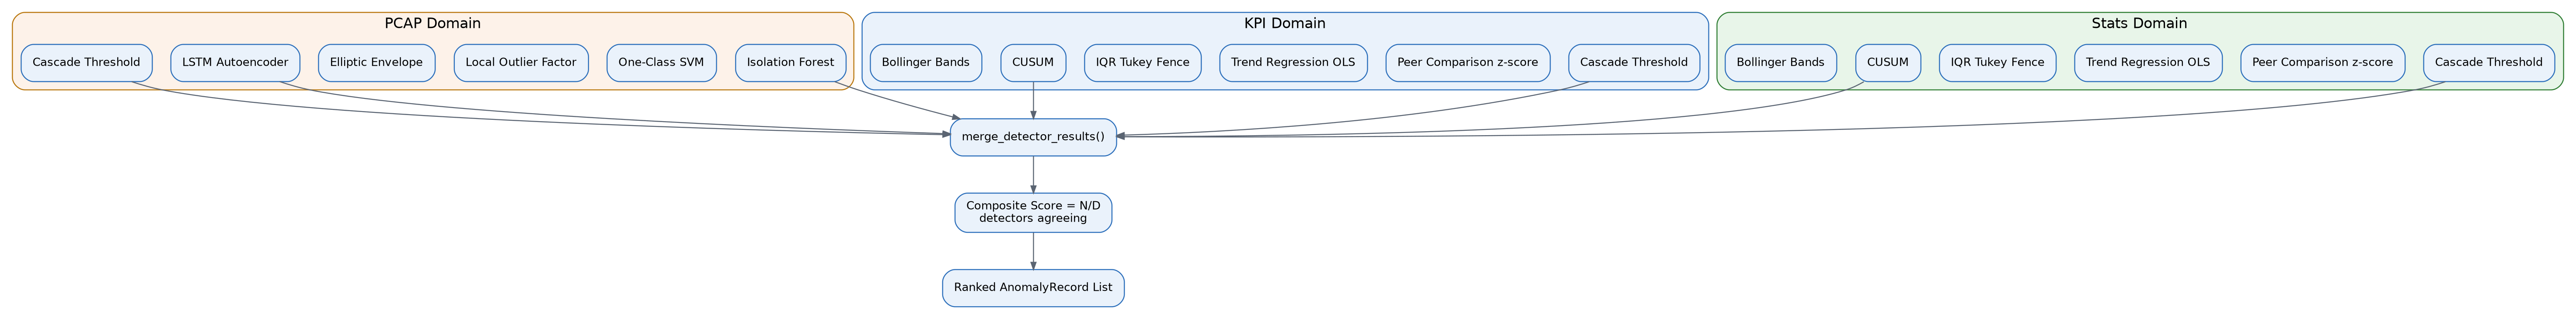
\includegraphics[width=0.85\textwidth]{figures/fig_5_5.png}
    \caption{18-Detector Ensemble Architecture --- 18-detector ensemble architecture: six algorithm families instantiated across three data domains, merged into a composite severity score.}
    \label{fig:5_5}
\end{figure}

\begin{figure}[htbp]
    \centering
    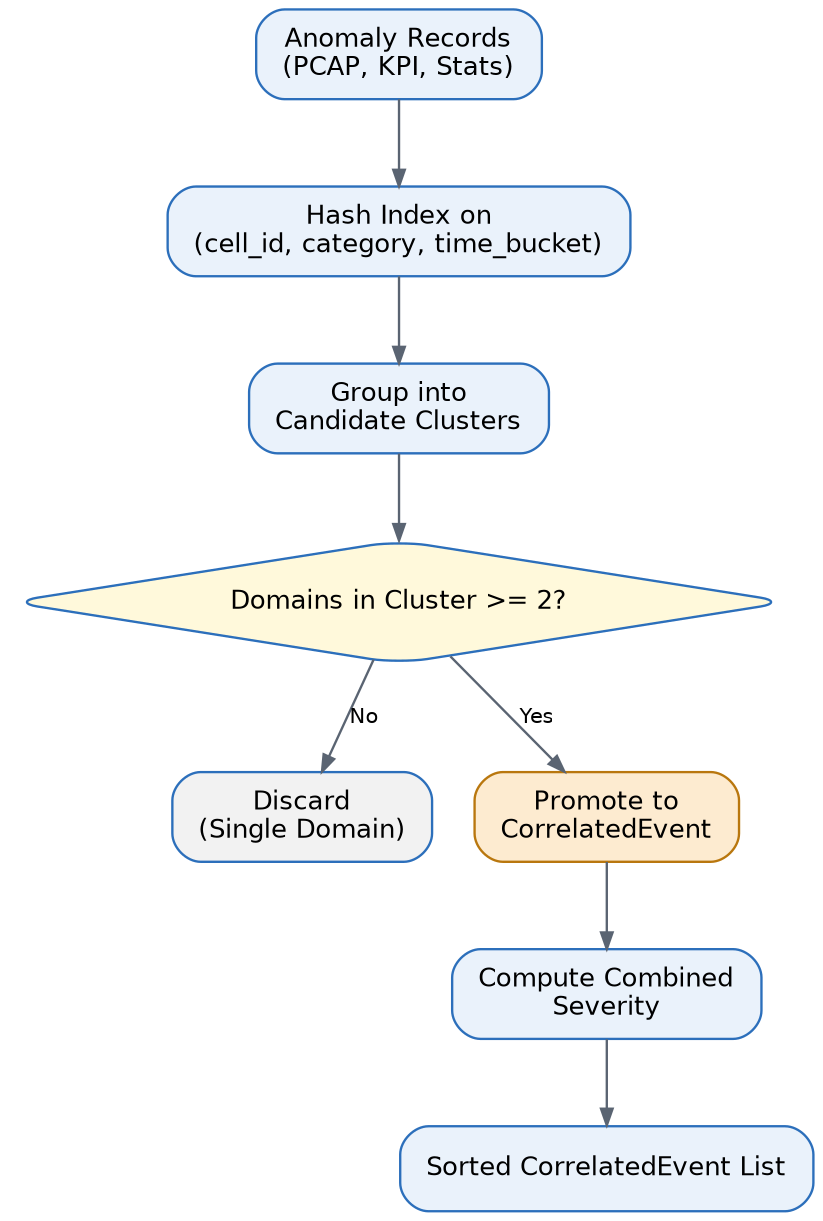
\includegraphics[width=0.85\textwidth]{figures/fig_5_6.png}
    \caption{EventRouter Cross-Domain Correlation --- EventRouter cross-domain correlation mechanism, promoting multi-domain anomaly clusters to CorrelatedEvents.}
    \label{fig:5_6}
\end{figure}

\begin{figure}[htbp]
    \centering
    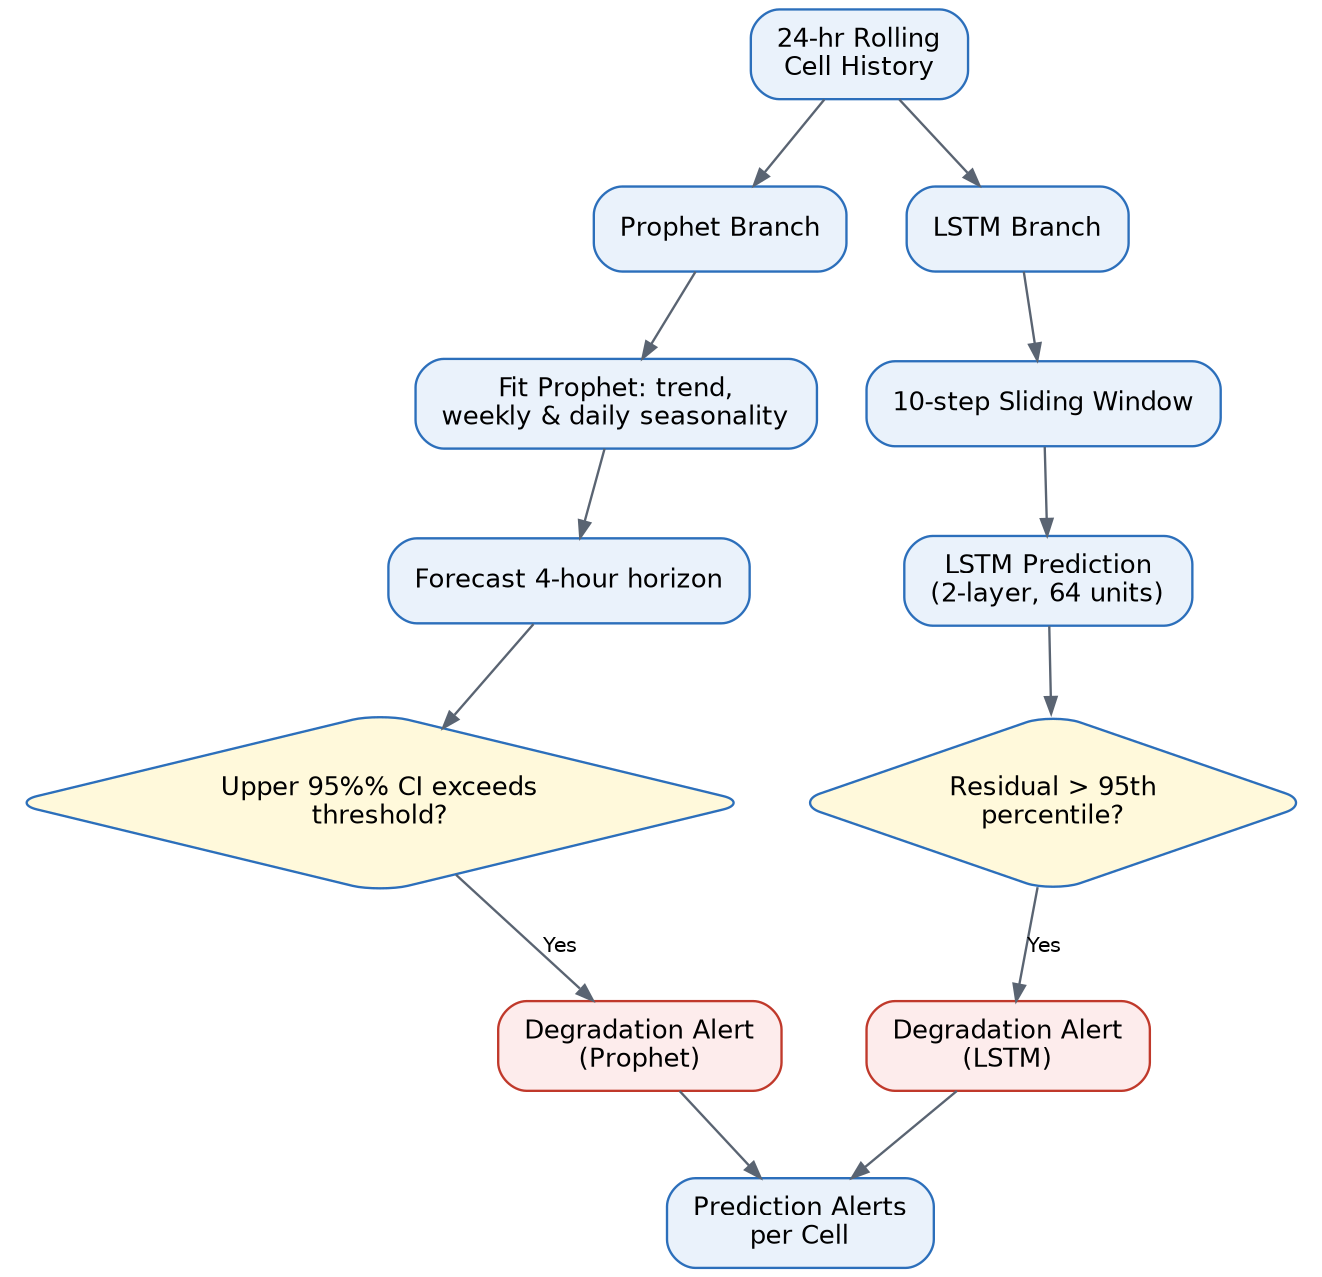
\includegraphics[width=0.85\textwidth]{figures/fig_5_7.png}
    \caption{Prediction Module Dual-Branch Design --- Dual-branch Prediction Module combining Prophet (seasonal patterns) and LSTM (non-linear sudden onset).}
    \label{fig:5_7}
\end{figure}

\begin{figure}[htbp]
    \centering
    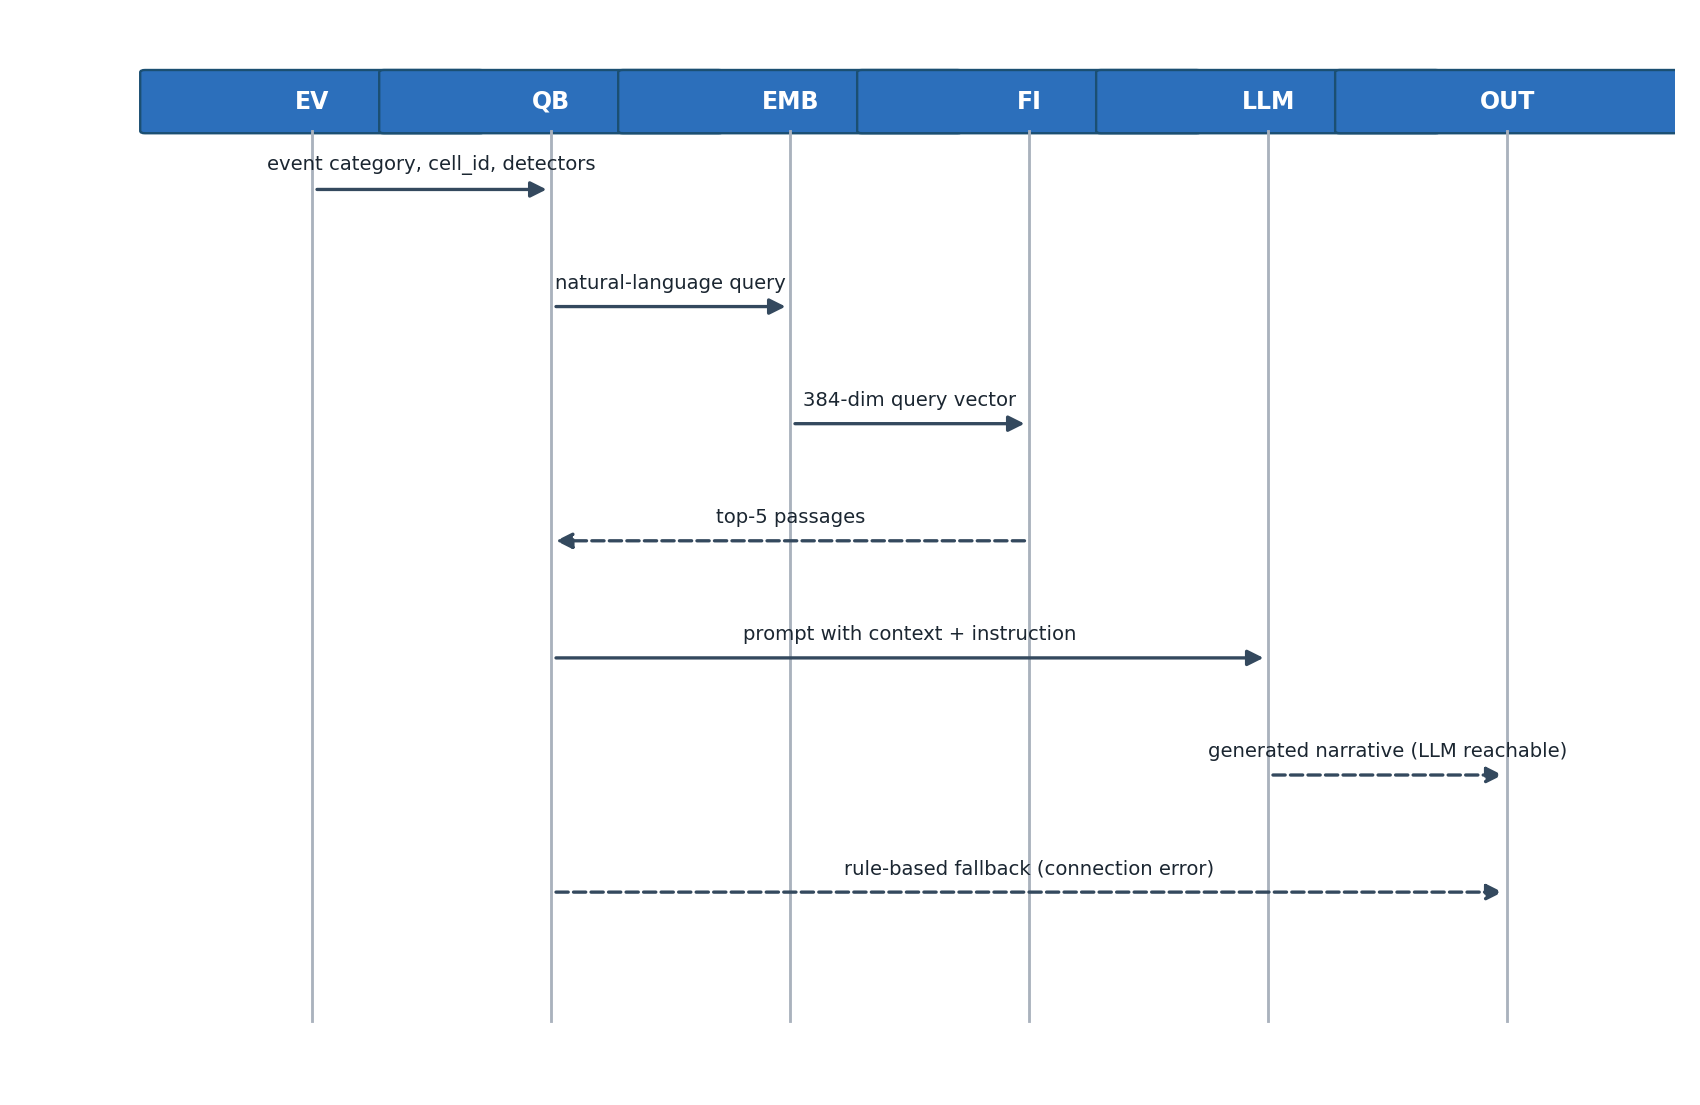
\includegraphics[width=0.85\textwidth]{figures/fig_5_8.png}
    \caption{RAG Explanation Engine Flow --- RAG Explanation Engine pipeline: query construction, FAISS retrieval, and LLM generation with offline fallback.}
    \label{fig:5_8}
\end{figure}

\begin{figure}[htbp]
    \centering
    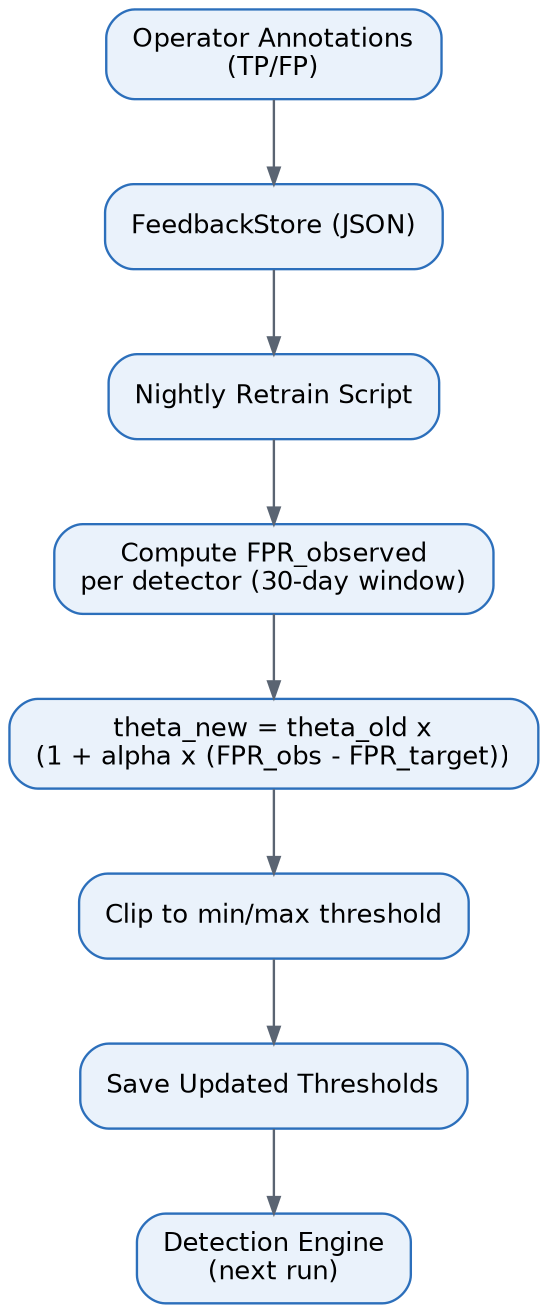
\includegraphics[width=0.85\textwidth]{figures/fig_5_9.png}
    \caption{MLOps Nightly Feedback Loop --- MLOps nightly feedback loop adjusting per-detector thresholds from operator false-positive annotations.}
    \label{fig:5_9}
\end{figure}

\begin{figure}[htbp]
    \centering
    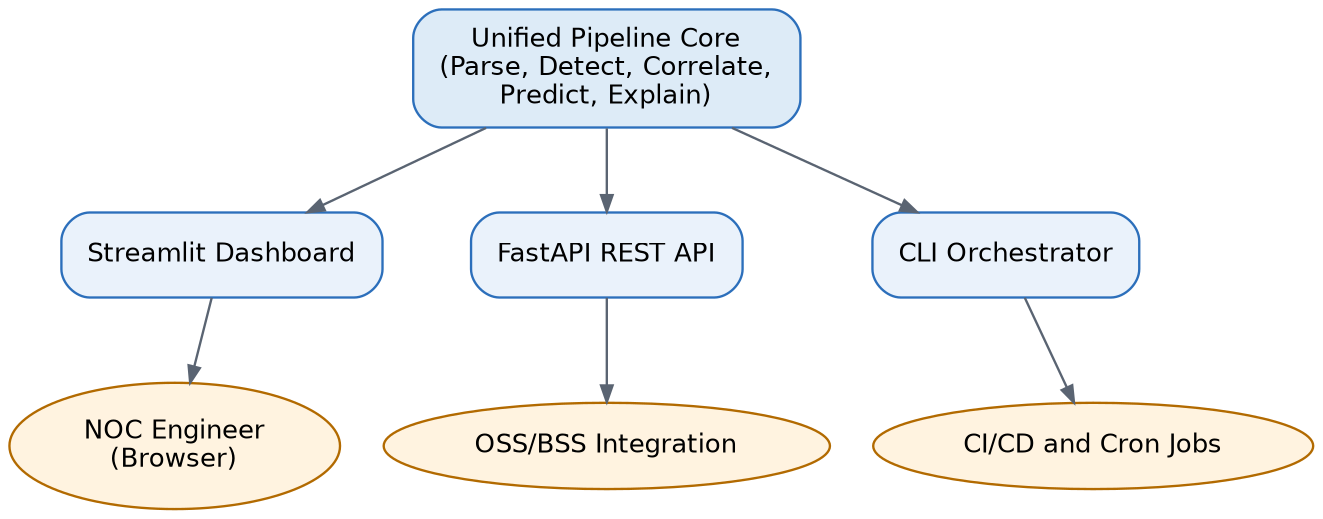
\includegraphics[width=0.85\textwidth]{figures/fig_5_10.png}
    \caption{Three Access Interfaces --- Three access interfaces (Dashboard, REST API, CLI) built on a shared pipeline core.}
    \label{fig:5_10}
\end{figure}

\begin{figure}[htbp]
    \centering
    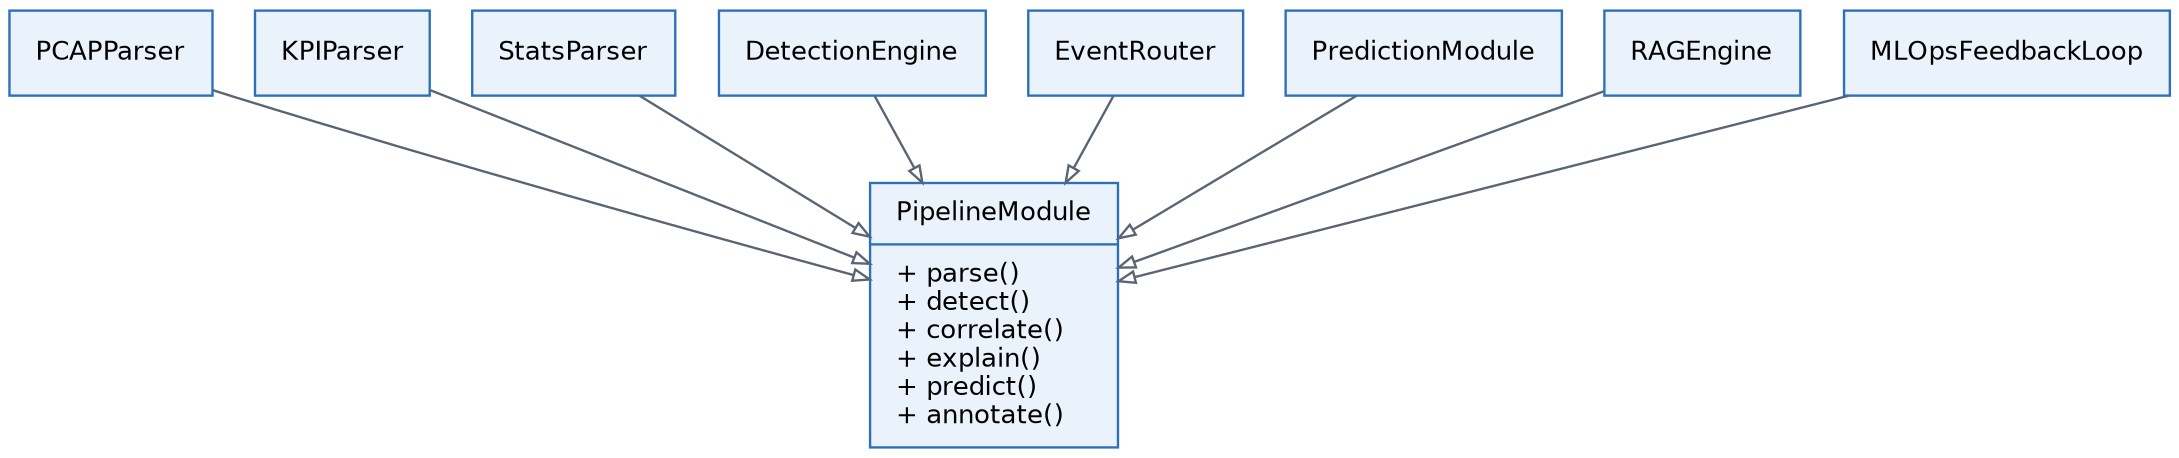
\includegraphics[width=0.85\textwidth]{figures/fig_5_11.png}
    \caption{Common Module Interface (Separation of Concerns) --- Common module interface enabling independent testing and future substitution of any pipeline component.}
    \label{fig:5_11}
\end{figure}

% ---------------- Chapter 6 ----------------
\begin{figure}[htbp]
    \centering
    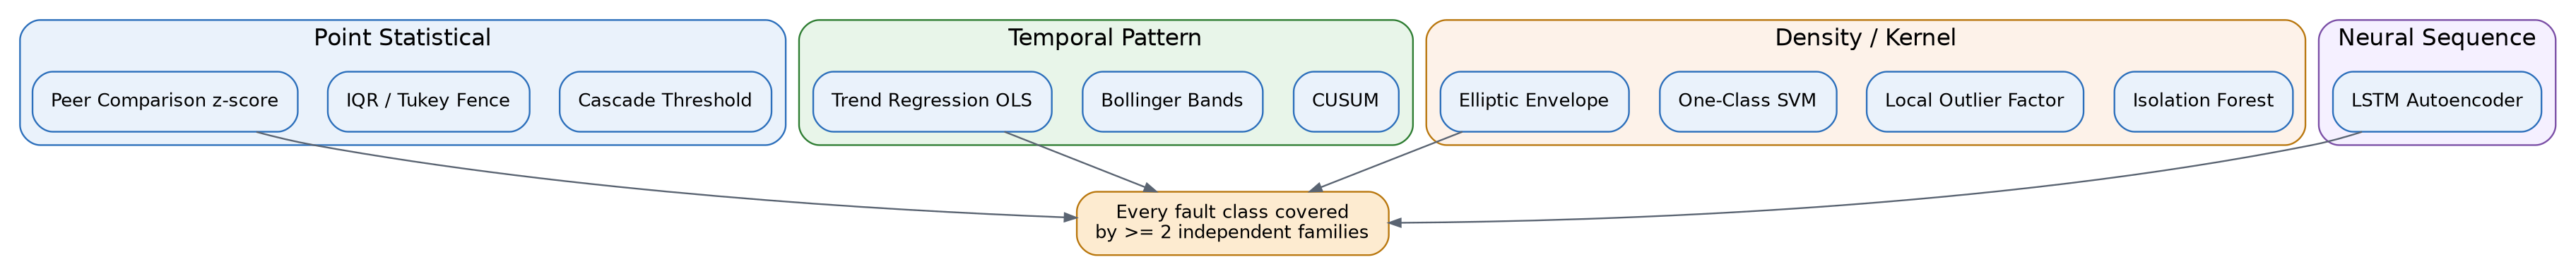
\includegraphics[width=0.85\textwidth]{figures/fig_6_1.png}
    \caption{Detector Family Taxonomy (Ensemble Coverage Principle) --- The twelve detection algorithms partitioned into four orthogonal families, the theoretical basis for the ensemble's fault-class coverage.}
    \label{fig:6_1}
\end{figure}

% ---------------- Chapter 7 ----------------
\begin{figure}[htbp]
    \centering
    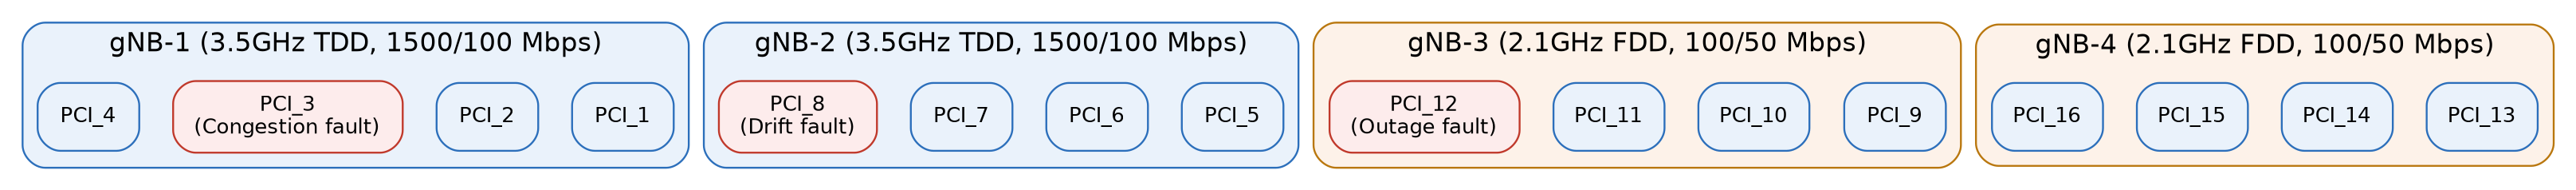
\includegraphics[width=0.85\textwidth]{figures/fig_7_1.png}
    \caption{Evaluation Network Topology --- Evaluation testbed topology: 4 gNBs / 16 cells / 64 UEs, with the three fault-injection cells highlighted.}
    \label{fig:7_1}
\end{figure}

\begin{figure}[htbp]
    \centering
    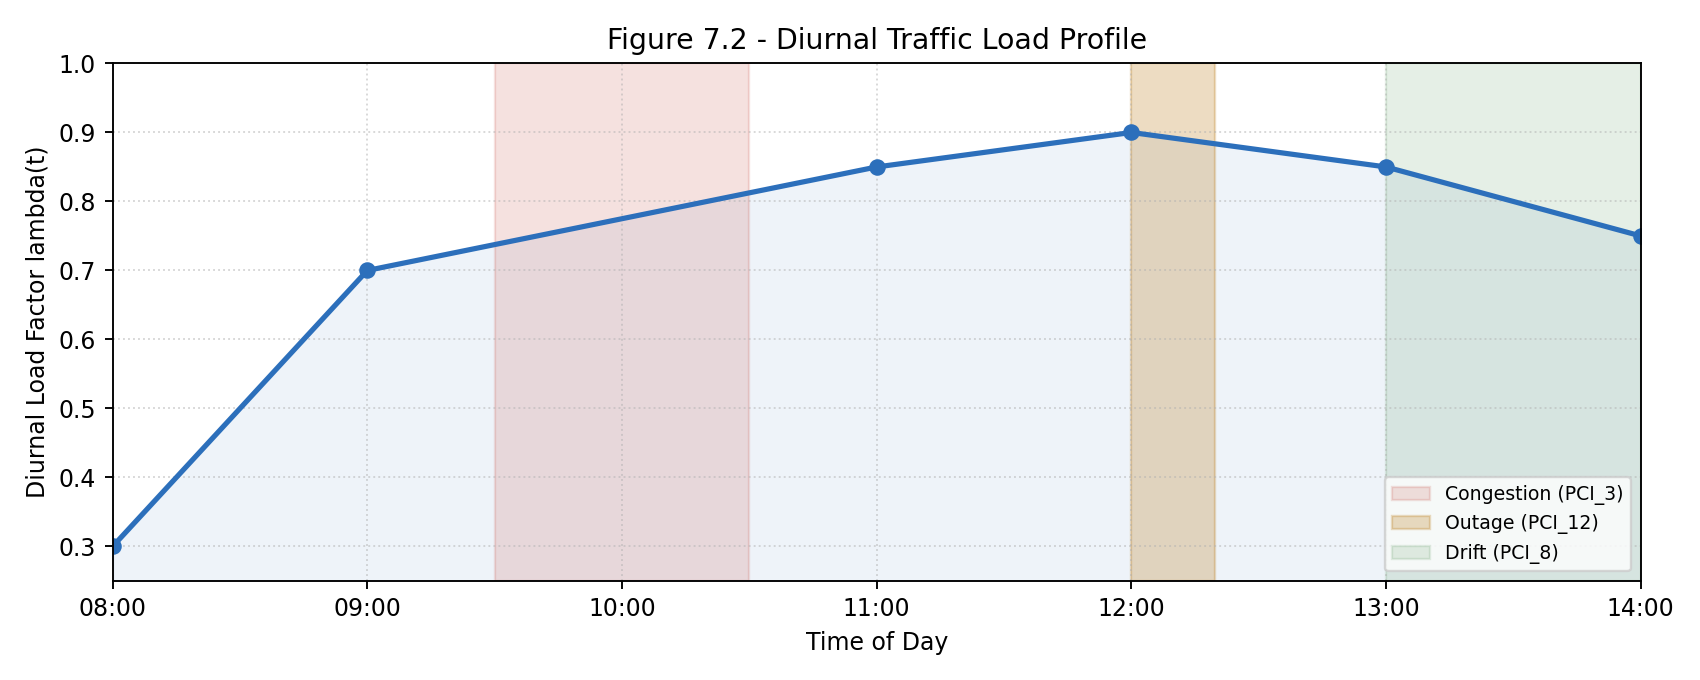
\includegraphics[width=0.85\textwidth]{figures/fig_7_2.png}
    \caption{Diurnal Traffic Load Profile --- Diurnal load factor over the 6-hour simulation window, with the three fault-injection windows marked.}
    \label{fig:7_2}
\end{figure}

\begin{figure}[htbp]
    \centering
    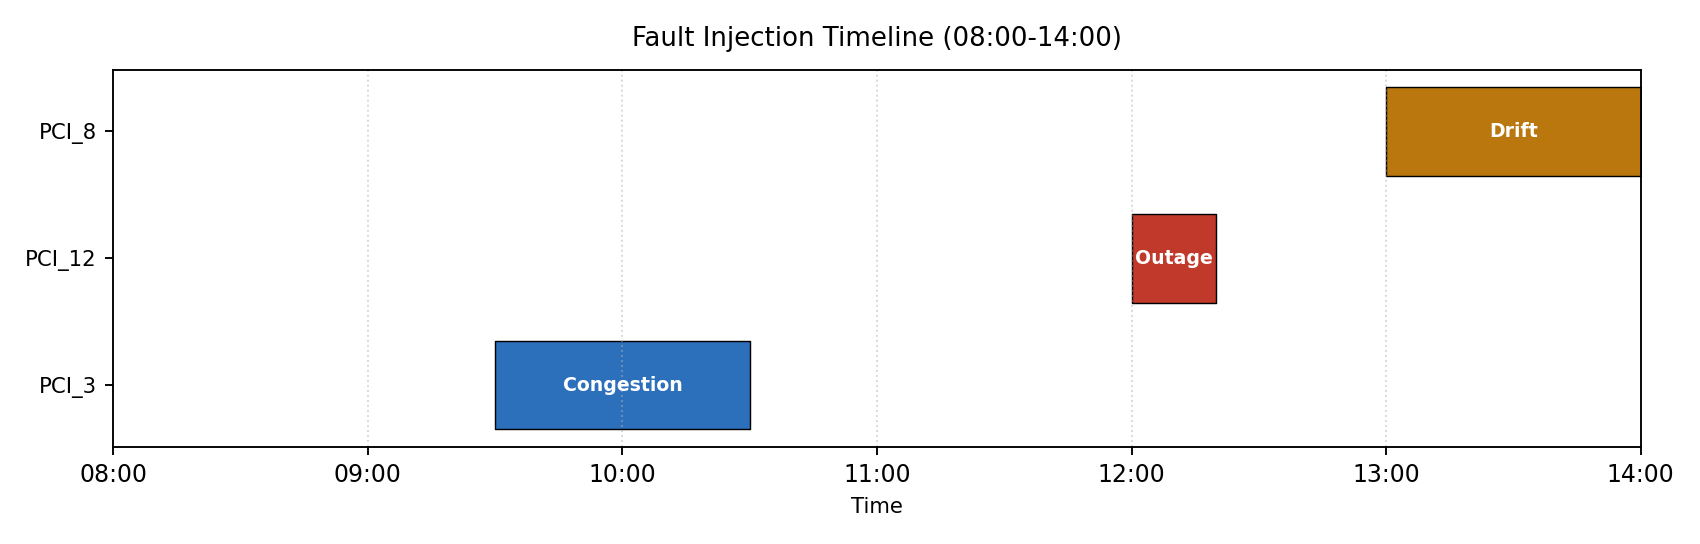
\includegraphics[width=0.85\textwidth]{figures/fig_7_3.png}
    \caption{Fault Injection Timeline --- Timeline of the three concurrent injected fault scenarios across the 6-hour evaluation window.}
    \label{fig:7_3}
\end{figure}

\begin{figure}[htbp]
    \centering
    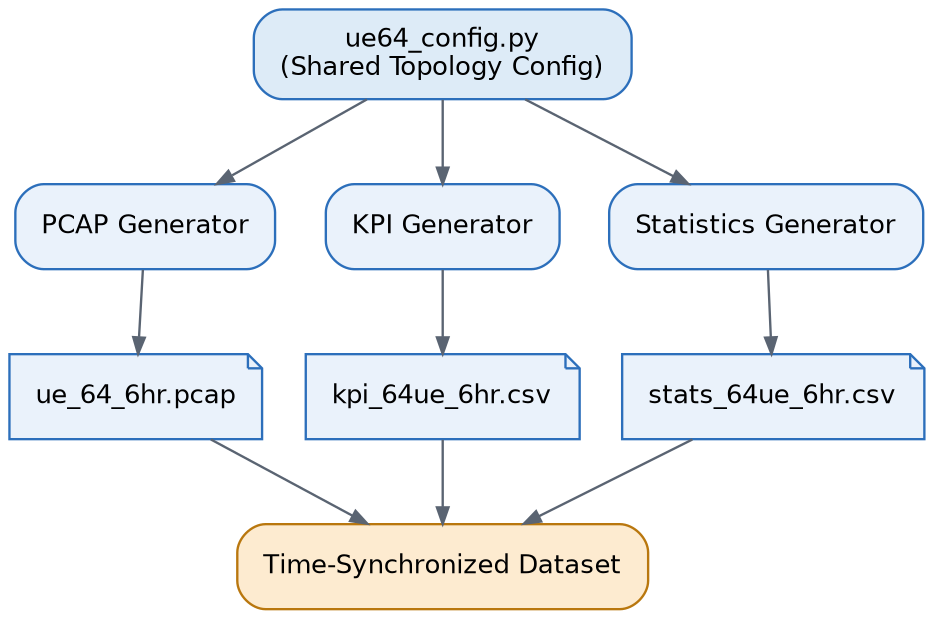
\includegraphics[width=0.85\textwidth]{figures/fig_7_4.png}
    \caption{Dataset Generation Pipeline --- Synthetic dataset generation pipeline: a single shared topology configuration produces three time-synchronized, cross-domain-consistent data files.}
    \label{fig:7_4}
\end{figure}

% ---------------- Chapter 8 ----------------
\begin{figure}[htbp]
    \centering
    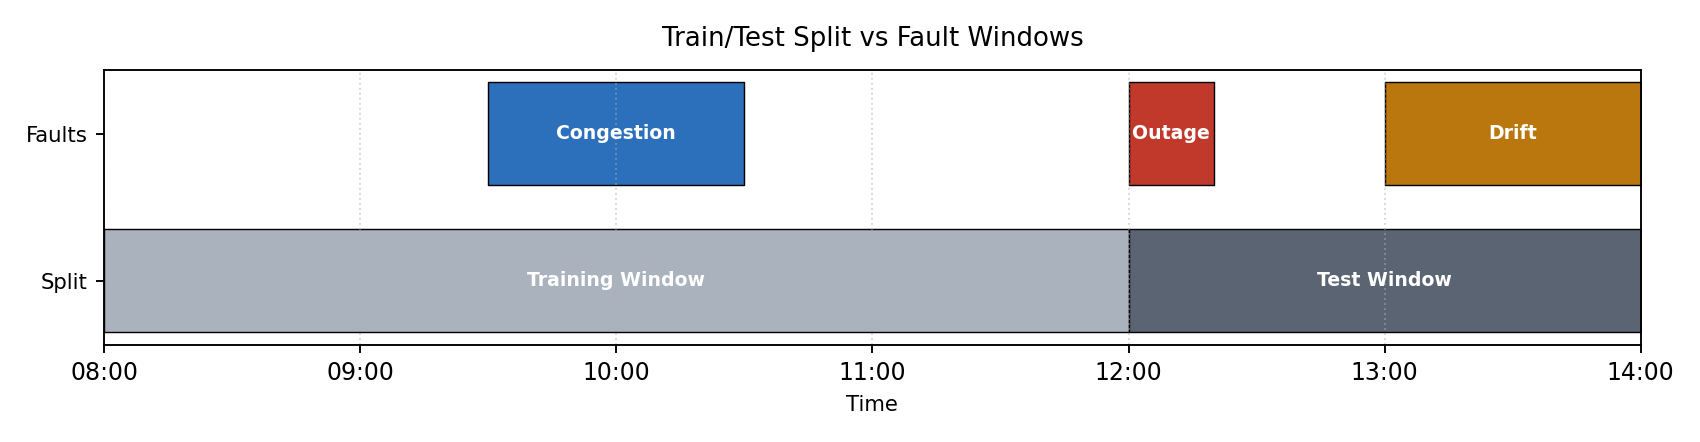
\includegraphics[width=0.85\textwidth]{figures/fig_8_1.png}
    \caption{Train/Test Temporal Split with Fault Overlay --- Temporal train/test split overlaid with the three fault windows, showing that the congestion fault straddles both windows while outage and drift fall entirely in the test window.}
    \label{fig:8_1}
\end{figure}

% ---------------- Chapter 9 ----------------
\begin{figure}[htbp]
    \centering
    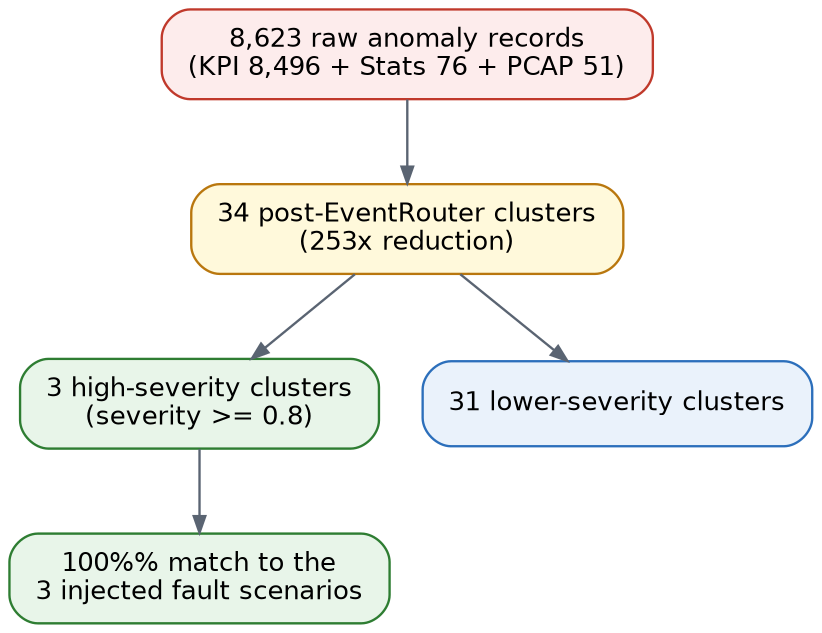
\includegraphics[width=0.85\textwidth]{figures/fig_9_1.png}
    \caption{EventRouter Alarm-Volume Reduction Funnel --- Alarm-volume reduction achieved by the EventRouter: 8,623 raw records collapse to 34 operator-visible clusters, with all three high-severity clusters correctly matching the injected faults.}
    \label{fig:9_1}
\end{figure}

\begin{figure}[htbp]
    \centering
    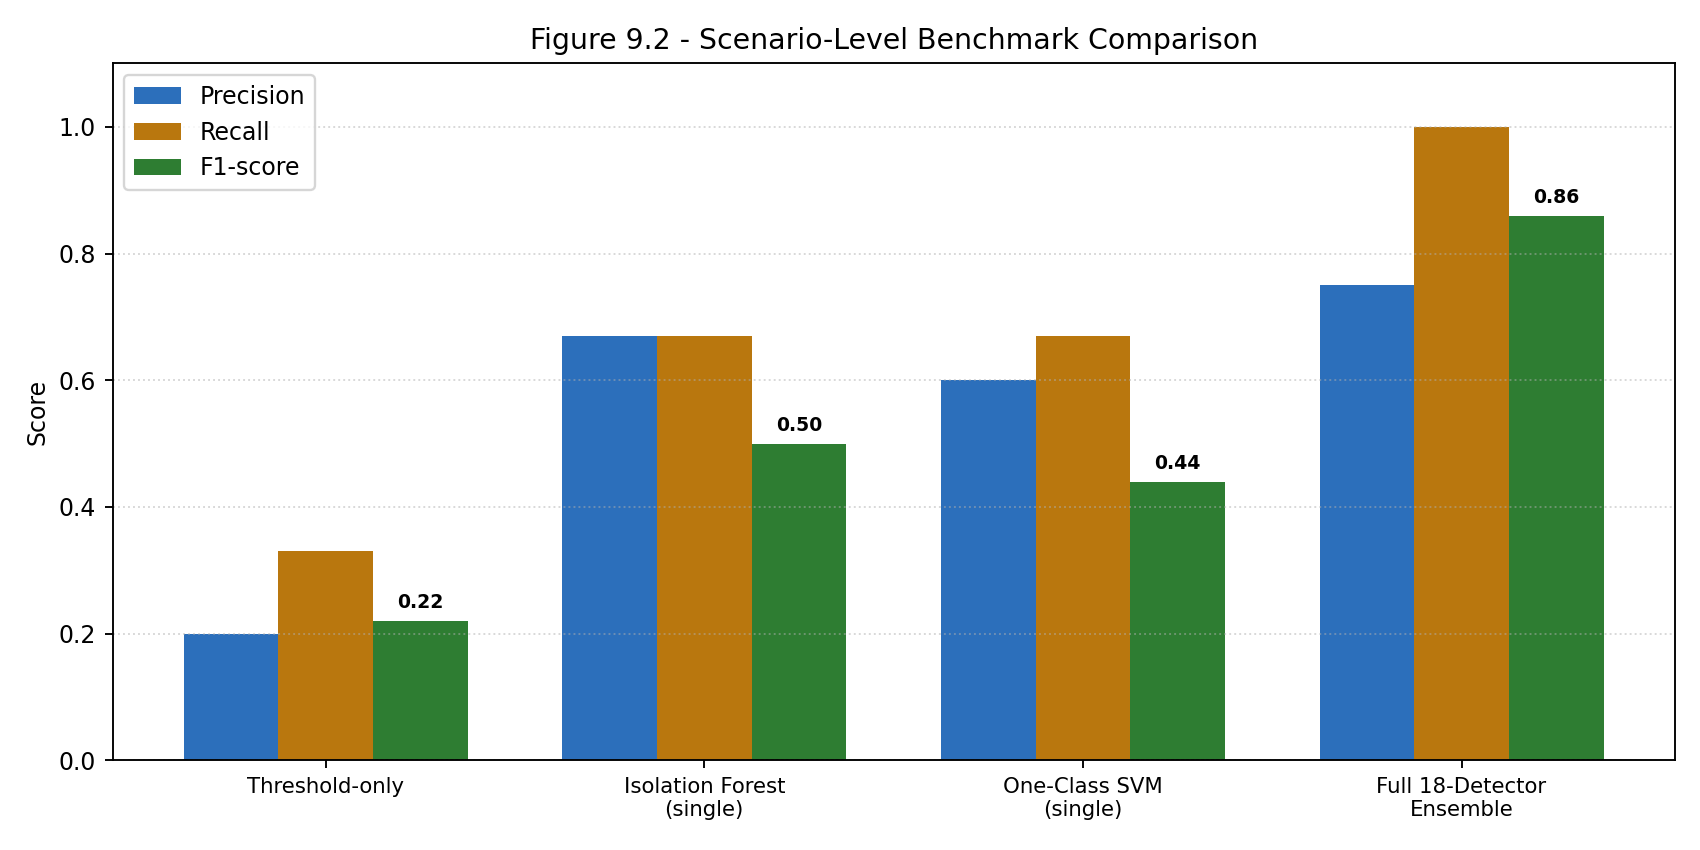
\includegraphics[width=0.85\textwidth]{figures/fig_9_2.png}
    \caption{Benchmark Comparison (Precision/Recall/F1) --- Scenario-level Precision, Recall, and F1 across the threshold-only baseline, two single-detector baselines, and the full 18-detector ensemble.}
    \label{fig:9_2}
\end{figure}

\begin{figure}[htbp]
    \centering
    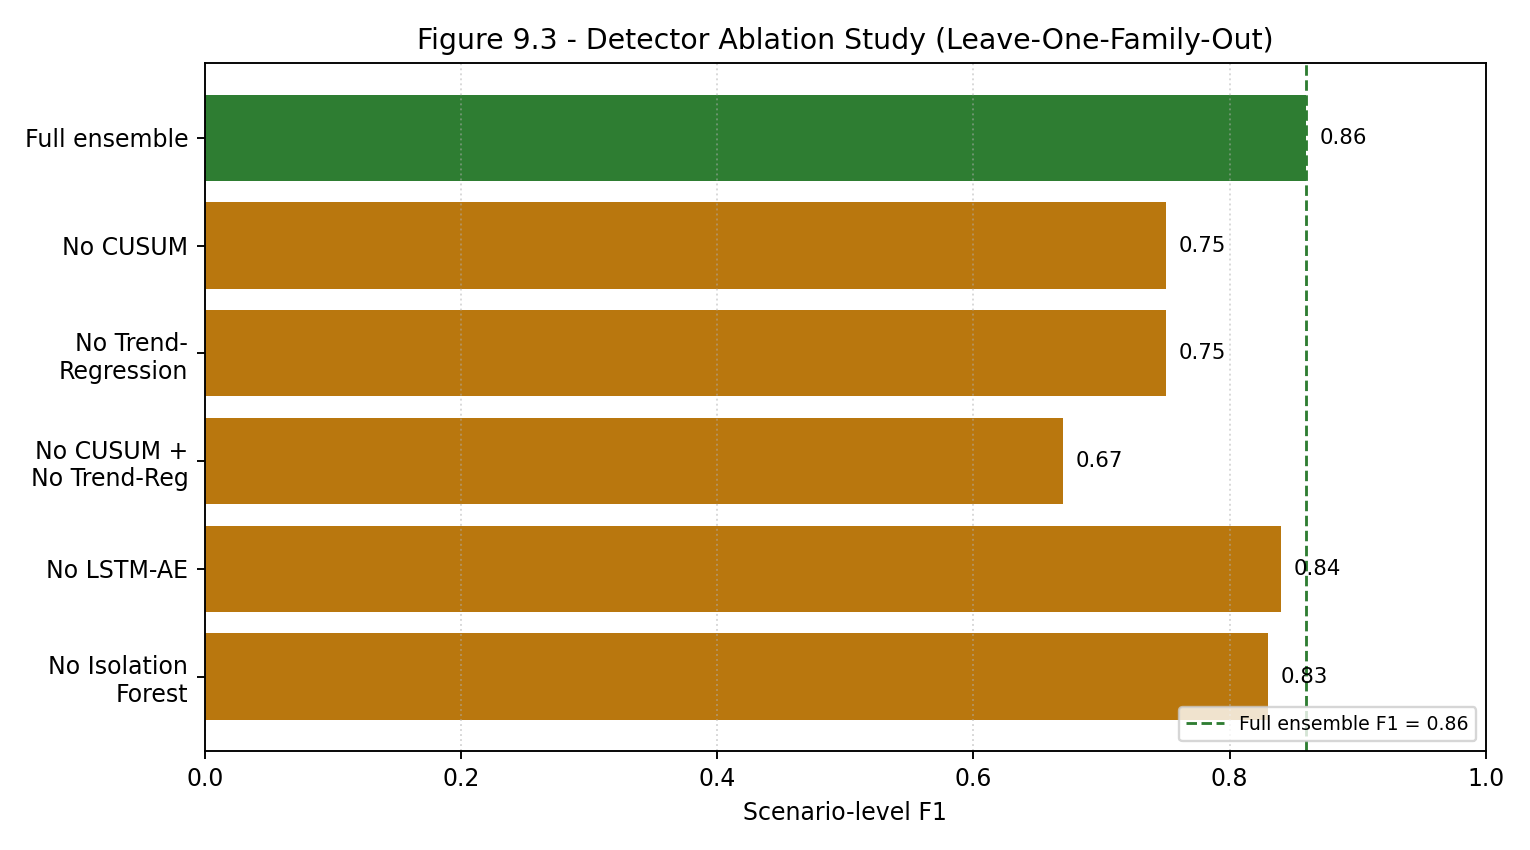
\includegraphics[width=0.85\textwidth]{figures/fig_9_3.png}
    \caption{Detector Ablation Study --- Leave-one-family-out ablation results, showing CUSUM and Trend-Regression as jointly necessary for slow-drift detection.}
    \label{fig:9_3}
\end{figure}

\begin{figure}[htbp]
    \centering
    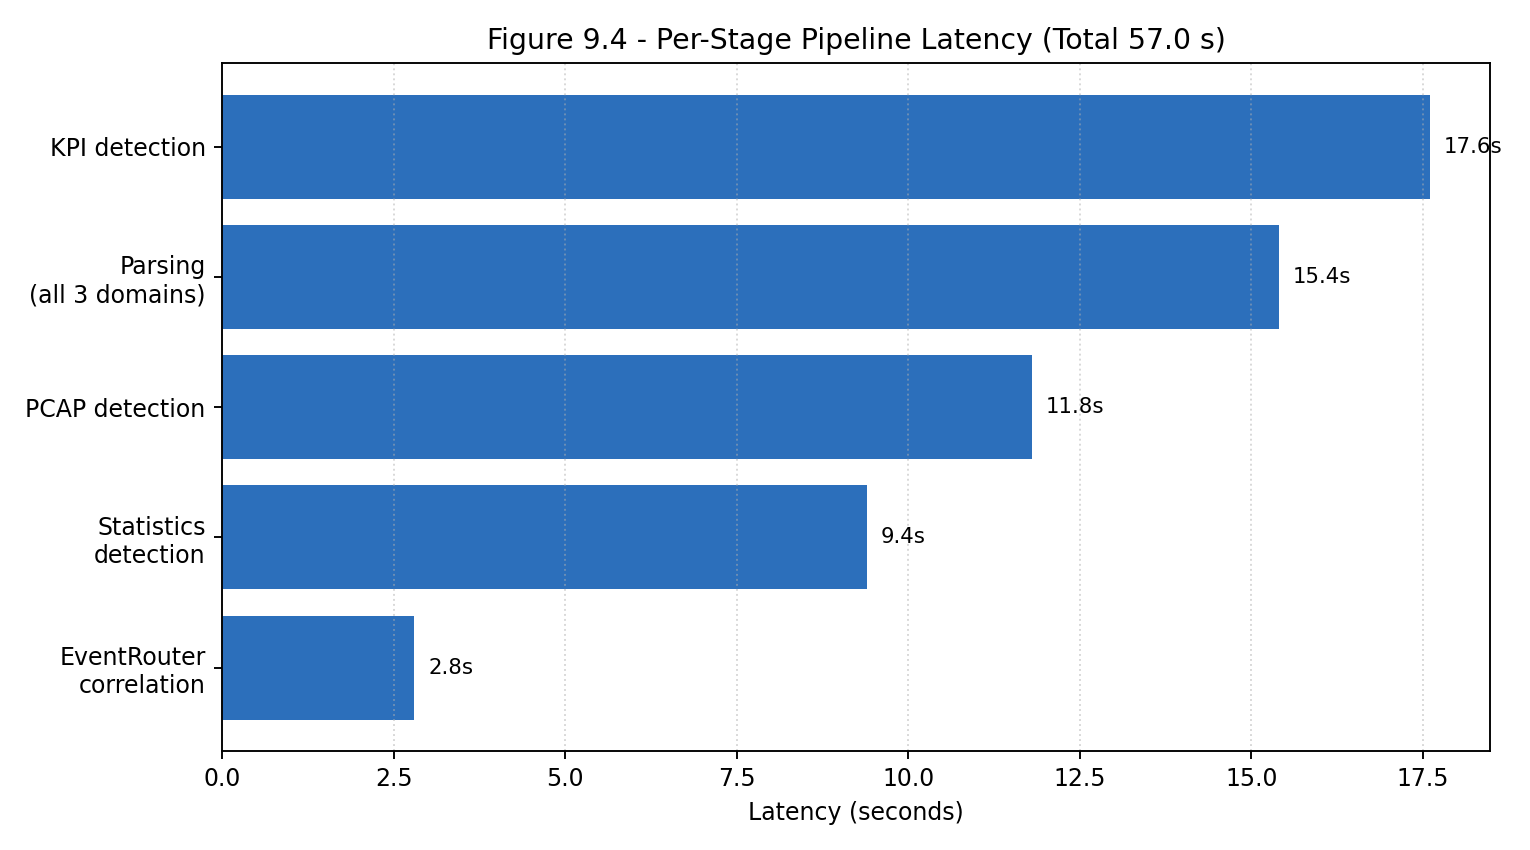
\includegraphics[width=0.85\textwidth]{figures/fig_9_4.png}
    \caption{Pipeline Latency Breakdown by Stage --- Per-stage latency breakdown of the 57-second end-to-end pipeline on the 64-UE dataset.}
    \label{fig:9_4}
\end{figure}

\begin{figure}[htbp]
    \centering
    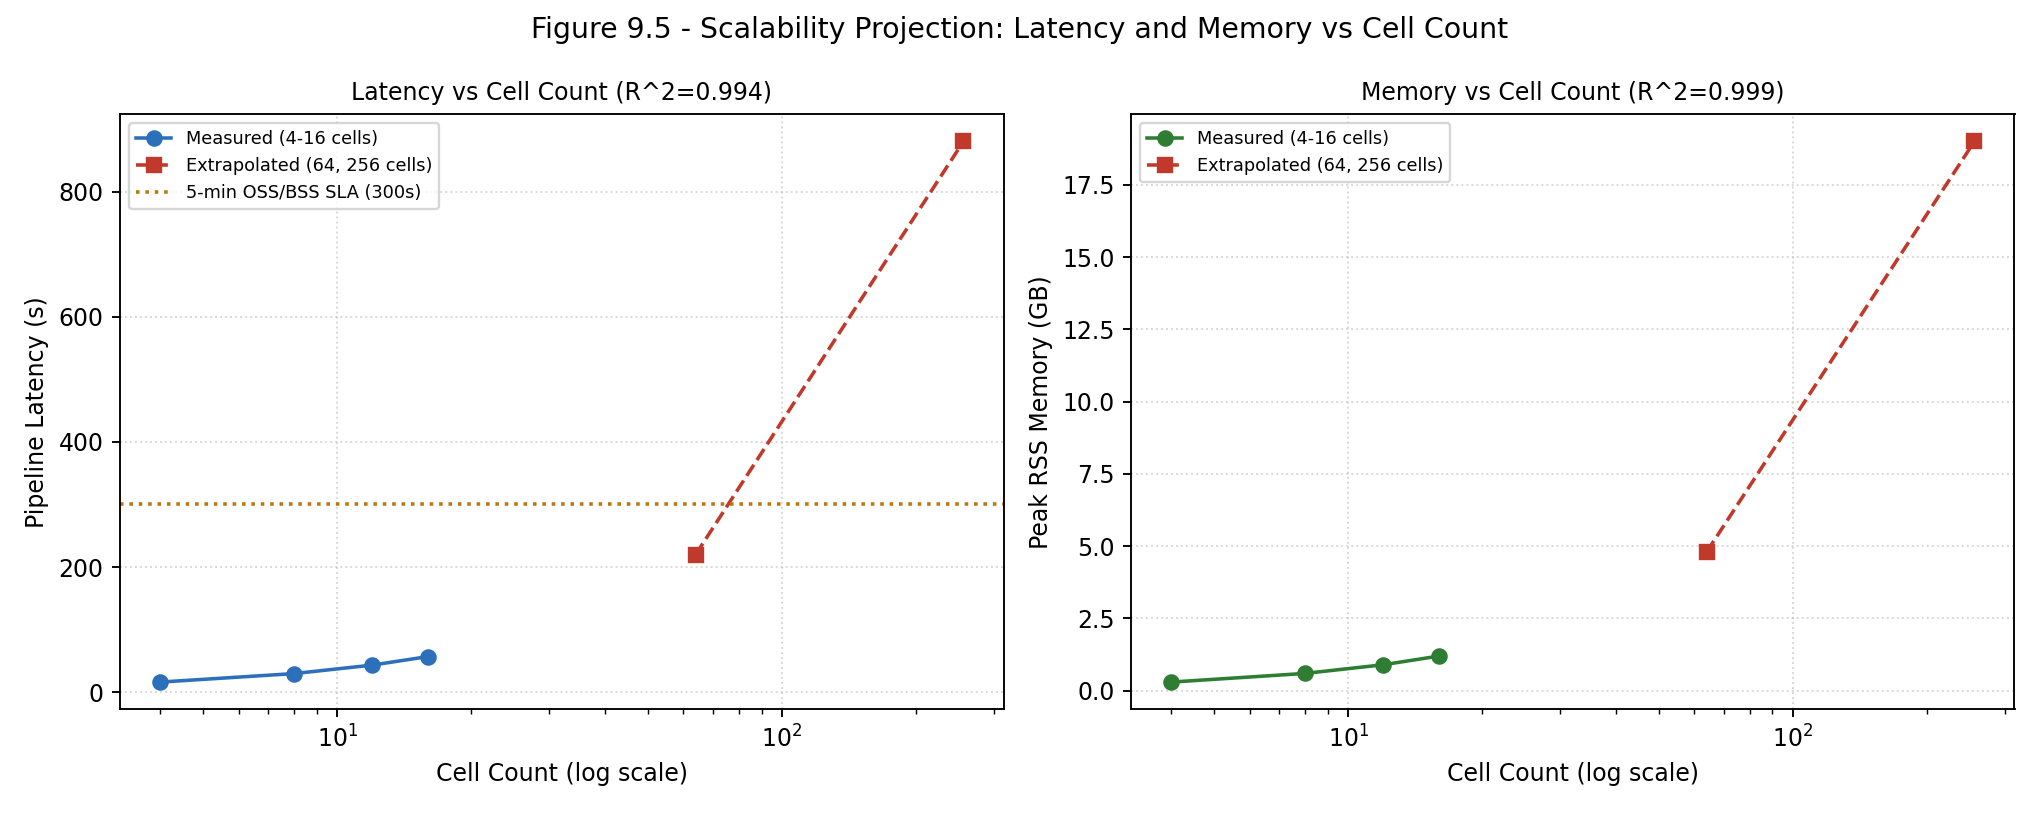
\includegraphics[width=0.85\textwidth]{figures/fig_9_5.png}
    \caption{Scalability Projection (Latency \& Memory vs. Cell Count) --- Measured (4 to 16 cells) and extrapolated (64, 256 cells) pipeline latency and peak memory, with the 5-minute OSS/BSS batch-cycle threshold marked.}
    \label{fig:9_5}
\end{figure}

% ---------------- Chapter 10 ----------------
\begin{figure}[htbp]
    \centering
    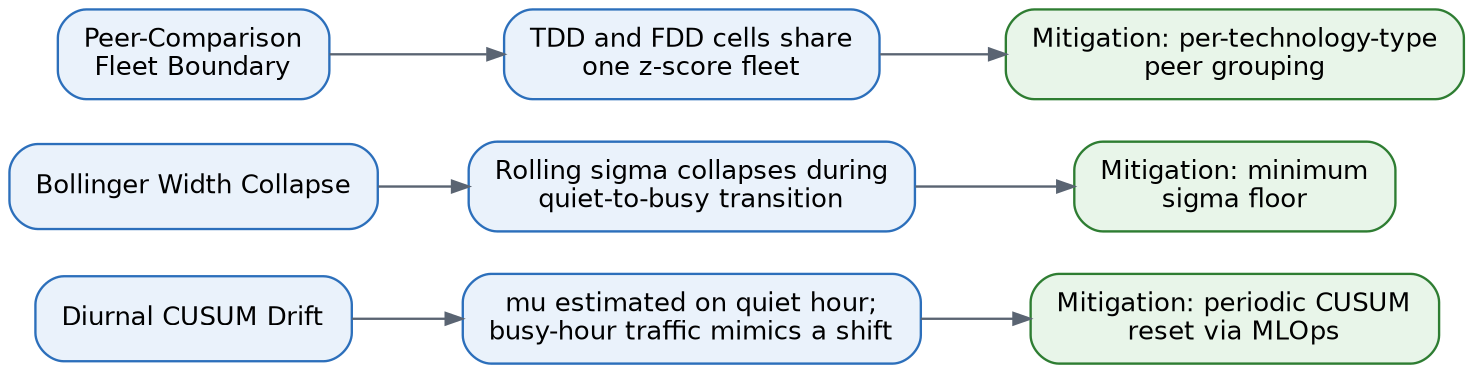
\includegraphics[width=0.85\textwidth]{figures/fig_10_1.png}
    \caption{False-Positive Root-Cause Map --- The three systematic sources of per-record false positives, their underlying mechanism, and the proposed mitigation for each.}
    \label{fig:10_1}
\end{figure}

% ---------------- Chapter 11 ----------------
\begin{figure}[htbp]
    \centering
    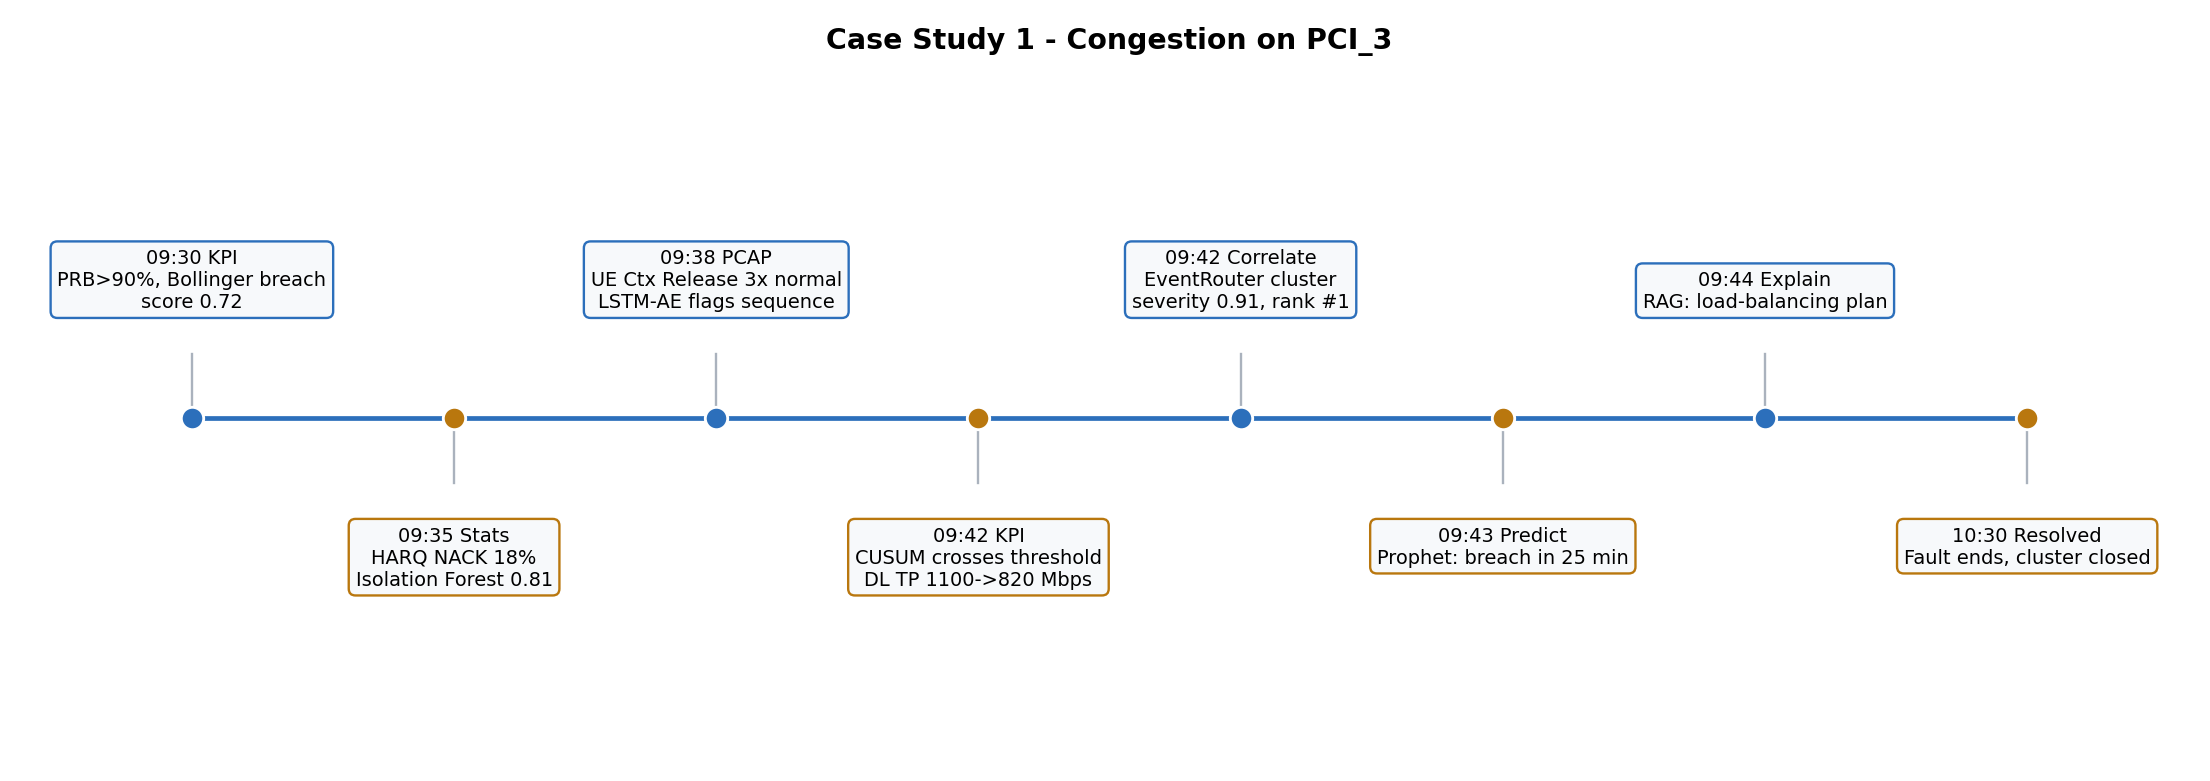
\includegraphics[width=0.85\textwidth]{figures/fig_11_1.png}
    \caption{Case Study 1 Timeline: Congestion on PCI_3 --- End-to-end pipeline trace for the PCI_3 congestion case study, from onset (09:30) to correlated detection (09:42) and explanation (09:44).}
    \label{fig:11_1}
\end{figure}

\begin{figure}[htbp]
    \centering
    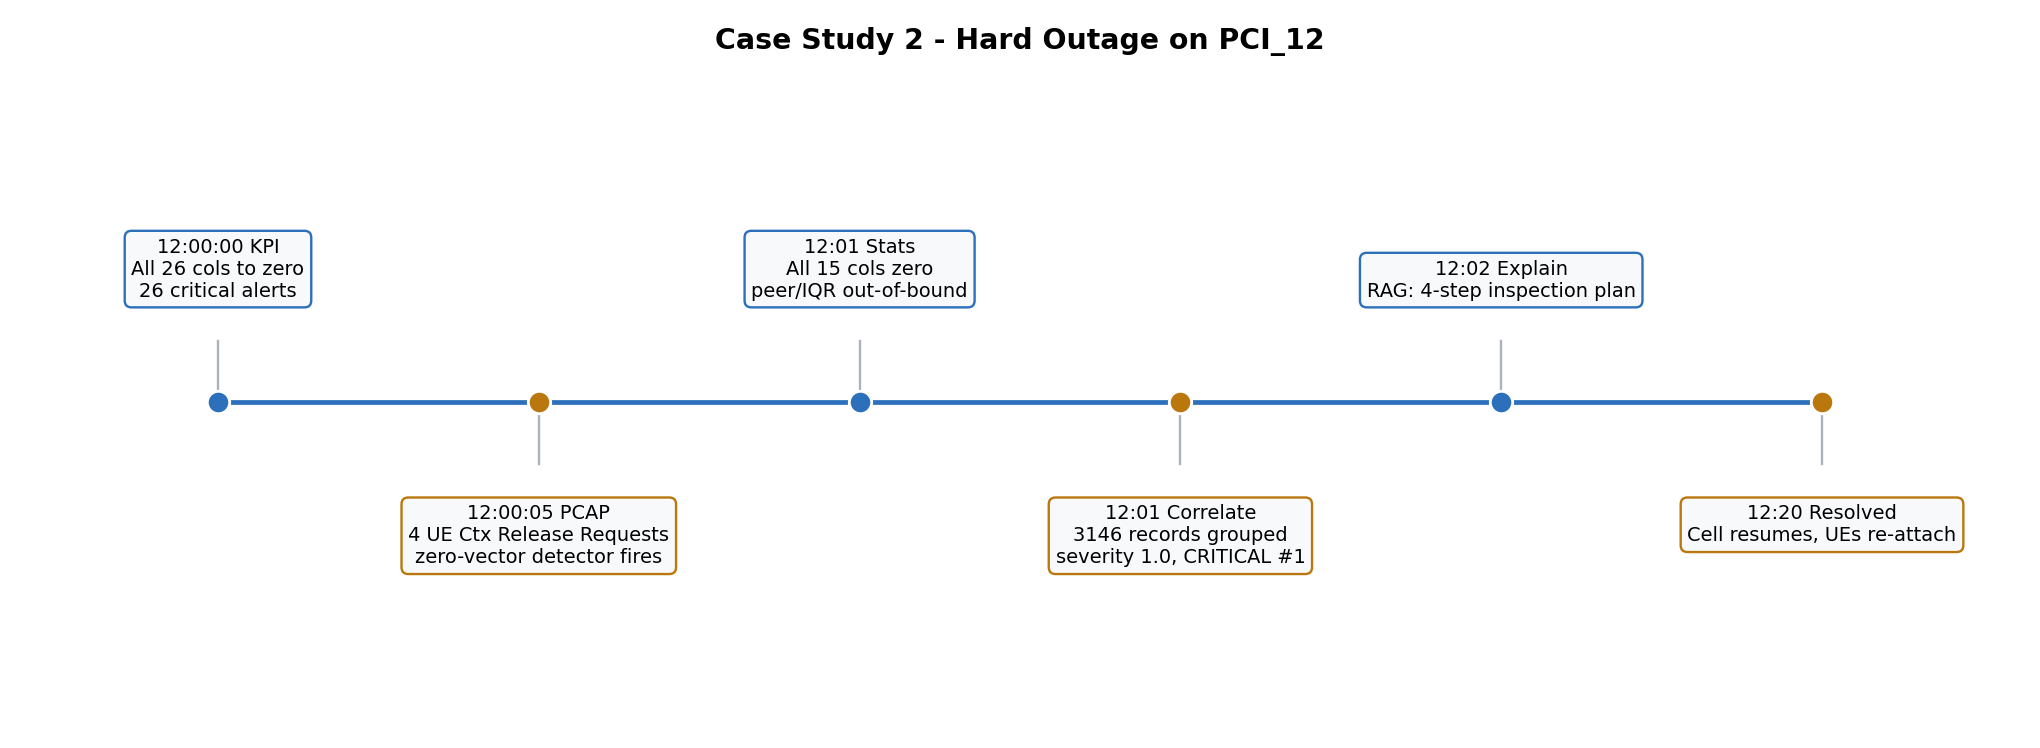
\includegraphics[width=0.85\textwidth]{figures/fig_11_2.png}
    \caption{Case Study 2 Timeline: Hard Outage on PCI_12 --- End-to-end pipeline trace for the PCI_12 hard outage, showing sub-minute detection and immediate severity-1.0 correlation.}
    \label{fig:11_2}
\end{figure}

\begin{figure}[htbp]
    \centering
    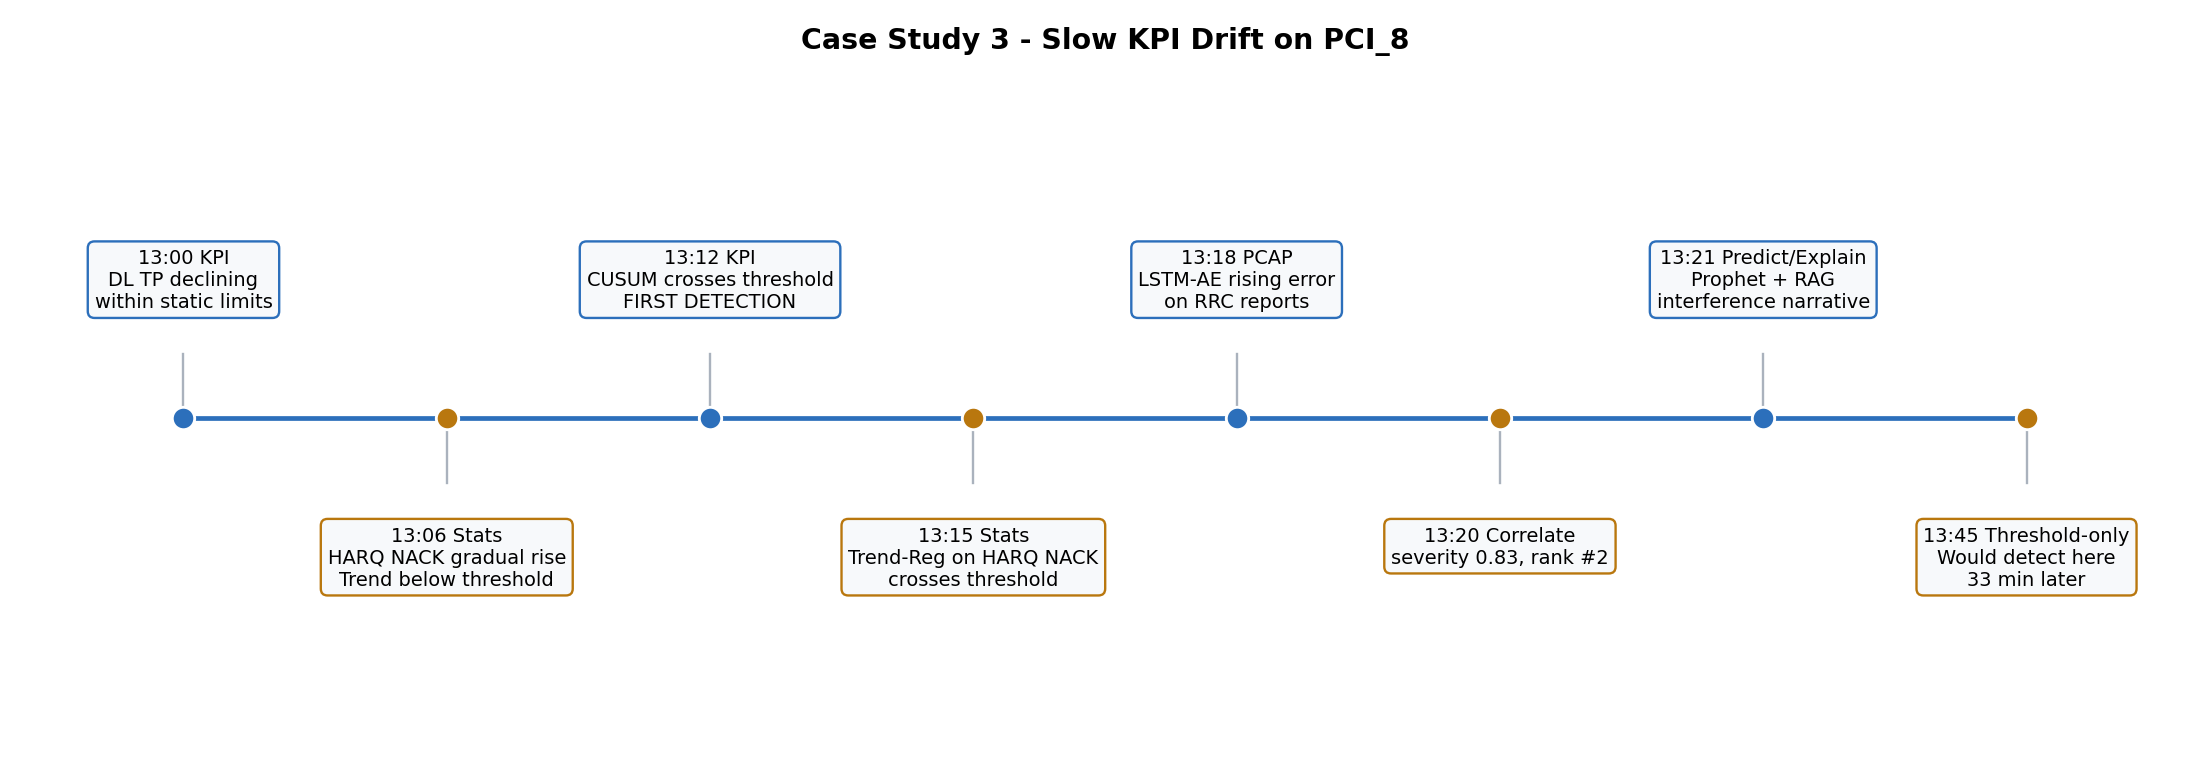
\includegraphics[width=0.85\textwidth]{figures/fig_11_3.png}
    \caption{Case Study 3 Timeline: Slow KPI Drift on PCI_8 --- End-to-end pipeline trace for the PCI_8 slow-drift case study, highlighting the 33-minute early-detection advantage of CUSUM over a threshold-only baseline.}
    \label{fig:11_3}
\end{figure}

% ---------------- Chapter 12 ----------------
\begin{figure}[htbp]
    \centering
    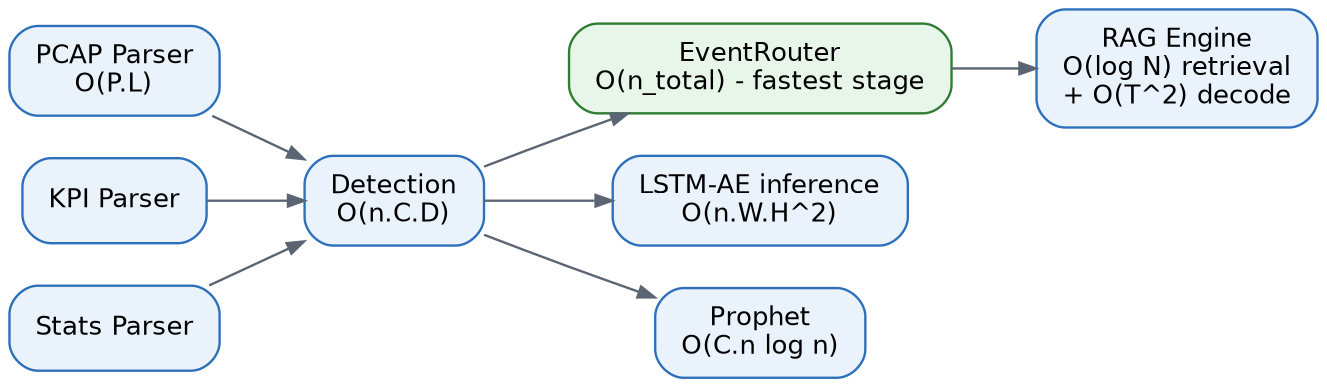
\includegraphics[width=0.85\textwidth]{figures/fig_12_1.png}
    \caption{Module-Level Complexity Overview --- Pipeline stages annotated with their asymptotic time complexity, showing the EventRouter as the fastest stage despite processing the largest input.}
    \label{fig:12_1}
\end{figure}

% ---------------- Chapter 14 ----------------
\begin{figure}[htbp]
    \centering
    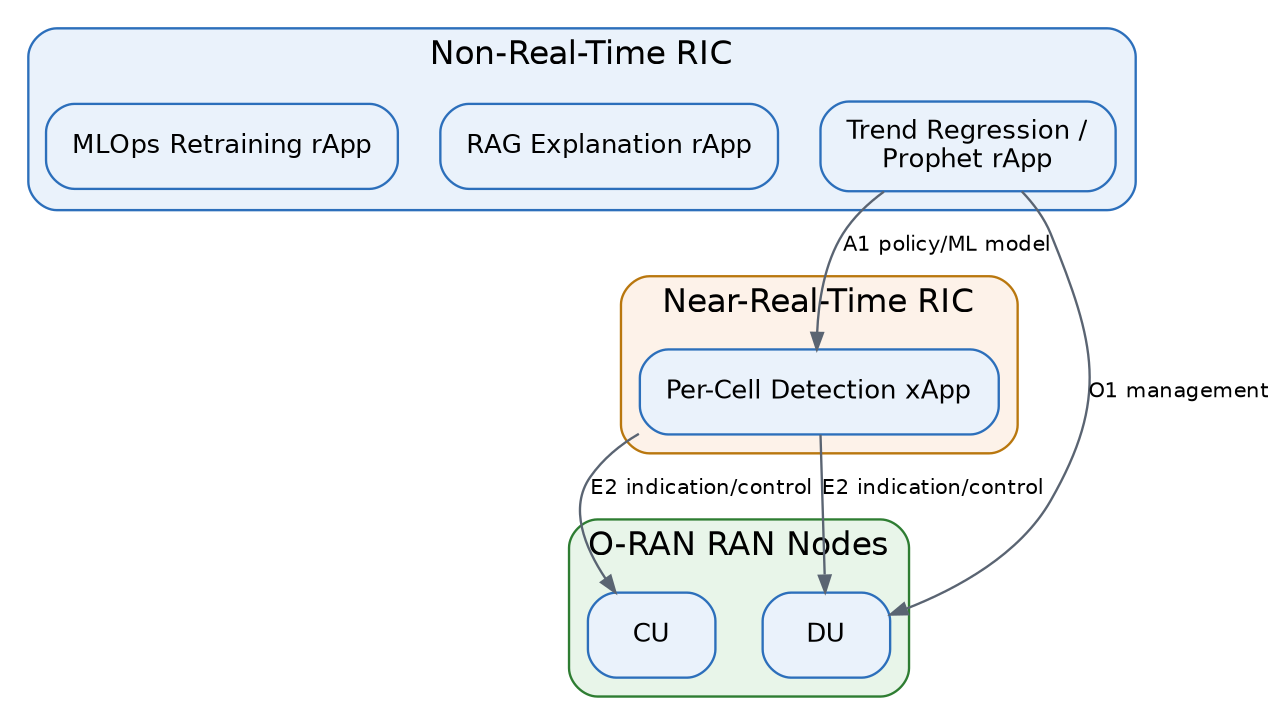
\includegraphics[width=0.85\textwidth]{figures/fig_14_1.png}
    \caption{O-RAN RIC Integration Architecture --- Mapping of the Unified Telecom Analyzer's pipeline modules onto the O-RAN Non-RT RIC (rApps) and Near-RT RIC (xApp) via the A1, O1, and E2 interfaces.}
    \label{fig:14_1}
\end{figure}

\begin{figure}[htbp]
    \centering
    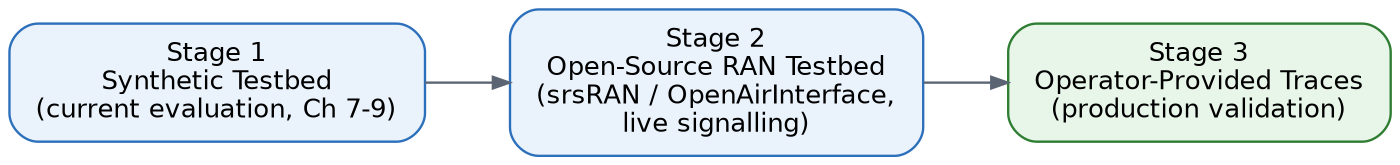
\includegraphics[width=0.85\textwidth]{figures/fig_14_2.png}
    \caption{Staged Production Validation Roadmap --- The staged validation path from the current synthetic evaluation to production deployment on operator traces.}
    \label{fig:14_2}
\end{figure}

\begin{figure}[htbp]
    \centering
    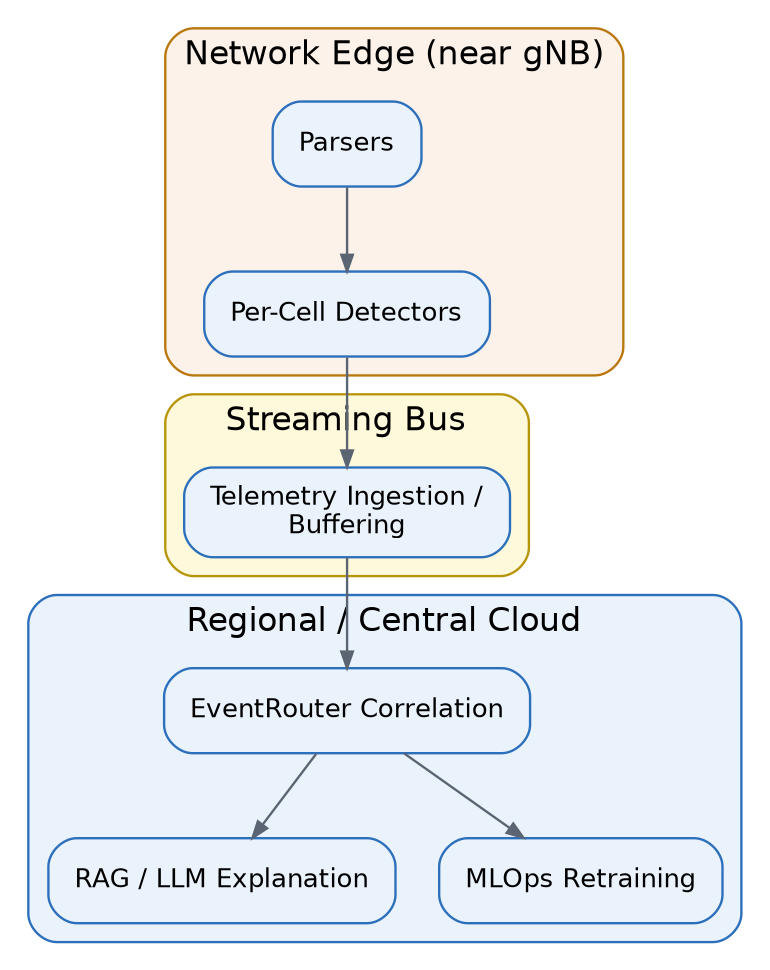
\includegraphics[width=0.85\textwidth]{figures/fig_14_3.png}
    \caption{Cloud-Native Deployment with Edge/Central Split --- Cloud-native deployment topology with latency-sensitive detection at the network edge and heavier RAG/LLM and retraining workloads in central/regional cloud.}
    \label{fig:14_3}
\end{figure}

% ---------------- Chapter 15 ----------------
\begin{figure}[htbp]
    \centering
    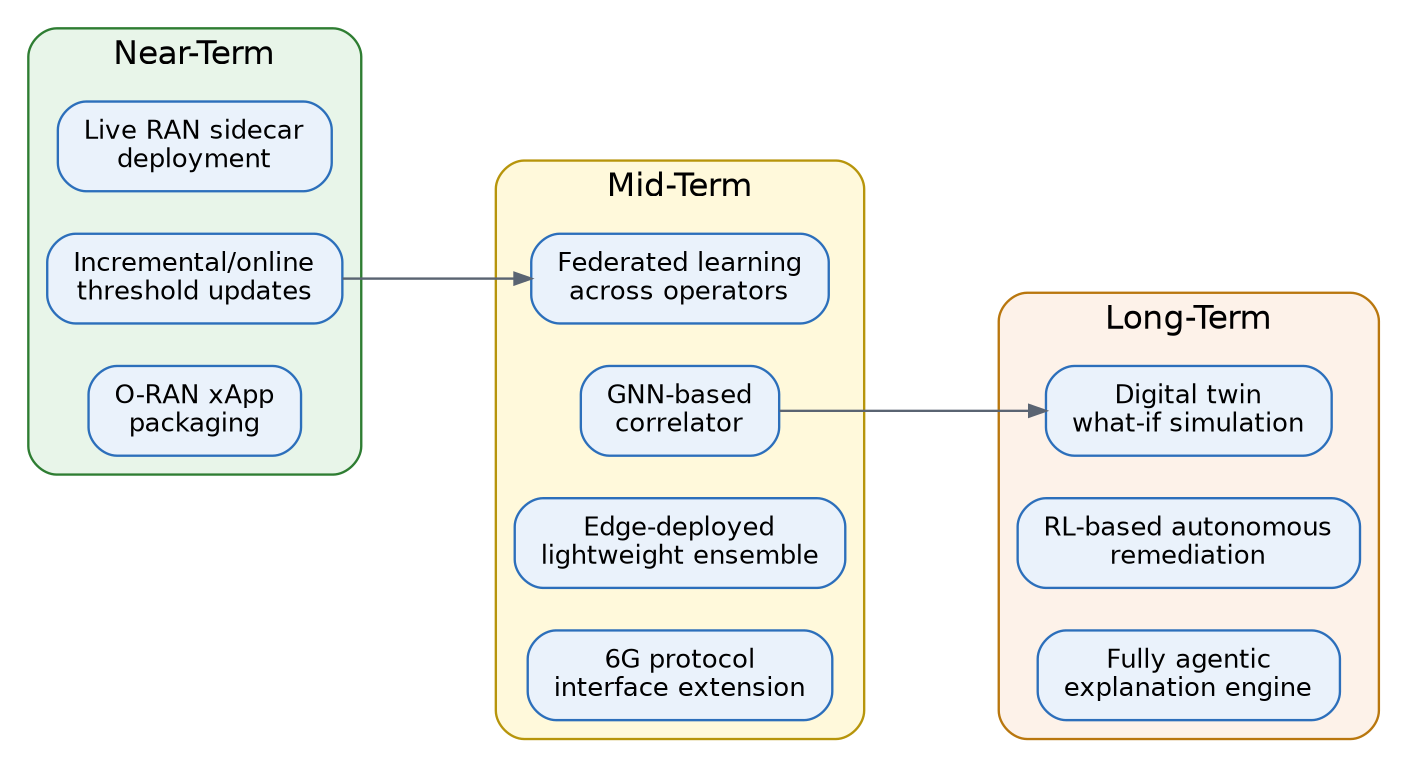
\includegraphics[width=0.85\textwidth]{figures/fig_15_1.png}
    \caption{Future Work Roadmap (Near-Term to Long-Term) --- The ten future work directions grouped by implementation horizon, from near-term engineering extensions to long-term autonomous-network research.}
    \label{fig:15_1}
\end{figure}

% ---------------- Chapter A ----------------
\begin{figure}[htbp]
    \centering
    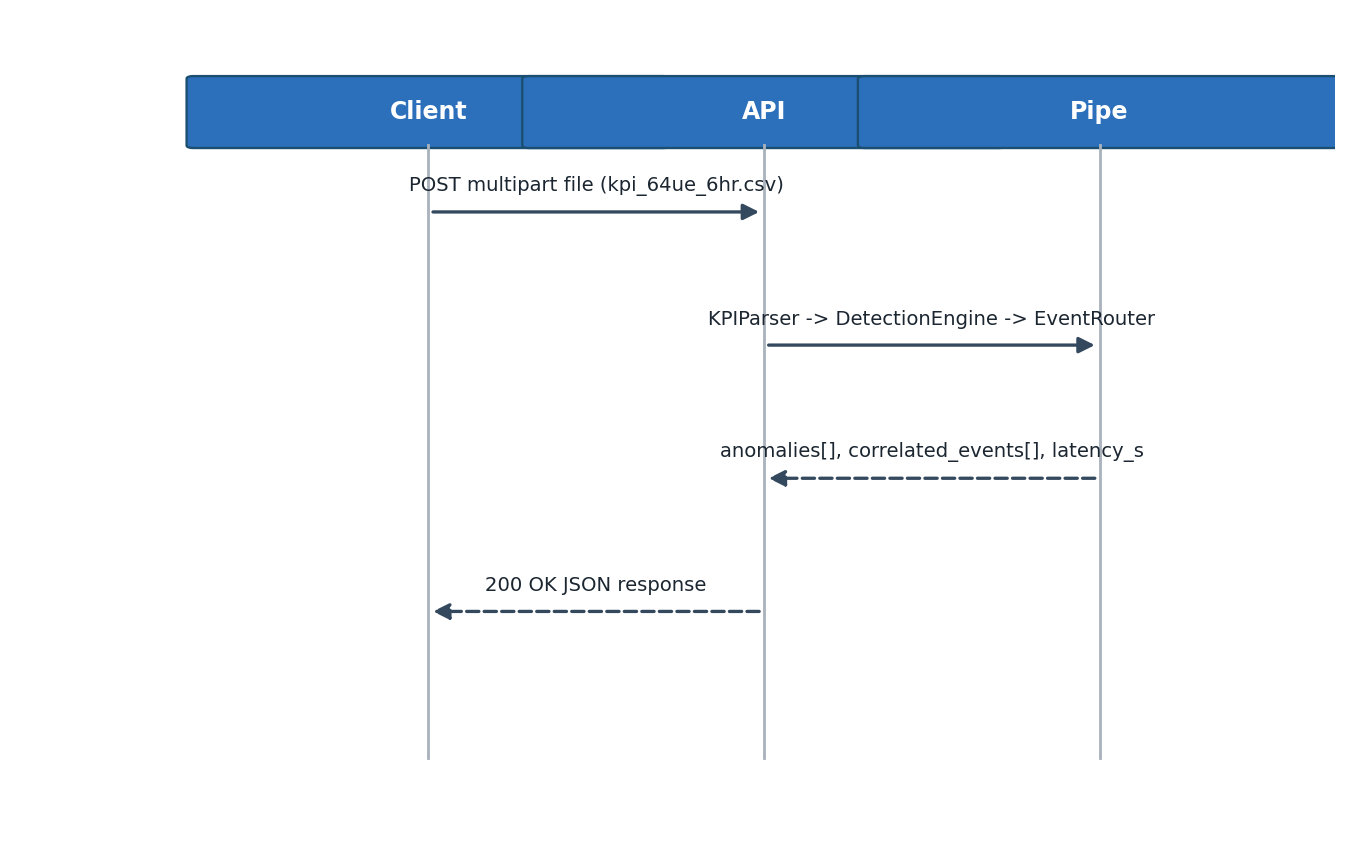
\includegraphics[width=0.85\textwidth]{figures/fig_A_1.png}
    \caption{Sample API Request/Response Flow --- Request/response sequence for the POST /analyze/kpi endpoint, from file upload through pipeline execution to JSON response.}
    \label{fig:A_1}
\end{figure}
